\documentclass[letterpaper,10pt]{book}
% Change to 10 pt
\usepackage{pdfpages}
\usepackage{morewrites}			% to counteract the no write space problem
\setcounter{tocdepth}{6}

\usepackage[framemethod=TikZ]{mdframed}

\usepackage{fancyhdr}

\usepackage{paralist}
\usepackage{amsmath}
\usepackage{amsfonts}
\usepackage{amssymb}
\usepackage{graphicx}

\usepackage{datetime}
%\usepackage{ulem}

%\usepackage[nottoc]{toobibind}

\usepackage[inline]{enumitem}

% Outer margin at 2.50 is exacty correct to fit the ``corruption alert'' tables
\usepackage[inner=1.0in, outer=2.50in, top=2.54cm,bottom=2.54cm, marginparwidth=2.25in]{geometry}

\usepackage{marginnote}
\usepackage{longtable}
\usepackage{booktabs}
\usepackage{xcolor}

\usepackage{soul}

%%%%%%%%%%%%
\definecolor{ForestGreen}{rgb}{0.00,0.29,0.098}
%%%%%%%%%%%%

\usepackage{marginnote}

\usepackage{imakeidx} 
\usepackage[
	backref=true,
	style=numeric,
%	citestyle=numeric,
	backend=bibtex
	]{biblatex}
\usepackage[driverfallback=hypertex,colorlinks=True]{hyperref}
\usepackage{cleveref}

\makeindex[name=scripture,columnsep=20pt, columnseprule=True,columns=3, title=Scripture References]
\makeindex[name=speaker,columnsep=20pt, columnseprule=True,,columns=2, title=Sermon Creator]
\makeindex[name=series,columnsep=20pt, columnseprule=True,,columns=2, title=Sermon Series]
\makeindex[name=date,columnsep=20pt, columnseprule=True,columns=2, title=Sermon Date]
\makeindex[name=event,columnsep=20pt, columnseprule=True,columns=2, title=Event]
\makeindex[name=topic,columnsep=20pt, columnseprule=True,columns=2, title=Topic]
\makeindex[name=AWIP,columnsep=20pt, columnseprule=True,columns=3, title=All Words in Passage]
\makeindex[name=NWIV,columnsep=20pt, columnseprule=True,columns=3, title=Number of Words in Verse]
\makeindex[name=PNIP,columnsep=20pt, columnseprule=True,columns=3, title=Proper Names in Passage]
\makeindex[name=PEIP,columnsep=20pt, columnseprule=True,columns=2, title=Prophetic Events in Passage]
\makeindex[name=TWPAQ,columnsep=20pt, columnseprule=True,columns=1, title=13-Word Phrases and Quotes]
\makeindex[name=PFTTIS,columnsep=20pt, columnseprule=False,columns=3, title=Phrases found 13 times in scripture]
\makeindex[name=WFTTIS,columnsep=20pt, columnseprule=False,columns=3, title=Words found 13 times in scripture]
\makeindex[name=WFITV,columnsep=20pt, columnseprule=False,columns=3, title=Words found in exactly 13 verses]
\makeindex[name=EVENTS,columnsep=20pt, columnseprule=False,columns=2, title=Sermon Log by Place]
\makeindex[name=QUESTIONS,columnsep=20pt, columnseprule=False,columns=2, title=Bible Questions]
\makeindex[name=DOCTRINES,columnsep=20pt, columnseprule=False,columns=2, title=Doctrines]
\makeindex[name=SONGS,columnsep=20pt, columnseprule=False,columns=1, title=Songs]
\makeindex[name=LOCATION,columnsep=20pt, columnseprule=False,columns= 2, title=Location]
\makeindex[name=FACEBOOK,columnsep=20pt, columnseprule=False,columns=2, title=Facebook]
\makeindex[name=DEVOTIONAL,columnsep=20pt, columnseprule=False,columns=2, title=Devotional Items]
%%%%%%%%%%%%%%%%% EXTRA COLORS
\definecolor{champagne}{rgb}{0.97,0.91,0.81}
\definecolor{bone}{rgb}{0.89,0.85,0.79}
\pagestyle{fancy}
\fancyhf{}
\fancyhead[LE,RO]{\today}
\fancyhead[RE,LO]{Daily Bible Reading}
\fancyhead[CE,CO]{-page \thepage  - }

\fancyfoot[CO,CE]{\leftmark}
%\fancyfoot[LE,RO]{CSCE 692, HW1}

\title{DBR\\
Daily \\ Reads}
\author{Keith Anthony \\
\today }
%+/ffffff +   \pagenumbering{gobble}
\bibliography{Bibliographies/All20220122}

\setlength{\fboxsep}{1.0pt}

\usepackage[utf8]{inputenc}
\usepackage{tikz}

\begin{document}
%%%%%%%%%%%% Tile Page

\begin{titlepage}

\begin{flushright}
\rightskip=-2.5cm
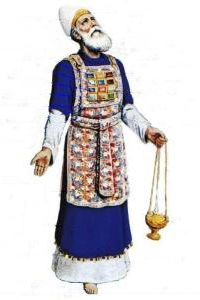
\includegraphics[width=50mm,scale=1.5]{Extras/Melchisedec.jpg}
\vspace{0.4in}  % Create a title for the document and write it in bold font
\LARGE{\textbf{\date}} % Again, do a line break
\linebreak 
% Create a subtitle \large{with Outlines, Statistics, Cross References, and Notes}
\vspace{0.5in}
\begin{flushleft}
\LARGE{Day \#77: Friday, 18  March 2022  \\}\vspace{0.25in}
\LARGE{Judges 13-15 Psalm 77 Proverb 18}
\end{flushleft}
\vspace{0.6in}
\bigskip

\normalsize{Xenia, Oh.\\}
\normalsize{created: \today}
\vspace{1.3in}

\end{flushright}
\end{titlepage}

\newpage 
\tableofcontents\hypertarget{TOC}{}
\listoffigures
\listoftables

\hyphenation{A-bim-e-lech bre-thren E-phra-im  Gib-e-o-nites Jer-u-sa-lem through-out Phil-i-stines The-o-phil-us Am-a-le-kites ven-geance Mesh-el-e-mi-ah onan-ism Phar-a-oh thoughts grev-ous-ness Hach-a-liah adul-ter-er Shad-rach}

%%%%%%%%%%%%%%%%% EXTRA COLORS
%%%%%%%%%%%%%%%%% EXTRA COLORS
%%%%%%%%%%%%%%%%% EXTRA COLORS
\definecolor{champagne}{rgb}{0.97,0.91,0.81}
\definecolor{bone}{rgb}{0.89,0.85,0.79}

\definecolor{ForestGreen}{rgb}{0.00,0.29,0.098}
\definecolor{GIVING}{cmyk}{1,0.0,0.72,.1}

\definecolor{MLPE}{cmyk}{1,1,0,.45}
\definecolor{SOCCER}{cmyk}{.77, 0, .42, .49}
\definecolor{PAYBILL}{cmyk}{0,0.83,0.76,0.07}
\definecolor{SERMON}{cmyk}{.14,.9,0,.30} % aka seance \href{http://www.flatuicolorpicker.com/purple-cmyk-color-model/}{seance}
\definecolor{BIBLE}{cmyk}{0,.17,.74,.17}
\definecolor{WORKBLUE}{cmyk}{1, .5, 0, .6}
\definecolor{myOrange}{cmyk}{0, .4, .98, .03}
\definecolor{myTan}{cmyk}{0.0,.07,.17,.10}
\definecolor{myRed}{cmyk}{0,1,1,0}
\definecolor{myWhite}{cmyk}{0,0,0,0}
\definecolor{BLUESoD}{cmyk}{.97,.84,0,.04}
\definecolor{WHITE}{cmyk}{0,0,0,0}
\definecolor{OLDGOLD}{cmyk}{0.05,0.3,1.00,0}
\definecolor{CASTLETON}{cmyk}{1,0,0.31,0.66}
\definecolor{cadmiumgreen}{rgb}{0.0, 0.42, 0.24}
\definecolor{jungle}{rgb}{0.203,0.4882,0.1718}
\definecolor{MYGOLD}{rgb}{1,.84,0}

\definecolor{MYLIGHTGRAY}{rgb}{.85,.85,.85}

\definecolor{codegreen}{rgb}{0,0.6,0}
\definecolor{codegray}{rgb}{0.5,0.5,0.5}
\definecolor{codepurple}{rgb}{0.58,0,0.82}
\definecolor{backcolour}{rgb}{0.95,0.95,0.92}


\mdfdefinestyle{MyFrame}{%
    linecolor=blue,
    outerlinewidth=2pt,
    roundcorner=5pt,
    innertopmargin=\baselineskip,
    innerbottommargin=\baselineskip,
    innerrightmargin=10pt,
    innerleftmargin=10pt,
    backgroundcolor=gray!25!white}


\mdfdefinestyle{MyFrame2}{%
    linecolor=black,
    outerlinewidth=2pt,
    roundcorner=5pt,
    innertopmargin=\baselineskip,
    innerbottommargin=\baselineskip,
    innerrightmargin=10pt,
    innerleftmargin=10pt,
    backgroundcolor=yellow!25!white}


%%%%%
%% for PFTTIS list
%%%%%

%%% And Joseph said unto
\index[PFTTIS]{And Joseph said unto!Genesis!Gen 40:008}
\index[PFTTIS]{And Joseph said unto!Genesis!Gen 40:012}
\index[PFTTIS]{And Joseph said unto!Genesis!Gen 41:025}
\index[PFTTIS]{And Joseph said unto!Genesis!Gen 42:014}
\index[PFTTIS]{And Joseph said unto!Genesis!Gen 42:018}
\index[PFTTIS]{And Joseph said unto!Genesis!Gen 44:015}
\index[PFTTIS]{And Joseph said unto!Genesis!Gen 45:003}
\index[PFTTIS]{And Joseph said unto!Genesis!Gen 45:004}
\index[PFTTIS]{And Joseph said unto!Genesis!Gen 46:031}
\index[PFTTIS]{And Joseph said unto!Genesis!Gen 48:009}
\index[PFTTIS]{And Joseph said unto!Genesis!Gen 48:018}
\index[PFTTIS]{And Joseph said unto!Genesis!Gen 50:019}
\index[PFTTIS]{And Joseph said unto!Genesis!Gen 50:024}


%%% a shadow
\index[PFTTIS]{a shadow!1Chronicles!1Chr 029:15}
\index[PFTTIS]{a shadow!Job!Job 008:09}
\index[PFTTIS]{a shadow!Job!Job 014:02}
\index[PFTTIS]{a shadow!Job!Job 017:07}
\index[PFTTIS]{a shadow!Psalm!Psa 102:011}
\index[PFTTIS]{a shadow!Psalm!Psa 144:004}
\index[PFTTIS]{a shadow!Ecclesiastes!Eccl 006:012}
\index[PFTTIS]{a shadow!Ecclesiastes!Eccl 008:013}
\index[PFTTIS]{a shadow!Isaiah!Isa 04:006}
\index[PFTTIS]{a shadow!Isaiah!Isa 25:004}
\index[PFTTIS]{a shadow!Jonah!Jnh 04:06}
\index[PFTTIS]{a shadow!Colossians!Col 02:017}
\index[PFTTIS]{a shadow!Hebews!Heb 10:001}

%%% blessed is the man
\index[PFTTIS]{blessed is the man!Psalm!Psa 001:001}
\index[PFTTIS]{blessed is the man!Psalm!Psa 032:002}
\index[PFTTIS]{blessed is the man!Psalm!Psa 034:008}
\index[PFTTIS]{blessed is the man!Psalm!Psa 065:004}
\index[PFTTIS]{blessed is the man!Psalm!Psa 084:005}
\index[PFTTIS]{blessed is the man!Psalm!Psa 084:012}
\index[PFTTIS]{blessed is the man!Psalm!Psa 094:012}
\index[PFTTIS]{blessed is the man!Psalm!Psa 112:001}
\index[PFTTIS]{blessed is the man!Proverbs!Pro 008:034}
\index[PFTTIS]{blessed is the man!Isaiah!Isa 056:002}
\index[PFTTIS]{blessed is the man!Jeremiah!Jer 017:007}
\index[PFTTIS]{blessed is the man!Romans!Rom 004:008}
\index[PFTTIS]{blessed is the man!James!Jam 001:012}


%%% carry them
\index[PFTTIS]{carry them!Leviticus!Lev 14:045}
\index[PFTTIS]{carry them!Numbers!Num 11:012}
\index[PFTTIS]{carry them!Joshua!Jsh 04:003}
\index[PFTTIS]{carry them!1Samuel!1Sam 20:040}
\index[PFTTIS]{carry them!1Kings!1Kng 08:046}
\index[PFTTIS]{carry them!2Chronicles!2Chr 06:036}
\index[PFTTIS]{carry them!Ezra!Ezra 05:015}
\index[PFTTIS]{carry them!Isaiah!Isa 40:011}
\index[PFTTIS]{carry them!Isaiah!Isa 41:016}
\index[PFTTIS]{carry them!Isaiah!Isa 57:013}
\index[PFTTIS]{carry them!Jeremiah!Jer 20:004}
\index[PFTTIS]{carry them!Jeremiah!Jer 20:005}
\index[PFTTIS]{carry them!Jeremiah!Jer 43:012}


\index[PFTTIS]{good tidings!2Samuel!2Sam 18:027}
\index[PFTTIS]{good tidings!1Kings!1Ki 01:042}
\index[PFTTIS]{good tidings!2Kings!2Ki 07:009 (2x)}
\index[PFTTIS]{good tidings!Isaiah!Isa 40:009 (2x)}
\index[PFTTIS]{good tidings!Isaiah!Isa 41:007}
\index[PFTTIS]{good tidings!Isaiah!Isa 52:007}
\index[PFTTIS]{good tidings!Isaiah!Isa 61:001}
\index[PFTTIS]{good tidings!Nahum!Nah 01:005}
\index[PFTTIS]{good tidings!Luke!Lk 02:010}
\index[PFTTIS]{good tidings!1Thessalonians!1Thess 03:006}


%%% dead body
\index[PFTTIS]{dead body!Leviticus!Lev 21:011}
\index[PFTTIS]{dead body!Numbers!Num 06:006}
\index[PFTTIS]{dead body!Numbers!Num 09:006}
\index[PFTTIS]{dead body!Numbers!Num 09:007}
\index[PFTTIS]{dead body!Numbers!Num 09:010}
\index[PFTTIS]{dead body!Numbers!Num 09:011}
\index[PFTTIS]{dead body!Numbers!Num 09:013}
\index[PFTTIS]{dead body!Numbers!Num 09:016}
\index[PFTTIS]{dead body!2Kings!2Ki 08:005}
\index[PFTTIS]{dead body!Isaiah!Isa 26:019}
\index[PFTTIS]{dead body!Jeremiah!Jer 26:023}
\index[PFTTIS]{dead body!Jeremiah!Jer 36:030}
\index[PFTTIS]{dead body!Haggai!Hag 02:013}

%%% great sea
\index[PFTTIS]{great sea!Numbers!Num 34:006}
\index[PFTTIS]{great sea!Numbers!Num 34:007}
\index[PFTTIS]{great sea!Joshua!Jos 01:004}
\index[PFTTIS]{great sea!Joshua!Jos 09:001}
\index[PFTTIS]{great sea!Joshua!Jos 15:012}
\index[PFTTIS]{great sea!Joshua!Jos 15:047}
\index[PFTTIS]{great sea!Joshua!Jos 23:004}
\index[PFTTIS]{great sea!Ezekiel!Eze 47:010}
\index[PFTTIS]{great sea!Ezekiel!Eze 47:015}
\index[PFTTIS]{great sea!Ezekiel!Eze 47:019}
\index[PFTTIS]{great sea!Ezekiel!Eze 47:020}
\index[PFTTIS]{great sea!Ezekiel!Eze 48:028}
\index[PFTTIS]{great sea!Daniel!Dan 07:002}


%%% have forsaken me
\index[PFTTIS]{have forsaken me!Judges!Jdg 10:013}
\index[PFTTIS]{have forsaken me!1Samuel!1Sam 08:008}
\index[PFTTIS]{have forsaken me!1Kings!1Ki 11:033}
\index[PFTTIS]{have forsaken me!2Kings!2Ki 22:017}
\index[PFTTIS]{have forsaken me!2Chronicles!2Chr 12:005}
\index[PFTTIS]{have forsaken me!2Chronicles!2Chr 34:025}
\index[PFTTIS]{have forsaken me!Jeremiah!Jer 01:016}
\index[PFTTIS]{have forsaken me!Jeremiah!Jer 02:013}
\index[PFTTIS]{have forsaken me!Jeremiah!Jer 05:007}
\index[PFTTIS]{have forsaken me!Jeremiah!Jer 05:019}
\index[PFTTIS]{have forsaken me!Jeremiah!Jer 16:011 (2x)}
\index[PFTTIS]{have forsaken me!Jeremiah!Jer 19:004}

%%% no king
\index[PFTTIS]{no king!Judges!Jdg 17:06}
\index[PFTTIS]{no king!Judges!Jdg 18:01}
\index[PFTTIS]{no king!Judges!Jdg 19:01}
\index[PFTTIS]{no king!Judges!Jdg 21:25}
\index[PFTTIS]{no king!1Kings!1Ki 22:47}
\index[PFTTIS]{no king!2Kings!2Ki 23:25}
\index[PFTTIS]{no king!Nehemiah!Neh 13:26}
\index[PFTTIS]{no king!Psalms!Psa 033:016}
\index[PFTTIS]{no king!Proverbs!Pro 30:27}
\index[PFTTIS]{no king!Daniel!Dan 02:10}
\index[PFTTIS]{no king!Hosea!Hos 10:03}
\index[PFTTIS]{no king!Micah!Mic 04:09}
\index[PFTTIS]{no king!John!Jhn 19:15}


%%% rebellious house
\index[PFTTIS]{rebellious house!Exodus!Exo 02:005}
\index[PFTTIS]{rebellious house!Exodus!Exo 02:006}
\index[PFTTIS]{rebellious house!Exodus!Exo 02:008}
\index[PFTTIS]{rebellious house!Exodus!Exo 03:009}
\index[PFTTIS]{rebellious house!Exodus!Exo 03:026}
\index[PFTTIS]{rebellious house!Exodus!Exo 03:027}
\index[PFTTIS]{rebellious house!Exodus!Exo 12:002 (2x)}
\index[PFTTIS]{rebellious house!Exodus!Exo 12:003}
\index[PFTTIS]{rebellious house!Exodus!Exo 12:009}
\index[PFTTIS]{rebellious house!Exodus!Exo 12:025}
\index[PFTTIS]{rebellious house!Exodus!Exo 17:012}
\index[PFTTIS]{rebellious house!Exodus!Exo 24:003}

%%% seek him
\index[PFTTIS]{seek him!Deuteronomy!Deu 04:029}\index[PFTTIS]{seek him!1Samuel!1Sam 23:025}
\index[PFTTIS]{seek him!1Chronicles!1Chr 28:009}
\index[PFTTIS]{seek him!2Chronicles!1Chr 15:002}
\index[PFTTIS]{seek him!Ezra!Ezr 08:022}
\index[PFTTIS]{seek him!Psalms!Psa 022:026}
\index[PFTTIS]{seek him!Psalms!Psa 024:006}
\index[PFTTIS]{seek him!Psalms!Psa 119:002}
\index[PFTTIS]{seek him!SoS!SoS 03:002}
\index[PFTTIS]{seek him!SoS!SoS 06:001}
\index[PFTTIS]{seek him!Hosea!Hos 07:010}
\index[PFTTIS]{seek him!Amos!Amo 05:008}
\index[PFTTIS]{seek him!Hebrews!Heb 11:0063}


%%% seek ye
\index[PFTTIS]{seek ye!Isaiah!Isa 34:016}
\index[PFTTIS]{seek ye!Isaiah!Isa 45:019}
\index[PFTTIS]{seek ye!Isaiah!Isa 55:006}
\index[PFTTIS]{seek ye!Amos!Amos 5:004}
\index[PFTTIS]{seek ye!John!John 1:38}
\index[PFTTIS]{seek ye!John!John 18:4}
\index[PFTTIS]{seek ye!John!John 18:7}
\index[PFTTIS]{seek ye!Matthew!Matt 6:33}
\index[PFTTIS]{seek ye!Numbers!Num 16:10}
\index[PFTTIS]{seek ye!Luke!Luke 12:31}
\index[PFTTIS]{seek ye!Luke!Luke 24:5}
\index[PFTTIS]{seek ye!Psalm!Psa 27:8}
\index[PFTTIS]{seek ye!Zephaniah!Zeph 2:3}

%%% the uncircumcised
\index[PFTTIS]{the uncircumcised!Genesis!Gen 17:014}
\index[PFTTIS]{the uncircumcised!Judges!Jdg 14:003}
\index[PFTTIS]{the uncircumcised!Judges!Jdg 15:018}
\index[PFTTIS]{the uncircumcised!2Samuel!2Sam 01:020}
\index[PFTTIS]{the uncircumcised!Isaiah!Isa 02:001}
\index[PFTTIS]{the uncircumcised!Jeremiah!Jer 09:025}
\index[PFTTIS]{the uncircumcised!Ezekiel!Eze 28:010}
\index[PFTTIS]{the uncircumcised!Ezekiel!Eze 31:018}
\index[PFTTIS]{the uncircumcised!Ezekiel!Eze 32:019}
\index[PFTTIS]{the uncircumcised!Ezekiel!Eze 32:027}
\index[PFTTIS]{the uncircumcised!Ezekiel!Eze 32:028}
\index[PFTTIS]{the uncircumcised!Ezekiel!Eze 32:029}
\index[PFTTIS]{the uncircumcised!Ezekiel!Eze 32:032}

%%% worship him
\index[PFTTIS]{worship him!Psalms!Psa 97:007}
\index[PFTTIS]{worship him!Zephaniah!Zeph 02:011}
\index[PFTTIS]{worship him!Matthew!Matt 02:002}
\index[PFTTIS]{worship him!Matthew!Matt 02:008}
\index[PFTTIS]{worship him!John!John 04:023}
\index[PFTTIS]{worship him!John!John 04:024 (2x)} 
\index[PFTTIS]{worship him!Acts!Acts 17:023}
\index[PFTTIS]{worship him!Hebrews!Heb 01:006}
\index[PFTTIS]{worship him!Revelation!Rev 04:010}
\index[PFTTIS]{worship him!Revelation!Rev 13:008}
\index[PFTTIS]{worship him!Revelation!Rev 14:007}
\index[PFTTIS]{worship him!Revelation!Rev 19:010}


%%%%%
%% for PFTTIS list
%%%%%

%%% afflictions
\index[WFTTIS]{afflictions!Psalms!Psa 34:019}
\index[WFTTIS]{afflictions!Psalms!Psa 132:001}
\index[WFTTIS]{afflictions!Acts!Acts 07:010}
\index[WFTTIS]{afflictions!Acts!Acts 20:023}
\index[WFTTIS]{afflictions!2Corinthians!2Cor 06:004}
\index[WFTTIS]{afflictions!Colossians!Col 01:024}
\index[WFTTIS]{afflictions!1Thessalonians!1Thess 03:003}
\index[WFTTIS]{afflictions!2Timothy!2Tim 01:008}
\index[WFTTIS]{afflictions!2Timothy!2Tim 03:011}
\index[WFTTIS]{afflictions!2Timothy!2Tim 04:005}
\index[WFTTIS]{afflictions!Hebrews!Heb 10:032}
\index[WFTTIS]{afflictions!Hebrews!Heb 10:033}
\index[WFTTIS]{afflictions!1Peter!1Pet 05:009}

%%% acsend
\index[WFTTIS]{acsend!Joshua!Jos 06:05}
\index[WFTTIS]{acsend!Psalm!Psa 024:003}
\index[WFTTIS]{acsend!Psalm!Psa 135:007}
\index[WFTTIS]{acsend!Psalm!Psa 139:008}
\index[WFTTIS]{acsend!Isaiah!Isa 14:013}
\index[WFTTIS]{acsend!Isaiah!Isa 14:014}
\index[WFTTIS]{acsend!Jeremiah!Jer 10:013}
\index[WFTTIS]{acsend!Jeremiah!Jer 51:016}
\index[WFTTIS]{acsend!Ezekiel!Eze 38:009}
\index[WFTTIS]{acsend!John!John 06:062}
\index[WFTTIS]{acsend!John!John 20:017}
\index[WFTTIS]{acsend!Romans!Rom 10:006}
\index[WFTTIS]{acsend!Revelation!Rev 17:008}

%%% Assyrian
\index[WFTTIS]{Assyrian!Isaiah!Isa 10:005}
\index[WFTTIS]{Assyrian!Isaiah!Isa 10:024}
\index[WFTTIS]{Assyrian!Isaiah!Isa 14:025}
\index[WFTTIS]{Assyrian!Isaiah!Isa 19:023}
\index[WFTTIS]{Assyrian!Isaiah!Isa 23:013}
\index[WFTTIS]{Assyrian!Isaiah!Isa 30:031}
\index[WFTTIS]{Assyrian!Isaiah!Isa 31:008}
\index[WFTTIS]{Assyrian!Isaiah!Isa 52:004}
\index[WFTTIS]{Assyrian!Ezekiel!Eze 31:003}
\index[WFTTIS]{Assyrian!Hosea!Hos 05:013}
\index[WFTTIS]{Assyrian!Hosea!Hos 11:005}
\index[WFTTIS]{Assyrian!Micah!Hos 05:005}
\index[WFTTIS]{Assyrian!Micah!Hos 05:006}

%%% blot
\index[WFTTIS]{blot!Exodus!Exo 32:032}
\index[WFTTIS]{blot!Exodus!Exo 32:033}
\index[WFTTIS]{blot!Numbers!Num 05:026}
\index[WFTTIS]{blot!Deuteronomy!Deut 09:014}
\index[WFTTIS]{blot!Deuteronomy!Deut 25:019}
\index[WFTTIS]{blot!Deuteronomy!Deut 29:020}
\index[WFTTIS]{blot!2Kings!2Ki 14:027}
\index[WFTTIS]{blot!Job!Job 31:007}
\index[WFTTIS]{blot!Psalms!Psa 51:001}
\index[WFTTIS]{blot!Psalms!Psa 51:009}
\index[WFTTIS]{blot!Proverbs!Pro 09:007}
\index[WFTTIS]{blot!Jeremiah!Jer 18:023}
\index[WFTTIS]{blot!Revelation!Rev 03:005}


%%% chain
\index[WFTTIS]{chain!Genesis!Gen 41:042}
\index[WFTTIS]{chain!1Kings!1Ki 07:017}
\index[WFTTIS]{chain!Psalms!Psa 73:006}
\index[WFTTIS]{chain!SoS!Sos 04:009}
\index[WFTTIS]{chain!Lamentations!Lam 03:007}
\index[WFTTIS]{chain!Ezekiel!Eze 07:023}
\index[WFTTIS]{chain!Ezekiel!Eze 16:011}
\index[WFTTIS]{chain!Daniel!Dan 05:007}
\index[WFTTIS]{chain!Daniel!Dan 05:016}
\index[WFTTIS]{chain!Daniel!Dan 05:029}
\index[WFTTIS]{chain!Acts!Acts 28:020}
\index[WFTTIS]{chain!2Timothy!2Tim 01:016}
\index[WFTTIS]{chain!Revelation!Rev 20:001}


%%% controversy
\index[WFTTIS]{controversy!Deuteronomy!Deu 17:008}
\index[WFTTIS]{controversy!Deuteronomy!Deu 19:017}
\index[WFTTIS]{controversy!Deuteronomy!Deu 21:005}
\index[WFTTIS]{controversy!Deuteronomy!Deu 25:001}
\index[WFTTIS]{controversy!2Samuel!2Sam 15:002}
\index[WFTTIS]{controversy!Isaiah!Isa 34:008}
\index[WFTTIS]{controversy!Jeremiah!Jer 25:031}
\index[WFTTIS]{controversy!Ezekiel!Eze 44:024}
\index[WFTTIS]{controversy!Hosea!Hos 04:001}
\index[WFTTIS]{controversy!Hosea!Hos 12:002}
\index[WFTTIS]{controversy!Micah!Mic 06:002 (2x)}
\index[WFTTIS]{controversy!1Timothy!1Tim 03:016}


%%% Dagon/Dagon's
\index[WFTTIS]{Dagon!Judges!Jdg 16:023}
\index[WFTTIS]{Dagon!1Samuel!1Sam 05:002 (2x)}
\index[WFTTIS]{Dagon!1Samuel!1Sam 05:003 (2x)}
\index[WFTTIS]{Dagon!1Samuel!1Sam 05:004 (3x)}
\index[WFTTIS]{Dagon!1Samuel!1Sam 05:005 (3x)}
\index[WFTTIS]{Dagon!1Samuel!1Sam 05:007}
\index[WFTTIS]{Dagon!1Chronicles!1Chr 10:010}

%%% disobedient
\index[WFTTIS]{disobedient!1Kings!1Ki 13:026}
\index[WFTTIS]{disobedient!Nehemiah!Neh 09:026}
\index[WFTTIS]{disobedient!Luke!Luke 01:017}
\index[WFTTIS]{disobedient!Acts!Acts 26:019}
\index[WFTTIS]{disobedient!Romans!Rom 01:030}
\index[WFTTIS]{disobedient!Romans!Rom 10:021}
\index[WFTTIS]{disobedient!1Timothy!1Tim 01:009}
\index[WFTTIS]{disobedient!2Timothy!2Tim 03:002}
\index[WFTTIS]{disobedient!Titus!Titus 01:016}
\index[WFTTIS]{disobedient!Titus!Titus 03:003}
\index[WFTTIS]{disobedient!1Peter!1Pet 02:007}
\index[WFTTIS]{disobedient!1Peter!1Pet 02:008}
\index[WFTTIS]{disobedient!1Peter!1Pet 03:020}


%%% doubt
\index[WFTTIS]{doubt!Genesis!Gen 37:033}
\index[WFTTIS]{doubt!Deuteronomy!Deu 28:066}
\index[WFTTIS]{doubt!Job!Job 12:002}
\index[WFTTIS]{doubt!Matthew!Matt 14:031}
\index[WFTTIS]{doubt!Matthew!Matt 21:021}
\index[WFTTIS]{doubt!Mark!Mk 11:023}
\index[WFTTIS]{doubt!Luke!Lk 11:020}
\index[WFTTIS]{doubt!John!Jhn 10:024}
\index[WFTTIS]{doubt!Acts!Acts 02:012}
\index[WFTTIS]{doubt!Acts!Acts 28:004}
\index[WFTTIS]{doubt!1Corinthians!1Cor 09:010}
\index[WFTTIS]{doubt!Galatians!Gal 04:020}
\index[WFTTIS]{doubt!1John!1Jhn 02:019}


%%% dungeon
\index[WFTTIS]{dungeon!Genesis!Gen 40:015}
\index[WFTTIS]{dungeon!Genesis!Gen 41:014}
\index[WFTTIS]{dungeon!Exodus!Exo 12:029}
\index[WFTTIS]{dungeon!Jeremiah!Jer 37:016}
\index[WFTTIS]{dungeon!Jeremiah!Jer 38:006 (2x)}
\index[WFTTIS]{dungeon!Jeremiah!Jer 38:007}
\index[WFTTIS]{dungeon!Jeremiah!Jer 38:009}
\index[WFTTIS]{dungeon!Jeremiah!Jer 38:010}
\index[WFTTIS]{dungeon!Jeremiah!Jer 38:011}
\index[WFTTIS]{dungeon!Jeremiah!Jer 38:013}
\index[WFTTIS]{dungeon!Lamentations!Lam 03:053}
\index[WFTTIS]{dungeon!Lamentations!Lam 03:055}


%%% error
\index[WFTTIS]{error!2Samuel!2Sam 06:007}
\index[WFTTIS]{error!Job!Job 19:004}
\index[WFTTIS]{error!Ecclesiastes!Ecc 05:006}
\index[WFTTIS]{error!Ecclesiastes!Ecc 10:005}
\index[WFTTIS]{error!Isaiah!Isa 32:006}
\index[WFTTIS]{error!Daniel!Dan 06:004}
\index[WFTTIS]{error!Matthew!Matt 27:064}
\index[WFTTIS]{error!Romans!Rom 01:027}
\index[WFTTIS]{error!James!Jam 05:020}
\index[WFTTIS]{error!2Peter!2Pet 02:018}
\index[WFTTIS]{error!2Peter!2Pet 03:017}
\index[WFTTIS]{error!1John!1Jn 04:006}
\index[WFTTIS]{error!Jude!Jude 01:011}

%%% fourish
\index[WFTTIS]{fourish!Psalms!Psa 072:007}
\index[WFTTIS]{fourish!Psalms!Psa 072:016}
\index[WFTTIS]{fourish!Psalms!Psa 092:007}
\index[WFTTIS]{fourish!Psalms!Psa 092:012}
\index[WFTTIS]{fourish!Psalms!Psa 092:013}
\index[WFTTIS]{fourish!Psalms!Psa 132:018}
\index[WFTTIS]{fourish!Proverbs!Pro 11:28}
\index[WFTTIS]{fourish!Proverbs!Pro 14:11}
\index[WFTTIS]{fourish!Ecclesiastes!Ecc 12:05}
\index[WFTTIS]{fourish!SongOfSolomon!SOS 07:12}
\index[WFTTIS]{fourish!Isaiah!Isa 17:11}
\index[WFTTIS]{fourish!Isaiah!Isa 66:14}
\index[WFTTIS]{fourish!Ezekiel!Eze 17:24}




%%% giants
\index[WFTTIS]{giants!Genesis!Gen 06:004}
\index[WFTTIS]{giants!Numbers!Num 13:033}
\index[WFTTIS]{giants!Deuteronomy!Deut 02:011}
\index[WFTTIS]{giants!Deuteronomy!Deut 02:021}
\index[WFTTIS]{giants!Deuteronomy!Deut 03:011}
\index[WFTTIS]{giants!Deuteronomy!Deut 03:013}
\index[WFTTIS]{giants!Joshua!Josh 12:004}
\index[WFTTIS]{giants!Joshua!Josh 13:012}
\index[WFTTIS]{giants!Joshua!Josh 15:008}
\index[WFTTIS]{giants!Joshua!Josh 17:015}
\index[WFTTIS]{giants!Joshua!Josh 16:016}

%%% good man
\index[WFTTIS]{good man!2 Samuel!2Sa 18:27}
%(1) Psalms 37:23 [5]
%(1) Psalms 112:5 [2]
%(1) Proverbs 12:2 [2]
%(1) Proverbs 13:22 [2]
%(1) Proverbs 14:14 [14]
%(1) Micah 7:2 [2]
%(1) Matthew 12:35 [2]
%(1) Luke 6:45 [2]
%(1) Luke 23:50 [15]
%(1) John 7:12 [17]
%(1) Acts 11:24 [5]
%(1) Romans 5:7 [14]

%%% Hinnom
\index[WFTTIS]{Hinnom!Joshua!Jsh 15:008}
\index[WFTTIS]{Hinnom!Joshua!Jsh 18:016}
\index[WFTTIS]{Hinnom!2Kings!2Ki 23:010}
\index[WFTTIS]{Hinnom!2Chronicles!2Chr 28:003}
\index[WFTTIS]{Hinnom!2Chronicles!2Chr 33:006}
\index[WFTTIS]{Hinnom!Nehemiah!Neh 11:030}
\index[WFTTIS]{Hinnom!Jeremiah!Jer 07:031}
\index[WFTTIS]{Hinnom!Jeremiah!Jer 07:032}
\index[WFTTIS]{Hinnom!Jeremiah!Jer 19:002}
\index[WFTTIS]{Hinnom!Jeremiah!Jer 19:006}
\index[WFTTIS]{Hinnom!Jeremiah!Jer 32:035}

%%% inclined
\index[WFTTIS]{inclined!Judges!Jdg 09:003}
\index[WFTTIS]{inclined!Psalms!Psa 040:001}
\index[WFTTIS]{inclined!Psalms!Psa 116:002}
\index[WFTTIS]{inclined!Psalms!Psa 119:112}
\index[WFTTIS]{inclined!Proverbs!Pro 05:13}
\index[WFTTIS]{inclined!Jeremiah!Jer 07:24}
\index[WFTTIS]{inclined!Jeremiah!Jer 07:26}
\index[WFTTIS]{inclined!Jeremiah!Jer 11:08}
\index[WFTTIS]{inclined!Jeremiah!Jer 17:23}
\index[WFTTIS]{inclined!Jeremiah!Jer 25:04}
\index[WFTTIS]{inclined!Jeremiah!Jer 34:14}
\index[WFTTIS]{inclined!Jeremiah!Jer 35:15}
\index[WFTTIS]{inclined!Jeremiah!Jer 44:05}


%%% laughed
\index[WFTTIS]{laughed!Genesis!Gen 17:017}
\index[WFTTIS]{laughed!Genesis!Gen 18:012}
\index[WFTTIS]{laughed!Genesis!Gen 18:015}
\index[WFTTIS]{laughed!2Kings!2Ki 19:021}
\index[WFTTIS]{laughed!2Chronicles!2Chr 30:010}
\index[WFTTIS]{laughed!Nehemiah!Neh 02:019}
\index[WFTTIS]{laughed!Job!Job 12:004}
\index[WFTTIS]{laughed!Job!Job 29:024}
\index[WFTTIS]{laughed!Isaiah!Isa 37:022}
\index[WFTTIS]{laughed!Ezekiel!Ezek 23:032}
\index[WFTTIS]{laughed!Matthew!Matt 09:024}
\index[WFTTIS]{laughed!Mark!Mk 05:040}
\index[WFTTIS]{laughed!Luke!Lk 08:053}

%%% liar
\index[WFTTIS]{liar!Job!Job 24:025}
\index[WFTTIS]{liar!Proverbs!Pro 17:004}
\index[WFTTIS]{liar!Proverbs!Pro 19:022}
\index[WFTTIS]{liar!Proverbs!Pro 30:006}
\index[WFTTIS]{liar!Jeremiah!Jer 15:018}
\index[WFTTIS]{liar!John!Jhn 08:044}
\index[WFTTIS]{liar!John!Jhn 08:055}
\index[WFTTIS]{liar!Romans!Rom 03:004}
\index[WFTTIS]{liar!1John!1Jhn 01:010}
\index[WFTTIS]{liar!1John!1Jhn 02:004}
\index[WFTTIS]{liar!1John!1Jhn 02:022}
\index[WFTTIS]{liar!1John!1Jhn 04:020}
\index[WFTTIS]{liar!1John!1Jhn 05:010}

%%% palsy
\index[WFTTIS]{palsy!Matthew!Matt 04:024}
\index[WFTTIS]{palsy!Matthew!Matt 08:006}
\index[WFTTIS]{palsy!Matthew!Matt 09:002}
\index[WFTTIS]{palsy!Matthew!Matt 09:006}
\index[WFTTIS]{palsy!Mark!Mk 02:003}
\index[WFTTIS]{palsy!Mark!Mk 02:004}
\index[WFTTIS]{palsy!Mark!Mk 02:005}
\index[WFTTIS]{palsy!Mark!Mk 02:009}
\index[WFTTIS]{palsy!Mark!Mk 02:010}
\index[WFTTIS]{palsy!Luke!Lk 05:018}
\index[WFTTIS]{palsy!Luke!Lk 05:024}
\index[WFTTIS]{palsy!Acts!Acts 09:033}

%%% Profitable
\index[WFTTIS]{profitable!Job!Job 22:002 (2x)}
\index[WFTTIS]{profitable!Ecclesiastes!Ecc 10:010}
\index[WFTTIS]{profitable!Isaiah!Isa 44:010}
\index[WFTTIS]{profitable!Jeremiah!Jer 13:007}
\index[WFTTIS]{profitable!Matthew!Matt 05:029}
\index[WFTTIS]{profitable!Matthew!Matt 05:030}
\index[WFTTIS]{profitable!Acts!Acts 20:020}
\index[WFTTIS]{profitable!1Timothy!1Tim 04:008}
\index[WFTTIS]{profitable!2Timothy!2Tim 03:016}
\index[WFTTIS]{profitable!2Timothy!2Tim 04:011}
\index[WFTTIS]{profitable!Titus!Titus 03:008}
\index[WFTTIS]{profitable!Philemon!Phlm 01:011}

%%% Rechab
\index[WFTTIS]{Rechab!2Samuel!2Sam 04:002}
\index[WFTTIS]{Rechab!2Samuel!2Sam 04:005}
\index[WFTTIS]{Rechab!2Samuel!2Sam 04:006}
\index[WFTTIS]{Rechab!2Samuel!2Sam 04:009}
\index[WFTTIS]{Rechab!2KIngs!2Ki 10:015}
\index[WFTTIS]{Rechab!2KIngs!2Ki 10:023}
\index[WFTTIS]{Rechab!1Chronicles!1Chr 02:055}
\index[WFTTIS]{Rechab!Nehemiah!Neh 03:014}
\index[WFTTIS]{Rechab!Jeremiah!Jer 35:006}
\index[WFTTIS]{Rechab!Jeremiah!Jer 35:008}
\index[WFTTIS]{Rechab!Jeremiah!Jer 35:014}
\index[WFTTIS]{Rechab!Jeremiah!Jer 35:016}
\index[WFTTIS]{Rechab!Jeremiah!Jer 35:019}

%%% serpents
\index[WFTTIS]{serpents!Exodus!Exo 07:012}
\index[WFTTIS]{serpents!Numbers!Num 21:006}
\index[WFTTIS]{serpents!Numbers!Num 21:007}
\index[WFTTIS]{serpents!Deuteronomy!Deu 08:015}
\index[WFTTIS]{serpents!Deuteronomy!Deu 32:024}
\index[WFTTIS]{serpents!Jeremiah!Jer 08:017}
\index[WFTTIS]{serpents!Matthew!Matt 10:016}
\index[WFTTIS]{serpents!Matthew!Matt 23:033}
\index[WFTTIS]{serpents!Mark!Mk 16:018}
\index[WFTTIS]{serpents!Luke!Lk 10:019}
\index[WFTTIS]{serpents!1Corinthians!1Cor 10:009}
\index[WFTTIS]{serpents!James!Jas 03:007}
\index[WFTTIS]{serpents!Revelation!Rev 09:019}

%%% short
\index[WFTTIS]{short!Numbers!Num 11:023}
\index[WFTTIS]{short!2Kings!2Ki 10:032}
\index[WFTTIS]{short!Job!Job 17:012}
\index[WFTTIS]{short!Job!Job 20:005}
\index[WFTTIS]{short!Psalms!Psa 89:047}
\index[WFTTIS]{short!Romans!Rom 03:023}
\index[WFTTIS]{short!Romans!Rom 09:028  (2x)}
\index[WFTTIS]{short!1Corinthians!1Cor 07:029}
\index[WFTTIS]{short!1Thessalonians!1Thess 02:017}
\index[WFTTIS]{short!Hebrews!Heb 04:001}
\index[WFTTIS]{short!Revelation!Rev 12:012}
\index[WFTTIS]{short!Revelation!Rev 17:010}

%%% smiteth
\index[WFTTIS]{smiteth!Exodus!Exo 21:012}
\index[WFTTIS]{smiteth!Exodus!Exo 21:15}
\index[WFTTIS]{smiteth!Deuteronomy!Dt 25:11}
\index[WFTTIS]{smiteth!Deuteronomy!Dt 27:24}
\index[WFTTIS]{smiteth!Joshua!Jsh 15:16}
\index[WFTTIS]{smiteth!Judges!Jdg 15:16}
\index[WFTTIS]{smiteth!2 Samuel!2Sa 05:08}
\index[WFTTIS]{smiteth!1Chronicles!1Chr 11:06}
\index[WFTTIS]{smiteth!Job!1Chr 26:12}
\index[WFTTIS]{smiteth!Isaiah!Isa 09:13}
\index[WFTTIS]{smiteth!Lamentations!Lam 03:30}
\index[WFTTIS]{smiteth!Ezekiel!Eze 07:09}
\index[WFTTIS]{smiteth!Luke!Lk 06:29}



%%% vanities
\index[WFTTIS]{vanities!Deuteronomy!Deut 21:021}
\index[WFTTIS]{vanities!1Kings!1Ki 16:013}
\index[WFTTIS]{vanities!1Kings!1Ki 16:026}
\index[WFTTIS]{vanities!Psalms!Psa 031:006}
\index[WFTTIS]{vanities!Ecclesiastes!Ecc 01:002 (2x)}
\index[WFTTIS]{vanities!Ecclesiastes!Ecc 05:007}
\index[WFTTIS]{vanities!Ecclesiastes!Ecc 12:008}
\index[WFTTIS]{vanities!Jeremiah!Jer 08:019}
\index[WFTTIS]{vanities!Jeremiah!Jer 10:008}
\index[WFTTIS]{vanities!Jeremiah!Jer 14:022}
\index[WFTTIS]{vanities!Jonah!Jnh 02:008}
\index[WFTTIS]{vanities!Acts!Acts 14:015}



%%%%%
%% for PFTTIS list
%%%%%

%%% worm
\index[WFITV]{worm!Exodus!Exo 16:024}
\index[WFITV]{worm!Job!Job 17:014}
\index[WFITV]{worm!Job!Job 24:029}
\index[WFITV]{worm!Job!Job 25:005 (2x)}
\index[WFITV]{worm!Psalms!Psa 022:006}
\index[WFITV]{worm!Isaiah!Isa 14:011}
\index[WFITV]{worm!Isaiah!Isa 41:014}
\index[WFITV]{worm!Isaiah!Isa 51:008}
\index[WFITV]{worm!Isaiah!Isa 66:024}
\index[WFITV]{worm!Jonah!Jnh 04:007}
\index[WFITV]{worm!Mark!Mk 09:044}
\index[WFITV]{worm!Mark!Mk 09:046}
\index[WFITV]{worm!Mark!Mk 09:048}


%\subsubsection{Title}
%\textbf{Introduction:} Isaiah 46 
%\index[speaker]{Speaker!Isaiah 49 (Title}
%\index[series]{Book (Speaker)!IPassage (Title)}
%\index[date]{2017/07/09!Isaiah 49 (Title)}
%\begin{compactenum}[I.]
%    \item  \textbf{Point} \index[scripture]{Isaiah!IPassage} (IPassage)
%\end{compactenum}




  


%\input{02OT-Exodus/ExodusIntroduction}

%\newpage
%\begin{figure}
%\begin{center}
%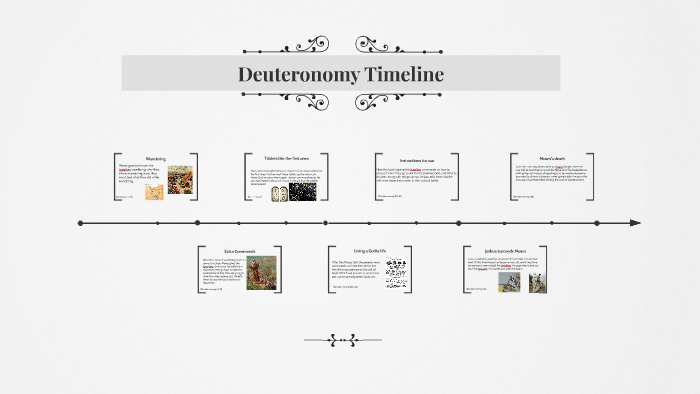
\includegraphics[scale=.7, angle=0]{05OT-Deuteronomy/References/AndrewSmithDeuteronomyTimeline.png}
%\caption[Deuteronomy Timeline by Andrew Smith]{Deuteronomy Timeline by Andrew %Smith}
%\label{fig:Deuteronomy Timeline by Andrew Smith}
%\end{center}
%\end{figure}

\newpage
\begin{figure}
\begin{center}
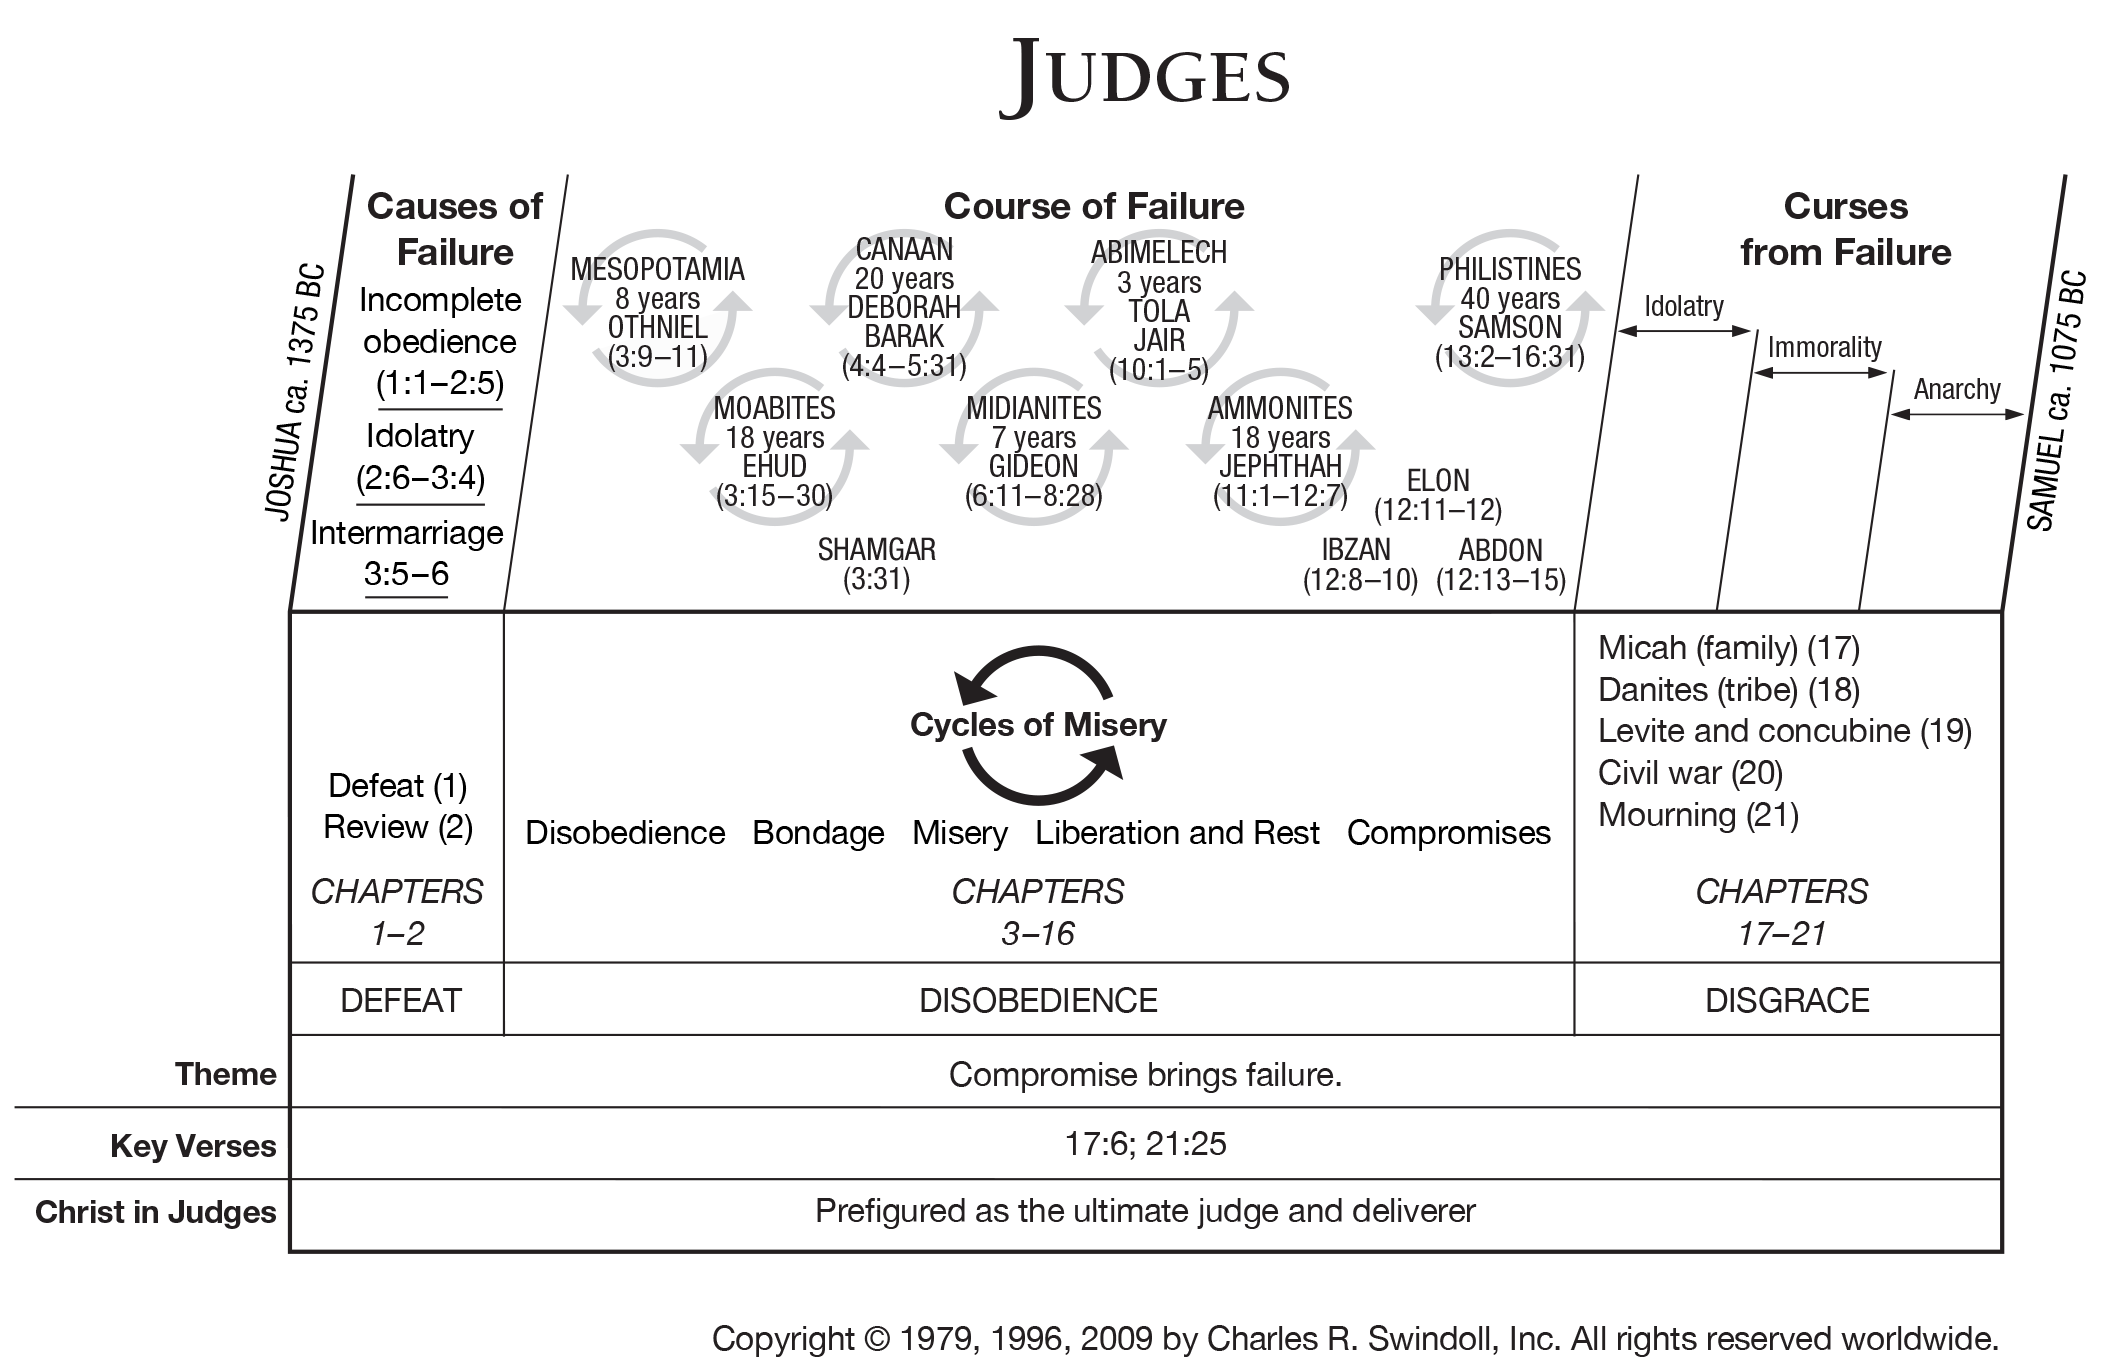
\includegraphics[scale=0.25, angle=90]{07OT-Judges/References/1.Judges-Swindoll}
\caption[Judges from Swindoll]{Judges from Swindoll}
\label{fig:Judges from Swindoll}
\end{center}
\end{figure}


%\newpage
%\begin{figure}
%\begin{center}
%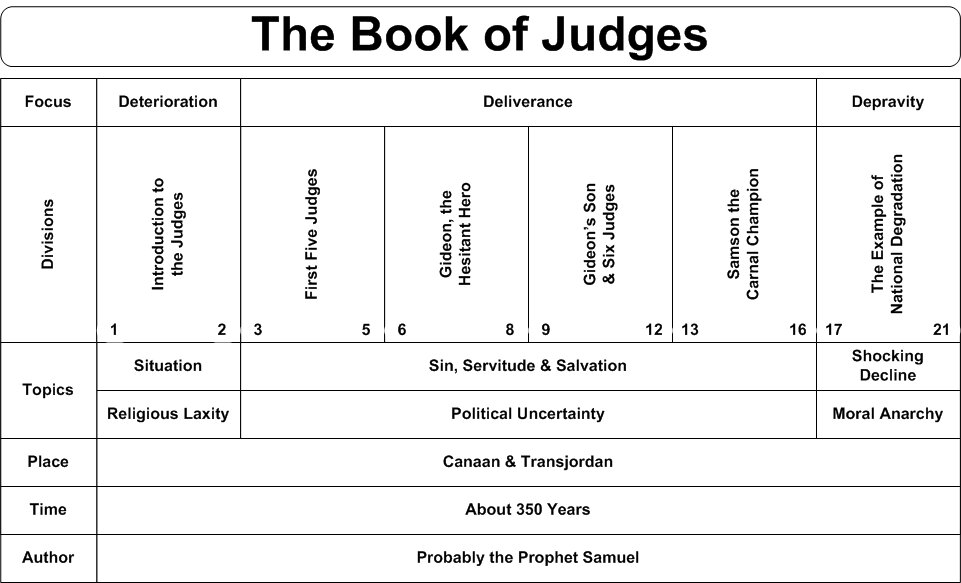
\includegraphics[scale=0.1, angle=0]{07OT-Judges/References/9.Swartzentrover-Judges}
%\caption[Judges from Swartzentrover]{Judges from Swartzentrover}
%\label{fig:Judges from Swartzentrover}
%\end{center}
%\end{figure}


\newpage
\begin{figure}
\begin{center}
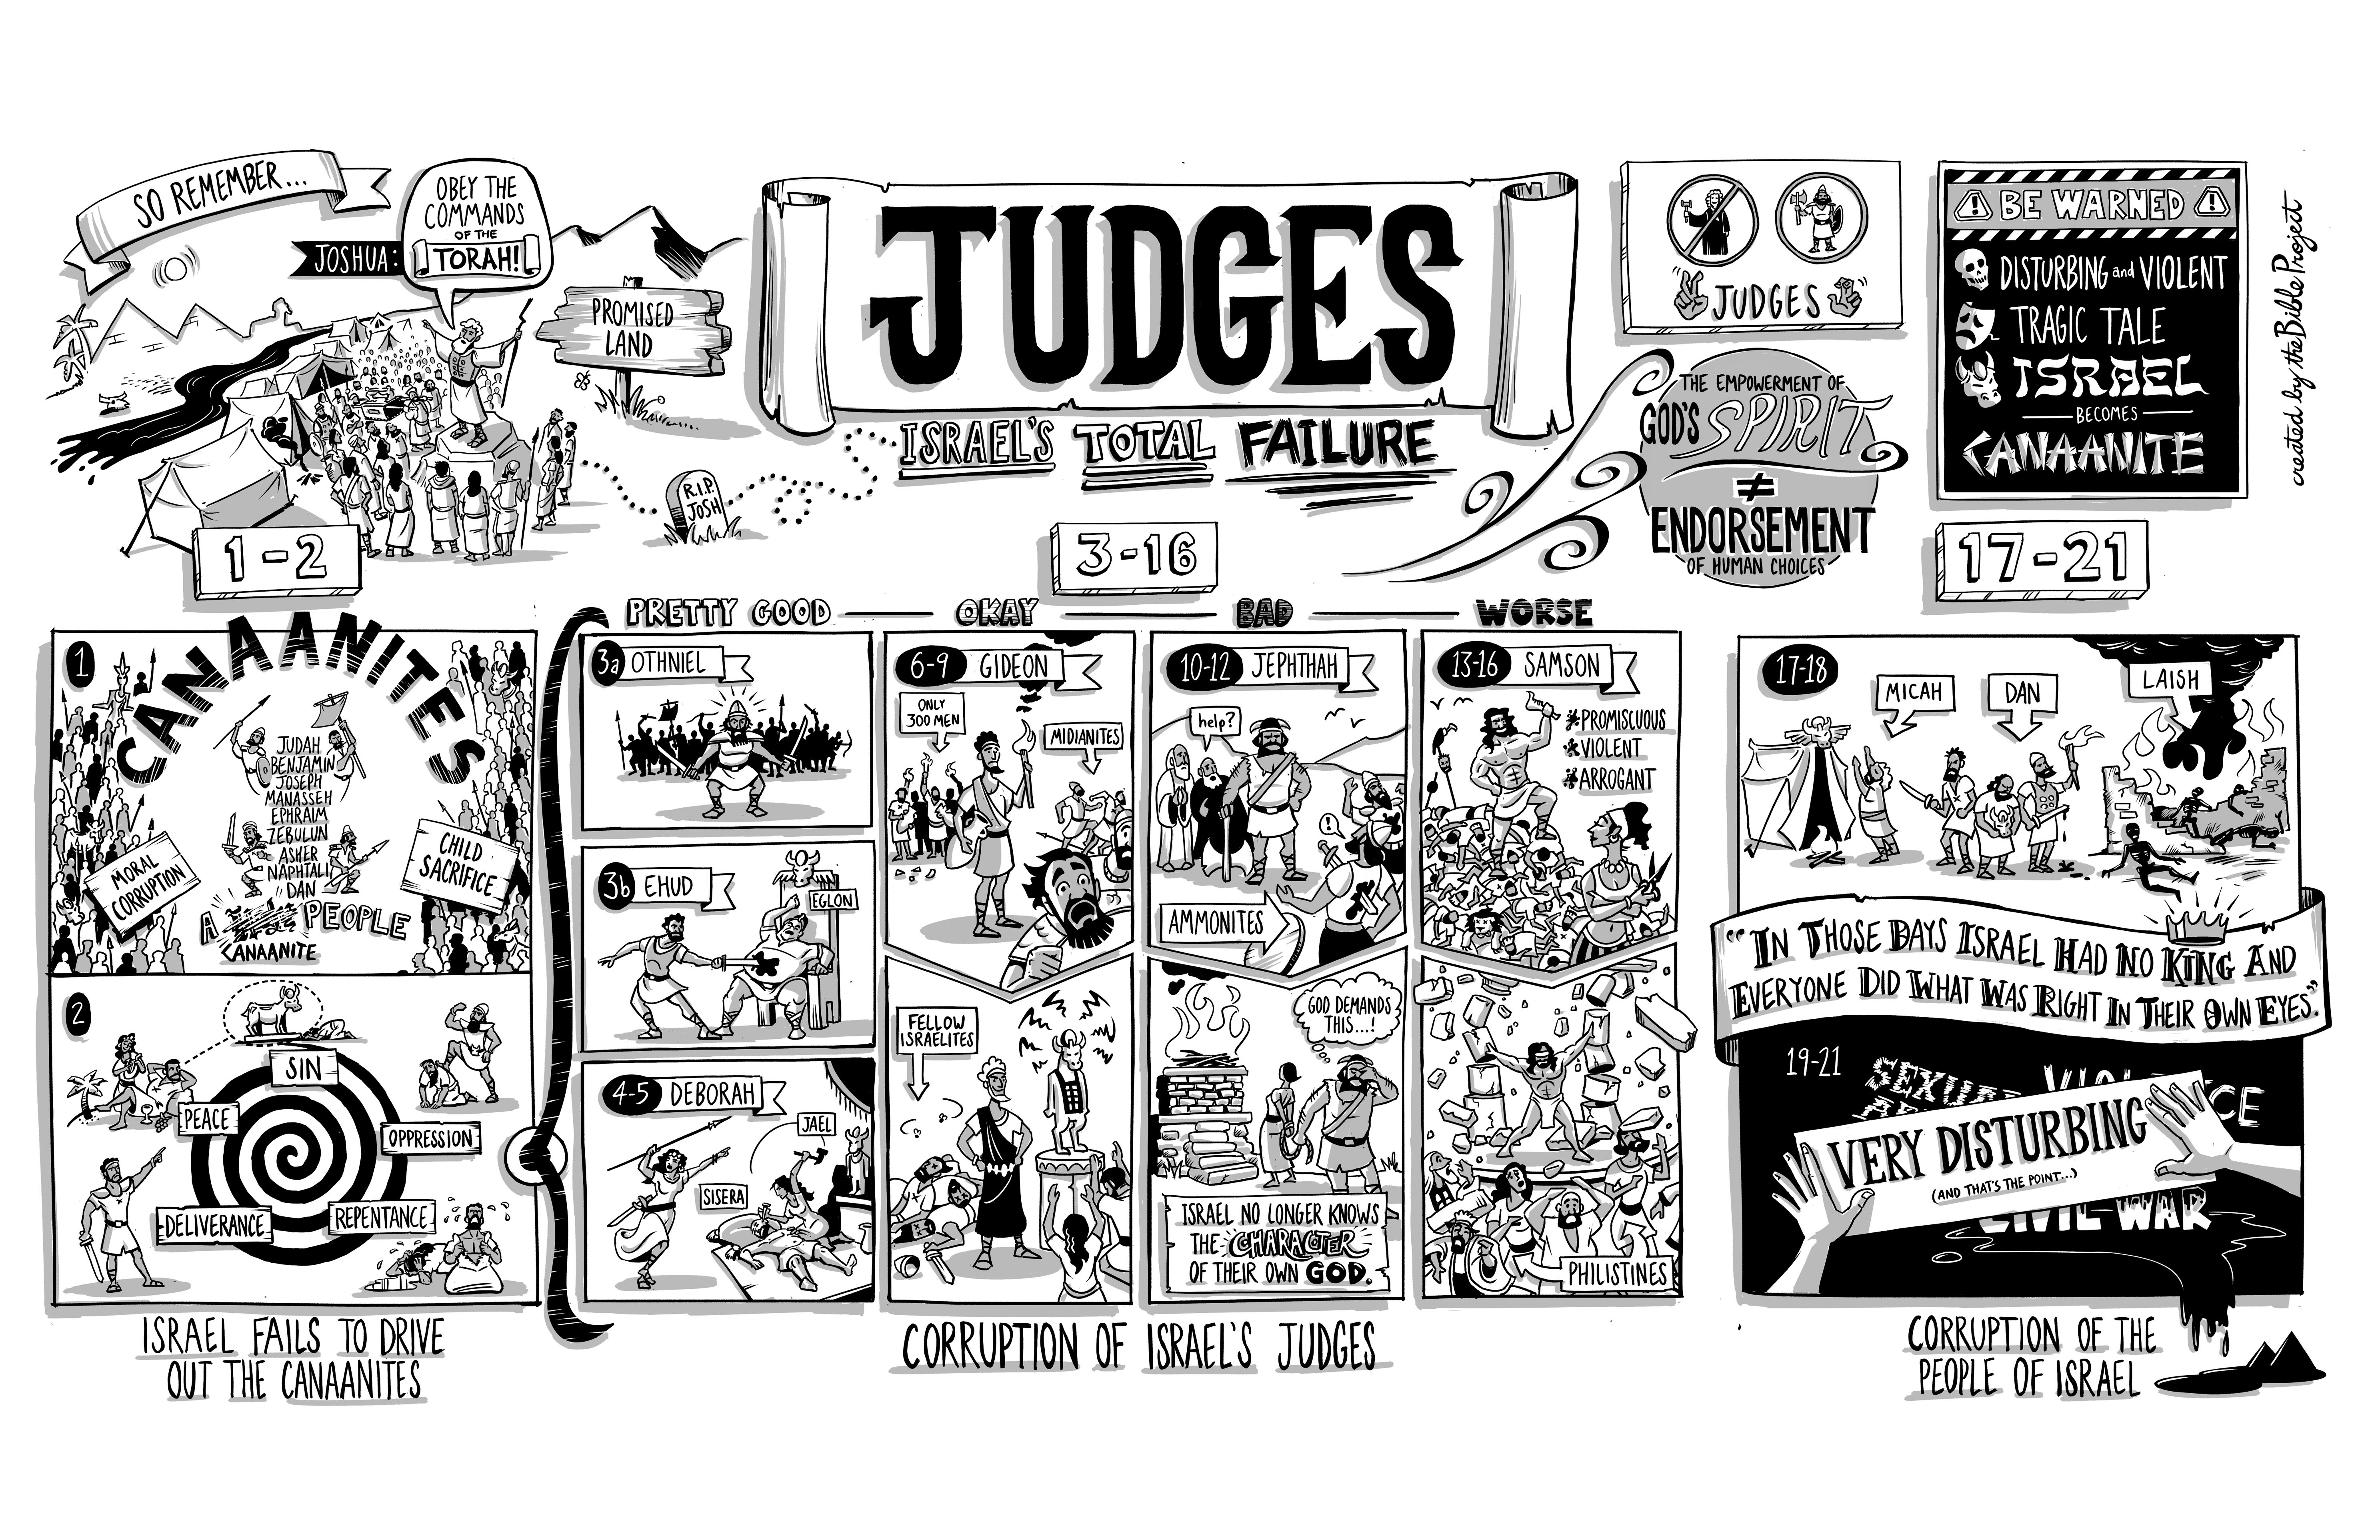
\includegraphics[scale=0.5, angle=90]{07OT-Judges/References/2.BibleProject-Judges}
\caption[Judges from the Bible Project]{Judges from the Bible Project}
\label{fig:Judges from the Bible Project}
\end{center}
\end{figure}


\newpage
\begin{figure}
\begin{center}
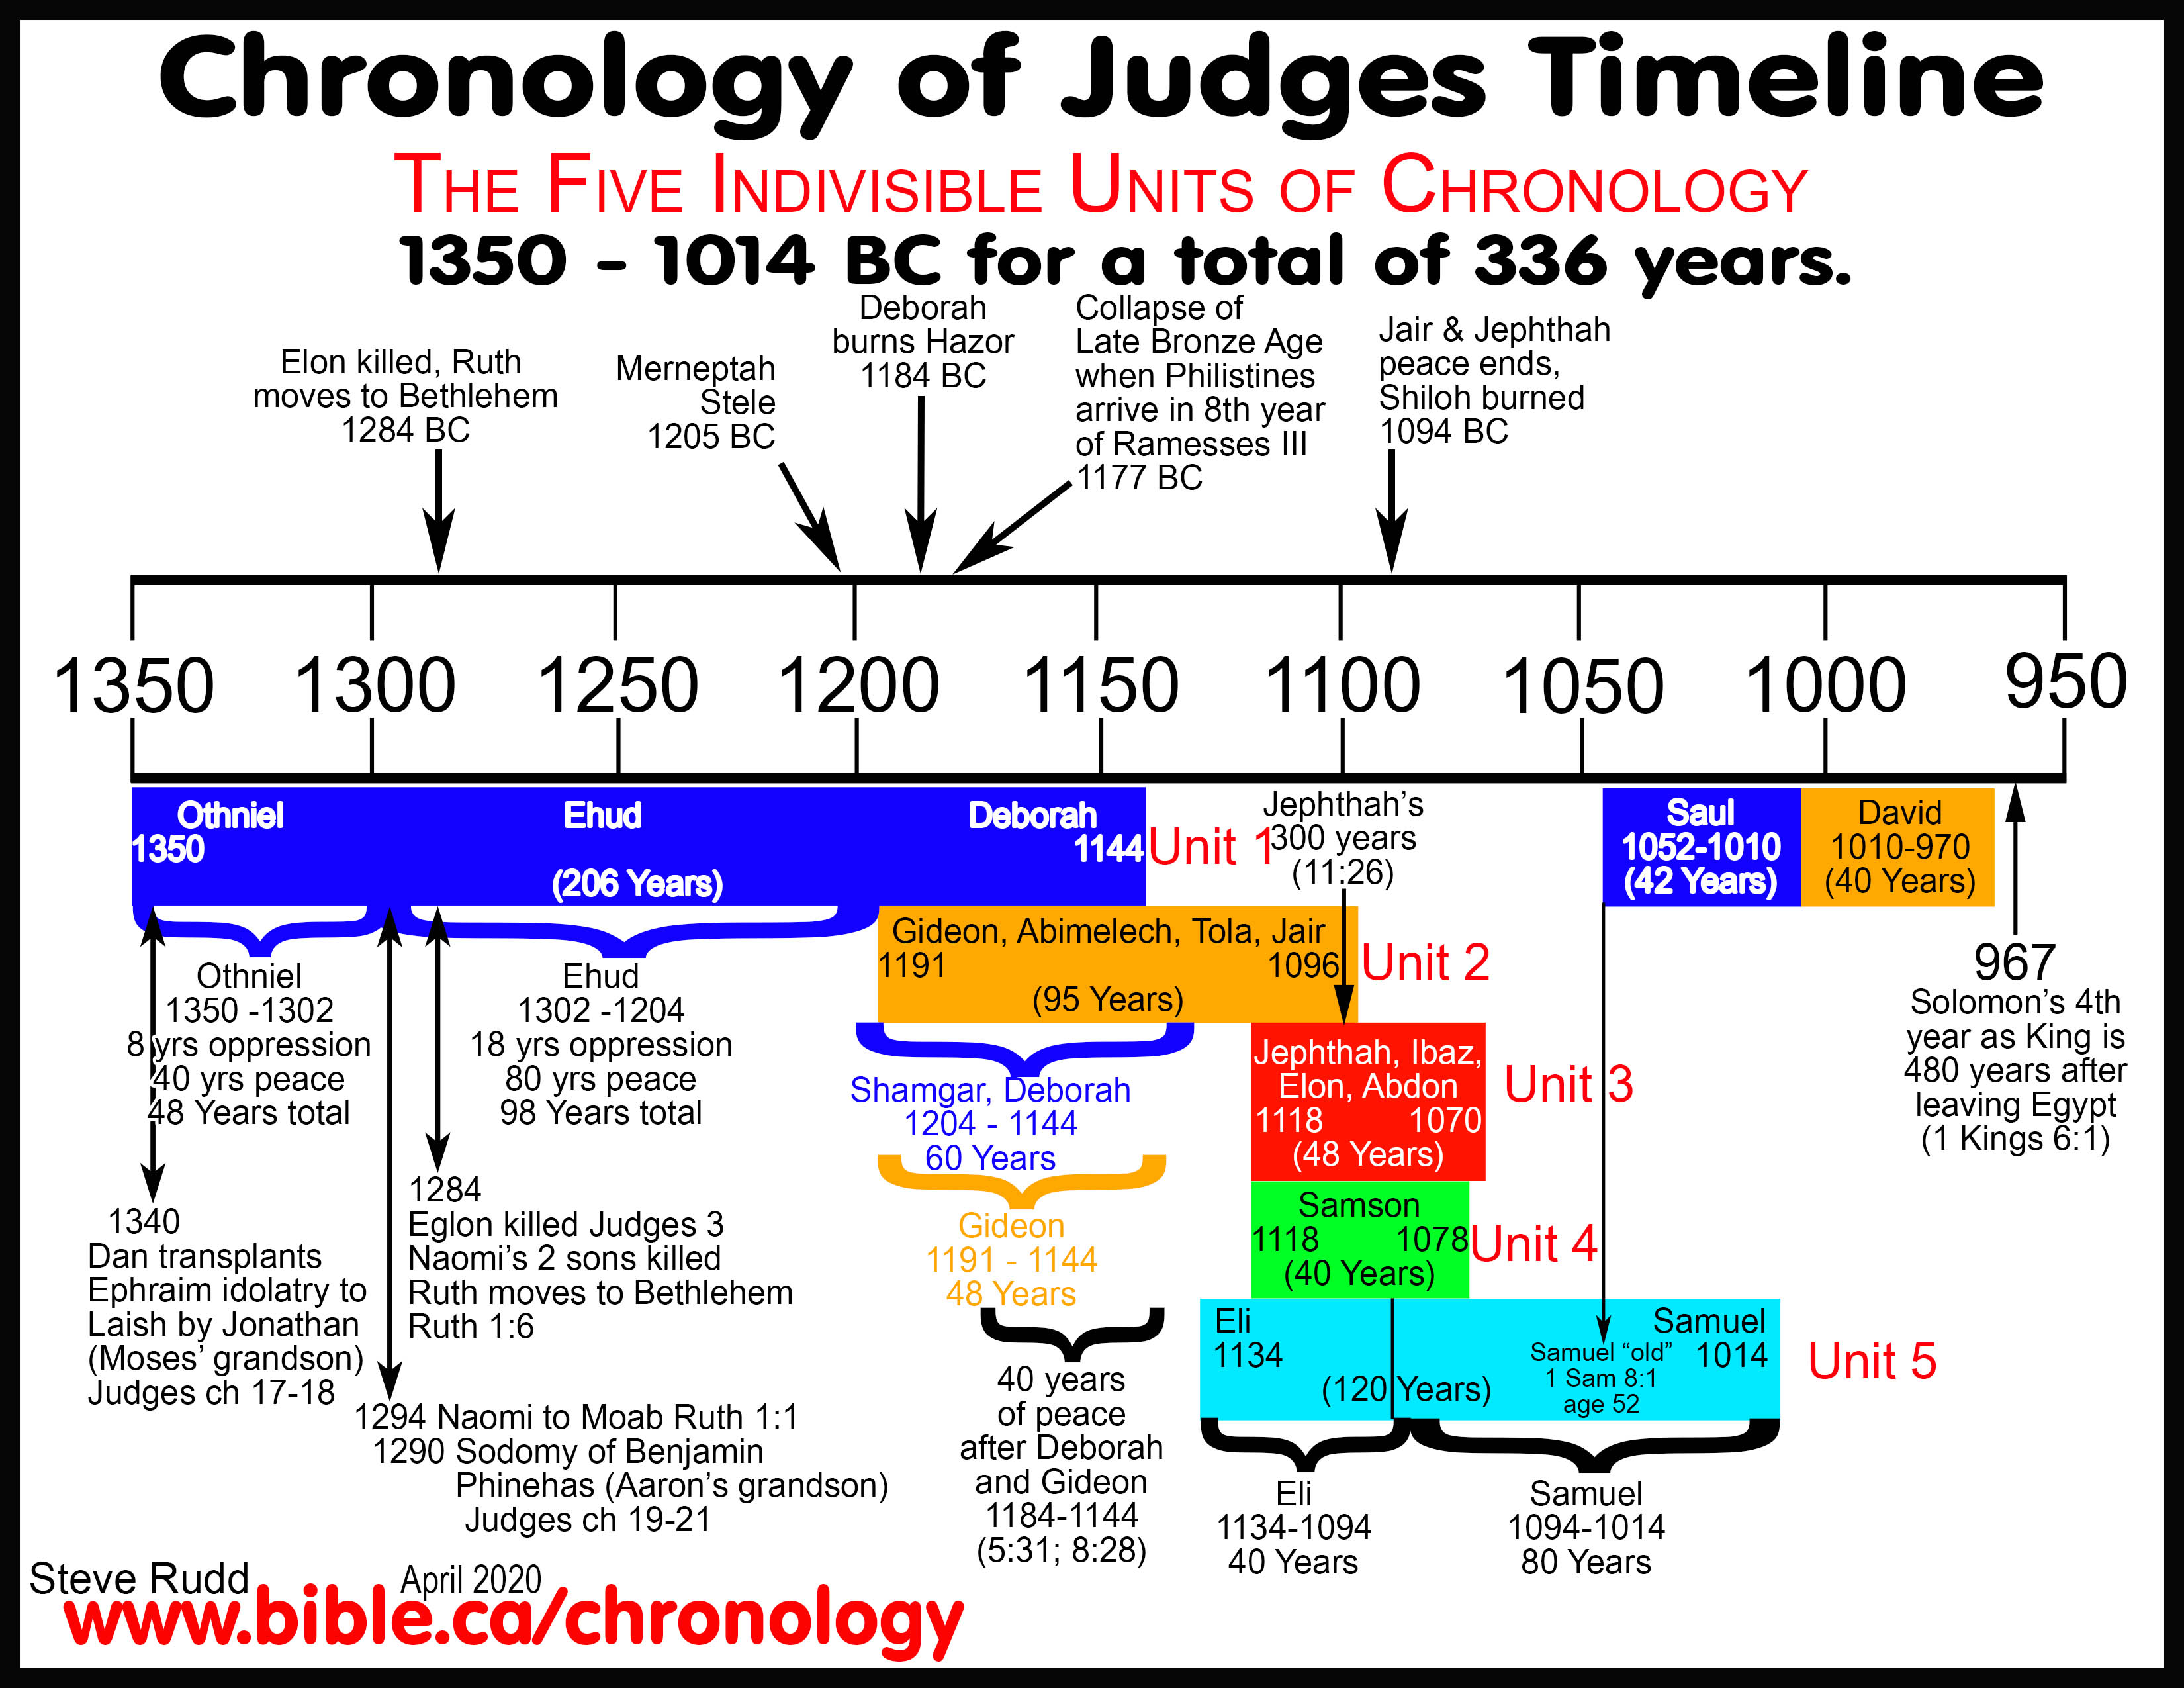
\includegraphics[scale=0.6, angle=90]{07OT-Judges/References/3.Chronology-Judges}
\caption[Chronology of Judges]{Chronology of Judges}
\label{fig:Chronology of Judges}
\end{center}
\end{figure}


\newpage
\begin{figure}
\begin{center}
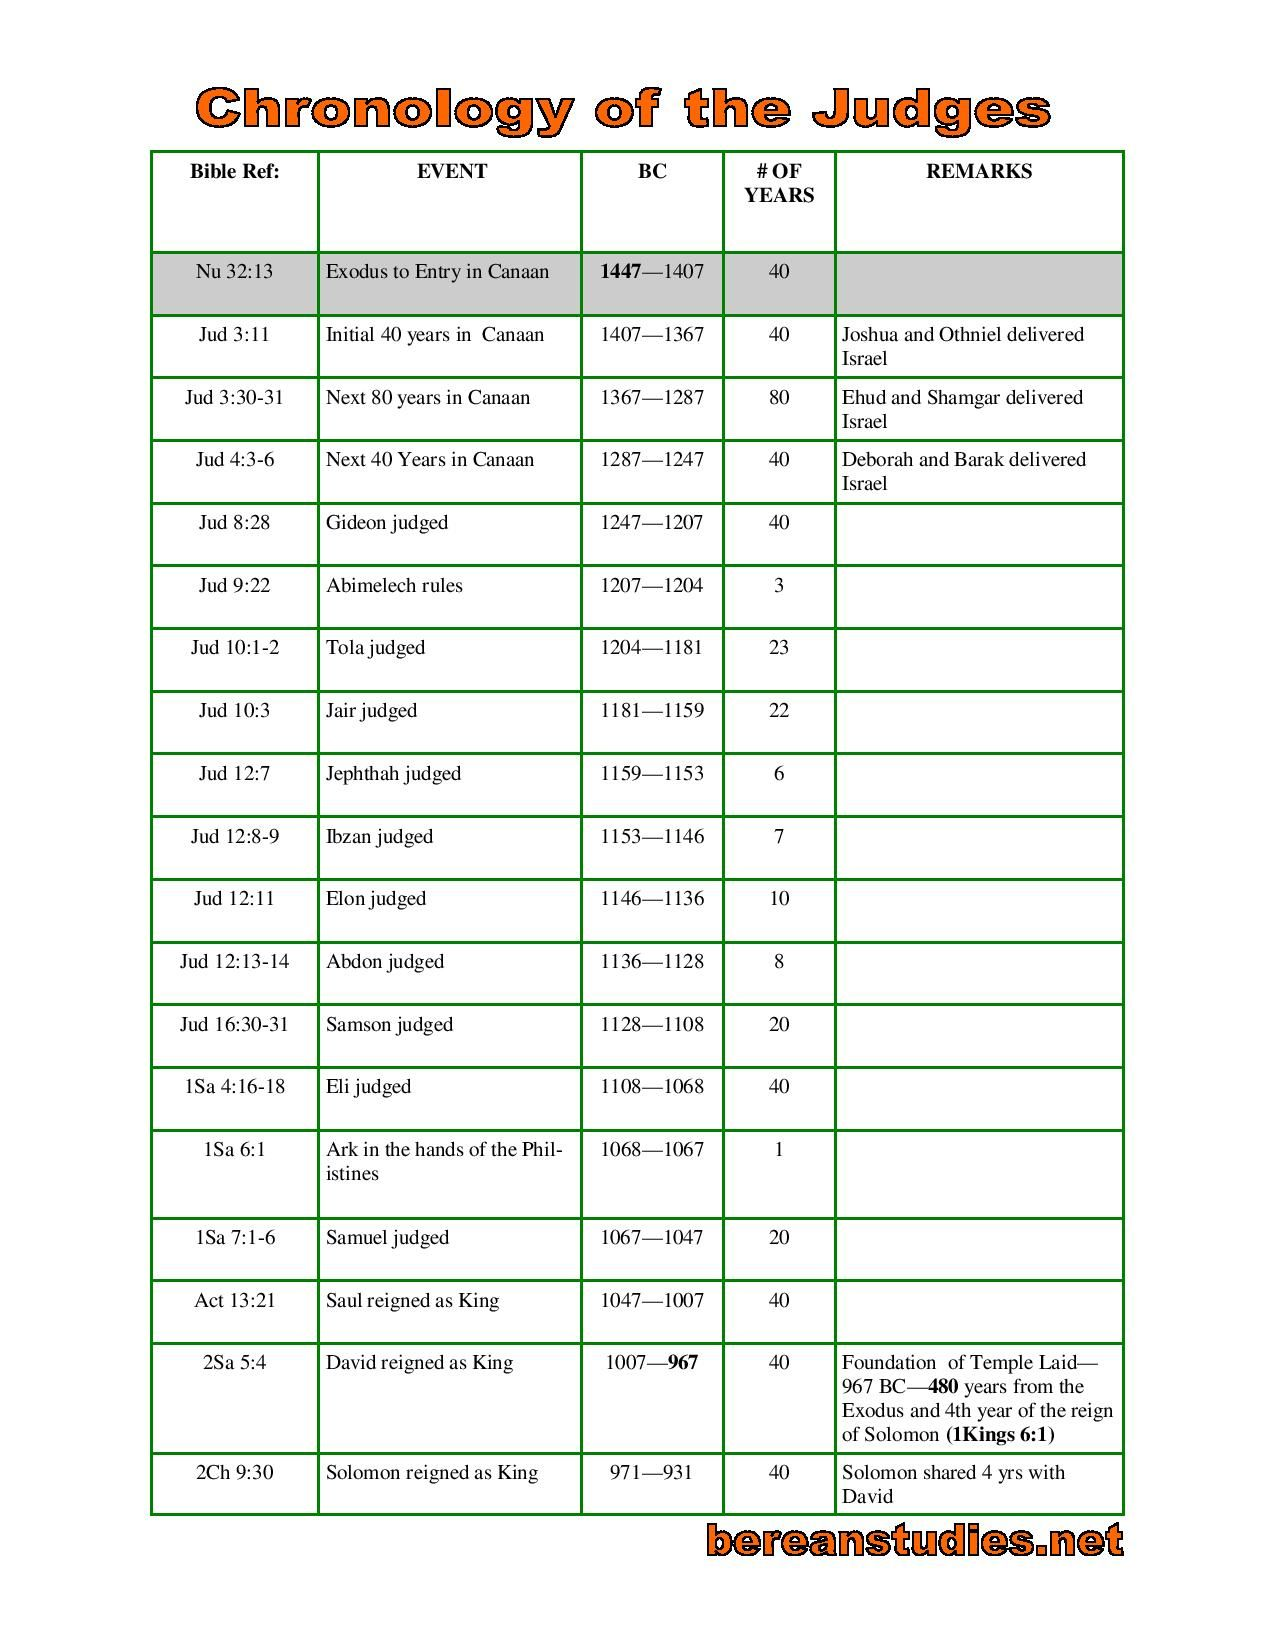
\includegraphics[scale=0.6, angle=0]{07OT-Judges/References/4.Chronology2-Judges}
\caption[Another Chronology of Judges]{Another Chronology of Judges}
\label{fig:Another Chronology of Judges}
\end{center}
\end{figure}

\newpage
\begin{figure}
\begin{center}
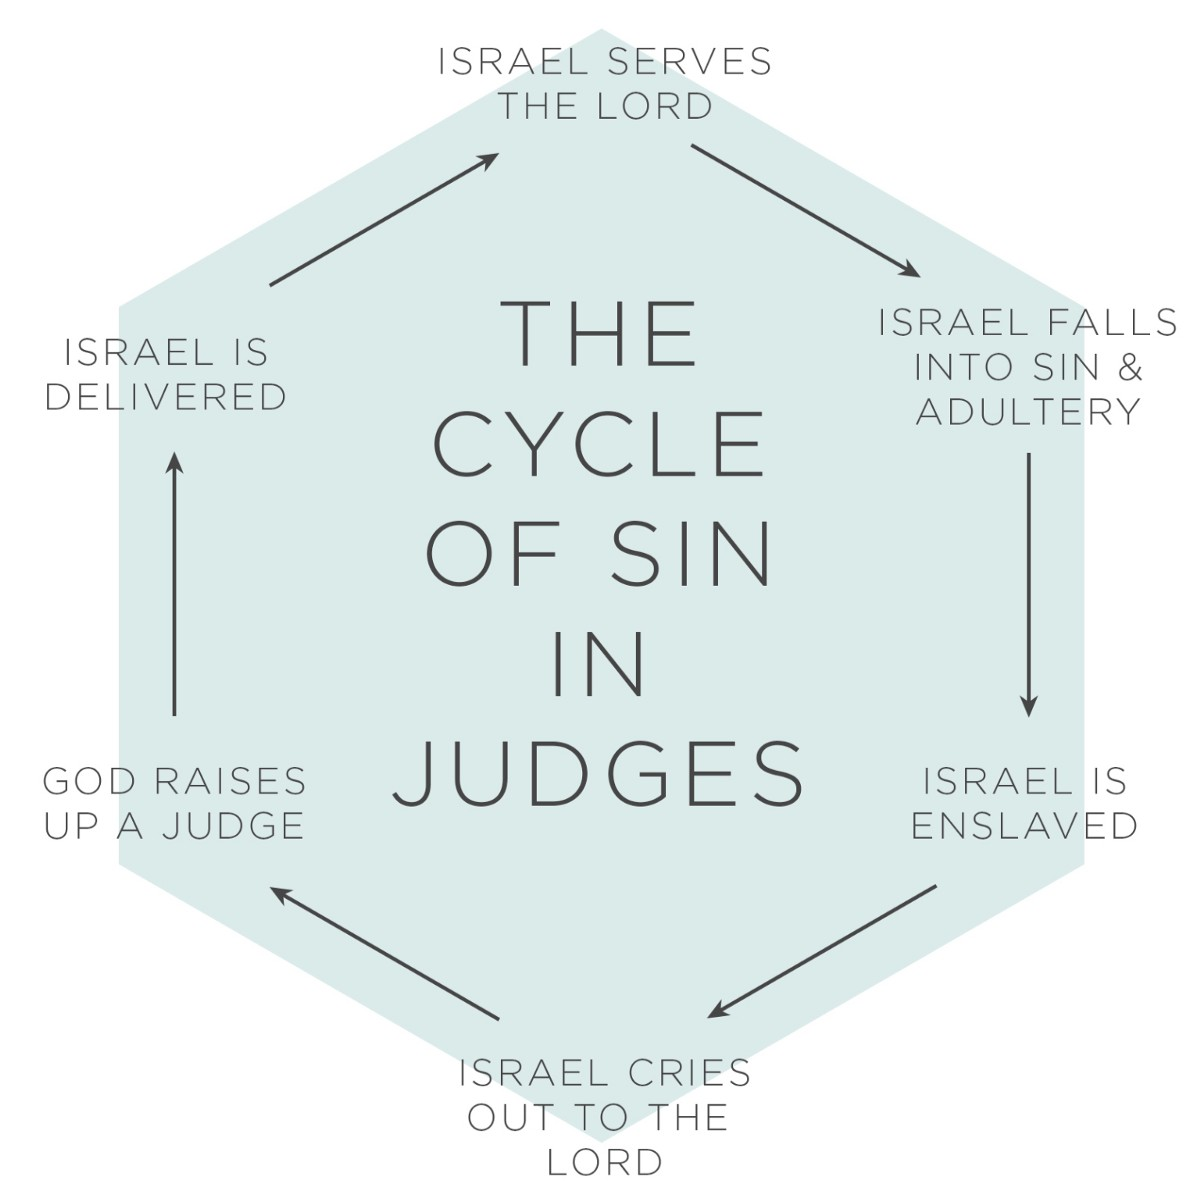
\includegraphics[scale=0.3, angle=0]{07OT-Judges/References/5.Cycles-Judges}
\caption[Cycle of Judges]{Cycle of Judges}
\label{fig:Cycle of Judges}
\end{center}
\end{figure}


\newpage
\begin{figure}
\begin{center}
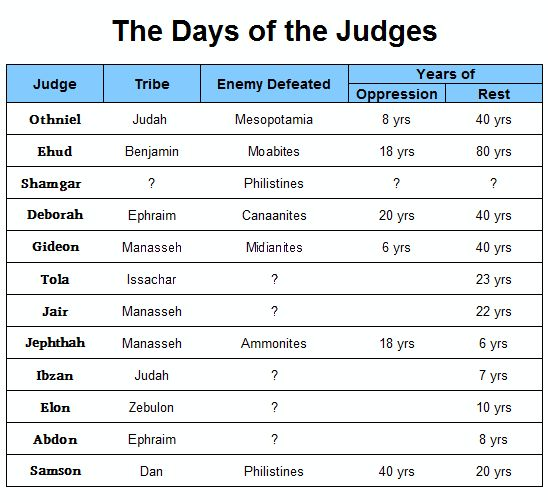
\includegraphics[scale=0.7, angle=0]{07OT-Judges/References/6.DaysOfJudges}
\caption[The Days of the Judges]{The Days of the Judges}
\label{fig:The Days of the Judges}
\end{center}
\end{figure}


\newpage
\begin{figure}
\begin{center}
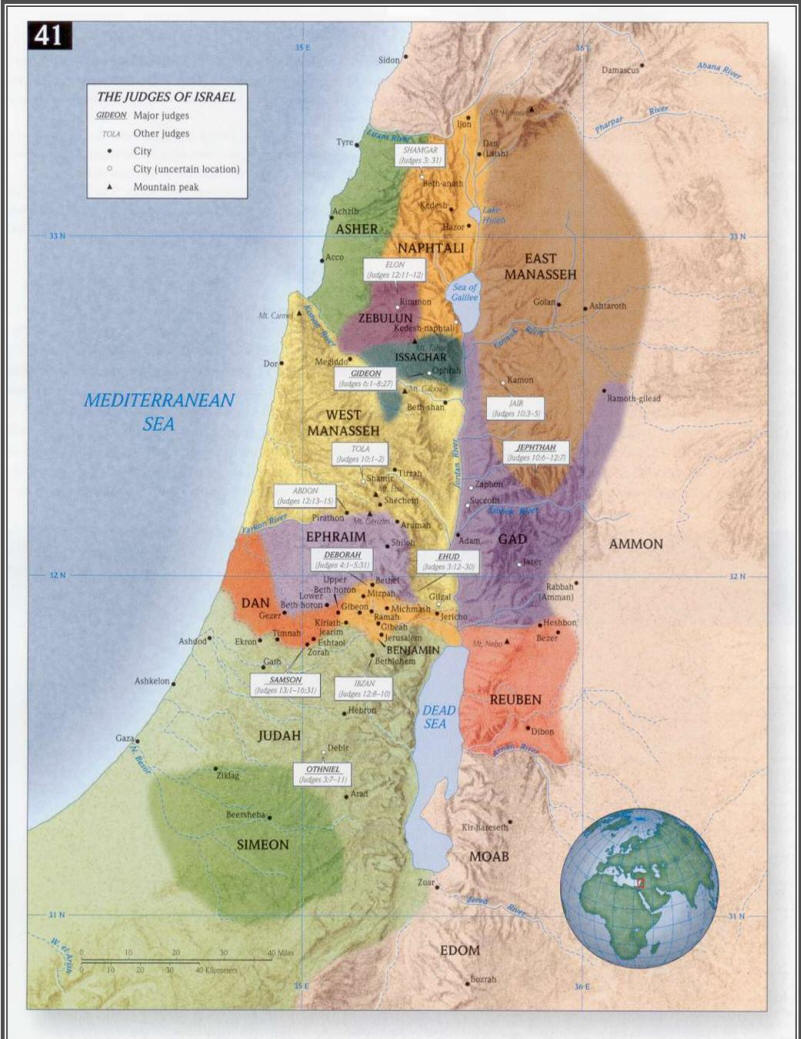
\includegraphics[scale=0.8, angle=0]{07OT-Judges/References/7.Map-Judges}
\caption[Map of the Judges]{Map of the Judges}
\label{fig:Map of the Judges}
\end{center}
\end{figure}


\newpage
\begin{figure}
\begin{center}
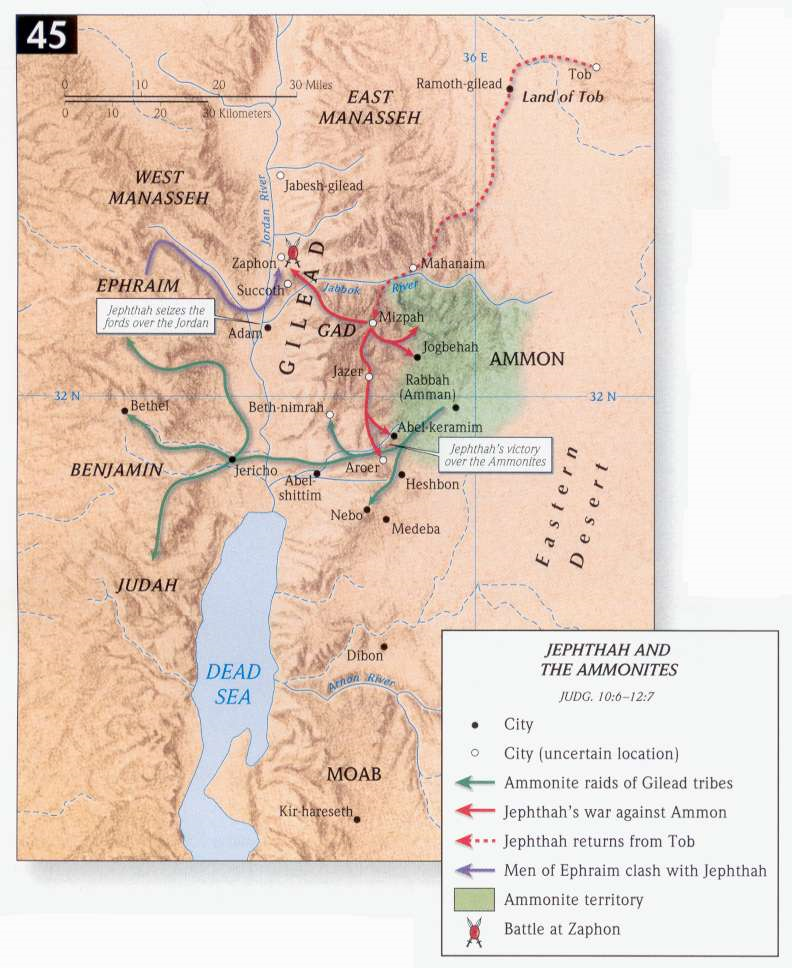
\includegraphics[scale=0.6, angle=0]{07OT-Judges/References/8.Jephthah-Map}
\caption[Map of Jephthah]{Map of Jephthah}
\label{fig:Map of Jephthah}
\end{center}
\end{figure}


\newpage
\begin{figure}
\begin{center}
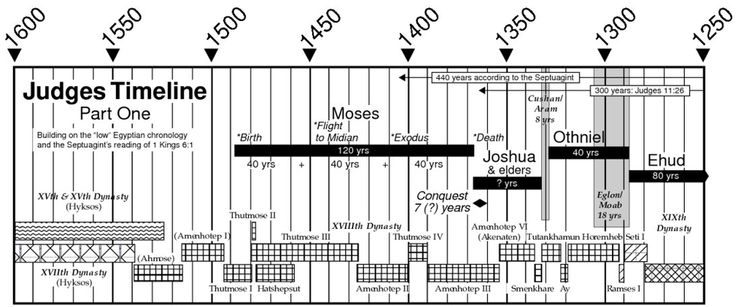
\includegraphics[scale=0.8, angle=90]{07OT-Judges/References/10.Timeline1-Judges}
\caption[Timeline of Judges]{Timeline of Judges}
\label{fig:Timeline of Judges}
\end{center}
\end{figure}



\newpage
\begin{figure}
\begin{center}
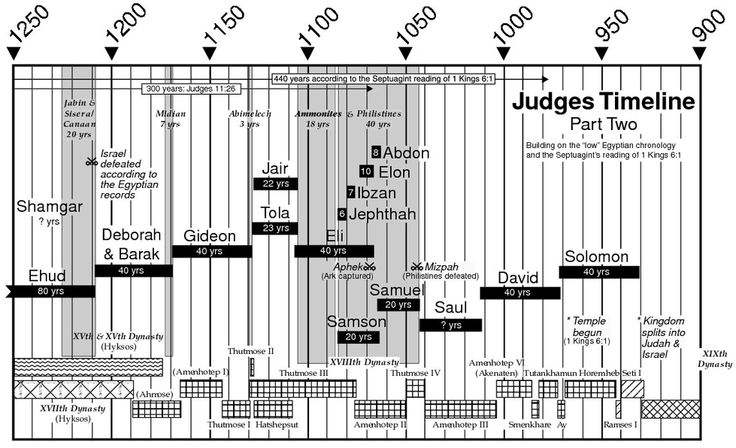
\includegraphics[scale=0.6, angle=90]{07OT-Judges/References/11.Timeline2-Judges}
\caption[Timeline2 of Judges]{Timeline2 of Judges}
\label{fig:Timeline2 of Judges}
\end{center}
\end{figure}


\newpage
\begin{figure}
\begin{center}
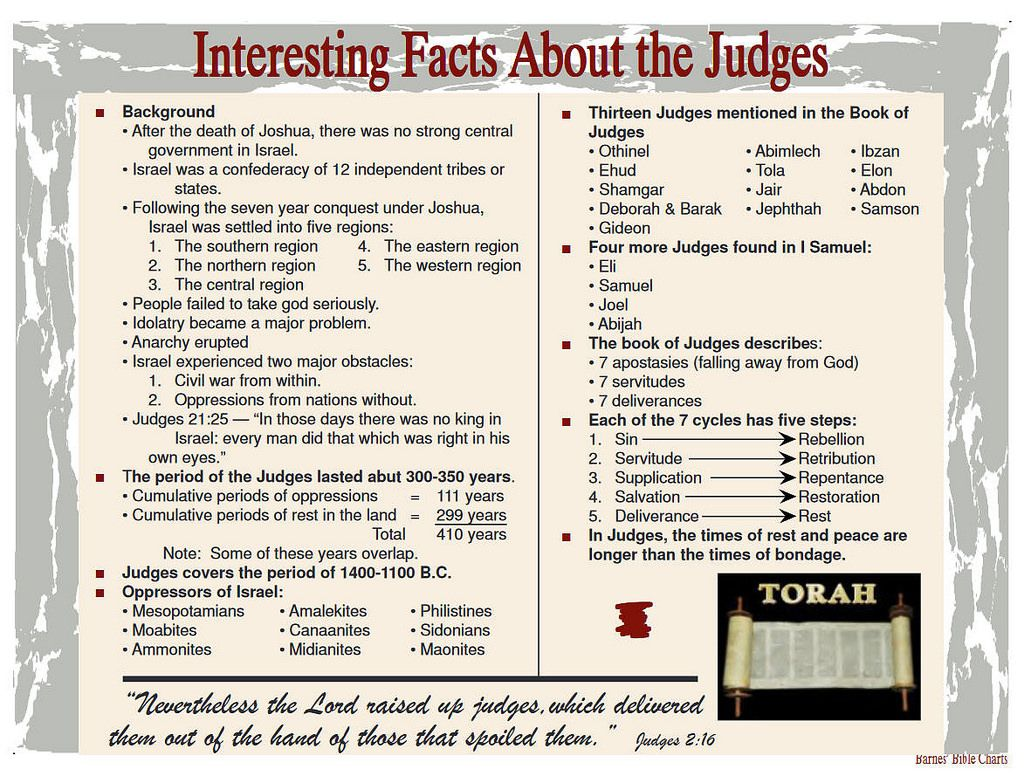
\includegraphics[scale=0.6, angle=90]{07OT-Judges/References/14.InterestingFactsonJudges}
\caption[Interesting Facts about Judges]{Interesting Facts about Judges}
\label{fig:Interesting Facts about Judges}
\end{center}
\end{figure}



\chapter{Judges 13}
 %  \textcolor[cmyk]{0.99998,1,0,0}{

\marginpar{\scriptsize \centering \fcolorbox{bone}{lime}{HELLO SAMSON}\\ (Judges 13) \begin{compactenum}[I.][8]
    \item  The \textbf{Mess} \index[scripture]{Judges!Judges 13:01} (Jdg 13:1) 
    \item  The \textbf{Mother} \index[scripture]{Judges!Judges 13:03} (Jdg 13:3) 
    \item  The \textbf{Messenger} \index[scripture]{Judges!Judges 13:03}(Jdg 13:3)
    \item  The \textbf{Manner} \index[scripture]{Judges!Judges 13:05}(Jdg 13:5) 
    \item  The \textbf{Mission} \index[scripture]{Judges!Judges 13:05}(Jdg 13:5) 
    \item  The \textbf{Meat} Offering \index[scripture]{Judges!Judges 13:10}(Jdg 13:19)
    \item  The \textbf{Moving}  \index[scripture]{Judges!Judges 13:25}(Jdg 13:25)
\end{compactenum}}


\footnote{\textcolor[rgb]{0.00,0.25,0.00}{\hyperlink{JudgesTOC}{Return to end of Table of Contents.}}}\footnote{\href{https://audiobible.com/bible/judges_13.html}{\textcolor[cmyk]{0.99998,1,0,0}{Judges 13 Audio}}}\textcolor[cmyk]{0.99998,1,0,0}{And the children of Israel did evil again in the sight of the LORD; and the LORD delivered them into the hand of the Philistines forty years.}
[2] \textcolor[cmyk]{0.99998,1,0,0}{And there was a certain man of Zorah, of the family of the Danites, whose name \emph{was} Manoah; and his wife \emph{was} barren, and bare not.}
[3] \textcolor[cmyk]{0.99998,1,0,0}{And the angel of the LORD appeared unto the woman, and said unto her, Behold now, thou \emph{art} barren, and bearest not: but thou shalt conceive, and bear a son.}
[4] \textcolor[cmyk]{0.99998,1,0,0}{Now therefore beware, I pray thee, and drink not wine nor strong drink, and eat not any unclean \emph{thing}:}
[5] \textcolor[cmyk]{0.99998,1,0,0}{For, lo, thou shalt conceive, and bear a son; and no razor shall come on his head: for the child shall be a Nazarite unto God from the womb: and he shall begin \fcolorbox{bone}{bone}{to} deliver Israel out of the hand of the Philistines.}\\
\\
\P \textcolor[cmyk]{0.99998,1,0,0}{Then the woman came and told her husband, saying, A man of God came unto me, and his countenance \emph{was} like the countenance of an angel of God, very terrible: but I asked him not whence he \emph{was}, neither told he me his name:}
[7] \textcolor[cmyk]{0.99998,1,0,0}{But he said unto me, Behold, thou shalt conceive, and bear a son; and now drink no wine nor strong drink, neither eat any unclean \emph{thing}: for the child shall be a Nazarite \fcolorbox{bone}{bone}{to} God from the womb \fcolorbox{bone}{bone}{to} the day of his death.}\\
\\
\P \textcolor[cmyk]{0.99998,1,0,0}{Then Manoah intreated the LORD, and said, O my Lord, let the man of God which thou didst send come again unto us, and teach us what we shall do unto the child that shall be born.}
[9] \textcolor[cmyk]{0.99998,1,0,0}{And God hearkened \fcolorbox{bone}{bone}{to} the voice of Manoah; and the angel of God came again unto the woman as she sat in the field: but Manoah her husband \emph{was} not with her.}
[10] \textcolor[cmyk]{0.99998,1,0,0}{And the woman made haste, and ran, and shewed her husband, and said unto him, Behold, the man hath appeared unto me, that came unto me the \emph{other} day.}
[11] \textcolor[cmyk]{0.99998,1,0,0}{And Manoah arose, and went after his wife, and came \fcolorbox{bone}{bone}{to} the man, and said unto him, \emph{Art} thou the man that spakest unto the woman? And he said, I \emph{am}.}
[12] \textcolor[cmyk]{0.99998,1,0,0}{And Manoah said, Now let thy words come \fcolorbox{bone}{bone}{to} pass. How shall we order the child, and \emph{how} shall we do unto him?}
[13] \textcolor[cmyk]{0.99998,1,0,0}{And the angel of the LORD said unto Manoah, Of all that I said unto the woman let her beware.}
[14] \textcolor[cmyk]{0.99998,1,0,0}{She may not eat of any \emph{thing} that cometh of the vine, neither let her drink wine or strong drink, nor eat any unclean \emph{thing}: all that I commanded her let her observe.}\\
\\
\P \textcolor[cmyk]{0.99998,1,0,0}{And Manoah said unto the angel of the LORD, I pray thee, let us detain thee, until we shall have made ready a kid for thee.}
[16] \textcolor[cmyk]{0.99998,1,0,0}{And the angel of the LORD said unto Manoah, Though thou detain me, I will not eat of thy bread: and if thou wilt offer a burnt offering, thou must offer it unto the LORD. For Manoah knew not that he \emph{was} an angel of the LORD.}
[17] \textcolor[cmyk]{0.99998,1,0,0}{And Manoah said unto the angel of the LORD, What \emph{is} thy name, that when thy sayings come \fcolorbox{bone}{bone}{to} pass we may do thee honour?}
[18] \textcolor[cmyk]{0.99998,1,0,0}{And the angel of the LORD said unto him, Why askest thou thus after my name, seeing it \emph{is} secret?}
[19] \textcolor[cmyk]{0.99998,1,0,0}{So Manoah took a kid with a meat offering, and offered \emph{it} upon a rock unto the LORD: and \emph{the} \emph{angel} did wondrously; and Manoah and his wife looked on.}
[20] \textcolor[cmyk]{0.99998,1,0,0}{For it came \fcolorbox{bone}{bone}{to} pass, when the flame went up toward heaven from off the altar, that the angel of the LORD ascended in the flame of the altar. And Manoah and his wife looked on \emph{it}, and fell on their faces \fcolorbox{bone}{bone}{to} the ground.}
[21] \textcolor[cmyk]{0.99998,1,0,0}{But the angel of the LORD did no more appear \fcolorbox{bone}{bone}{to} Manoah and \fcolorbox{bone}{bone}{to} his wife. Then Manoah knew that he \emph{was} an angel of the LORD.}
[22] \textcolor[cmyk]{0.99998,1,0,0}{And Manoah said unto his wife, We shall surely die, because we have seen God.}
[23] \textcolor[cmyk]{0.99998,1,0,0}{But his wife said unto him, If the LORD were pleased \fcolorbox{bone}{bone}{to} kill us, he would not have received a burnt offering and a meat offering at our hands, neither would he have shewed us all these \emph{things}, nor would as at this time have told us \emph{such} \emph{things} as these.}\\
\\
\P \textcolor[cmyk]{0.99998,1,0,0}{And the woman bare a son, and called his name Samson: and the child grew, and the LORD blessed him.}
[25] \textcolor[cmyk]{0.99998,1,0,0}{And the Spirit of the LORD began \fcolorbox{bone}{bone}{to} move him at times in the camp of Dan between Zorah and Eshtaol.}
\index[NWIV]{27!Judges!Jud 13:1}\index[AWIP]{And!Judges!Jud 13:1}\index[AWIP]{the!Judges!Jud 13:1}\index[AWIP]{the!Judges!Jud 13:1 (2)}\index[AWIP]{the!Judges!Jud 13:1 (3)}\index[AWIP]{the!Judges!Jud 13:1 (4)}\index[AWIP]{the!Judges!Jud 13:1 (5)}\index[AWIP]{the!Judges!Jud 13:1 (6)}\index[AWIP]{children!Judges!Jud 13:1}\index[AWIP]{of!Judges!Jud 13:1}\index[AWIP]{of!Judges!Jud 13:1 (2)}\index[AWIP]{of!Judges!Jud 13:1 (3)}\index[AWIP]{Israel!Judges!Jud 13:1}\index[AWIP]{did!Judges!Jud 13:1}\index[AWIP]{evil!Judges!Jud 13:1}\index[AWIP]{again!Judges!Jud 13:1}\index[AWIP]{in!Judges!Jud 13:1}\index[AWIP]{sight!Judges!Jud 13:1}\index[AWIP]{LORD!Judges!Jud 13:1}\index[AWIP]{LORD!Judges!Jud 13:1 (2)}\index[AWIP]{and!Judges!Jud 13:1}\index[AWIP]{delivered!Judges!Jud 13:1}\index[AWIP]{them!Judges!Jud 13:1}\index[AWIP]{into!Judges!Jud 13:1}\index[AWIP]{hand!Judges!Jud 13:1}\index[AWIP]{Philistines!Judges!Jud 13:1}\index[AWIP]{forty!Judges!Jud 13:1}\index[AWIP]{years!Judges!Jud 13:1}

\index[NWIV]{26!Judges!Jud 13:2}\index[AWIP]{And!Judges!Jud 13:2}\index[AWIP]{there!Judges!Jud 13:2}\index[AWIP]{was!Judges!Jud 13:2}\index[AWIP]{a!Judges!Jud 13:2}\index[AWIP]{certain!Judges!Jud 13:2}\index[AWIP]{man!Judges!Jud 13:2}\index[AWIP]{of!Judges!Jud 13:2}\index[AWIP]{of!Judges!Jud 13:2 (2)}\index[AWIP]{of!Judges!Jud 13:2 (3)}\index[AWIP]{Zorah!Judges!Jud 13:2}\index[AWIP]{the!Judges!Jud 13:2}\index[AWIP]{the!Judges!Jud 13:2 (2)}\index[AWIP]{family!Judges!Jud 13:2}\index[AWIP]{Danites!Judges!Jud 13:2}\index[AWIP]{whose!Judges!Jud 13:2}\index[AWIP]{name!Judges!Jud 13:2}\index[AWIP]{\emph{was}!Judges!Jud 13:2}\index[AWIP]{\emph{was}!Judges!Jud 13:2 (2)}\index[AWIP]{Manoah!Judges!Jud 13:2}\index[AWIP]{and!Judges!Jud 13:2}\index[AWIP]{and!Judges!Jud 13:2 (2)}\index[AWIP]{his!Judges!Jud 13:2}\index[AWIP]{wife!Judges!Jud 13:2}\index[AWIP]{barren!Judges!Jud 13:2}\index[AWIP]{bare!Judges!Jud 13:2}\index[AWIP]{not!Judges!Jud 13:2}\index[AWIP]{\emph{was}!Judges!Jud 13:2}\index[AWIP]{\emph{was}!Judges!Jud 13:2 (2)}

\index[NWIV]{30!Judges!Jud 13:3}\index[AWIP]{And!Judges!Jud 13:3}\index[AWIP]{the!Judges!Jud 13:3}\index[AWIP]{the!Judges!Jud 13:3 (2)}\index[AWIP]{the!Judges!Jud 13:3 (3)}\index[AWIP]{angel!Judges!Jud 13:3}\index[AWIP]{of!Judges!Jud 13:3}\index[AWIP]{LORD!Judges!Jud 13:3}\index[AWIP]{appeared!Judges!Jud 13:3}\index[AWIP]{unto!Judges!Jud 13:3}\index[AWIP]{unto!Judges!Jud 13:3 (2)}\index[AWIP]{woman!Judges!Jud 13:3}\index[AWIP]{and!Judges!Jud 13:3}\index[AWIP]{and!Judges!Jud 13:3 (2)}\index[AWIP]{and!Judges!Jud 13:3 (3)}\index[AWIP]{said!Judges!Jud 13:3}\index[AWIP]{her!Judges!Jud 13:3}\index[AWIP]{Behold!Judges!Jud 13:3}\index[AWIP]{now!Judges!Jud 13:3}\index[AWIP]{thou!Judges!Jud 13:3}\index[AWIP]{thou!Judges!Jud 13:3 (2)}\index[AWIP]{\emph{art}!Judges!Jud 13:3}\index[AWIP]{barren!Judges!Jud 13:3}\index[AWIP]{bearest!Judges!Jud 13:3}\index[AWIP]{not!Judges!Jud 13:3}\index[AWIP]{but!Judges!Jud 13:3}\index[AWIP]{shalt!Judges!Jud 13:3}\index[AWIP]{conceive!Judges!Jud 13:3}\index[AWIP]{bear!Judges!Jud 13:3}\index[AWIP]{a!Judges!Jud 13:3}\index[AWIP]{son!Judges!Jud 13:3}\index[AWIP]{\emph{art}!Judges!Jud 13:3}

\index[NWIV]{19!Judges!Jud 13:4}\index[AWIP]{Now!Judges!Jud 13:4}\index[AWIP]{therefore!Judges!Jud 13:4}\index[AWIP]{beware!Judges!Jud 13:4}\index[AWIP]{I!Judges!Jud 13:4}\index[AWIP]{pray!Judges!Jud 13:4}\index[AWIP]{thee!Judges!Jud 13:4}\index[AWIP]{and!Judges!Jud 13:4}\index[AWIP]{and!Judges!Jud 13:4 (2)}\index[AWIP]{drink!Judges!Jud 13:4}\index[AWIP]{drink!Judges!Jud 13:4 (2)}\index[AWIP]{not!Judges!Jud 13:4}\index[AWIP]{not!Judges!Jud 13:4 (2)}\index[AWIP]{wine!Judges!Jud 13:4}\index[AWIP]{nor!Judges!Jud 13:4}\index[AWIP]{strong!Judges!Jud 13:4}\index[AWIP]{eat!Judges!Jud 13:4}\index[AWIP]{any!Judges!Jud 13:4}\index[AWIP]{unclean!Judges!Jud 13:4}\index[AWIP]{\emph{thing}!Judges!Jud 13:4}\index[AWIP]{\emph{thing}!Judges!Jud 13:4}

\index[NWIV]{43!Judges!Jud 13:5}\index[AWIP]{For!Judges!Jud 13:5}\index[AWIP]{lo!Judges!Jud 13:5}\index[AWIP]{thou!Judges!Jud 13:5}\index[AWIP]{shalt!Judges!Jud 13:5}\index[AWIP]{conceive!Judges!Jud 13:5}\index[AWIP]{and!Judges!Jud 13:5}\index[AWIP]{and!Judges!Jud 13:5 (2)}\index[AWIP]{and!Judges!Jud 13:5 (3)}\index[AWIP]{bear!Judges!Jud 13:5}\index[AWIP]{a!Judges!Jud 13:5}\index[AWIP]{a!Judges!Jud 13:5 (2)}\index[AWIP]{son!Judges!Jud 13:5}\index[AWIP]{no!Judges!Jud 13:5}\index[AWIP]{razor!Judges!Jud 13:5}\index[AWIP]{shall!Judges!Jud 13:5}\index[AWIP]{shall!Judges!Jud 13:5 (2)}\index[AWIP]{shall!Judges!Jud 13:5 (3)}\index[AWIP]{come!Judges!Jud 13:5}\index[AWIP]{on!Judges!Jud 13:5}\index[AWIP]{his!Judges!Jud 13:5}\index[AWIP]{head!Judges!Jud 13:5}\index[AWIP]{for!Judges!Jud 13:5}\index[AWIP]{the!Judges!Jud 13:5}\index[AWIP]{the!Judges!Jud 13:5 (2)}\index[AWIP]{the!Judges!Jud 13:5 (3)}\index[AWIP]{the!Judges!Jud 13:5 (4)}\index[AWIP]{child!Judges!Jud 13:5}\index[AWIP]{be!Judges!Jud 13:5}\index[AWIP]{Nazarite!Judges!Jud 13:5}\index[AWIP]{unto!Judges!Jud 13:5}\index[AWIP]{God!Judges!Jud 13:5}\index[AWIP]{from!Judges!Jud 13:5}\index[AWIP]{womb!Judges!Jud 13:5}\index[AWIP]{he!Judges!Jud 13:5}\index[AWIP]{begin!Judges!Jud 13:5}\index[AWIP]{to!Judges!Jud 13:5}\index[AWIP]{deliver!Judges!Jud 13:5}\index[AWIP]{Israel!Judges!Jud 13:5}\index[AWIP]{out!Judges!Jud 13:5}\index[AWIP]{of!Judges!Jud 13:5}\index[AWIP]{of!Judges!Jud 13:5 (2)}\index[AWIP]{hand!Judges!Jud 13:5}\index[AWIP]{Philistines!Judges!Jud 13:5}

\index[NWIV]{44!Judges!Jud 13:6}\index[AWIP]{Then!Judges!Jud 13:6}\index[AWIP]{the!Judges!Jud 13:6}\index[AWIP]{the!Judges!Jud 13:6 (2)}\index[AWIP]{woman!Judges!Jud 13:6}\index[AWIP]{came!Judges!Jud 13:6}\index[AWIP]{came!Judges!Jud 13:6 (2)}\index[AWIP]{and!Judges!Jud 13:6}\index[AWIP]{and!Judges!Jud 13:6 (2)}\index[AWIP]{told!Judges!Jud 13:6}\index[AWIP]{told!Judges!Jud 13:6 (2)}\index[AWIP]{her!Judges!Jud 13:6}\index[AWIP]{husband!Judges!Jud 13:6}\index[AWIP]{saying!Judges!Jud 13:6}\index[AWIP]{A!Judges!Jud 13:6}\index[AWIP]{man!Judges!Jud 13:6}\index[AWIP]{of!Judges!Jud 13:6}\index[AWIP]{of!Judges!Jud 13:6 (2)}\index[AWIP]{of!Judges!Jud 13:6 (3)}\index[AWIP]{God!Judges!Jud 13:6}\index[AWIP]{God!Judges!Jud 13:6 (2)}\index[AWIP]{unto!Judges!Jud 13:6}\index[AWIP]{me!Judges!Jud 13:6}\index[AWIP]{me!Judges!Jud 13:6 (2)}\index[AWIP]{his!Judges!Jud 13:6}\index[AWIP]{his!Judges!Jud 13:6 (2)}\index[AWIP]{countenance!Judges!Jud 13:6}\index[AWIP]{countenance!Judges!Jud 13:6 (2)}\index[AWIP]{\emph{was}!Judges!Jud 13:6}\index[AWIP]{\emph{was}!Judges!Jud 13:6 (2)}\index[AWIP]{like!Judges!Jud 13:6}\index[AWIP]{an!Judges!Jud 13:6}\index[AWIP]{angel!Judges!Jud 13:6}\index[AWIP]{very!Judges!Jud 13:6}\index[AWIP]{terrible!Judges!Jud 13:6}\index[AWIP]{but!Judges!Jud 13:6}\index[AWIP]{I!Judges!Jud 13:6}\index[AWIP]{asked!Judges!Jud 13:6}\index[AWIP]{him!Judges!Jud 13:6}\index[AWIP]{not!Judges!Jud 13:6}\index[AWIP]{whence!Judges!Jud 13:6}\index[AWIP]{he!Judges!Jud 13:6}\index[AWIP]{he!Judges!Jud 13:6 (2)}\index[AWIP]{neither!Judges!Jud 13:6}\index[AWIP]{name!Judges!Jud 13:6}\index[AWIP]{\emph{was}!Judges!Jud 13:6}\index[AWIP]{\emph{was}!Judges!Jud 13:6 (2)}

\index[NWIV]{44!Judges!Jud 13:7}\index[AWIP]{But!Judges!Jud 13:7}\index[AWIP]{he!Judges!Jud 13:7}\index[AWIP]{said!Judges!Jud 13:7}\index[AWIP]{unto!Judges!Jud 13:7}\index[AWIP]{me!Judges!Jud 13:7}\index[AWIP]{Behold!Judges!Jud 13:7}\index[AWIP]{thou!Judges!Jud 13:7}\index[AWIP]{shalt!Judges!Jud 13:7}\index[AWIP]{conceive!Judges!Jud 13:7}\index[AWIP]{and!Judges!Jud 13:7}\index[AWIP]{and!Judges!Jud 13:7 (2)}\index[AWIP]{bear!Judges!Jud 13:7}\index[AWIP]{a!Judges!Jud 13:7}\index[AWIP]{a!Judges!Jud 13:7 (2)}\index[AWIP]{son!Judges!Jud 13:7}\index[AWIP]{now!Judges!Jud 13:7}\index[AWIP]{drink!Judges!Jud 13:7}\index[AWIP]{drink!Judges!Jud 13:7 (2)}\index[AWIP]{no!Judges!Jud 13:7}\index[AWIP]{wine!Judges!Jud 13:7}\index[AWIP]{nor!Judges!Jud 13:7}\index[AWIP]{strong!Judges!Jud 13:7}\index[AWIP]{neither!Judges!Jud 13:7}\index[AWIP]{eat!Judges!Jud 13:7}\index[AWIP]{any!Judges!Jud 13:7}\index[AWIP]{unclean!Judges!Jud 13:7}\index[AWIP]{\emph{thing}!Judges!Jud 13:7}\index[AWIP]{for!Judges!Jud 13:7}\index[AWIP]{the!Judges!Jud 13:7}\index[AWIP]{the!Judges!Jud 13:7 (2)}\index[AWIP]{the!Judges!Jud 13:7 (3)}\index[AWIP]{child!Judges!Jud 13:7}\index[AWIP]{shall!Judges!Jud 13:7}\index[AWIP]{be!Judges!Jud 13:7}\index[AWIP]{Nazarite!Judges!Jud 13:7}\index[AWIP]{to!Judges!Jud 13:7}\index[AWIP]{to!Judges!Jud 13:7 (2)}\index[AWIP]{God!Judges!Jud 13:7}\index[AWIP]{from!Judges!Jud 13:7}\index[AWIP]{womb!Judges!Jud 13:7}\index[AWIP]{day!Judges!Jud 13:7}\index[AWIP]{of!Judges!Jud 13:7}\index[AWIP]{his!Judges!Jud 13:7}\index[AWIP]{death!Judges!Jud 13:7}\index[AWIP]{\emph{thing}!Judges!Jud 13:7}

\index[NWIV]{37!Judges!Jud 13:8}\index[AWIP]{Then!Judges!Jud 13:8}\index[AWIP]{Manoah!Judges!Jud 13:8}\index[AWIP]{intreated!Judges!Jud 13:8}\index[AWIP]{the!Judges!Jud 13:8}\index[AWIP]{the!Judges!Jud 13:8 (2)}\index[AWIP]{the!Judges!Jud 13:8 (3)}\index[AWIP]{LORD!Judges!Jud 13:8}\index[AWIP]{and!Judges!Jud 13:8}\index[AWIP]{and!Judges!Jud 13:8 (2)}\index[AWIP]{said!Judges!Jud 13:8}\index[AWIP]{O!Judges!Jud 13:8}\index[AWIP]{my!Judges!Jud 13:8}\index[AWIP]{Lord!Judges!Jud 13:8}\index[AWIP]{let!Judges!Jud 13:8}\index[AWIP]{man!Judges!Jud 13:8}\index[AWIP]{of!Judges!Jud 13:8}\index[AWIP]{God!Judges!Jud 13:8}\index[AWIP]{which!Judges!Jud 13:8}\index[AWIP]{thou!Judges!Jud 13:8}\index[AWIP]{didst!Judges!Jud 13:8}\index[AWIP]{send!Judges!Jud 13:8}\index[AWIP]{come!Judges!Jud 13:8}\index[AWIP]{again!Judges!Jud 13:8}\index[AWIP]{unto!Judges!Jud 13:8}\index[AWIP]{unto!Judges!Jud 13:8 (2)}\index[AWIP]{us!Judges!Jud 13:8}\index[AWIP]{us!Judges!Jud 13:8 (2)}\index[AWIP]{teach!Judges!Jud 13:8}\index[AWIP]{what!Judges!Jud 13:8}\index[AWIP]{we!Judges!Jud 13:8}\index[AWIP]{shall!Judges!Jud 13:8}\index[AWIP]{shall!Judges!Jud 13:8 (2)}\index[AWIP]{do!Judges!Jud 13:8}\index[AWIP]{child!Judges!Jud 13:8}\index[AWIP]{that!Judges!Jud 13:8}\index[AWIP]{be!Judges!Jud 13:8}\index[AWIP]{born!Judges!Jud 13:8}

\index[NWIV]{32!Judges!Jud 13:9}\index[AWIP]{And!Judges!Jud 13:9}\index[AWIP]{God!Judges!Jud 13:9}\index[AWIP]{God!Judges!Jud 13:9 (2)}\index[AWIP]{hearkened!Judges!Jud 13:9}\index[AWIP]{to!Judges!Jud 13:9}\index[AWIP]{the!Judges!Jud 13:9}\index[AWIP]{the!Judges!Jud 13:9 (2)}\index[AWIP]{the!Judges!Jud 13:9 (3)}\index[AWIP]{the!Judges!Jud 13:9 (4)}\index[AWIP]{voice!Judges!Jud 13:9}\index[AWIP]{of!Judges!Jud 13:9}\index[AWIP]{of!Judges!Jud 13:9 (2)}\index[AWIP]{Manoah!Judges!Jud 13:9}\index[AWIP]{Manoah!Judges!Jud 13:9 (2)}\index[AWIP]{and!Judges!Jud 13:9}\index[AWIP]{angel!Judges!Jud 13:9}\index[AWIP]{came!Judges!Jud 13:9}\index[AWIP]{again!Judges!Jud 13:9}\index[AWIP]{unto!Judges!Jud 13:9}\index[AWIP]{woman!Judges!Jud 13:9}\index[AWIP]{as!Judges!Jud 13:9}\index[AWIP]{she!Judges!Jud 13:9}\index[AWIP]{sat!Judges!Jud 13:9}\index[AWIP]{in!Judges!Jud 13:9}\index[AWIP]{field!Judges!Jud 13:9}\index[AWIP]{but!Judges!Jud 13:9}\index[AWIP]{her!Judges!Jud 13:9}\index[AWIP]{her!Judges!Jud 13:9 (2)}\index[AWIP]{husband!Judges!Jud 13:9}\index[AWIP]{\emph{was}!Judges!Jud 13:9}\index[AWIP]{not!Judges!Jud 13:9}\index[AWIP]{with!Judges!Jud 13:9}\index[AWIP]{\emph{was}!Judges!Jud 13:9}

\index[NWIV]{29!Judges!Jud 13:10}\index[AWIP]{And!Judges!Jud 13:10}\index[AWIP]{the!Judges!Jud 13:10}\index[AWIP]{the!Judges!Jud 13:10 (2)}\index[AWIP]{the!Judges!Jud 13:10 (3)}\index[AWIP]{woman!Judges!Jud 13:10}\index[AWIP]{made!Judges!Jud 13:10}\index[AWIP]{haste!Judges!Jud 13:10}\index[AWIP]{and!Judges!Jud 13:10}\index[AWIP]{and!Judges!Jud 13:10 (2)}\index[AWIP]{and!Judges!Jud 13:10 (3)}\index[AWIP]{ran!Judges!Jud 13:10}\index[AWIP]{shewed!Judges!Jud 13:10}\index[AWIP]{her!Judges!Jud 13:10}\index[AWIP]{husband!Judges!Jud 13:10}\index[AWIP]{said!Judges!Jud 13:10}\index[AWIP]{unto!Judges!Jud 13:10}\index[AWIP]{unto!Judges!Jud 13:10 (2)}\index[AWIP]{unto!Judges!Jud 13:10 (3)}\index[AWIP]{him!Judges!Jud 13:10}\index[AWIP]{Behold!Judges!Jud 13:10}\index[AWIP]{man!Judges!Jud 13:10}\index[AWIP]{hath!Judges!Jud 13:10}\index[AWIP]{appeared!Judges!Jud 13:10}\index[AWIP]{me!Judges!Jud 13:10}\index[AWIP]{me!Judges!Jud 13:10 (2)}\index[AWIP]{that!Judges!Jud 13:10}\index[AWIP]{came!Judges!Jud 13:10}\index[AWIP]{\emph{other}!Judges!Jud 13:10}\index[AWIP]{day!Judges!Jud 13:10}\index[AWIP]{\emph{other}!Judges!Jud 13:10}

\index[NWIV]{31!Judges!Jud 13:11}\index[AWIP]{And!Judges!Jud 13:11}\index[AWIP]{And!Judges!Jud 13:11 (2)}\index[AWIP]{Manoah!Judges!Jud 13:11}\index[AWIP]{arose!Judges!Jud 13:11}\index[AWIP]{and!Judges!Jud 13:11}\index[AWIP]{and!Judges!Jud 13:11 (2)}\index[AWIP]{and!Judges!Jud 13:11 (3)}\index[AWIP]{went!Judges!Jud 13:11}\index[AWIP]{after!Judges!Jud 13:11}\index[AWIP]{his!Judges!Jud 13:11}\index[AWIP]{wife!Judges!Jud 13:11}\index[AWIP]{came!Judges!Jud 13:11}\index[AWIP]{to!Judges!Jud 13:11}\index[AWIP]{the!Judges!Jud 13:11}\index[AWIP]{the!Judges!Jud 13:11 (2)}\index[AWIP]{the!Judges!Jud 13:11 (3)}\index[AWIP]{man!Judges!Jud 13:11}\index[AWIP]{man!Judges!Jud 13:11 (2)}\index[AWIP]{said!Judges!Jud 13:11}\index[AWIP]{said!Judges!Jud 13:11 (2)}\index[AWIP]{unto!Judges!Jud 13:11}\index[AWIP]{unto!Judges!Jud 13:11 (2)}\index[AWIP]{him!Judges!Jud 13:11}\index[AWIP]{\emph{Art}!Judges!Jud 13:11}\index[AWIP]{thou!Judges!Jud 13:11}\index[AWIP]{that!Judges!Jud 13:11}\index[AWIP]{spakest!Judges!Jud 13:11}\index[AWIP]{woman?!Judges!Jud 13:11}\index[AWIP]{he!Judges!Jud 13:11}\index[AWIP]{I!Judges!Jud 13:11}\index[AWIP]{\emph{am}!Judges!Jud 13:11}\index[AWIP]{\emph{Art}!Judges!Jud 13:11}\index[AWIP]{\emph{am}!Judges!Jud 13:11}

\index[NWIV]{23!Judges!Jud 13:12}\index[AWIP]{And!Judges!Jud 13:12}\index[AWIP]{Manoah!Judges!Jud 13:12}\index[AWIP]{said!Judges!Jud 13:12}\index[AWIP]{Now!Judges!Jud 13:12}\index[AWIP]{let!Judges!Jud 13:12}\index[AWIP]{thy!Judges!Jud 13:12}\index[AWIP]{words!Judges!Jud 13:12}\index[AWIP]{come!Judges!Jud 13:12}\index[AWIP]{to!Judges!Jud 13:12}\index[AWIP]{pass!Judges!Jud 13:12}\index[AWIP]{How!Judges!Jud 13:12}\index[AWIP]{shall!Judges!Jud 13:12}\index[AWIP]{shall!Judges!Jud 13:12 (2)}\index[AWIP]{we!Judges!Jud 13:12}\index[AWIP]{we!Judges!Jud 13:12 (2)}\index[AWIP]{order!Judges!Jud 13:12}\index[AWIP]{the!Judges!Jud 13:12}\index[AWIP]{child!Judges!Jud 13:12}\index[AWIP]{and!Judges!Jud 13:12}\index[AWIP]{\emph{how}!Judges!Jud 13:12}\index[AWIP]{do!Judges!Jud 13:12}\index[AWIP]{unto!Judges!Jud 13:12}\index[AWIP]{him?!Judges!Jud 13:12}\index[AWIP]{\emph{how}!Judges!Jud 13:12}

\index[NWIV]{20!Judges!Jud 13:13}\index[AWIP]{And!Judges!Jud 13:13}\index[AWIP]{the!Judges!Jud 13:13}\index[AWIP]{the!Judges!Jud 13:13 (2)}\index[AWIP]{the!Judges!Jud 13:13 (3)}\index[AWIP]{angel!Judges!Jud 13:13}\index[AWIP]{of!Judges!Jud 13:13}\index[AWIP]{LORD!Judges!Jud 13:13}\index[AWIP]{said!Judges!Jud 13:13}\index[AWIP]{said!Judges!Jud 13:13 (2)}\index[AWIP]{unto!Judges!Jud 13:13}\index[AWIP]{unto!Judges!Jud 13:13 (2)}\index[AWIP]{Manoah!Judges!Jud 13:13}\index[AWIP]{Of!Judges!Jud 13:13}\index[AWIP]{all!Judges!Jud 13:13}\index[AWIP]{that!Judges!Jud 13:13}\index[AWIP]{I!Judges!Jud 13:13}\index[AWIP]{woman!Judges!Jud 13:13}\index[AWIP]{let!Judges!Jud 13:13}\index[AWIP]{her!Judges!Jud 13:13}\index[AWIP]{beware!Judges!Jud 13:13}

\index[NWIV]{33!Judges!Jud 13:14}\index[AWIP]{She!Judges!Jud 13:14}\index[AWIP]{may!Judges!Jud 13:14}\index[AWIP]{not!Judges!Jud 13:14}\index[AWIP]{eat!Judges!Jud 13:14}\index[AWIP]{eat!Judges!Jud 13:14 (2)}\index[AWIP]{of!Judges!Jud 13:14}\index[AWIP]{of!Judges!Jud 13:14 (2)}\index[AWIP]{any!Judges!Jud 13:14}\index[AWIP]{any!Judges!Jud 13:14 (2)}\index[AWIP]{\emph{thing}!Judges!Jud 13:14}\index[AWIP]{\emph{thing}!Judges!Jud 13:14 (2)}\index[AWIP]{that!Judges!Jud 13:14}\index[AWIP]{that!Judges!Jud 13:14 (2)}\index[AWIP]{cometh!Judges!Jud 13:14}\index[AWIP]{the!Judges!Jud 13:14}\index[AWIP]{vine!Judges!Jud 13:14}\index[AWIP]{neither!Judges!Jud 13:14}\index[AWIP]{let!Judges!Jud 13:14}\index[AWIP]{let!Judges!Jud 13:14 (2)}\index[AWIP]{her!Judges!Jud 13:14}\index[AWIP]{her!Judges!Jud 13:14 (2)}\index[AWIP]{her!Judges!Jud 13:14 (3)}\index[AWIP]{drink!Judges!Jud 13:14}\index[AWIP]{drink!Judges!Jud 13:14 (2)}\index[AWIP]{wine!Judges!Jud 13:14}\index[AWIP]{or!Judges!Jud 13:14}\index[AWIP]{strong!Judges!Jud 13:14}\index[AWIP]{nor!Judges!Jud 13:14}\index[AWIP]{unclean!Judges!Jud 13:14}\index[AWIP]{all!Judges!Jud 13:14}\index[AWIP]{I!Judges!Jud 13:14}\index[AWIP]{commanded!Judges!Jud 13:14}\index[AWIP]{observe!Judges!Jud 13:14}\index[AWIP]{\emph{thing}!Judges!Jud 13:14}\index[AWIP]{\emph{thing}!Judges!Jud 13:14 (2)}

\index[NWIV]{26!Judges!Jud 13:15}\index[AWIP]{And!Judges!Jud 13:15}\index[AWIP]{Manoah!Judges!Jud 13:15}\index[AWIP]{said!Judges!Jud 13:15}\index[AWIP]{unto!Judges!Jud 13:15}\index[AWIP]{the!Judges!Jud 13:15}\index[AWIP]{the!Judges!Jud 13:15 (2)}\index[AWIP]{angel!Judges!Jud 13:15}\index[AWIP]{of!Judges!Jud 13:15}\index[AWIP]{LORD!Judges!Jud 13:15}\index[AWIP]{I!Judges!Jud 13:15}\index[AWIP]{pray!Judges!Jud 13:15}\index[AWIP]{thee!Judges!Jud 13:15}\index[AWIP]{thee!Judges!Jud 13:15 (2)}\index[AWIP]{thee!Judges!Jud 13:15 (3)}\index[AWIP]{let!Judges!Jud 13:15}\index[AWIP]{us!Judges!Jud 13:15}\index[AWIP]{detain!Judges!Jud 13:15}\index[AWIP]{until!Judges!Jud 13:15}\index[AWIP]{we!Judges!Jud 13:15}\index[AWIP]{shall!Judges!Jud 13:15}\index[AWIP]{have!Judges!Jud 13:15}\index[AWIP]{made!Judges!Jud 13:15}\index[AWIP]{ready!Judges!Jud 13:15}\index[AWIP]{a!Judges!Jud 13:15}\index[AWIP]{kid!Judges!Jud 13:15}\index[AWIP]{for!Judges!Jud 13:15}

\index[NWIV]{47!Judges!Jud 13:16}\index[AWIP]{And!Judges!Jud 13:16}\index[AWIP]{the!Judges!Jud 13:16}\index[AWIP]{the!Judges!Jud 13:16 (2)}\index[AWIP]{the!Judges!Jud 13:16 (3)}\index[AWIP]{the!Judges!Jud 13:16 (4)}\index[AWIP]{angel!Judges!Jud 13:16}\index[AWIP]{angel!Judges!Jud 13:16 (2)}\index[AWIP]{of!Judges!Jud 13:16}\index[AWIP]{of!Judges!Jud 13:16 (2)}\index[AWIP]{of!Judges!Jud 13:16 (3)}\index[AWIP]{LORD!Judges!Jud 13:16}\index[AWIP]{LORD!Judges!Jud 13:16 (2)}\index[AWIP]{LORD!Judges!Jud 13:16 (3)}\index[AWIP]{said!Judges!Jud 13:16}\index[AWIP]{unto!Judges!Jud 13:16}\index[AWIP]{unto!Judges!Jud 13:16 (2)}\index[AWIP]{Manoah!Judges!Jud 13:16}\index[AWIP]{Manoah!Judges!Jud 13:16 (2)}\index[AWIP]{Though!Judges!Jud 13:16}\index[AWIP]{thou!Judges!Jud 13:16}\index[AWIP]{thou!Judges!Jud 13:16 (2)}\index[AWIP]{thou!Judges!Jud 13:16 (3)}\index[AWIP]{detain!Judges!Jud 13:16}\index[AWIP]{me!Judges!Jud 13:16}\index[AWIP]{I!Judges!Jud 13:16}\index[AWIP]{will!Judges!Jud 13:16}\index[AWIP]{not!Judges!Jud 13:16}\index[AWIP]{not!Judges!Jud 13:16 (2)}\index[AWIP]{eat!Judges!Jud 13:16}\index[AWIP]{thy!Judges!Jud 13:16}\index[AWIP]{bread!Judges!Jud 13:16}\index[AWIP]{and!Judges!Jud 13:16}\index[AWIP]{if!Judges!Jud 13:16}\index[AWIP]{wilt!Judges!Jud 13:16}\index[AWIP]{offer!Judges!Jud 13:16}\index[AWIP]{offer!Judges!Jud 13:16 (2)}\index[AWIP]{a!Judges!Jud 13:16}\index[AWIP]{burnt!Judges!Jud 13:16}\index[AWIP]{offering!Judges!Jud 13:16}\index[AWIP]{must!Judges!Jud 13:16}\index[AWIP]{it!Judges!Jud 13:16}\index[AWIP]{For!Judges!Jud 13:16}\index[AWIP]{knew!Judges!Jud 13:16}\index[AWIP]{that!Judges!Jud 13:16}\index[AWIP]{he!Judges!Jud 13:16}\index[AWIP]{\emph{was}!Judges!Jud 13:16}\index[AWIP]{an!Judges!Jud 13:16}\index[AWIP]{\emph{was}!Judges!Jud 13:16}

\index[NWIV]{25!Judges!Jud 13:17}\index[AWIP]{And!Judges!Jud 13:17}\index[AWIP]{Manoah!Judges!Jud 13:17}\index[AWIP]{said!Judges!Jud 13:17}\index[AWIP]{unto!Judges!Jud 13:17}\index[AWIP]{the!Judges!Jud 13:17}\index[AWIP]{the!Judges!Jud 13:17 (2)}\index[AWIP]{angel!Judges!Jud 13:17}\index[AWIP]{of!Judges!Jud 13:17}\index[AWIP]{LORD!Judges!Jud 13:17}\index[AWIP]{What!Judges!Jud 13:17}\index[AWIP]{\emph{is}!Judges!Jud 13:17}\index[AWIP]{thy!Judges!Jud 13:17}\index[AWIP]{thy!Judges!Jud 13:17 (2)}\index[AWIP]{name!Judges!Jud 13:17}\index[AWIP]{that!Judges!Jud 13:17}\index[AWIP]{when!Judges!Jud 13:17}\index[AWIP]{sayings!Judges!Jud 13:17}\index[AWIP]{come!Judges!Jud 13:17}\index[AWIP]{to!Judges!Jud 13:17}\index[AWIP]{pass!Judges!Jud 13:17}\index[AWIP]{we!Judges!Jud 13:17}\index[AWIP]{may!Judges!Jud 13:17}\index[AWIP]{do!Judges!Jud 13:17}\index[AWIP]{thee!Judges!Jud 13:17}\index[AWIP]{honour?!Judges!Jud 13:17}\index[AWIP]{\emph{is}!Judges!Jud 13:17}

\index[NWIV]{20!Judges!Jud 13:18}\index[AWIP]{And!Judges!Jud 13:18}\index[AWIP]{the!Judges!Jud 13:18}\index[AWIP]{the!Judges!Jud 13:18 (2)}\index[AWIP]{angel!Judges!Jud 13:18}\index[AWIP]{of!Judges!Jud 13:18}\index[AWIP]{LORD!Judges!Jud 13:18}\index[AWIP]{said!Judges!Jud 13:18}\index[AWIP]{unto!Judges!Jud 13:18}\index[AWIP]{him!Judges!Jud 13:18}\index[AWIP]{Why!Judges!Jud 13:18}\index[AWIP]{askest!Judges!Jud 13:18}\index[AWIP]{thou!Judges!Jud 13:18}\index[AWIP]{thus!Judges!Jud 13:18}\index[AWIP]{after!Judges!Jud 13:18}\index[AWIP]{my!Judges!Jud 13:18}\index[AWIP]{name!Judges!Jud 13:18}\index[AWIP]{seeing!Judges!Jud 13:18}\index[AWIP]{it!Judges!Jud 13:18}\index[AWIP]{\emph{is}!Judges!Jud 13:18}\index[AWIP]{secret?!Judges!Jud 13:18}\index[AWIP]{\emph{is}!Judges!Jud 13:18}

\index[NWIV]{30!Judges!Jud 13:19}\index[AWIP]{So!Judges!Jud 13:19}\index[AWIP]{Manoah!Judges!Jud 13:19}\index[AWIP]{Manoah!Judges!Jud 13:19 (2)}\index[AWIP]{took!Judges!Jud 13:19}\index[AWIP]{a!Judges!Jud 13:19}\index[AWIP]{a!Judges!Jud 13:19 (2)}\index[AWIP]{a!Judges!Jud 13:19 (3)}\index[AWIP]{kid!Judges!Jud 13:19}\index[AWIP]{with!Judges!Jud 13:19}\index[AWIP]{meat!Judges!Jud 13:19}\index[AWIP]{offering!Judges!Jud 13:19}\index[AWIP]{and!Judges!Jud 13:19}\index[AWIP]{and!Judges!Jud 13:19 (2)}\index[AWIP]{and!Judges!Jud 13:19 (3)}\index[AWIP]{and!Judges!Jud 13:19 (4)}\index[AWIP]{offered!Judges!Jud 13:19}\index[AWIP]{\emph{it}!Judges!Jud 13:19}\index[AWIP]{upon!Judges!Jud 13:19}\index[AWIP]{rock!Judges!Jud 13:19}\index[AWIP]{unto!Judges!Jud 13:19}\index[AWIP]{the!Judges!Jud 13:19}\index[AWIP]{LORD!Judges!Jud 13:19}\index[AWIP]{\emph{the}!Judges!Jud 13:19}\index[AWIP]{\emph{angel}!Judges!Jud 13:19}\index[AWIP]{did!Judges!Jud 13:19}\index[AWIP]{wondrously!Judges!Jud 13:19}\index[AWIP]{his!Judges!Jud 13:19}\index[AWIP]{wife!Judges!Jud 13:19}\index[AWIP]{looked!Judges!Jud 13:19}\index[AWIP]{on!Judges!Jud 13:19}\index[AWIP]{\emph{it}!Judges!Jud 13:19}\index[AWIP]{\emph{the}!Judges!Jud 13:19}\index[AWIP]{\emph{angel}!Judges!Jud 13:19}

\index[NWIV]{45!Judges!Jud 13:20}\index[AWIP]{For!Judges!Jud 13:20}\index[AWIP]{it!Judges!Jud 13:20}\index[AWIP]{came!Judges!Jud 13:20}\index[AWIP]{to!Judges!Jud 13:20}\index[AWIP]{to!Judges!Jud 13:20 (2)}\index[AWIP]{pass!Judges!Jud 13:20}\index[AWIP]{when!Judges!Jud 13:20}\index[AWIP]{the!Judges!Jud 13:20}\index[AWIP]{the!Judges!Jud 13:20 (2)}\index[AWIP]{the!Judges!Jud 13:20 (3)}\index[AWIP]{the!Judges!Jud 13:20 (4)}\index[AWIP]{the!Judges!Jud 13:20 (5)}\index[AWIP]{the!Judges!Jud 13:20 (6)}\index[AWIP]{the!Judges!Jud 13:20 (7)}\index[AWIP]{flame!Judges!Jud 13:20}\index[AWIP]{flame!Judges!Jud 13:20 (2)}\index[AWIP]{went!Judges!Jud 13:20}\index[AWIP]{up!Judges!Jud 13:20}\index[AWIP]{toward!Judges!Jud 13:20}\index[AWIP]{heaven!Judges!Jud 13:20}\index[AWIP]{from!Judges!Jud 13:20}\index[AWIP]{off!Judges!Jud 13:20}\index[AWIP]{altar!Judges!Jud 13:20}\index[AWIP]{altar!Judges!Jud 13:20 (2)}\index[AWIP]{that!Judges!Jud 13:20}\index[AWIP]{angel!Judges!Jud 13:20}\index[AWIP]{of!Judges!Jud 13:20}\index[AWIP]{of!Judges!Jud 13:20 (2)}\index[AWIP]{LORD!Judges!Jud 13:20}\index[AWIP]{ascended!Judges!Jud 13:20}\index[AWIP]{in!Judges!Jud 13:20}\index[AWIP]{And!Judges!Jud 13:20}\index[AWIP]{Manoah!Judges!Jud 13:20}\index[AWIP]{and!Judges!Jud 13:20}\index[AWIP]{and!Judges!Jud 13:20 (2)}\index[AWIP]{his!Judges!Jud 13:20}\index[AWIP]{wife!Judges!Jud 13:20}\index[AWIP]{looked!Judges!Jud 13:20}\index[AWIP]{on!Judges!Jud 13:20}\index[AWIP]{on!Judges!Jud 13:20 (2)}\index[AWIP]{\emph{it}!Judges!Jud 13:20}\index[AWIP]{fell!Judges!Jud 13:20}\index[AWIP]{their!Judges!Jud 13:20}\index[AWIP]{faces!Judges!Jud 13:20}\index[AWIP]{ground!Judges!Jud 13:20}\index[AWIP]{\emph{it}!Judges!Jud 13:20}

\index[NWIV]{27!Judges!Jud 13:21}\index[AWIP]{But!Judges!Jud 13:21}\index[AWIP]{the!Judges!Jud 13:21}\index[AWIP]{the!Judges!Jud 13:21 (2)}\index[AWIP]{the!Judges!Jud 13:21 (3)}\index[AWIP]{angel!Judges!Jud 13:21}\index[AWIP]{angel!Judges!Jud 13:21 (2)}\index[AWIP]{of!Judges!Jud 13:21}\index[AWIP]{of!Judges!Jud 13:21 (2)}\index[AWIP]{LORD!Judges!Jud 13:21}\index[AWIP]{LORD!Judges!Jud 13:21 (2)}\index[AWIP]{did!Judges!Jud 13:21}\index[AWIP]{no!Judges!Jud 13:21}\index[AWIP]{more!Judges!Jud 13:21}\index[AWIP]{appear!Judges!Jud 13:21}\index[AWIP]{to!Judges!Jud 13:21}\index[AWIP]{to!Judges!Jud 13:21 (2)}\index[AWIP]{Manoah!Judges!Jud 13:21}\index[AWIP]{Manoah!Judges!Jud 13:21 (2)}\index[AWIP]{and!Judges!Jud 13:21}\index[AWIP]{his!Judges!Jud 13:21}\index[AWIP]{wife!Judges!Jud 13:21}\index[AWIP]{Then!Judges!Jud 13:21}\index[AWIP]{knew!Judges!Jud 13:21}\index[AWIP]{that!Judges!Jud 13:21}\index[AWIP]{he!Judges!Jud 13:21}\index[AWIP]{\emph{was}!Judges!Jud 13:21}\index[AWIP]{an!Judges!Jud 13:21}\index[AWIP]{\emph{was}!Judges!Jud 13:21}

\index[NWIV]{15!Judges!Jud 13:22}\index[AWIP]{And!Judges!Jud 13:22}\index[AWIP]{Manoah!Judges!Jud 13:22}\index[AWIP]{said!Judges!Jud 13:22}\index[AWIP]{unto!Judges!Jud 13:22}\index[AWIP]{his!Judges!Jud 13:22}\index[AWIP]{wife!Judges!Jud 13:22}\index[AWIP]{We!Judges!Jud 13:22}\index[AWIP]{shall!Judges!Jud 13:22}\index[AWIP]{surely!Judges!Jud 13:22}\index[AWIP]{die!Judges!Jud 13:22}\index[AWIP]{because!Judges!Jud 13:22}\index[AWIP]{we!Judges!Jud 13:22}\index[AWIP]{have!Judges!Jud 13:22}\index[AWIP]{seen!Judges!Jud 13:22}\index[AWIP]{God!Judges!Jud 13:22}

\index[NWIV]{51!Judges!Jud 13:23}\index[AWIP]{But!Judges!Jud 13:23}\index[AWIP]{his!Judges!Jud 13:23}\index[AWIP]{wife!Judges!Jud 13:23}\index[AWIP]{said!Judges!Jud 13:23}\index[AWIP]{unto!Judges!Jud 13:23}\index[AWIP]{him!Judges!Jud 13:23}\index[AWIP]{If!Judges!Jud 13:23}\index[AWIP]{the!Judges!Jud 13:23}\index[AWIP]{LORD!Judges!Jud 13:23}\index[AWIP]{were!Judges!Jud 13:23}\index[AWIP]{pleased!Judges!Jud 13:23}\index[AWIP]{to!Judges!Jud 13:23}\index[AWIP]{kill!Judges!Jud 13:23}\index[AWIP]{us!Judges!Jud 13:23}\index[AWIP]{us!Judges!Jud 13:23 (2)}\index[AWIP]{us!Judges!Jud 13:23 (3)}\index[AWIP]{he!Judges!Jud 13:23}\index[AWIP]{he!Judges!Jud 13:23 (2)}\index[AWIP]{would!Judges!Jud 13:23}\index[AWIP]{would!Judges!Jud 13:23 (2)}\index[AWIP]{would!Judges!Jud 13:23 (3)}\index[AWIP]{not!Judges!Jud 13:23}\index[AWIP]{have!Judges!Jud 13:23}\index[AWIP]{have!Judges!Jud 13:23 (2)}\index[AWIP]{have!Judges!Jud 13:23 (3)}\index[AWIP]{received!Judges!Jud 13:23}\index[AWIP]{a!Judges!Jud 13:23}\index[AWIP]{a!Judges!Jud 13:23 (2)}\index[AWIP]{burnt!Judges!Jud 13:23}\index[AWIP]{offering!Judges!Jud 13:23}\index[AWIP]{offering!Judges!Jud 13:23 (2)}\index[AWIP]{and!Judges!Jud 13:23}\index[AWIP]{meat!Judges!Jud 13:23}\index[AWIP]{at!Judges!Jud 13:23}\index[AWIP]{at!Judges!Jud 13:23 (2)}\index[AWIP]{our!Judges!Jud 13:23}\index[AWIP]{hands!Judges!Jud 13:23}\index[AWIP]{neither!Judges!Jud 13:23}\index[AWIP]{shewed!Judges!Jud 13:23}\index[AWIP]{all!Judges!Jud 13:23}\index[AWIP]{these!Judges!Jud 13:23}\index[AWIP]{these!Judges!Jud 13:23 (2)}\index[AWIP]{\emph{things}!Judges!Jud 13:23}\index[AWIP]{\emph{things}!Judges!Jud 13:23 (2)}\index[AWIP]{nor!Judges!Jud 13:23}\index[AWIP]{as!Judges!Jud 13:23}\index[AWIP]{as!Judges!Jud 13:23 (2)}\index[AWIP]{this!Judges!Jud 13:23}\index[AWIP]{time!Judges!Jud 13:23}\index[AWIP]{told!Judges!Jud 13:23}\index[AWIP]{\emph{such}!Judges!Jud 13:23}\index[AWIP]{\emph{things}!Judges!Jud 13:23}\index[AWIP]{\emph{things}!Judges!Jud 13:23 (2)}\index[AWIP]{\emph{such}!Judges!Jud 13:23}

\index[NWIV]{20!Judges!Jud 13:24}\index[AWIP]{And!Judges!Jud 13:24}\index[AWIP]{the!Judges!Jud 13:24}\index[AWIP]{the!Judges!Jud 13:24 (2)}\index[AWIP]{the!Judges!Jud 13:24 (3)}\index[AWIP]{woman!Judges!Jud 13:24}\index[AWIP]{bare!Judges!Jud 13:24}\index[AWIP]{a!Judges!Jud 13:24}\index[AWIP]{son!Judges!Jud 13:24}\index[AWIP]{and!Judges!Jud 13:24}\index[AWIP]{and!Judges!Jud 13:24 (2)}\index[AWIP]{and!Judges!Jud 13:24 (3)}\index[AWIP]{called!Judges!Jud 13:24}\index[AWIP]{his!Judges!Jud 13:24}\index[AWIP]{name!Judges!Jud 13:24}\index[AWIP]{Samson!Judges!Jud 13:24}\index[AWIP]{child!Judges!Jud 13:24}\index[AWIP]{grew!Judges!Jud 13:24}\index[AWIP]{LORD!Judges!Jud 13:24}\index[AWIP]{blessed!Judges!Jud 13:24}\index[AWIP]{him!Judges!Jud 13:24}

\index[NWIV]{21!Judges!Jud 13:25}\index[AWIP]{And!Judges!Jud 13:25}\index[AWIP]{the!Judges!Jud 13:25}\index[AWIP]{the!Judges!Jud 13:25 (2)}\index[AWIP]{the!Judges!Jud 13:25 (3)}\index[AWIP]{Spirit!Judges!Jud 13:25}\index[AWIP]{of!Judges!Jud 13:25}\index[AWIP]{of!Judges!Jud 13:25 (2)}\index[AWIP]{LORD!Judges!Jud 13:25}\index[AWIP]{began!Judges!Jud 13:25}\index[AWIP]{to!Judges!Jud 13:25}\index[AWIP]{move!Judges!Jud 13:25}\index[AWIP]{him!Judges!Jud 13:25}\index[AWIP]{at!Judges!Jud 13:25}\index[AWIP]{times!Judges!Jud 13:25}\index[AWIP]{in!Judges!Jud 13:25}\index[AWIP]{camp!Judges!Jud 13:25}\index[AWIP]{Dan!Judges!Jud 13:25}\index[AWIP]{between!Judges!Jud 13:25}\index[AWIP]{Zorah!Judges!Jud 13:25}\index[AWIP]{and!Judges!Jud 13:25}\index[AWIP]{Eshtaol!Judges!Jud 13:25}


\section{Judges 13 Outlines}

\subsection{My Outlines}

\subsubsection{Hello Samson}
\index[speaker]{Keith Anthony!Judges 13 (Hello Samson)}
\index[series]{Judges (Keith Anthony)!Judges 13 (Hello Samson)}
\index[date]{2017/03/21!Judges 13 (Hello Samson) (Keith Anthony)}

\begin{compactenum}[I.][8]
    \item  The \textbf{Mess} \index[scripture]{Judges!Jdg 13:01} (Jdg 13:1) 
    \item  The \textbf{Mother} \index[scripture]{Judges!Jdg 13:03} (Jdg 13:3) 
    \item  The \textbf{Messenger} \index[scripture]{Judges!Jdg 13:03}(Jdg 13:3)
    \item  The \textbf{Manner} \index[scripture]{Judges!Jdg 13:05}(Jdg 13:5) 
    \item  The \textbf{Mission} \index[scripture]{Judges!Jdg 13:05}(Jdg 13:5) 
    \item  The \textbf{Meat} Offering \index[scripture]{Judges!Jdg 13:10}(Jdg 13:19)
    \item  The \textbf{Moving}  \index[scripture]{Judges!Jdg 13:25}(Jdg 13:25)
\end{compactenum}
\subsection{Outlines from Others}
\section{Judges 13 Comments}

\subsection{Numeric Nuggets}
\textbf{13: } The word ``to'' is found 13 times in the chapter.


\subsection{Judges 13 Repeated Phrases}


%%%%%%%%%%
%%%%%%%%%%
\normalsize
 
\begin{center}
\begin{longtable}{|p{3.0in}|p{0.5in}|}
\caption[Judges 13 Repeated Phrases]{Judges 13 Repeated Phrases}\label{table:Repeated Phrases Judges 13} \\
\hline \multicolumn{1}{|c|}{\textbf{Phrase}} & \multicolumn{1}{c|}{\textbf{Frequency}} \\ \hline 
\endfirsthead
 
\multicolumn{2}{c}
{{\bfseries \tablename\ \thetable{} -- continued from previous page}} \\  
\hline \multicolumn{1}{|c|}{\textbf{Phrase}} & \multicolumn{1}{c|}{\textbf{Frequency}} \\ \hline 
\endhead
 
\hline \multicolumn{2}{c}{{ }} \\ \hline
\endfoot 
of the & 19\\ \hline 
the LORD & 18\\ \hline 
of the LORD & 12\\ \hline 
angel of & 12\\ \hline 
said unto & 12\\ \hline 
angel of the & 10\\ \hline 
angel of the LORD & 10\\ \hline 
the angel & 9\\ \hline 
the angel of & 9\\ \hline 
unto the & 9\\ \hline 
And the & 8\\ \hline 
the angel of the & 8\\ \hline 
the angel of the LORD & 8\\ \hline 
his wife & 7\\ \hline 
the woman & 7\\ \hline 
And Manoah & 6\\ \hline 
Manoah and & 5\\ \hline 
the child & 5\\ \hline 
unto him & 5\\ \hline 
in the & 4\\ \hline 
and the & 4\\ \hline 
and his & 4\\ \hline 
And the angel & 4\\ \hline 
And the angel of & 4\\ \hline 
And the angel of the & 4\\ \hline 
And the angel of the LORD & 4\\ \hline 
unto the woman & 4\\ \hline 
and said & 4\\ \hline 
a son & 4\\ \hline 
of God & 4\\ \hline 
unto me & 4\\ \hline 
to the & 4\\ \hline 
the man & 4\\ \hline 
said unto him & 4\\ \hline 
And Manoah said & 4\\ \hline 
Manoah said & 4\\ \hline 
the LORD and & 3\\ \hline 
LORD and & 3\\ \hline 
man of & 3\\ \hline 
Manoah and his & 3\\ \hline 
Manoah and his wife & 3\\ \hline 
and his wife & 3\\ \hline 
and said unto & 3\\ \hline 
thou shalt & 3\\ \hline 
thou shalt conceive & 3\\ \hline 
thou shalt conceive and & 3\\ \hline 
thou shalt conceive and bear & 3\\ \hline 
thou shalt conceive and bear a & 3\\ \hline 
thou shalt conceive and bear a son & 3\\ \hline 
shalt conceive & 3\\ \hline 
shalt conceive and & 3\\ \hline 
shalt conceive and bear & 3\\ \hline 
shalt conceive and bear a & 3\\ \hline 
shalt conceive and bear a son & 3\\ \hline 
conceive and & 3\\ \hline 
conceive and bear & 3\\ \hline 
conceive and bear a & 3\\ \hline 
conceive and bear a son & 3\\ \hline 
and bear & 3\\ \hline 
and bear a & 3\\ \hline 
and bear a son & 3\\ \hline 
bear a & 3\\ \hline 
bear a son & 3\\ \hline 
strong drink & 3\\ \hline 
any unclean & 3\\ \hline 
any unclean \emph{thing} & 3\\ \hline 
unclean \emph{thing} & 3\\ \hline 
a son and & 3\\ \hline 
son and & 3\\ \hline 
shall be & 3\\ \hline 
her husband & 3\\ \hline 
an angel & 3\\ \hline 
an angel of & 3\\ \hline 
he \emph{was} & 3\\ \hline 
to pass & 3\\ \hline 
And the angel of the LORD said & 3\\ \hline 
And the angel of the LORD said unto & 3\\ \hline 
the angel of the LORD said & 3\\ \hline 
the angel of the LORD said unto & 3\\ \hline 
angel of the LORD said & 3\\ \hline 
angel of the LORD said unto & 3\\ \hline 
of the LORD said & 3\\ \hline 
of the LORD said unto & 3\\ \hline 
the LORD said & 3\\ \hline 
the LORD said unto & 3\\ \hline 
LORD said & 3\\ \hline 
LORD said unto & 3\\ \hline 
said unto the & 3\\ \hline 
let her & 3\\ \hline 
And Manoah said unto & 3\\ \hline 
Manoah said unto & 3\\ \hline 
\end{longtable}
\end{center}



%%%%%%%%%%
%%%%%%%%%%



\section{Judges 13 Word Statistics}


%%%%%%%%%%
%%%%%%%%%%
\normalsize
 
\begin{center}
\begin{longtable}{l|c|c|c|c}
\caption[Judges 13 Statistics]{Judges 13 Statistics}\label{table:Statistics for Judges 13} \\
\hline \multicolumn{1}{|c|}{\textbf{Verse(s)}} & \multicolumn{1}{|c|}{\textbf{Count}} & \multicolumn{1}{|c|}{\textbf{Unique}} & \multicolumn{1}{|c|}{\textbf{Italics}} & \multicolumn{1}{|c|}{\textbf{Uniq Italic}}  \\ \hline 
\endfirsthead
 
\multicolumn{5}{c}
{{\bfseries \tablename\ \thetable{} -- continued from previous page}} \\  
\hline \multicolumn{1}{|c|}{\textbf{Verse(s)}} & \multicolumn{1}{|c|}{\textbf{Count}} & \multicolumn{1}{|c|}{\textbf{Unique}} & \multicolumn{1}{|c|}{\textbf{Italics}} & \multicolumn{1}{|c|}{\textbf{Uniq Italic}}  \\ \hline 
\endhead
 
\hline \multicolumn{5}{|r|}{{Continued if needed}} \\ \hline
\endfoot 
1 & 27 & 19 & 0 & 0\\ \hline
2 & 26 & 21 & 2 & 1\\ \hline
3 & 30 & 24 & 1 & 1\\ \hline
4 & 19 & 16 & 1 & 1\\ \hline
5 & 43 & 34 & 0 & 0\\ \hline
6 & 44 & 32 & 2 & 1\\ \hline
7 & 44 & 38 & 1 & 1\\ \hline
8 & 37 & 31 & 0 & 0\\ \hline
9 & 32 & 25 & 1 & 1\\ \hline
10 & 29 & 22 & 1 & 1\\ \hline
11 & 31 & 23 & 2 & 2\\ \hline
12 & 23 & 21 & 1 & 1\\ \hline
13 & 20 & 16 & 0 & 0\\ \hline
14 & 33 & 24 & 2 & 1\\ \hline
15 & 26 & 23 & 0 & 0\\ \hline
16 & 47 & 33 & 1 & 1\\ \hline
17 & 25 & 23 & 1 & 1\\ \hline
18 & 20 & 19 & 1 & 1\\ \hline
19 & 30 & 24 & 3 & 3\\ \hline
20 & 45 & 33 & 1 & 1\\ \hline
21 & 27 & 20 & 1 & 1\\ \hline
22 & 15 & 15 & 0 & 0\\ \hline
23 & 51 & 38 & 3 & 2\\ \hline
24 & 20 & 16 & 0 & 0\\ \hline
25 & 21 & 18 & 0 & 0\\ \hline
Total & 765 & 235 & 25 & 13
\end{longtable}
\end{center}



%%%%%%%%%%
%%%%%%%%%%


\subsection{Judges 13 Words by Frequency}


%%%%%%%%%%
%%%%%%%%%%
\normalsize
 
\begin{center}
\begin{longtable}{l|r}
\caption[Judges 13 Words by Frequency]{Judges 13 Words by Frequency}\label{table:WordsbyFrequency for Judges 13} \\
\hline \multicolumn{1}{|c|}{\textbf{Word}} & \multicolumn{1}{c|}{\textbf{Frequency}} \\ \hline 
\endfirsthead
 
\multicolumn{2}{c}
{{\bfseries \tablename\ \thetable{} -- continued from previous page}} \\  
\hline \multicolumn{1}{|c|}{\textbf{Word}} & \multicolumn{1}{c|}{\textbf{Frequency}} \\ \hline 
\endhead
 
\hline \multicolumn{2}{c}{{ }} \\ \hline
\endfoot 
the & 66\\ \hline 
and & 38\\ \hline 
of & 31\\ \hline 
unto & 24\\ \hline 
LORD & 18\\ \hline 
And & 17\\ \hline 
Manoah & 17\\ \hline 
said & 15\\ \hline 
a & 14\\ \hline 
to & 13\\ \hline 
his & 12\\ \hline 
angel & 12\\ \hline 
not & 10\\ \hline 
thou & 10\\ \hline 
shall & 10\\ \hline 
that & 10\\ \hline 
her & 9\\ \hline 
he & 9\\ \hline 
God & 8\\ \hline 
him & 8\\ \hline 
\emph{was} & 7\\ \hline 
wife & 7\\ \hline 
woman & 7\\ \hline 
I & 7\\ \hline 
man & 6\\ \hline 
drink & 6\\ \hline 
came & 6\\ \hline 
me & 6\\ \hline 
let & 6\\ \hline 
us & 6\\ \hline 
we & 6\\ \hline 
name & 5\\ \hline 
thee & 5\\ \hline 
eat & 5\\ \hline 
child & 5\\ \hline 
have & 5\\ \hline 
in & 4\\ \hline 
son & 4\\ \hline 
nor & 4\\ \hline 
any & 4\\ \hline 
\emph{thing} & 4\\ \hline 
come & 4\\ \hline 
on & 4\\ \hline 
neither & 4\\ \hline 
thy & 4\\ \hline 
offering & 4\\ \hline 
did & 3\\ \hline 
again & 3\\ \hline 
Behold & 3\\ \hline 
but & 3\\ \hline 
shalt & 3\\ \hline 
conceive & 3\\ \hline 
bear & 3\\ \hline 
wine & 3\\ \hline 
strong & 3\\ \hline 
unclean & 3\\ \hline 
For & 3\\ \hline 
no & 3\\ \hline 
for & 3\\ \hline 
be & 3\\ \hline 
from & 3\\ \hline 
Then & 3\\ \hline 
told & 3\\ \hline 
husband & 3\\ \hline 
an & 3\\ \hline 
But & 3\\ \hline 
do & 3\\ \hline 
as & 3\\ \hline 
pass & 3\\ \hline 
all & 3\\ \hline 
it & 3\\ \hline 
would & 3\\ \hline 
at & 3\\ \hline 
Israel & 2\\ \hline 
hand & 2\\ \hline 
Philistines & 2\\ \hline 
Zorah & 2\\ \hline 
barren & 2\\ \hline 
bare & 2\\ \hline 
appeared & 2\\ \hline 
now & 2\\ \hline 
Now & 2\\ \hline 
beware & 2\\ \hline 
pray & 2\\ \hline 
Nazarite & 2\\ \hline 
womb & 2\\ \hline 
countenance & 2\\ \hline 
day & 2\\ \hline 
my & 2\\ \hline 
with & 2\\ \hline 
made & 2\\ \hline 
shewed & 2\\ \hline 
went & 2\\ \hline 
after & 2\\ \hline 
may & 2\\ \hline 
detain & 2\\ \hline 
kid & 2\\ \hline 
offer & 2\\ \hline 
burnt & 2\\ \hline 
knew & 2\\ \hline 
\emph{is} & 2\\ \hline 
when & 2\\ \hline 
meat & 2\\ \hline 
\emph{it} & 2\\ \hline 
looked & 2\\ \hline 
flame & 2\\ \hline 
altar & 2\\ \hline 
these & 2\\ \hline 
\emph{things} & 2\\ \hline 
children & 1\\ \hline 
evil & 1\\ \hline 
sight & 1\\ \hline 
delivered & 1\\ \hline 
them & 1\\ \hline 
into & 1\\ \hline 
forty & 1\\ \hline 
years & 1\\ \hline 
there & 1\\ \hline 
was & 1\\ \hline 
certain & 1\\ \hline 
family & 1\\ \hline 
Danites & 1\\ \hline 
whose & 1\\ \hline 
\emph{art} & 1\\ \hline 
bearest & 1\\ \hline 
therefore & 1\\ \hline 
lo & 1\\ \hline 
razor & 1\\ \hline 
head & 1\\ \hline 
begin & 1\\ \hline 
deliver & 1\\ \hline 
out & 1\\ \hline 
saying & 1\\ \hline 
A & 1\\ \hline 
like & 1\\ \hline 
very & 1\\ \hline 
terrible & 1\\ \hline 
asked & 1\\ \hline 
whence & 1\\ \hline 
death & 1\\ \hline 
intreated & 1\\ \hline 
O & 1\\ \hline 
Lord & 1\\ \hline 
which & 1\\ \hline 
didst & 1\\ \hline 
send & 1\\ \hline 
teach & 1\\ \hline 
what & 1\\ \hline 
born & 1\\ \hline 
hearkened & 1\\ \hline 
voice & 1\\ \hline 
she & 1\\ \hline 
sat & 1\\ \hline 
field & 1\\ \hline 
haste & 1\\ \hline 
ran & 1\\ \hline 
hath & 1\\ \hline 
\emph{other} & 1\\ \hline 
arose & 1\\ \hline 
\emph{Art} & 1\\ \hline 
spakest & 1\\ \hline 
\emph{am} & 1\\ \hline 
words & 1\\ \hline 
How & 1\\ \hline 
order & 1\\ \hline 
\emph{how} & 1\\ \hline 
Of & 1\\ \hline 
She & 1\\ \hline 
cometh & 1\\ \hline 
vine & 1\\ \hline 
or & 1\\ \hline 
commanded & 1\\ \hline 
observe & 1\\ \hline 
until & 1\\ \hline 
ready & 1\\ \hline 
Though & 1\\ \hline 
will & 1\\ \hline 
bread & 1\\ \hline 
if & 1\\ \hline 
wilt & 1\\ \hline 
must & 1\\ \hline 
What & 1\\ \hline 
sayings & 1\\ \hline 
honour & 1\\ \hline 
Why & 1\\ \hline 
askest & 1\\ \hline 
thus & 1\\ \hline 
seeing & 1\\ \hline 
secret & 1\\ \hline 
So & 1\\ \hline 
took & 1\\ \hline 
offered & 1\\ \hline 
upon & 1\\ \hline 
rock & 1\\ \hline 
\emph{the} & 1\\ \hline 
\emph{angel} & 1\\ \hline 
wondrously & 1\\ \hline 
up & 1\\ \hline 
toward & 1\\ \hline 
heaven & 1\\ \hline 
off & 1\\ \hline 
ascended & 1\\ \hline 
fell & 1\\ \hline 
their & 1\\ \hline 
faces & 1\\ \hline 
ground & 1\\ \hline 
more & 1\\ \hline 
appear & 1\\ \hline 
We & 1\\ \hline 
surely & 1\\ \hline 
die & 1\\ \hline 
because & 1\\ \hline 
seen & 1\\ \hline 
If & 1\\ \hline 
were & 1\\ \hline 
pleased & 1\\ \hline 
kill & 1\\ \hline 
received & 1\\ \hline 
our & 1\\ \hline 
hands & 1\\ \hline 
this & 1\\ \hline 
time & 1\\ \hline 
\emph{such} & 1\\ \hline 
called & 1\\ \hline 
Samson & 1\\ \hline 
grew & 1\\ \hline 
blessed & 1\\ \hline 
Spirit & 1\\ \hline 
began & 1\\ \hline 
move & 1\\ \hline 
times & 1\\ \hline 
camp & 1\\ \hline 
Dan & 1\\ \hline 
between & 1\\ \hline 
Eshtaol & 1\\ \hline 
\end{longtable}
\end{center}



%%%%%%%%%%
%%%%%%%%%%


\subsection{Judges 13 Words Alphabetically}


%%%%%%%%%%
%%%%%%%%%%
\normalsize
 
\begin{center}
\begin{longtable}{l|r}
\caption[Judges 13 Words Alphabetically]{Judges 13 Words Alphabetically}\label{table:WordsAlphabetically for Judges 13} \\
\hline \multicolumn{1}{|c|}{\textbf{Word}} & \multicolumn{1}{c|}{\textbf{Frequency}} \\ \hline 
\endfirsthead
 
\multicolumn{2}{c}
{{\bfseries \tablename\ \thetable{} -- continued from previous page}} \\  
\hline \multicolumn{1}{|c|}{\textbf{Word}} & \multicolumn{1}{c|}{\textbf{Frequency}} \\ \hline 
\endhead
 
\hline \multicolumn{2}{c}{{ }} \\ \hline
\endfoot 
A & 1\\ \hline 
And & 17\\ \hline 
Behold & 3\\ \hline 
But & 3\\ \hline 
Dan & 1\\ \hline 
Danites & 1\\ \hline 
Eshtaol & 1\\ \hline 
For & 3\\ \hline 
God & 8\\ \hline 
How & 1\\ \hline 
I & 7\\ \hline 
If & 1\\ \hline 
Israel & 2\\ \hline 
LORD & 18\\ \hline 
Lord & 1\\ \hline 
Manoah & 17\\ \hline 
Nazarite & 2\\ \hline 
Now & 2\\ \hline 
O & 1\\ \hline 
Of & 1\\ \hline 
Philistines & 2\\ \hline 
Samson & 1\\ \hline 
She & 1\\ \hline 
So & 1\\ \hline 
Spirit & 1\\ \hline 
Then & 3\\ \hline 
Though & 1\\ \hline 
We & 1\\ \hline 
What & 1\\ \hline 
Why & 1\\ \hline 
Zorah & 2\\ \hline 
\emph{Art} & 1\\ \hline 
\emph{am} & 1\\ \hline 
\emph{angel} & 1\\ \hline 
\emph{art} & 1\\ \hline 
\emph{how} & 1\\ \hline 
\emph{is} & 2\\ \hline 
\emph{it} & 2\\ \hline 
\emph{other} & 1\\ \hline 
\emph{such} & 1\\ \hline 
\emph{the} & 1\\ \hline 
\emph{things} & 2\\ \hline 
\emph{thing} & 4\\ \hline 
\emph{was} & 7\\ \hline 
a & 14\\ \hline 
after & 2\\ \hline 
again & 3\\ \hline 
all & 3\\ \hline 
altar & 2\\ \hline 
an & 3\\ \hline 
and & 38\\ \hline 
angel & 12\\ \hline 
any & 4\\ \hline 
appear & 1\\ \hline 
appeared & 2\\ \hline 
arose & 1\\ \hline 
as & 3\\ \hline 
ascended & 1\\ \hline 
asked & 1\\ \hline 
askest & 1\\ \hline 
at & 3\\ \hline 
bare & 2\\ \hline 
barren & 2\\ \hline 
be & 3\\ \hline 
bear & 3\\ \hline 
bearest & 1\\ \hline 
because & 1\\ \hline 
began & 1\\ \hline 
begin & 1\\ \hline 
between & 1\\ \hline 
beware & 2\\ \hline 
blessed & 1\\ \hline 
born & 1\\ \hline 
bread & 1\\ \hline 
burnt & 2\\ \hline 
but & 3\\ \hline 
called & 1\\ \hline 
came & 6\\ \hline 
camp & 1\\ \hline 
certain & 1\\ \hline 
child & 5\\ \hline 
children & 1\\ \hline 
come & 4\\ \hline 
cometh & 1\\ \hline 
commanded & 1\\ \hline 
conceive & 3\\ \hline 
countenance & 2\\ \hline 
day & 2\\ \hline 
death & 1\\ \hline 
deliver & 1\\ \hline 
delivered & 1\\ \hline 
detain & 2\\ \hline 
did & 3\\ \hline 
didst & 1\\ \hline 
die & 1\\ \hline 
do & 3\\ \hline 
drink & 6\\ \hline 
eat & 5\\ \hline 
evil & 1\\ \hline 
faces & 1\\ \hline 
family & 1\\ \hline 
fell & 1\\ \hline 
field & 1\\ \hline 
flame & 2\\ \hline 
for & 3\\ \hline 
forty & 1\\ \hline 
from & 3\\ \hline 
grew & 1\\ \hline 
ground & 1\\ \hline 
hand & 2\\ \hline 
hands & 1\\ \hline 
haste & 1\\ \hline 
hath & 1\\ \hline 
have & 5\\ \hline 
he & 9\\ \hline 
head & 1\\ \hline 
hearkened & 1\\ \hline 
heaven & 1\\ \hline 
her & 9\\ \hline 
him & 8\\ \hline 
his & 12\\ \hline 
honour & 1\\ \hline 
husband & 3\\ \hline 
if & 1\\ \hline 
in & 4\\ \hline 
into & 1\\ \hline 
intreated & 1\\ \hline 
it & 3\\ \hline 
kid & 2\\ \hline 
kill & 1\\ \hline 
knew & 2\\ \hline 
let & 6\\ \hline 
like & 1\\ \hline 
lo & 1\\ \hline 
looked & 2\\ \hline 
made & 2\\ \hline 
man & 6\\ \hline 
may & 2\\ \hline 
me & 6\\ \hline 
meat & 2\\ \hline 
more & 1\\ \hline 
move & 1\\ \hline 
must & 1\\ \hline 
my & 2\\ \hline 
name & 5\\ \hline 
neither & 4\\ \hline 
no & 3\\ \hline 
nor & 4\\ \hline 
not & 10\\ \hline 
now & 2\\ \hline 
observe & 1\\ \hline 
of & 31\\ \hline 
off & 1\\ \hline 
offer & 2\\ \hline 
offered & 1\\ \hline 
offering & 4\\ \hline 
on & 4\\ \hline 
or & 1\\ \hline 
order & 1\\ \hline 
our & 1\\ \hline 
out & 1\\ \hline 
pass & 3\\ \hline 
pleased & 1\\ \hline 
pray & 2\\ \hline 
ran & 1\\ \hline 
razor & 1\\ \hline 
ready & 1\\ \hline 
received & 1\\ \hline 
rock & 1\\ \hline 
said & 15\\ \hline 
sat & 1\\ \hline 
saying & 1\\ \hline 
sayings & 1\\ \hline 
secret & 1\\ \hline 
seeing & 1\\ \hline 
seen & 1\\ \hline 
send & 1\\ \hline 
shall & 10\\ \hline 
shalt & 3\\ \hline 
she & 1\\ \hline 
shewed & 2\\ \hline 
sight & 1\\ \hline 
son & 4\\ \hline 
spakest & 1\\ \hline 
strong & 3\\ \hline 
surely & 1\\ \hline 
teach & 1\\ \hline 
terrible & 1\\ \hline 
that & 10\\ \hline 
the & 66\\ \hline 
thee & 5\\ \hline 
their & 1\\ \hline 
them & 1\\ \hline 
there & 1\\ \hline 
therefore & 1\\ \hline 
these & 2\\ \hline 
this & 1\\ \hline 
thou & 10\\ \hline 
thus & 1\\ \hline 
thy & 4\\ \hline 
time & 1\\ \hline 
times & 1\\ \hline 
to & 13\\ \hline 
told & 3\\ \hline 
took & 1\\ \hline 
toward & 1\\ \hline 
unclean & 3\\ \hline 
until & 1\\ \hline 
unto & 24\\ \hline 
up & 1\\ \hline 
upon & 1\\ \hline 
us & 6\\ \hline 
very & 1\\ \hline 
vine & 1\\ \hline 
voice & 1\\ \hline 
was & 1\\ \hline 
we & 6\\ \hline 
went & 2\\ \hline 
were & 1\\ \hline 
what & 1\\ \hline 
when & 2\\ \hline 
whence & 1\\ \hline 
which & 1\\ \hline 
whose & 1\\ \hline 
wife & 7\\ \hline 
will & 1\\ \hline 
wilt & 1\\ \hline 
wine & 3\\ \hline 
with & 2\\ \hline 
woman & 7\\ \hline 
womb & 2\\ \hline 
wondrously & 1\\ \hline 
words & 1\\ \hline 
would & 3\\ \hline 
years & 1\\ \hline 
\end{longtable}
\end{center}



%%%%%%%%%%
%%%%%%%%%%


\subsection{Judges 13 Words by Length}


%%%%%%%%%%
%%%%%%%%%%
\normalsize
 
\begin{center}
\begin{longtable}{l|p{3.75in}}
\caption[Judges 13 Words by Length]{Judges 13 Words by Length}\label{table:WordsAlphabetically for Judges 13} \\
\hline \multicolumn{1}{|c|}{\textbf{Length}} & \multicolumn{1}{c|}{\textbf{Words}} \\ \hline 
\endfirsthead
\hline \multicolumn{1}{|c|}{\textbf{Length}} & \multicolumn{1}{c|}{\textbf{Words}} \\ \hline 
\multicolumn{2}{c}
{{\bfseries \tablename\ \thetable{} -- continued from previous page}} \\  
\hline \multicolumn{1}{|c|}{\textbf{Word}} & \multicolumn{1}{c|}{\textbf{Frequency}} \\ \hline 
\endhead
 
\hline \multicolumn{2}{c}{{ }} \\ \hline
\endfoot 
1 & a, I, A, O\\ \hline 
2 & of, in, lo, no, on, be, he, to, me, an, my, us, we, do, as, \emph{am}, Of, or, if, it, \emph{is}, So, \emph{it}, up, We, If, at\\ \hline 
3 & And, the, did, and, was, man, \emph{was}, his, not, her, now, \emph{art}, but, son, Now, nor, eat, any, For, for, God, out, him, But, day, let, she, sat, ran, \emph{Art}, thy, How, \emph{how}, all, She, may, kid, Why, \emph{the}, off, die, our, Dan\\ \hline 
4 & evil, LORD, them, into, hand, name, wife, bare, unto, said, thou, bear, pray, thee, wine, come, head, from, womb, Then, came, told, like, very, Lord, send, what, that, born, with, made, hath, went, pass, vine, have, will, wilt, must, knew, What, when, thus, took, meat, upon, rock, fell, more, seen, were, kill, this, time, \emph{such}, grew, move, camp\\ \hline 
5 & again, sight, forty, years, there, Zorah, whose, angel, woman, shalt, drink, \emph{thing}, razor, shall, child, begin, asked, death, which, didst, teach, voice, field, haste, \emph{other}, arose, after, words, order, until, ready, bread, offer, burnt, \emph{angel}, flame, altar, their, faces, would, hands, these, began, times\\ \hline 
6 & Israel, family, Manoah, barren, Behold, beware, strong, saying, whence, shewed, cometh, detain, Though, honour, askest, seeing, secret, looked, toward, heaven, ground, appear, surely, \emph{things}, called, Samson, Spirit\\ \hline 
7 & certain, Danites, bearest, unclean, deliver, husband, neither, spakest, observe, sayings, offered, because, pleased, blessed, between, Eshtaol\\ \hline 
8 & children, appeared, conceive, Nazarite, terrible, offering, ascended, received\\ \hline 
9 & delivered, therefore, intreated, hearkened, commanded\\ \hline 
10 & wondrously\\ \hline 
11 & Philistines, countenance\\ \hline 
\end{longtable}
\end{center}



%%%%%%%%%%
%%%%%%%%%%




\chapter{Judges 14}
 %  \textcolor[cmyk]{0.99998,1,0,0}{

\marginpar{\scriptsize \centering \fcolorbox{bone}{lime}{SAMSON'S SINS}\\ (Judges 10) \begin{compactenum}[I.][8]
    \item  The \textbf{Wrong Direction} \index[scripture]{Judges!Jdg 14:01} (Jdg 14:1) 
    \item  A \textbf{Wife Desired} \index[scripture]{Judges!Jdg 14:02} (Jdg 14:2) 
    \item  The \textbf{Womanly Delight} \index[scripture]{Judges!Jdg 14:07} (Jdg 14:7) 
    \item  A \textbf{Wicked Deception} \index[scripture]{Judges!Jdg 14:09} (Jdg 14:9) 
    \item  The \textbf{Wager Determined} \index[scripture]{Judges!Jdg 14:12} (Jdg 14:12) 
    \item  A \textbf{Wrested Declaration} \index[scripture]{Judges!Jdg 14:17} (Jdg 14:17) 
    \item  The \textbf{Weighty Disappointment} \index[scripture]{Judges!Jdg 14:20} (Jdg 14:20) 
\end{compactenum}}


\footnote{\textcolor[rgb]{0.00,0.25,0.00}{\hyperlink{JudgesTOC}{Return to end of Table of Contents.}}}\footnote{\href{https://audiobible.com/bible/judges_14.html}{\textcolor[cmyk]{0.99998,1,0,0}{Judges 14 Audio}}}\textcolor[cmyk]{0.99998,1,0,0}{And Samson went down to Timnath, and saw a woman in Timnath of the daughters of the Philistines.}
[2] \textcolor[cmyk]{0.99998,1,0,0}{And he came up, and told his father and his mother, and said, I have seen a woman in Timnath of the daughters of the Philistines: now therefore get her for me to wife.}
[3] \textcolor[cmyk]{0.99998,1,0,0}{Then his father and his mother said unto him, \emph{Is} \emph{there} never a woman among the daughters of thy brethren, or among all my people, that thou goest to take a wife of the uncircumcised Philistines? And Samson said unto his father, Get her for me; for she pleaseth me well.}
[4] \textcolor[cmyk]{0.99998,1,0,0}{But his father and his mother knew not that it \emph{was} of the LORD, that he sought an occasion against the Philistines: for at that time the Philistines had dominion over Israel.}\\
\\
\P \textcolor[cmyk]{0.99998,1,0,0}{Then went Samson down, and his father and his mother, to Timnath, and came to the vineyards of Timnath: and, behold, a young lion roared against him.}
[6] \textcolor[cmyk]{0.99998,1,0,0}{And the Spirit of the LORD came mightily upon him, and he rent him as he would have rent a kid, and \emph{he} \emph{had} nothing in his hand: but he told not his father or his mother what he had done.}
[7] \textcolor[cmyk]{0.99998,1,0,0}{And he went down, and talked with the woman; and she pleased Samson well.}\\
\\
\P \textcolor[cmyk]{0.99998,1,0,0}{And after a time he returned to take her, and he turned aside to see the carcase of the lion: and, behold, \emph{there} \emph{was} a swarm of bees and honey in the carcase of the lion.}
[9] \textcolor[cmyk]{0.99998,1,0,0}{And he took thereof in his hands, and went on eating, and came to his father and mother, and he gave them, and they did eat: but he told not them that he had taken the honey out of the carcase of the lion.}\\
\\
\P \textcolor[cmyk]{0.99998,1,0,0}{So his father went down unto the woman: and Samson made there a feast; for so used the young men to do.}
[11] \textcolor[cmyk]{0.99998,1,0,0}{And it came to pass, when they saw him, that they brought thirty companions to be with him.}\\
\\
\P \textcolor[cmyk]{0.99998,1,0,0}{And Samson said unto them, I will now put forth a riddle unto you: if ye can certainly declare it me within the seven days of the feast, and find \emph{it} out, then I will give you thirty sheets and thirty change of garments:}
[13] \textcolor[cmyk]{0.99998,1,0,0}{But if ye cannot declare \emph{it} me, then shall ye give me thirty sheets and thirty change of garments. And they said unto him, Put forth thy riddle, that we may hear it.}
[14] \textcolor[cmyk]{0.99998,1,0,0}{And he said unto them, Out of the eater came forth meat, and out of the strong came forth sweetness. And they could not in three days expound the riddle.}
[15] \textcolor[cmyk]{0.99998,1,0,0}{And it came to pass on the seventh day, that they said unto Samson's wife, Entice thy husband, that he may declare unto us the riddle, lest we burn thee and thy father's house with fire: have ye called us to take that we have? \emph{is} \emph{it} not \emph{so}?}
[16] \textcolor[cmyk]{0.99998,1,0,0}{And Samson's wife wept before him, and said, Thou dost but hate me, and lovest me not: thou hast put forth a riddle unto the children of my people, and hast not told \emph{it} me. And he said unto her, Behold, I have not told \emph{it} my father nor my mother, and shall I tell \emph{it} thee?}
[17] \textcolor[cmyk]{0.99998,1,0,0}{And she wept before him the seven days, while their feast lasted: and it came to pass on the seventh day, that he told her, because she lay sore upon him: and she told the riddle to the children of her people.}
[18] \textcolor[cmyk]{0.99998,1,0,0}{And the men of the city said unto him on the seventh day before the sun went down, What \emph{is} sweeter than honey? and what \emph{is} stronger than a lion? And he said unto them, If ye had not plowed with my heifer, ye had not found out my riddle.}\\
\\
\P \textcolor[cmyk]{0.99998,1,0,0}{And the Spirit of the LORD came upon him, and he went down to Ashkelon, and slew thirty men of them, and took their spoil, and gave change of garments unto them which expounded the riddle. And his anger was kindled, and he went up to his father's house.}
[20] \textcolor[cmyk]{0.99998,1,0,0}{But Samson's wife was \emph{given} to his companion, whom he had used as his friend.}
\index[NWIV]{18!Judges!Jud 14:1}\index[AWIP]{And!Judges!Jud 14:1}\index[AWIP]{Samson!Judges!Jud 14:1}\index[AWIP]{went!Judges!Jud 14:1}\index[AWIP]{down!Judges!Jud 14:1}\index[AWIP]{to!Judges!Jud 14:1}\index[AWIP]{Timnath!Judges!Jud 14:1}\index[AWIP]{Timnath!Judges!Jud 14:1 (2)}\index[AWIP]{and!Judges!Jud 14:1}\index[AWIP]{saw!Judges!Jud 14:1}\index[AWIP]{a!Judges!Jud 14:1}\index[AWIP]{woman!Judges!Jud 14:1}\index[AWIP]{in!Judges!Jud 14:1}\index[AWIP]{of!Judges!Jud 14:1}\index[AWIP]{of!Judges!Jud 14:1 (2)}\index[AWIP]{the!Judges!Jud 14:1}\index[AWIP]{the!Judges!Jud 14:1 (2)}\index[AWIP]{daughters!Judges!Jud 14:1}\index[AWIP]{Philistines!Judges!Jud 14:1}

\index[NWIV]{34!Judges!Jud 14:2}\index[AWIP]{And!Judges!Jud 14:2}\index[AWIP]{he!Judges!Jud 14:2}\index[AWIP]{came!Judges!Jud 14:2}\index[AWIP]{up!Judges!Jud 14:2}\index[AWIP]{and!Judges!Jud 14:2}\index[AWIP]{and!Judges!Jud 14:2 (2)}\index[AWIP]{and!Judges!Jud 14:2 (3)}\index[AWIP]{told!Judges!Jud 14:2}\index[AWIP]{his!Judges!Jud 14:2}\index[AWIP]{his!Judges!Jud 14:2 (2)}\index[AWIP]{father!Judges!Jud 14:2}\index[AWIP]{mother!Judges!Jud 14:2}\index[AWIP]{said!Judges!Jud 14:2}\index[AWIP]{I!Judges!Jud 14:2}\index[AWIP]{have!Judges!Jud 14:2}\index[AWIP]{seen!Judges!Jud 14:2}\index[AWIP]{a!Judges!Jud 14:2}\index[AWIP]{woman!Judges!Jud 14:2}\index[AWIP]{in!Judges!Jud 14:2}\index[AWIP]{Timnath!Judges!Jud 14:2}\index[AWIP]{of!Judges!Jud 14:2}\index[AWIP]{of!Judges!Jud 14:2 (2)}\index[AWIP]{the!Judges!Jud 14:2}\index[AWIP]{the!Judges!Jud 14:2 (2)}\index[AWIP]{daughters!Judges!Jud 14:2}\index[AWIP]{Philistines!Judges!Jud 14:2}\index[AWIP]{now!Judges!Jud 14:2}\index[AWIP]{therefore!Judges!Jud 14:2}\index[AWIP]{get!Judges!Jud 14:2}\index[AWIP]{her!Judges!Jud 14:2}\index[AWIP]{for!Judges!Jud 14:2}\index[AWIP]{me!Judges!Jud 14:2}\index[AWIP]{to!Judges!Jud 14:2}\index[AWIP]{wife!Judges!Jud 14:2}

\index[NWIV]{51!Judges!Jud 14:3}\index[AWIP]{Then!Judges!Jud 14:3}\index[AWIP]{his!Judges!Jud 14:3}\index[AWIP]{his!Judges!Jud 14:3 (2)}\index[AWIP]{his!Judges!Jud 14:3 (3)}\index[AWIP]{father!Judges!Jud 14:3}\index[AWIP]{father!Judges!Jud 14:3 (2)}\index[AWIP]{and!Judges!Jud 14:3}\index[AWIP]{mother!Judges!Jud 14:3}\index[AWIP]{said!Judges!Jud 14:3}\index[AWIP]{said!Judges!Jud 14:3 (2)}\index[AWIP]{unto!Judges!Jud 14:3}\index[AWIP]{unto!Judges!Jud 14:3 (2)}\index[AWIP]{him!Judges!Jud 14:3}\index[AWIP]{\emph{Is}!Judges!Jud 14:3}\index[AWIP]{\emph{there}!Judges!Jud 14:3}\index[AWIP]{never!Judges!Jud 14:3}\index[AWIP]{a!Judges!Jud 14:3}\index[AWIP]{a!Judges!Jud 14:3 (2)}\index[AWIP]{woman!Judges!Jud 14:3}\index[AWIP]{among!Judges!Jud 14:3}\index[AWIP]{among!Judges!Jud 14:3 (2)}\index[AWIP]{the!Judges!Jud 14:3}\index[AWIP]{the!Judges!Jud 14:3 (2)}\index[AWIP]{daughters!Judges!Jud 14:3}\index[AWIP]{of!Judges!Jud 14:3}\index[AWIP]{of!Judges!Jud 14:3 (2)}\index[AWIP]{thy!Judges!Jud 14:3}\index[AWIP]{brethren!Judges!Jud 14:3}\index[AWIP]{or!Judges!Jud 14:3}\index[AWIP]{all!Judges!Jud 14:3}\index[AWIP]{my!Judges!Jud 14:3}\index[AWIP]{people!Judges!Jud 14:3}\index[AWIP]{that!Judges!Jud 14:3}\index[AWIP]{thou!Judges!Jud 14:3}\index[AWIP]{goest!Judges!Jud 14:3}\index[AWIP]{to!Judges!Jud 14:3}\index[AWIP]{take!Judges!Jud 14:3}\index[AWIP]{wife!Judges!Jud 14:3}\index[AWIP]{uncircumcised!Judges!Jud 14:3}\index[AWIP]{Philistines?!Judges!Jud 14:3}\index[AWIP]{And!Judges!Jud 14:3}\index[AWIP]{Samson!Judges!Jud 14:3}\index[AWIP]{Get!Judges!Jud 14:3}\index[AWIP]{her!Judges!Jud 14:3}\index[AWIP]{for!Judges!Jud 14:3}\index[AWIP]{for!Judges!Jud 14:3 (2)}\index[AWIP]{me!Judges!Jud 14:3}\index[AWIP]{me!Judges!Jud 14:3 (2)}\index[AWIP]{she!Judges!Jud 14:3}\index[AWIP]{pleaseth!Judges!Jud 14:3}\index[AWIP]{well!Judges!Jud 14:3}\index[AWIP]{\emph{Is}!Judges!Jud 14:3}\index[AWIP]{\emph{there}!Judges!Jud 14:3}

\index[NWIV]{32!Judges!Jud 14:4}\index[AWIP]{But!Judges!Jud 14:4}\index[AWIP]{his!Judges!Jud 14:4}\index[AWIP]{his!Judges!Jud 14:4 (2)}\index[AWIP]{father!Judges!Jud 14:4}\index[AWIP]{and!Judges!Jud 14:4}\index[AWIP]{mother!Judges!Jud 14:4}\index[AWIP]{knew!Judges!Jud 14:4}\index[AWIP]{not!Judges!Jud 14:4}\index[AWIP]{that!Judges!Jud 14:4}\index[AWIP]{that!Judges!Jud 14:4 (2)}\index[AWIP]{that!Judges!Jud 14:4 (3)}\index[AWIP]{it!Judges!Jud 14:4}\index[AWIP]{\emph{was}!Judges!Jud 14:4}\index[AWIP]{of!Judges!Jud 14:4}\index[AWIP]{the!Judges!Jud 14:4}\index[AWIP]{the!Judges!Jud 14:4 (2)}\index[AWIP]{the!Judges!Jud 14:4 (3)}\index[AWIP]{LORD!Judges!Jud 14:4}\index[AWIP]{he!Judges!Jud 14:4}\index[AWIP]{sought!Judges!Jud 14:4}\index[AWIP]{an!Judges!Jud 14:4}\index[AWIP]{occasion!Judges!Jud 14:4}\index[AWIP]{against!Judges!Jud 14:4}\index[AWIP]{Philistines!Judges!Jud 14:4}\index[AWIP]{Philistines!Judges!Jud 14:4 (2)}\index[AWIP]{for!Judges!Jud 14:4}\index[AWIP]{at!Judges!Jud 14:4}\index[AWIP]{time!Judges!Jud 14:4}\index[AWIP]{had!Judges!Jud 14:4}\index[AWIP]{dominion!Judges!Jud 14:4}\index[AWIP]{over!Judges!Jud 14:4}\index[AWIP]{Israel!Judges!Jud 14:4}\index[AWIP]{\emph{was}!Judges!Jud 14:4}

\index[NWIV]{27!Judges!Jud 14:5}\index[AWIP]{Then!Judges!Jud 14:5}\index[AWIP]{went!Judges!Jud 14:5}\index[AWIP]{Samson!Judges!Jud 14:5}\index[AWIP]{down!Judges!Jud 14:5}\index[AWIP]{and!Judges!Jud 14:5}\index[AWIP]{and!Judges!Jud 14:5 (2)}\index[AWIP]{and!Judges!Jud 14:5 (3)}\index[AWIP]{and!Judges!Jud 14:5 (4)}\index[AWIP]{his!Judges!Jud 14:5}\index[AWIP]{his!Judges!Jud 14:5 (2)}\index[AWIP]{father!Judges!Jud 14:5}\index[AWIP]{mother!Judges!Jud 14:5}\index[AWIP]{to!Judges!Jud 14:5}\index[AWIP]{to!Judges!Jud 14:5 (2)}\index[AWIP]{Timnath!Judges!Jud 14:5}\index[AWIP]{Timnath!Judges!Jud 14:5 (2)}\index[AWIP]{came!Judges!Jud 14:5}\index[AWIP]{the!Judges!Jud 14:5}\index[AWIP]{vineyards!Judges!Jud 14:5}\index[AWIP]{of!Judges!Jud 14:5}\index[AWIP]{behold!Judges!Jud 14:5}\index[AWIP]{a!Judges!Jud 14:5}\index[AWIP]{young!Judges!Jud 14:5}\index[AWIP]{lion!Judges!Jud 14:5}\index[AWIP]{roared!Judges!Jud 14:5}\index[AWIP]{against!Judges!Jud 14:5}\index[AWIP]{him!Judges!Jud 14:5}

\index[NWIV]{41!Judges!Jud 14:6}\index[AWIP]{And!Judges!Jud 14:6}\index[AWIP]{the!Judges!Jud 14:6}\index[AWIP]{the!Judges!Jud 14:6 (2)}\index[AWIP]{Spirit!Judges!Jud 14:6}\index[AWIP]{of!Judges!Jud 14:6}\index[AWIP]{LORD!Judges!Jud 14:6}\index[AWIP]{came!Judges!Jud 14:6}\index[AWIP]{mightily!Judges!Jud 14:6}\index[AWIP]{upon!Judges!Jud 14:6}\index[AWIP]{him!Judges!Jud 14:6}\index[AWIP]{him!Judges!Jud 14:6 (2)}\index[AWIP]{and!Judges!Jud 14:6}\index[AWIP]{and!Judges!Jud 14:6 (2)}\index[AWIP]{he!Judges!Jud 14:6}\index[AWIP]{he!Judges!Jud 14:6 (2)}\index[AWIP]{he!Judges!Jud 14:6 (3)}\index[AWIP]{he!Judges!Jud 14:6 (4)}\index[AWIP]{rent!Judges!Jud 14:6}\index[AWIP]{rent!Judges!Jud 14:6 (2)}\index[AWIP]{as!Judges!Jud 14:6}\index[AWIP]{would!Judges!Jud 14:6}\index[AWIP]{have!Judges!Jud 14:6}\index[AWIP]{a!Judges!Jud 14:6}\index[AWIP]{kid!Judges!Jud 14:6}\index[AWIP]{\emph{he}!Judges!Jud 14:6}\index[AWIP]{\emph{had}!Judges!Jud 14:6}\index[AWIP]{nothing!Judges!Jud 14:6}\index[AWIP]{in!Judges!Jud 14:6}\index[AWIP]{his!Judges!Jud 14:6}\index[AWIP]{his!Judges!Jud 14:6 (2)}\index[AWIP]{his!Judges!Jud 14:6 (3)}\index[AWIP]{hand!Judges!Jud 14:6}\index[AWIP]{but!Judges!Jud 14:6}\index[AWIP]{told!Judges!Jud 14:6}\index[AWIP]{not!Judges!Jud 14:6}\index[AWIP]{father!Judges!Jud 14:6}\index[AWIP]{or!Judges!Jud 14:6}\index[AWIP]{mother!Judges!Jud 14:6}\index[AWIP]{what!Judges!Jud 14:6}\index[AWIP]{had!Judges!Jud 14:6}\index[AWIP]{done!Judges!Jud 14:6}\index[AWIP]{\emph{he}!Judges!Jud 14:6}\index[AWIP]{\emph{had}!Judges!Jud 14:6}

\index[NWIV]{14!Judges!Jud 14:7}\index[AWIP]{And!Judges!Jud 14:7}\index[AWIP]{he!Judges!Jud 14:7}\index[AWIP]{went!Judges!Jud 14:7}\index[AWIP]{down!Judges!Jud 14:7}\index[AWIP]{and!Judges!Jud 14:7}\index[AWIP]{and!Judges!Jud 14:7 (2)}\index[AWIP]{talked!Judges!Jud 14:7}\index[AWIP]{with!Judges!Jud 14:7}\index[AWIP]{the!Judges!Jud 14:7}\index[AWIP]{woman!Judges!Jud 14:7}\index[AWIP]{she!Judges!Jud 14:7}\index[AWIP]{pleased!Judges!Jud 14:7}\index[AWIP]{Samson!Judges!Jud 14:7}\index[AWIP]{well!Judges!Jud 14:7}

\index[NWIV]{36!Judges!Jud 14:8}\index[AWIP]{And!Judges!Jud 14:8}\index[AWIP]{after!Judges!Jud 14:8}\index[AWIP]{a!Judges!Jud 14:8}\index[AWIP]{a!Judges!Jud 14:8 (2)}\index[AWIP]{time!Judges!Jud 14:8}\index[AWIP]{he!Judges!Jud 14:8}\index[AWIP]{he!Judges!Jud 14:8 (2)}\index[AWIP]{returned!Judges!Jud 14:8}\index[AWIP]{to!Judges!Jud 14:8}\index[AWIP]{to!Judges!Jud 14:8 (2)}\index[AWIP]{take!Judges!Jud 14:8}\index[AWIP]{her!Judges!Jud 14:8}\index[AWIP]{and!Judges!Jud 14:8}\index[AWIP]{and!Judges!Jud 14:8 (2)}\index[AWIP]{and!Judges!Jud 14:8 (3)}\index[AWIP]{turned!Judges!Jud 14:8}\index[AWIP]{aside!Judges!Jud 14:8}\index[AWIP]{see!Judges!Jud 14:8}\index[AWIP]{the!Judges!Jud 14:8}\index[AWIP]{the!Judges!Jud 14:8 (2)}\index[AWIP]{the!Judges!Jud 14:8 (3)}\index[AWIP]{the!Judges!Jud 14:8 (4)}\index[AWIP]{carcase!Judges!Jud 14:8}\index[AWIP]{carcase!Judges!Jud 14:8 (2)}\index[AWIP]{of!Judges!Jud 14:8}\index[AWIP]{of!Judges!Jud 14:8 (2)}\index[AWIP]{of!Judges!Jud 14:8 (3)}\index[AWIP]{lion!Judges!Jud 14:8}\index[AWIP]{lion!Judges!Jud 14:8 (2)}\index[AWIP]{behold!Judges!Jud 14:8}\index[AWIP]{\emph{there}!Judges!Jud 14:8}\index[AWIP]{\emph{was}!Judges!Jud 14:8}\index[AWIP]{swarm!Judges!Jud 14:8}\index[AWIP]{bees!Judges!Jud 14:8}\index[AWIP]{honey!Judges!Jud 14:8}\index[AWIP]{in!Judges!Jud 14:8}\index[AWIP]{\emph{there}!Judges!Jud 14:8}\index[AWIP]{\emph{was}!Judges!Jud 14:8}

\index[NWIV]{44!Judges!Jud 14:9}\index[AWIP]{And!Judges!Jud 14:9}\index[AWIP]{he!Judges!Jud 14:9}\index[AWIP]{he!Judges!Jud 14:9 (2)}\index[AWIP]{he!Judges!Jud 14:9 (3)}\index[AWIP]{he!Judges!Jud 14:9 (4)}\index[AWIP]{took!Judges!Jud 14:9}\index[AWIP]{thereof!Judges!Jud 14:9}\index[AWIP]{in!Judges!Jud 14:9}\index[AWIP]{his!Judges!Jud 14:9}\index[AWIP]{his!Judges!Jud 14:9 (2)}\index[AWIP]{hands!Judges!Jud 14:9}\index[AWIP]{and!Judges!Jud 14:9}\index[AWIP]{and!Judges!Jud 14:9 (2)}\index[AWIP]{and!Judges!Jud 14:9 (3)}\index[AWIP]{and!Judges!Jud 14:9 (4)}\index[AWIP]{and!Judges!Jud 14:9 (5)}\index[AWIP]{went!Judges!Jud 14:9}\index[AWIP]{on!Judges!Jud 14:9}\index[AWIP]{eating!Judges!Jud 14:9}\index[AWIP]{came!Judges!Jud 14:9}\index[AWIP]{to!Judges!Jud 14:9}\index[AWIP]{father!Judges!Jud 14:9}\index[AWIP]{mother!Judges!Jud 14:9}\index[AWIP]{gave!Judges!Jud 14:9}\index[AWIP]{them!Judges!Jud 14:9}\index[AWIP]{them!Judges!Jud 14:9 (2)}\index[AWIP]{they!Judges!Jud 14:9}\index[AWIP]{did!Judges!Jud 14:9}\index[AWIP]{eat!Judges!Jud 14:9}\index[AWIP]{but!Judges!Jud 14:9}\index[AWIP]{told!Judges!Jud 14:9}\index[AWIP]{not!Judges!Jud 14:9}\index[AWIP]{that!Judges!Jud 14:9}\index[AWIP]{had!Judges!Jud 14:9}\index[AWIP]{taken!Judges!Jud 14:9}\index[AWIP]{the!Judges!Jud 14:9}\index[AWIP]{the!Judges!Jud 14:9 (2)}\index[AWIP]{the!Judges!Jud 14:9 (3)}\index[AWIP]{honey!Judges!Jud 14:9}\index[AWIP]{out!Judges!Jud 14:9}\index[AWIP]{of!Judges!Jud 14:9}\index[AWIP]{of!Judges!Jud 14:9 (2)}\index[AWIP]{carcase!Judges!Jud 14:9}\index[AWIP]{lion!Judges!Jud 14:9}

\index[NWIV]{22!Judges!Jud 14:10}\index[AWIP]{So!Judges!Jud 14:10}\index[AWIP]{his!Judges!Jud 14:10}\index[AWIP]{father!Judges!Jud 14:10}\index[AWIP]{went!Judges!Jud 14:10}\index[AWIP]{down!Judges!Jud 14:10}\index[AWIP]{unto!Judges!Jud 14:10}\index[AWIP]{the!Judges!Jud 14:10}\index[AWIP]{the!Judges!Jud 14:10 (2)}\index[AWIP]{woman!Judges!Jud 14:10}\index[AWIP]{and!Judges!Jud 14:10}\index[AWIP]{Samson!Judges!Jud 14:10}\index[AWIP]{made!Judges!Jud 14:10}\index[AWIP]{there!Judges!Jud 14:10}\index[AWIP]{a!Judges!Jud 14:10}\index[AWIP]{feast!Judges!Jud 14:10}\index[AWIP]{for!Judges!Jud 14:10}\index[AWIP]{so!Judges!Jud 14:10}\index[AWIP]{used!Judges!Jud 14:10}\index[AWIP]{young!Judges!Jud 14:10}\index[AWIP]{men!Judges!Jud 14:10}\index[AWIP]{to!Judges!Jud 14:10}\index[AWIP]{do!Judges!Jud 14:10}

\index[NWIV]{18!Judges!Jud 14:11}\index[AWIP]{And!Judges!Jud 14:11}\index[AWIP]{it!Judges!Jud 14:11}\index[AWIP]{came!Judges!Jud 14:11}\index[AWIP]{to!Judges!Jud 14:11}\index[AWIP]{to!Judges!Jud 14:11 (2)}\index[AWIP]{pass!Judges!Jud 14:11}\index[AWIP]{when!Judges!Jud 14:11}\index[AWIP]{they!Judges!Jud 14:11}\index[AWIP]{they!Judges!Jud 14:11 (2)}\index[AWIP]{saw!Judges!Jud 14:11}\index[AWIP]{him!Judges!Jud 14:11}\index[AWIP]{him!Judges!Jud 14:11 (2)}\index[AWIP]{that!Judges!Jud 14:11}\index[AWIP]{brought!Judges!Jud 14:11}\index[AWIP]{thirty!Judges!Jud 14:11}\index[AWIP]{companions!Judges!Jud 14:11}\index[AWIP]{be!Judges!Jud 14:11}\index[AWIP]{with!Judges!Jud 14:11}

\index[NWIV]{44!Judges!Jud 14:12}\index[AWIP]{And!Judges!Jud 14:12}\index[AWIP]{Samson!Judges!Jud 14:12}\index[AWIP]{said!Judges!Jud 14:12}\index[AWIP]{unto!Judges!Jud 14:12}\index[AWIP]{unto!Judges!Jud 14:12 (2)}\index[AWIP]{them!Judges!Jud 14:12}\index[AWIP]{I!Judges!Jud 14:12}\index[AWIP]{I!Judges!Jud 14:12 (2)}\index[AWIP]{will!Judges!Jud 14:12}\index[AWIP]{will!Judges!Jud 14:12 (2)}\index[AWIP]{now!Judges!Jud 14:12}\index[AWIP]{put!Judges!Jud 14:12}\index[AWIP]{forth!Judges!Jud 14:12}\index[AWIP]{a!Judges!Jud 14:12}\index[AWIP]{riddle!Judges!Jud 14:12}\index[AWIP]{you!Judges!Jud 14:12}\index[AWIP]{you!Judges!Jud 14:12 (2)}\index[AWIP]{if!Judges!Jud 14:12}\index[AWIP]{ye!Judges!Jud 14:12}\index[AWIP]{can!Judges!Jud 14:12}\index[AWIP]{certainly!Judges!Jud 14:12}\index[AWIP]{declare!Judges!Jud 14:12}\index[AWIP]{it!Judges!Jud 14:12}\index[AWIP]{me!Judges!Jud 14:12}\index[AWIP]{within!Judges!Jud 14:12}\index[AWIP]{the!Judges!Jud 14:12}\index[AWIP]{the!Judges!Jud 14:12 (2)}\index[AWIP]{seven!Judges!Jud 14:12}\index[AWIP]{days!Judges!Jud 14:12}\index[AWIP]{of!Judges!Jud 14:12}\index[AWIP]{of!Judges!Jud 14:12 (2)}\index[AWIP]{feast!Judges!Jud 14:12}\index[AWIP]{and!Judges!Jud 14:12}\index[AWIP]{and!Judges!Jud 14:12 (2)}\index[AWIP]{find!Judges!Jud 14:12}\index[AWIP]{\emph{it}!Judges!Jud 14:12}\index[AWIP]{out!Judges!Jud 14:12}\index[AWIP]{then!Judges!Jud 14:12}\index[AWIP]{give!Judges!Jud 14:12}\index[AWIP]{thirty!Judges!Jud 14:12}\index[AWIP]{thirty!Judges!Jud 14:12 (2)}\index[AWIP]{sheets!Judges!Jud 14:12}\index[AWIP]{change!Judges!Jud 14:12}\index[AWIP]{garments!Judges!Jud 14:12}\index[AWIP]{\emph{it}!Judges!Jud 14:12}

\index[NWIV]{33!Judges!Jud 14:13}\index[AWIP]{But!Judges!Jud 14:13}\index[AWIP]{if!Judges!Jud 14:13}\index[AWIP]{ye!Judges!Jud 14:13}\index[AWIP]{ye!Judges!Jud 14:13 (2)}\index[AWIP]{cannot!Judges!Jud 14:13}\index[AWIP]{declare!Judges!Jud 14:13}\index[AWIP]{\emph{it}!Judges!Jud 14:13}\index[AWIP]{me!Judges!Jud 14:13}\index[AWIP]{me!Judges!Jud 14:13 (2)}\index[AWIP]{then!Judges!Jud 14:13}\index[AWIP]{shall!Judges!Jud 14:13}\index[AWIP]{give!Judges!Jud 14:13}\index[AWIP]{thirty!Judges!Jud 14:13}\index[AWIP]{thirty!Judges!Jud 14:13 (2)}\index[AWIP]{sheets!Judges!Jud 14:13}\index[AWIP]{and!Judges!Jud 14:13}\index[AWIP]{change!Judges!Jud 14:13}\index[AWIP]{of!Judges!Jud 14:13}\index[AWIP]{garments!Judges!Jud 14:13}\index[AWIP]{And!Judges!Jud 14:13}\index[AWIP]{they!Judges!Jud 14:13}\index[AWIP]{said!Judges!Jud 14:13}\index[AWIP]{unto!Judges!Jud 14:13}\index[AWIP]{him!Judges!Jud 14:13}\index[AWIP]{Put!Judges!Jud 14:13}\index[AWIP]{forth!Judges!Jud 14:13}\index[AWIP]{thy!Judges!Jud 14:13}\index[AWIP]{riddle!Judges!Jud 14:13}\index[AWIP]{that!Judges!Jud 14:13}\index[AWIP]{we!Judges!Jud 14:13}\index[AWIP]{may!Judges!Jud 14:13}\index[AWIP]{hear!Judges!Jud 14:13}\index[AWIP]{it!Judges!Jud 14:13}\index[AWIP]{\emph{it}!Judges!Jud 14:13}

\index[NWIV]{30!Judges!Jud 14:14}\index[AWIP]{And!Judges!Jud 14:14}\index[AWIP]{And!Judges!Jud 14:14 (2)}\index[AWIP]{he!Judges!Jud 14:14}\index[AWIP]{said!Judges!Jud 14:14}\index[AWIP]{unto!Judges!Jud 14:14}\index[AWIP]{them!Judges!Jud 14:14}\index[AWIP]{Out!Judges!Jud 14:14}\index[AWIP]{of!Judges!Jud 14:14}\index[AWIP]{of!Judges!Jud 14:14 (2)}\index[AWIP]{the!Judges!Jud 14:14}\index[AWIP]{the!Judges!Jud 14:14 (2)}\index[AWIP]{the!Judges!Jud 14:14 (3)}\index[AWIP]{eater!Judges!Jud 14:14}\index[AWIP]{came!Judges!Jud 14:14}\index[AWIP]{came!Judges!Jud 14:14 (2)}\index[AWIP]{forth!Judges!Jud 14:14}\index[AWIP]{forth!Judges!Jud 14:14 (2)}\index[AWIP]{meat!Judges!Jud 14:14}\index[AWIP]{and!Judges!Jud 14:14}\index[AWIP]{out!Judges!Jud 14:14}\index[AWIP]{strong!Judges!Jud 14:14}\index[AWIP]{sweetness!Judges!Jud 14:14}\index[AWIP]{they!Judges!Jud 14:14}\index[AWIP]{could!Judges!Jud 14:14}\index[AWIP]{not!Judges!Jud 14:14}\index[AWIP]{in!Judges!Jud 14:14}\index[AWIP]{three!Judges!Jud 14:14}\index[AWIP]{days!Judges!Jud 14:14}\index[AWIP]{expound!Judges!Jud 14:14}\index[AWIP]{riddle!Judges!Jud 14:14}

\index[NWIV]{49!Judges!Jud 14:15}\index[AWIP]{And!Judges!Jud 14:15}\index[AWIP]{it!Judges!Jud 14:15}\index[AWIP]{came!Judges!Jud 14:15}\index[AWIP]{to!Judges!Jud 14:15}\index[AWIP]{to!Judges!Jud 14:15 (2)}\index[AWIP]{pass!Judges!Jud 14:15}\index[AWIP]{on!Judges!Jud 14:15}\index[AWIP]{the!Judges!Jud 14:15}\index[AWIP]{the!Judges!Jud 14:15 (2)}\index[AWIP]{seventh!Judges!Jud 14:15}\index[AWIP]{day!Judges!Jud 14:15}\index[AWIP]{that!Judges!Jud 14:15}\index[AWIP]{that!Judges!Jud 14:15 (2)}\index[AWIP]{that!Judges!Jud 14:15 (3)}\index[AWIP]{they!Judges!Jud 14:15}\index[AWIP]{said!Judges!Jud 14:15}\index[AWIP]{unto!Judges!Jud 14:15}\index[AWIP]{unto!Judges!Jud 14:15 (2)}\index[AWIP]{Samson's!Judges!Jud 14:15}\index[AWIP]{wife!Judges!Jud 14:15}\index[AWIP]{Entice!Judges!Jud 14:15}\index[AWIP]{thy!Judges!Jud 14:15}\index[AWIP]{thy!Judges!Jud 14:15 (2)}\index[AWIP]{husband!Judges!Jud 14:15}\index[AWIP]{he!Judges!Jud 14:15}\index[AWIP]{may!Judges!Jud 14:15}\index[AWIP]{declare!Judges!Jud 14:15}\index[AWIP]{us!Judges!Jud 14:15}\index[AWIP]{us!Judges!Jud 14:15 (2)}\index[AWIP]{riddle!Judges!Jud 14:15}\index[AWIP]{lest!Judges!Jud 14:15}\index[AWIP]{we!Judges!Jud 14:15}\index[AWIP]{we!Judges!Jud 14:15 (2)}\index[AWIP]{burn!Judges!Jud 14:15}\index[AWIP]{thee!Judges!Jud 14:15}\index[AWIP]{and!Judges!Jud 14:15}\index[AWIP]{father's!Judges!Jud 14:15}\index[AWIP]{house!Judges!Jud 14:15}\index[AWIP]{with!Judges!Jud 14:15}\index[AWIP]{fire!Judges!Jud 14:15}\index[AWIP]{have!Judges!Jud 14:15}\index[AWIP]{ye!Judges!Jud 14:15}\index[AWIP]{called!Judges!Jud 14:15}\index[AWIP]{take!Judges!Jud 14:15}\index[AWIP]{have?!Judges!Jud 14:15}\index[AWIP]{\emph{is}!Judges!Jud 14:15}\index[AWIP]{\emph{it}!Judges!Jud 14:15}\index[AWIP]{not!Judges!Jud 14:15}\index[AWIP]{\emph{so}?!Judges!Jud 14:15}\index[AWIP]{\emph{is}!Judges!Jud 14:15}\index[AWIP]{\emph{it}!Judges!Jud 14:15}\index[AWIP]{\emph{so}?!Judges!Jud 14:15}

\index[NWIV]{57!Judges!Jud 14:16}\index[AWIP]{And!Judges!Jud 14:16}\index[AWIP]{And!Judges!Jud 14:16 (2)}\index[AWIP]{Samson's!Judges!Jud 14:16}\index[AWIP]{wife!Judges!Jud 14:16}\index[AWIP]{wept!Judges!Jud 14:16}\index[AWIP]{before!Judges!Jud 14:16}\index[AWIP]{him!Judges!Jud 14:16}\index[AWIP]{and!Judges!Jud 14:16}\index[AWIP]{and!Judges!Jud 14:16 (2)}\index[AWIP]{and!Judges!Jud 14:16 (3)}\index[AWIP]{and!Judges!Jud 14:16 (4)}\index[AWIP]{said!Judges!Jud 14:16}\index[AWIP]{said!Judges!Jud 14:16 (2)}\index[AWIP]{Thou!Judges!Jud 14:16}\index[AWIP]{dost!Judges!Jud 14:16}\index[AWIP]{but!Judges!Jud 14:16}\index[AWIP]{hate!Judges!Jud 14:16}\index[AWIP]{me!Judges!Jud 14:16}\index[AWIP]{me!Judges!Jud 14:16 (2)}\index[AWIP]{me!Judges!Jud 14:16 (3)}\index[AWIP]{lovest!Judges!Jud 14:16}\index[AWIP]{not!Judges!Jud 14:16}\index[AWIP]{not!Judges!Jud 14:16 (2)}\index[AWIP]{not!Judges!Jud 14:16 (3)}\index[AWIP]{thou!Judges!Jud 14:16}\index[AWIP]{hast!Judges!Jud 14:16}\index[AWIP]{hast!Judges!Jud 14:16 (2)}\index[AWIP]{put!Judges!Jud 14:16}\index[AWIP]{forth!Judges!Jud 14:16}\index[AWIP]{a!Judges!Jud 14:16}\index[AWIP]{riddle!Judges!Jud 14:16}\index[AWIP]{unto!Judges!Jud 14:16}\index[AWIP]{unto!Judges!Jud 14:16 (2)}\index[AWIP]{the!Judges!Jud 14:16}\index[AWIP]{children!Judges!Jud 14:16}\index[AWIP]{of!Judges!Jud 14:16}\index[AWIP]{my!Judges!Jud 14:16}\index[AWIP]{my!Judges!Jud 14:16 (2)}\index[AWIP]{my!Judges!Jud 14:16 (3)}\index[AWIP]{people!Judges!Jud 14:16}\index[AWIP]{told!Judges!Jud 14:16}\index[AWIP]{told!Judges!Jud 14:16 (2)}\index[AWIP]{\emph{it}!Judges!Jud 14:16}\index[AWIP]{\emph{it}!Judges!Jud 14:16 (2)}\index[AWIP]{\emph{it}!Judges!Jud 14:16 (3)}\index[AWIP]{he!Judges!Jud 14:16}\index[AWIP]{her!Judges!Jud 14:16}\index[AWIP]{Behold!Judges!Jud 14:16}\index[AWIP]{I!Judges!Jud 14:16}\index[AWIP]{I!Judges!Jud 14:16 (2)}\index[AWIP]{have!Judges!Jud 14:16}\index[AWIP]{father!Judges!Jud 14:16}\index[AWIP]{nor!Judges!Jud 14:16}\index[AWIP]{mother!Judges!Jud 14:16}\index[AWIP]{shall!Judges!Jud 14:16}\index[AWIP]{tell!Judges!Jud 14:16}\index[AWIP]{thee?!Judges!Jud 14:16}\index[AWIP]{\emph{it}!Judges!Jud 14:16}\index[AWIP]{\emph{it}!Judges!Jud 14:16 (2)}\index[AWIP]{\emph{it}!Judges!Jud 14:16 (3)}

\index[NWIV]{42!Judges!Jud 14:17}\index[AWIP]{And!Judges!Jud 14:17}\index[AWIP]{she!Judges!Jud 14:17}\index[AWIP]{she!Judges!Jud 14:17 (2)}\index[AWIP]{she!Judges!Jud 14:17 (3)}\index[AWIP]{wept!Judges!Jud 14:17}\index[AWIP]{before!Judges!Jud 14:17}\index[AWIP]{him!Judges!Jud 14:17}\index[AWIP]{him!Judges!Jud 14:17 (2)}\index[AWIP]{the!Judges!Jud 14:17}\index[AWIP]{the!Judges!Jud 14:17 (2)}\index[AWIP]{the!Judges!Jud 14:17 (3)}\index[AWIP]{the!Judges!Jud 14:17 (4)}\index[AWIP]{seven!Judges!Jud 14:17}\index[AWIP]{days!Judges!Jud 14:17}\index[AWIP]{while!Judges!Jud 14:17}\index[AWIP]{their!Judges!Jud 14:17}\index[AWIP]{feast!Judges!Jud 14:17}\index[AWIP]{lasted!Judges!Jud 14:17}\index[AWIP]{and!Judges!Jud 14:17}\index[AWIP]{and!Judges!Jud 14:17 (2)}\index[AWIP]{it!Judges!Jud 14:17}\index[AWIP]{came!Judges!Jud 14:17}\index[AWIP]{to!Judges!Jud 14:17}\index[AWIP]{to!Judges!Jud 14:17 (2)}\index[AWIP]{pass!Judges!Jud 14:17}\index[AWIP]{on!Judges!Jud 14:17}\index[AWIP]{seventh!Judges!Jud 14:17}\index[AWIP]{day!Judges!Jud 14:17}\index[AWIP]{that!Judges!Jud 14:17}\index[AWIP]{he!Judges!Jud 14:17}\index[AWIP]{told!Judges!Jud 14:17}\index[AWIP]{told!Judges!Jud 14:17 (2)}\index[AWIP]{her!Judges!Jud 14:17}\index[AWIP]{her!Judges!Jud 14:17 (2)}\index[AWIP]{because!Judges!Jud 14:17}\index[AWIP]{lay!Judges!Jud 14:17}\index[AWIP]{sore!Judges!Jud 14:17}\index[AWIP]{upon!Judges!Jud 14:17}\index[AWIP]{riddle!Judges!Jud 14:17}\index[AWIP]{children!Judges!Jud 14:17}\index[AWIP]{of!Judges!Jud 14:17}\index[AWIP]{people!Judges!Jud 14:17}

\index[NWIV]{50!Judges!Jud 14:18}\index[AWIP]{And!Judges!Jud 14:18}\index[AWIP]{And!Judges!Jud 14:18 (2)}\index[AWIP]{the!Judges!Jud 14:18}\index[AWIP]{the!Judges!Jud 14:18 (2)}\index[AWIP]{the!Judges!Jud 14:18 (3)}\index[AWIP]{the!Judges!Jud 14:18 (4)}\index[AWIP]{men!Judges!Jud 14:18}\index[AWIP]{of!Judges!Jud 14:18}\index[AWIP]{city!Judges!Jud 14:18}\index[AWIP]{said!Judges!Jud 14:18}\index[AWIP]{said!Judges!Jud 14:18 (2)}\index[AWIP]{unto!Judges!Jud 14:18}\index[AWIP]{unto!Judges!Jud 14:18 (2)}\index[AWIP]{him!Judges!Jud 14:18}\index[AWIP]{on!Judges!Jud 14:18}\index[AWIP]{seventh!Judges!Jud 14:18}\index[AWIP]{day!Judges!Jud 14:18}\index[AWIP]{before!Judges!Jud 14:18}\index[AWIP]{sun!Judges!Jud 14:18}\index[AWIP]{went!Judges!Jud 14:18}\index[AWIP]{down!Judges!Jud 14:18}\index[AWIP]{What!Judges!Jud 14:18}\index[AWIP]{\emph{is}!Judges!Jud 14:18}\index[AWIP]{\emph{is}!Judges!Jud 14:18 (2)}\index[AWIP]{sweeter!Judges!Jud 14:18}\index[AWIP]{than!Judges!Jud 14:18}\index[AWIP]{than!Judges!Jud 14:18 (2)}\index[AWIP]{honey?!Judges!Jud 14:18}\index[AWIP]{and!Judges!Jud 14:18}\index[AWIP]{what!Judges!Jud 14:18}\index[AWIP]{stronger!Judges!Jud 14:18}\index[AWIP]{a!Judges!Jud 14:18}\index[AWIP]{lion?!Judges!Jud 14:18}\index[AWIP]{he!Judges!Jud 14:18}\index[AWIP]{them!Judges!Jud 14:18}\index[AWIP]{If!Judges!Jud 14:18}\index[AWIP]{ye!Judges!Jud 14:18}\index[AWIP]{ye!Judges!Jud 14:18 (2)}\index[AWIP]{had!Judges!Jud 14:18}\index[AWIP]{had!Judges!Jud 14:18 (2)}\index[AWIP]{not!Judges!Jud 14:18}\index[AWIP]{not!Judges!Jud 14:18 (2)}\index[AWIP]{plowed!Judges!Jud 14:18}\index[AWIP]{with!Judges!Jud 14:18}\index[AWIP]{my!Judges!Jud 14:18}\index[AWIP]{my!Judges!Jud 14:18 (2)}\index[AWIP]{heifer!Judges!Jud 14:18}\index[AWIP]{found!Judges!Jud 14:18}\index[AWIP]{out!Judges!Jud 14:18}\index[AWIP]{riddle!Judges!Jud 14:18}\index[AWIP]{\emph{is}!Judges!Jud 14:18}\index[AWIP]{\emph{is}!Judges!Jud 14:18 (2)}

\index[NWIV]{49!Judges!Jud 14:19}\index[AWIP]{And!Judges!Jud 14:19}\index[AWIP]{And!Judges!Jud 14:19 (2)}\index[AWIP]{the!Judges!Jud 14:19}\index[AWIP]{the!Judges!Jud 14:19 (2)}\index[AWIP]{the!Judges!Jud 14:19 (3)}\index[AWIP]{Spirit!Judges!Jud 14:19}\index[AWIP]{of!Judges!Jud 14:19}\index[AWIP]{of!Judges!Jud 14:19 (2)}\index[AWIP]{of!Judges!Jud 14:19 (3)}\index[AWIP]{LORD!Judges!Jud 14:19}\index[AWIP]{came!Judges!Jud 14:19}\index[AWIP]{upon!Judges!Jud 14:19}\index[AWIP]{him!Judges!Jud 14:19}\index[AWIP]{and!Judges!Jud 14:19}\index[AWIP]{and!Judges!Jud 14:19 (2)}\index[AWIP]{and!Judges!Jud 14:19 (3)}\index[AWIP]{and!Judges!Jud 14:19 (4)}\index[AWIP]{and!Judges!Jud 14:19 (5)}\index[AWIP]{he!Judges!Jud 14:19}\index[AWIP]{he!Judges!Jud 14:19 (2)}\index[AWIP]{went!Judges!Jud 14:19}\index[AWIP]{went!Judges!Jud 14:19 (2)}\index[AWIP]{down!Judges!Jud 14:19}\index[AWIP]{to!Judges!Jud 14:19}\index[AWIP]{to!Judges!Jud 14:19 (2)}\index[AWIP]{Ashkelon!Judges!Jud 14:19}\index[AWIP]{slew!Judges!Jud 14:19}\index[AWIP]{thirty!Judges!Jud 14:19}\index[AWIP]{men!Judges!Jud 14:19}\index[AWIP]{them!Judges!Jud 14:19}\index[AWIP]{them!Judges!Jud 14:19 (2)}\index[AWIP]{took!Judges!Jud 14:19}\index[AWIP]{their!Judges!Jud 14:19}\index[AWIP]{spoil!Judges!Jud 14:19}\index[AWIP]{gave!Judges!Jud 14:19}\index[AWIP]{change!Judges!Jud 14:19}\index[AWIP]{garments!Judges!Jud 14:19}\index[AWIP]{unto!Judges!Jud 14:19}\index[AWIP]{which!Judges!Jud 14:19}\index[AWIP]{expounded!Judges!Jud 14:19}\index[AWIP]{riddle!Judges!Jud 14:19}\index[AWIP]{his!Judges!Jud 14:19}\index[AWIP]{his!Judges!Jud 14:19 (2)}\index[AWIP]{anger!Judges!Jud 14:19}\index[AWIP]{was!Judges!Jud 14:19}\index[AWIP]{kindled!Judges!Jud 14:19}\index[AWIP]{up!Judges!Jud 14:19}\index[AWIP]{father's!Judges!Jud 14:19}\index[AWIP]{house!Judges!Jud 14:19}

\index[NWIV]{15!Judges!Jud 14:20}\index[AWIP]{But!Judges!Jud 14:20}\index[AWIP]{Samson's!Judges!Jud 14:20}\index[AWIP]{wife!Judges!Jud 14:20}\index[AWIP]{was!Judges!Jud 14:20}\index[AWIP]{\emph{given}!Judges!Jud 14:20}\index[AWIP]{to!Judges!Jud 14:20}\index[AWIP]{his!Judges!Jud 14:20}\index[AWIP]{his!Judges!Jud 14:20 (2)}\index[AWIP]{companion!Judges!Jud 14:20}\index[AWIP]{whom!Judges!Jud 14:20}\index[AWIP]{he!Judges!Jud 14:20}\index[AWIP]{had!Judges!Jud 14:20}\index[AWIP]{used!Judges!Jud 14:20}\index[AWIP]{as!Judges!Jud 14:20}\index[AWIP]{friend!Judges!Jud 14:20}\index[AWIP]{\emph{given}!Judges!Jud 14:20}


\section{Judges 14 Outlines}

\subsection{My Outlines}

\subsubsection{Samson's Sins}
\index[speaker]{Keith Anthony!Judges 14 (Samson's Sins)}
\index[series]{Judges (Keith Anthony)!Judges 14 (Samson's Sins)}
\index[date]{2017/03/21!Judges 14 (Samson's Sins) (Keith Anthony)}

\begin{compactenum}[I.][8]
    \item  The \textbf{Wrong Direction} \index[scripture]{Judges!Jdg 14:01} (Jdg 14:1) 
    \item  A \textbf{Wife Desired} \index[scripture]{Judges!Jdg 14:02} (Jdg 14:2) 
    \item  The \textbf{Womanly Delight} \index[scripture]{Judges!Jdg 14:07} (Jdg 14:7) 
    \item  A \textbf{Wicked Deception} \index[scripture]{Judges!Jdg 14:09} (Jdg 14:9) 
    \item  The \textbf{Wager Determined} \index[scripture]{Judges!Jdg 14:12} (Jdg 14:12) 
    \item  A \textbf{Wrested Declaration} \index[scripture]{Judges!Jdg 14:17} (Jdg 14:17) 
    \item  The \textbf{Weighty Disappointment} \index[scripture]{Judges!Jdg 14:20} (Jdg 14:20) 
\end{compactenum}
\subsection{Outlines from Others}
\section{Judges 14 Comments}

\subsection{Numeric Nuggets}
\textbf{13: } Verse 7 has 13 unique words.


\subsection{Judges 14 Repeated Phrases}


%%%%%%%%%%
%%%%%%%%%%
\normalsize
 
\begin{center}
\begin{longtable}{|p{3.0in}|p{0.5in}|}
\caption[Judges 14 Repeated Phrases]{Judges 14 Repeated Phrases}\label{table:Repeated Phrases Judges 14} \\
\hline \multicolumn{1}{|c|}{\textbf{Phrase}} & \multicolumn{1}{c|}{\textbf{Frequency}} \\ \hline 
\endfirsthead
 
\multicolumn{2}{c}
{{\bfseries \tablename\ \thetable{} -- continued from previous page}} \\  
\hline \multicolumn{1}{|c|}{\textbf{Phrase}} & \multicolumn{1}{c|}{\textbf{Frequency}} \\ \hline 
\endhead
 
\hline \multicolumn{2}{c}{{ }} \\ \hline
\endfoot 
of the & 16\\ \hline 
said unto & 9\\ \hline 
his father & 8\\ \hline 
And he & 6\\ \hline 
went down & 5\\ \hline 
his father and & 5\\ \hline 
father and & 5\\ \hline 
and his & 5\\ \hline 
his mother & 5\\ \hline 
came to & 5\\ \hline 
and he & 5\\ \hline 
the Philistines & 4\\ \hline 
his father and his & 4\\ \hline 
his father and his mother & 4\\ \hline 
father and his & 4\\ \hline 
father and his mother & 4\\ \hline 
and his mother & 4\\ \hline 
that he & 4\\ \hline 
him and & 4\\ \hline 
unto them & 4\\ \hline 
the riddle & 4\\ \hline 
And Samson & 3\\ \hline 
Timnath and & 3\\ \hline 
a woman & 3\\ \hline 
the daughters & 3\\ \hline 
the daughters of & 3\\ \hline 
daughters of & 3\\ \hline 
mother and & 3\\ \hline 
said unto him & 3\\ \hline 
unto him & 3\\ \hline 
to take & 3\\ \hline 
of the LORD & 3\\ \hline 
the LORD & 3\\ \hline 
And the & 3\\ \hline 
upon him & 3\\ \hline 
upon him and & 3\\ \hline 
he told & 3\\ \hline 
he had & 3\\ \hline 
he went & 3\\ \hline 
the carcase & 3\\ \hline 
the carcase of & 3\\ \hline 
the carcase of the & 3\\ \hline 
the carcase of the lion & 3\\ \hline 
carcase of & 3\\ \hline 
carcase of the & 3\\ \hline 
carcase of the lion & 3\\ \hline 
of the lion & 3\\ \hline 
the lion & 3\\ \hline 
to his & 3\\ \hline 
it came & 3\\ \hline 
it came to & 3\\ \hline 
it came to pass & 3\\ \hline 
came to pass & 3\\ \hline 
to pass & 3\\ \hline 
said unto them & 3\\ \hline 
change of & 3\\ \hline 
change of garments & 3\\ \hline 
of garments & 3\\ \hline 
And he said & 3\\ \hline 
And he said unto & 3\\ \hline 
he said & 3\\ \hline 
he said unto & 3\\ \hline 
on the & 3\\ \hline 
on the seventh & 3\\ \hline 
on the seventh day & 3\\ \hline 
the seventh & 3\\ \hline 
the seventh day & 3\\ \hline 
seventh day & 3\\ \hline 
Samson's wife & 3\\ \hline 
\end{longtable}
\end{center}



%%%%%%%%%%
%%%%%%%%%%



\section{Judges 14 Word Statistics}


%%%%%%%%%%
%%%%%%%%%%
\normalsize
 
\begin{center}
\begin{longtable}{l|c|c|c|c}
\caption[Judges 14 Statistics]{Judges 14 Statistics}\label{table:Statistics for Judges 14} \\
\hline \multicolumn{1}{|c|}{\textbf{Verse(s)}} & \multicolumn{1}{|c|}{\textbf{Count}} & \multicolumn{1}{|c|}{\textbf{Unique}} & \multicolumn{1}{|c|}{\textbf{Italics}} & \multicolumn{1}{|c|}{\textbf{Uniq Italic}}  \\ \hline 
\endfirsthead
 
\multicolumn{5}{c}
{{\bfseries \tablename\ \thetable{} -- continued from previous page}} \\  
\hline \multicolumn{1}{|c|}{\textbf{Verse(s)}} & \multicolumn{1}{|c|}{\textbf{Count}} & \multicolumn{1}{|c|}{\textbf{Unique}} & \multicolumn{1}{|c|}{\textbf{Italics}} & \multicolumn{1}{|c|}{\textbf{Uniq Italic}}  \\ \hline 
\endhead
 
\hline \multicolumn{5}{|r|}{{Continued if needed}} \\ \hline
\endfoot 
1 & 18 & 15 & 0 & 0\\ \hline
2 & 34 & 29 & 0 & 0\\ \hline
3 & 51 & 40 & 2 & 2\\ \hline
4 & 32 & 26 & 1 & 1\\ \hline
5 & 27 & 21 & 0 & 0\\ \hline
6 & 41 & 32 & 2 & 2\\ \hline
7 & 14 & 13 & 0 & 0\\ \hline
8 & 36 & 24 & 2 & 2\\ \hline
9 & 44 & 32 & 0 & 0\\ \hline
10 & 22 & 21 & 0 & 0\\ \hline
11 & 18 & 15 & 0 & 0\\ \hline
12 & 44 & 36 & 1 & 1\\ \hline
13 & 33 & 30 & 1 & 1\\ \hline
14 & 30 & 24 & 0 & 0\\ \hline
15 & 49 & 40 & 3 & 3\\ \hline
16 & 57 & 40 & 3 & 1\\ \hline
17 & 42 & 32 & 0 & 0\\ \hline
18 & 50 & 38 & 2 & 1\\ \hline
19 & 49 & 35 & 0 & 0\\ \hline
20 & 15 & 14 & 1 & 1\\ \hline
Total & 706 & 216 & 18 & 9
\end{longtable}
\end{center}



%%%%%%%%%%
%%%%%%%%%%


\subsection{Judges 14 Words by Frequency}


%%%%%%%%%%
%%%%%%%%%%
\normalsize
 
\begin{center}
\begin{longtable}{l|r}
\caption[Judges 14 Words by Frequency]{Judges 14 Words by Frequency}\label{table:WordsbyFrequency for Judges 14} \\
\hline \multicolumn{1}{|c|}{\textbf{Word}} & \multicolumn{1}{c|}{\textbf{Frequency}} \\ \hline 
\endfirsthead
 
\multicolumn{2}{c}
{{\bfseries \tablename\ \thetable{} -- continued from previous page}} \\  
\hline \multicolumn{1}{|c|}{\textbf{Word}} & \multicolumn{1}{c|}{\textbf{Frequency}} \\ \hline 
\endhead
 
\hline \multicolumn{2}{c}{{ }} \\ \hline
\endfoot 
the & 41\\ \hline 
and & 40\\ \hline 
of & 25\\ \hline 
he & 21\\ \hline 
And & 20\\ \hline 
his & 19\\ \hline 
to & 18\\ \hline 
unto & 14\\ \hline 
a & 12\\ \hline 
him & 12\\ \hline 
said & 11\\ \hline 
that & 11\\ \hline 
came & 10\\ \hline 
not & 10\\ \hline 
father & 9\\ \hline 
me & 9\\ \hline 
went & 8\\ \hline 
riddle & 8\\ \hline 
told & 7\\ \hline 
mother & 7\\ \hline 
them & 7\\ \hline 
Samson & 6\\ \hline 
down & 6\\ \hline 
in & 6\\ \hline 
her & 6\\ \hline 
my & 6\\ \hline 
it & 6\\ \hline 
had & 6\\ \hline 
they & 6\\ \hline 
thirty & 6\\ \hline 
ye & 6\\ \hline 
\emph{it} & 6\\ \hline 
Timnath & 5\\ \hline 
woman & 5\\ \hline 
Philistines & 5\\ \hline 
I & 5\\ \hline 
have & 5\\ \hline 
for & 5\\ \hline 
wife & 5\\ \hline 
she & 5\\ \hline 
lion & 5\\ \hline 
forth & 5\\ \hline 
thy & 4\\ \hline 
with & 4\\ \hline 
on & 4\\ \hline 
out & 4\\ \hline 
daughters & 3\\ \hline 
people & 3\\ \hline 
take & 3\\ \hline 
But & 3\\ \hline 
LORD & 3\\ \hline 
upon & 3\\ \hline 
but & 3\\ \hline 
carcase & 3\\ \hline 
honey & 3\\ \hline 
feast & 3\\ \hline 
men & 3\\ \hline 
pass & 3\\ \hline 
declare & 3\\ \hline 
days & 3\\ \hline 
change & 3\\ \hline 
garments & 3\\ \hline 
we & 3\\ \hline 
seventh & 3\\ \hline 
day & 3\\ \hline 
Samson's & 3\\ \hline 
\emph{is} & 3\\ \hline 
before & 3\\ \hline 
saw & 2\\ \hline 
up & 2\\ \hline 
now & 2\\ \hline 
Then & 2\\ \hline 
\emph{there} & 2\\ \hline 
among & 2\\ \hline 
or & 2\\ \hline 
thou & 2\\ \hline 
well & 2\\ \hline 
\emph{was} & 2\\ \hline 
against & 2\\ \hline 
time & 2\\ \hline 
behold & 2\\ \hline 
young & 2\\ \hline 
Spirit & 2\\ \hline 
rent & 2\\ \hline 
as & 2\\ \hline 
what & 2\\ \hline 
took & 2\\ \hline 
gave & 2\\ \hline 
used & 2\\ \hline 
will & 2\\ \hline 
put & 2\\ \hline 
you & 2\\ \hline 
if & 2\\ \hline 
seven & 2\\ \hline 
then & 2\\ \hline 
give & 2\\ \hline 
sheets & 2\\ \hline 
shall & 2\\ \hline 
may & 2\\ \hline 
us & 2\\ \hline 
thee & 2\\ \hline 
father's & 2\\ \hline 
house & 2\\ \hline 
wept & 2\\ \hline 
hast & 2\\ \hline 
children & 2\\ \hline 
their & 2\\ \hline 
than & 2\\ \hline 
was & 2\\ \hline 
seen & 1\\ \hline 
therefore & 1\\ \hline 
get & 1\\ \hline 
\emph{Is} & 1\\ \hline 
never & 1\\ \hline 
brethren & 1\\ \hline 
all & 1\\ \hline 
goest & 1\\ \hline 
uncircumcised & 1\\ \hline 
Get & 1\\ \hline 
pleaseth & 1\\ \hline 
knew & 1\\ \hline 
sought & 1\\ \hline 
an & 1\\ \hline 
occasion & 1\\ \hline 
at & 1\\ \hline 
dominion & 1\\ \hline 
over & 1\\ \hline 
Israel & 1\\ \hline 
vineyards & 1\\ \hline 
roared & 1\\ \hline 
mightily & 1\\ \hline 
would & 1\\ \hline 
kid & 1\\ \hline 
\emph{he} & 1\\ \hline 
\emph{had} & 1\\ \hline 
nothing & 1\\ \hline 
hand & 1\\ \hline 
done & 1\\ \hline 
talked & 1\\ \hline 
pleased & 1\\ \hline 
after & 1\\ \hline 
returned & 1\\ \hline 
turned & 1\\ \hline 
aside & 1\\ \hline 
see & 1\\ \hline 
swarm & 1\\ \hline 
bees & 1\\ \hline 
thereof & 1\\ \hline 
hands & 1\\ \hline 
eating & 1\\ \hline 
did & 1\\ \hline 
eat & 1\\ \hline 
taken & 1\\ \hline 
So & 1\\ \hline 
made & 1\\ \hline 
there & 1\\ \hline 
so & 1\\ \hline 
do & 1\\ \hline 
when & 1\\ \hline 
brought & 1\\ \hline 
companions & 1\\ \hline 
be & 1\\ \hline 
can & 1\\ \hline 
certainly & 1\\ \hline 
within & 1\\ \hline 
find & 1\\ \hline 
cannot & 1\\ \hline 
Put & 1\\ \hline 
hear & 1\\ \hline 
Out & 1\\ \hline 
eater & 1\\ \hline 
meat & 1\\ \hline 
strong & 1\\ \hline 
sweetness & 1\\ \hline 
could & 1\\ \hline 
three & 1\\ \hline 
expound & 1\\ \hline 
Entice & 1\\ \hline 
husband & 1\\ \hline 
lest & 1\\ \hline 
burn & 1\\ \hline 
fire & 1\\ \hline 
called & 1\\ \hline 
\emph{so} & 1\\ \hline 
Thou & 1\\ \hline 
dost & 1\\ \hline 
hate & 1\\ \hline 
lovest & 1\\ \hline 
Behold & 1\\ \hline 
nor & 1\\ \hline 
tell & 1\\ \hline 
while & 1\\ \hline 
lasted & 1\\ \hline 
because & 1\\ \hline 
lay & 1\\ \hline 
sore & 1\\ \hline 
city & 1\\ \hline 
sun & 1\\ \hline 
What & 1\\ \hline 
sweeter & 1\\ \hline 
stronger & 1\\ \hline 
If & 1\\ \hline 
plowed & 1\\ \hline 
heifer & 1\\ \hline 
found & 1\\ \hline 
Ashkelon & 1\\ \hline 
slew & 1\\ \hline 
spoil & 1\\ \hline 
which & 1\\ \hline 
expounded & 1\\ \hline 
anger & 1\\ \hline 
kindled & 1\\ \hline 
\emph{given} & 1\\ \hline 
companion & 1\\ \hline 
whom & 1\\ \hline 
friend & 1\\ \hline 
\end{longtable}
\end{center}



%%%%%%%%%%
%%%%%%%%%%


\subsection{Judges 14 Words Alphabetically}


%%%%%%%%%%
%%%%%%%%%%
\normalsize
 
\begin{center}
\begin{longtable}{l|r}
\caption[Judges 14 Words Alphabetically]{Judges 14 Words Alphabetically}\label{table:WordsAlphabetically for Judges 14} \\
\hline \multicolumn{1}{|c|}{\textbf{Word}} & \multicolumn{1}{c|}{\textbf{Frequency}} \\ \hline 
\endfirsthead
 
\multicolumn{2}{c}
{{\bfseries \tablename\ \thetable{} -- continued from previous page}} \\  
\hline \multicolumn{1}{|c|}{\textbf{Word}} & \multicolumn{1}{c|}{\textbf{Frequency}} \\ \hline 
\endhead
 
\hline \multicolumn{2}{c}{{ }} \\ \hline
\endfoot 
And & 20\\ \hline 
Ashkelon & 1\\ \hline 
Behold & 1\\ \hline 
But & 3\\ \hline 
Entice & 1\\ \hline 
Get & 1\\ \hline 
I & 5\\ \hline 
If & 1\\ \hline 
Israel & 1\\ \hline 
LORD & 3\\ \hline 
Out & 1\\ \hline 
Philistines & 5\\ \hline 
Put & 1\\ \hline 
Samson & 6\\ \hline 
Samson's & 3\\ \hline 
So & 1\\ \hline 
Spirit & 2\\ \hline 
Then & 2\\ \hline 
Thou & 1\\ \hline 
Timnath & 5\\ \hline 
What & 1\\ \hline 
\emph{Is} & 1\\ \hline 
\emph{given} & 1\\ \hline 
\emph{had} & 1\\ \hline 
\emph{he} & 1\\ \hline 
\emph{is} & 3\\ \hline 
\emph{it} & 6\\ \hline 
\emph{so} & 1\\ \hline 
\emph{there} & 2\\ \hline 
\emph{was} & 2\\ \hline 
a & 12\\ \hline 
after & 1\\ \hline 
against & 2\\ \hline 
all & 1\\ \hline 
among & 2\\ \hline 
an & 1\\ \hline 
and & 40\\ \hline 
anger & 1\\ \hline 
as & 2\\ \hline 
aside & 1\\ \hline 
at & 1\\ \hline 
be & 1\\ \hline 
because & 1\\ \hline 
bees & 1\\ \hline 
before & 3\\ \hline 
behold & 2\\ \hline 
brethren & 1\\ \hline 
brought & 1\\ \hline 
burn & 1\\ \hline 
but & 3\\ \hline 
called & 1\\ \hline 
came & 10\\ \hline 
can & 1\\ \hline 
cannot & 1\\ \hline 
carcase & 3\\ \hline 
certainly & 1\\ \hline 
change & 3\\ \hline 
children & 2\\ \hline 
city & 1\\ \hline 
companion & 1\\ \hline 
companions & 1\\ \hline 
could & 1\\ \hline 
daughters & 3\\ \hline 
day & 3\\ \hline 
days & 3\\ \hline 
declare & 3\\ \hline 
did & 1\\ \hline 
do & 1\\ \hline 
dominion & 1\\ \hline 
done & 1\\ \hline 
dost & 1\\ \hline 
down & 6\\ \hline 
eat & 1\\ \hline 
eater & 1\\ \hline 
eating & 1\\ \hline 
expound & 1\\ \hline 
expounded & 1\\ \hline 
father & 9\\ \hline 
father's & 2\\ \hline 
feast & 3\\ \hline 
find & 1\\ \hline 
fire & 1\\ \hline 
for & 5\\ \hline 
forth & 5\\ \hline 
found & 1\\ \hline 
friend & 1\\ \hline 
garments & 3\\ \hline 
gave & 2\\ \hline 
get & 1\\ \hline 
give & 2\\ \hline 
goest & 1\\ \hline 
had & 6\\ \hline 
hand & 1\\ \hline 
hands & 1\\ \hline 
hast & 2\\ \hline 
hate & 1\\ \hline 
have & 5\\ \hline 
he & 21\\ \hline 
hear & 1\\ \hline 
heifer & 1\\ \hline 
her & 6\\ \hline 
him & 12\\ \hline 
his & 19\\ \hline 
honey & 3\\ \hline 
house & 2\\ \hline 
husband & 1\\ \hline 
if & 2\\ \hline 
in & 6\\ \hline 
it & 6\\ \hline 
kid & 1\\ \hline 
kindled & 1\\ \hline 
knew & 1\\ \hline 
lasted & 1\\ \hline 
lay & 1\\ \hline 
lest & 1\\ \hline 
lion & 5\\ \hline 
lovest & 1\\ \hline 
made & 1\\ \hline 
may & 2\\ \hline 
me & 9\\ \hline 
meat & 1\\ \hline 
men & 3\\ \hline 
mightily & 1\\ \hline 
mother & 7\\ \hline 
my & 6\\ \hline 
never & 1\\ \hline 
nor & 1\\ \hline 
not & 10\\ \hline 
nothing & 1\\ \hline 
now & 2\\ \hline 
occasion & 1\\ \hline 
of & 25\\ \hline 
on & 4\\ \hline 
or & 2\\ \hline 
out & 4\\ \hline 
over & 1\\ \hline 
pass & 3\\ \hline 
people & 3\\ \hline 
pleased & 1\\ \hline 
pleaseth & 1\\ \hline 
plowed & 1\\ \hline 
put & 2\\ \hline 
rent & 2\\ \hline 
returned & 1\\ \hline 
riddle & 8\\ \hline 
roared & 1\\ \hline 
said & 11\\ \hline 
saw & 2\\ \hline 
see & 1\\ \hline 
seen & 1\\ \hline 
seven & 2\\ \hline 
seventh & 3\\ \hline 
shall & 2\\ \hline 
she & 5\\ \hline 
sheets & 2\\ \hline 
slew & 1\\ \hline 
so & 1\\ \hline 
sore & 1\\ \hline 
sought & 1\\ \hline 
spoil & 1\\ \hline 
strong & 1\\ \hline 
stronger & 1\\ \hline 
sun & 1\\ \hline 
swarm & 1\\ \hline 
sweeter & 1\\ \hline 
sweetness & 1\\ \hline 
take & 3\\ \hline 
taken & 1\\ \hline 
talked & 1\\ \hline 
tell & 1\\ \hline 
than & 2\\ \hline 
that & 11\\ \hline 
the & 41\\ \hline 
thee & 2\\ \hline 
their & 2\\ \hline 
them & 7\\ \hline 
then & 2\\ \hline 
there & 1\\ \hline 
therefore & 1\\ \hline 
thereof & 1\\ \hline 
they & 6\\ \hline 
thirty & 6\\ \hline 
thou & 2\\ \hline 
three & 1\\ \hline 
thy & 4\\ \hline 
time & 2\\ \hline 
to & 18\\ \hline 
told & 7\\ \hline 
took & 2\\ \hline 
turned & 1\\ \hline 
uncircumcised & 1\\ \hline 
unto & 14\\ \hline 
up & 2\\ \hline 
upon & 3\\ \hline 
us & 2\\ \hline 
used & 2\\ \hline 
vineyards & 1\\ \hline 
was & 2\\ \hline 
we & 3\\ \hline 
well & 2\\ \hline 
went & 8\\ \hline 
wept & 2\\ \hline 
what & 2\\ \hline 
when & 1\\ \hline 
which & 1\\ \hline 
while & 1\\ \hline 
whom & 1\\ \hline 
wife & 5\\ \hline 
will & 2\\ \hline 
with & 4\\ \hline 
within & 1\\ \hline 
woman & 5\\ \hline 
would & 1\\ \hline 
ye & 6\\ \hline 
you & 2\\ \hline 
young & 2\\ \hline 
\end{longtable}
\end{center}



%%%%%%%%%%
%%%%%%%%%%


\subsection{Judges 14 Words by Length}


%%%%%%%%%%
%%%%%%%%%%
\normalsize
 
\begin{center}
\begin{longtable}{l|p{3.75in}}
\caption[Judges 14 Words by Length]{Judges 14 Words by Length}\label{table:WordsAlphabetically for Judges 14} \\
\hline \multicolumn{1}{|c|}{\textbf{Length}} & \multicolumn{1}{c|}{\textbf{Words}} \\ \hline 
\endfirsthead
\hline \multicolumn{1}{|c|}{\textbf{Length}} & \multicolumn{1}{c|}{\textbf{Words}} \\ \hline 
\multicolumn{2}{c}
{{\bfseries \tablename\ \thetable{} -- continued from previous page}} \\  
\hline \multicolumn{1}{|c|}{\textbf{Word}} & \multicolumn{1}{c|}{\textbf{Frequency}} \\ \hline 
\endhead
 
\hline \multicolumn{2}{c}{{ }} \\ \hline
\endfoot 
1 & a, I\\ \hline 
2 & to, in, of, he, up, me, \emph{Is}, or, my, it, an, at, as, \emph{he}, on, So, so, do, be, if, ye, \emph{it}, we, us, \emph{is}, \emph{so}, If\\ \hline 
3 & And, and, saw, the, his, now, get, her, for, him, thy, all, Get, she, But, not, \emph{was}, had, kid, \emph{had}, but, see, did, eat, out, men, put, you, can, Put, may, Out, day, nor, lay, sun, was\\ \hline 
4 & went, down, came, told, said, have, seen, wife, Then, unto, that, thou, take, well, knew, LORD, time, over, lion, upon, rent, hand, what, done, with, bees, took, gave, them, they, made, used, pass, when, will, days, find, then, give, hear, meat, lest, burn, thee, fire, wept, Thou, dost, hate, hast, tell, sore, city, What, than, slew, whom\\ \hline 
5 & woman, \emph{there}, never, among, goest, young, would, after, aside, swarm, honey, hands, taken, there, feast, forth, seven, shall, eater, could, three, house, while, their, found, spoil, which, anger, \emph{given}\\ \hline 
6 & Samson, father, mother, people, sought, Israel, behold, roared, Spirit, talked, turned, eating, thirty, riddle, within, sheets, change, cannot, strong, Entice, called, before, lovest, Behold, lasted, plowed, heifer, friend\\ \hline 
7 & Timnath, against, nothing, pleased, carcase, thereof, brought, declare, expound, seventh, husband, because, sweeter, kindled\\ \hline 
8 & brethren, pleaseth, occasion, dominion, mightily, returned, garments, Samson's, father's, children, stronger, Ashkelon\\ \hline 
9 & daughters, therefore, vineyards, certainly, sweetness, expounded, companion\\ \hline 
10 & companions\\ \hline 
11 & Philistines\\ \hline 
13 & uncircumcised\\ \hline 
\end{longtable}
\end{center}



%%%%%%%%%%
%%%%%%%%%%




\chapter{Judges 15}
 %  \textcolor[cmyk]{0.99998,1,0,0}{

\marginpar{\scriptsize \centering \fcolorbox{bone}{lime}{SAMSON'S ADVENTURES}\\ (Judges 15) \begin{compactenum}[I.][8]
    \item  A \textbf{Regifting} \index[scripture]{Judges!Jdg 15:02} (Jdg 15:2) 
    \item  \textbf{Revenge} \index[scripture]{Judges!Jdg 15:05} (Jdg 15:5) 
    \item  The \textbf{Removing} of the Killers \index[scripture]{Judges!Jdg 15:08} (Jdg 15:8) 
    \item  \textbf{Rulers} \index[scripture]{Judges!Jdg 15:11} (Jdg 15:11) 
    \item  \textbf{Ropes} \index[scripture]{Judges!Jdg 15:13} (Jdg 15:13) 
    \item  \textbf{Rage} \index[scripture]{Judges!Jdg 15:15} (Jdg 15:15) 
    \item  \textbf{Revival} \index[scripture]{Judges!Jdg 15:19} (Jdg 15:19) 
\end{compactenum}}


\footnote{\textcolor[rgb]{0.00,0.25,0.00}{\hyperlink{JudgesTOC}{Return to end of Table of Contents.}}}\footnote{\href{https://audiobible.com/bible/judges_15.html}{\textcolor[cmyk]{0.99998,1,0,0}{Judges 15 Audio}}}\textcolor[cmyk]{0.99998,1,0,0}{But it came \fcolorbox{bone}{bone}{to} pass within a while after, in the time of wheat harvest, that Samson visited his wife with a kid; and he said, I will go in \fcolorbox{bone}{bone}{to} my wife into the chamber. But her father would not suffer him \fcolorbox{bone}{bone}{to} go in.}
[2] \textcolor[cmyk]{0.99998,1,0,0}{And her father said, I verily thought that thou hadst utterly hated her; therefore I gave her \fcolorbox{bone}{bone}{to} thy companion: \emph{is} not her younger sister fairer than she? take her, I pray thee, instead of her.}\\
\\
\P \textcolor[cmyk]{0.99998,1,0,0}{And Samson said concerning them, Now shall I be more blameless than the Philistines, though I do them a displeasure.}
[4] \textcolor[cmyk]{0.99998,1,0,0}{And Samson went and caught three hundred foxes, and took firebrands, and turned tail \fcolorbox{bone}{bone}{to} tail, and put a firebrand in the midst between two tails.}
[5] \textcolor[cmyk]{0.99998,1,0,0}{And when he had set the brands on fire, he let \emph{them} go into the standing corn of the Philistines, and burnt up both the shocks, and also the standing corn, with the vineyards \emph{and} olives.}\\
\\
\P \textcolor[cmyk]{0.99998,1,0,0}{Then the Philistines said, Who hath done this? And they answered, Samson, the son in law of the Timnite, because he had taken his wife, and given her \fcolorbox{bone}{bone}{to} his companion. And the Philistines came up, and burnt her and her father with fire.}
[7] \textcolor[cmyk]{0.99998,1,0,0}{And Samson said unto them, Though ye have done this, yet will I be avenged of you, and after that I will cease.}
[8] \textcolor[cmyk]{0.99998,1,0,0}{And he smote them hip and thigh with a great slaughter: and he went down and dwelt in the top of the rock Etam.}\\
\\
\P \textcolor[cmyk]{0.99998,1,0,0}{Then the Philistines went up, and pitched in Judah, and spread themselves in Lehi.}
[10] \textcolor[cmyk]{0.99998,1,0,0}{And the men of Judah said, Why are ye come up against us? And they answered, To bind Samson are we come up, \fcolorbox{bone}{bone}{to} do \fcolorbox{bone}{bone}{to} him as he hath done \fcolorbox{bone}{bone}{to} us.}
[11] \textcolor[cmyk]{0.99998,1,0,0}{Then three thousand men of Judah went \fcolorbox{bone}{bone}{to} the top of the rock Etam, and said \fcolorbox{bone}{bone}{to} Samson, Knowest thou not that the Philistines \emph{are} rulers over us? what \emph{is} this \emph{that} thou hast done unto us? And he said unto them, As they did unto me, so have I done unto them.}
[12] \textcolor[cmyk]{0.99998,1,0,0}{And they said unto him, We are come down \fcolorbox{bone}{bone}{to} bind thee, that we may deliver thee into the hand of the Philistines. And Samson said unto them, Swear unto me, that ye will not fall upon me yourselves.}
[13] \textcolor[cmyk]{0.99998,1,0,0}{And they spake unto him, saying, No; but we will bind thee fast, and deliver thee into their hand: but surely we will not kill thee. And they bound him with two new cords, and brought him up from the rock.}\\
\\
\P \textcolor[cmyk]{0.99998,1,0,0}{\emph{And} when he came unto Lehi, the Philistines shouted against him: and the Spirit of the LORD came mightily upon him, and the cords that \emph{were} upon his arms became as flax that was burnt with fire, and his bands loosed from off his hands.}
[15] \textcolor[cmyk]{0.99998,1,0,0}{And he found a new jawbone of an ass, and put forth his hand, and took it, and slew a thousand men therewith.}
[17] \textcolor[cmyk]{0.99998,1,0,0}{And it came \fcolorbox{bone}{bone}{to} pass, when he had made an end of speaking, that he cast away the jawbone out of his hand, and called that place Ramath-lehi.}\\
\\
\P \textcolor[cmyk]{0.99998,1,0,0}{And he was sore athirst, and called on the LORD, and said, Thou hast given this great deliverance into the hand of thy servant: and now shall I die for thirst, and fall into the hand of the uncircumcised?}
[19] \textcolor[cmyk]{0.99998,1,0,0}{But God clave an hollow place that \emph{was} in the jaw, and there came water thereout; and when he had drunk, his spirit came again, and he revived: wherefore he called the name thereof En-hakkore, which \emph{is} in Lehi unto this day.}
[20] \textcolor[cmyk]{0.99998,1,0,0}{And he judged Israel in the days of the Philistines twenty years.}
\index[NWIV]{46!Judges!Jud 15:1}\index[AWIP]{But!Judges!Jud 15:1}\index[AWIP]{But!Judges!Jud 15:1 (2)}\index[AWIP]{it!Judges!Jud 15:1}\index[AWIP]{came!Judges!Jud 15:1}\index[AWIP]{to!Judges!Jud 15:1}\index[AWIP]{to!Judges!Jud 15:1 (2)}\index[AWIP]{to!Judges!Jud 15:1 (3)}\index[AWIP]{pass!Judges!Jud 15:1}\index[AWIP]{within!Judges!Jud 15:1}\index[AWIP]{a!Judges!Jud 15:1}\index[AWIP]{a!Judges!Jud 15:1 (2)}\index[AWIP]{while!Judges!Jud 15:1}\index[AWIP]{after!Judges!Jud 15:1}\index[AWIP]{in!Judges!Jud 15:1}\index[AWIP]{in!Judges!Jud 15:1 (2)}\index[AWIP]{in!Judges!Jud 15:1 (3)}\index[AWIP]{the!Judges!Jud 15:1}\index[AWIP]{the!Judges!Jud 15:1 (2)}\index[AWIP]{time!Judges!Jud 15:1}\index[AWIP]{of!Judges!Jud 15:1}\index[AWIP]{wheat!Judges!Jud 15:1}\index[AWIP]{harvest!Judges!Jud 15:1}\index[AWIP]{that!Judges!Jud 15:1}\index[AWIP]{Samson!Judges!Jud 15:1}\index[AWIP]{visited!Judges!Jud 15:1}\index[AWIP]{his!Judges!Jud 15:1}\index[AWIP]{wife!Judges!Jud 15:1}\index[AWIP]{wife!Judges!Jud 15:1 (2)}\index[AWIP]{with!Judges!Jud 15:1}\index[AWIP]{kid!Judges!Jud 15:1}\index[AWIP]{and!Judges!Jud 15:1}\index[AWIP]{he!Judges!Jud 15:1}\index[AWIP]{said!Judges!Jud 15:1}\index[AWIP]{I!Judges!Jud 15:1}\index[AWIP]{will!Judges!Jud 15:1}\index[AWIP]{go!Judges!Jud 15:1}\index[AWIP]{go!Judges!Jud 15:1 (2)}\index[AWIP]{my!Judges!Jud 15:1}\index[AWIP]{into!Judges!Jud 15:1}\index[AWIP]{chamber!Judges!Jud 15:1}\index[AWIP]{her!Judges!Jud 15:1}\index[AWIP]{father!Judges!Jud 15:1}\index[AWIP]{would!Judges!Jud 15:1}\index[AWIP]{not!Judges!Jud 15:1}\index[AWIP]{suffer!Judges!Jud 15:1}\index[AWIP]{him!Judges!Jud 15:1}

\index[NWIV]{36!Judges!Jud 15:2}\index[AWIP]{And!Judges!Jud 15:2}\index[AWIP]{her!Judges!Jud 15:2}\index[AWIP]{her!Judges!Jud 15:2 (2)}\index[AWIP]{her!Judges!Jud 15:2 (3)}\index[AWIP]{her!Judges!Jud 15:2 (4)}\index[AWIP]{her!Judges!Jud 15:2 (5)}\index[AWIP]{her!Judges!Jud 15:2 (6)}\index[AWIP]{father!Judges!Jud 15:2}\index[AWIP]{said!Judges!Jud 15:2}\index[AWIP]{I!Judges!Jud 15:2}\index[AWIP]{I!Judges!Jud 15:2 (2)}\index[AWIP]{I!Judges!Jud 15:2 (3)}\index[AWIP]{verily!Judges!Jud 15:2}\index[AWIP]{thought!Judges!Jud 15:2}\index[AWIP]{that!Judges!Jud 15:2}\index[AWIP]{thou!Judges!Jud 15:2}\index[AWIP]{hadst!Judges!Jud 15:2}\index[AWIP]{utterly!Judges!Jud 15:2}\index[AWIP]{hated!Judges!Jud 15:2}\index[AWIP]{therefore!Judges!Jud 15:2}\index[AWIP]{gave!Judges!Jud 15:2}\index[AWIP]{to!Judges!Jud 15:2}\index[AWIP]{thy!Judges!Jud 15:2}\index[AWIP]{companion!Judges!Jud 15:2}\index[AWIP]{\emph{is}!Judges!Jud 15:2}\index[AWIP]{not!Judges!Jud 15:2}\index[AWIP]{younger!Judges!Jud 15:2}\index[AWIP]{sister!Judges!Jud 15:2}\index[AWIP]{fairer!Judges!Jud 15:2}\index[AWIP]{than!Judges!Jud 15:2}\index[AWIP]{she?!Judges!Jud 15:2}\index[AWIP]{take!Judges!Jud 15:2}\index[AWIP]{pray!Judges!Jud 15:2}\index[AWIP]{thee!Judges!Jud 15:2}\index[AWIP]{instead!Judges!Jud 15:2}\index[AWIP]{of!Judges!Jud 15:2}\index[AWIP]{\emph{is}!Judges!Jud 15:2}

\index[NWIV]{20!Judges!Jud 15:3}\index[AWIP]{And!Judges!Jud 15:3}\index[AWIP]{Samson!Judges!Jud 15:3}\index[AWIP]{said!Judges!Jud 15:3}\index[AWIP]{concerning!Judges!Jud 15:3}\index[AWIP]{them!Judges!Jud 15:3}\index[AWIP]{them!Judges!Jud 15:3 (2)}\index[AWIP]{Now!Judges!Jud 15:3}\index[AWIP]{shall!Judges!Jud 15:3}\index[AWIP]{I!Judges!Jud 15:3}\index[AWIP]{I!Judges!Jud 15:3 (2)}\index[AWIP]{be!Judges!Jud 15:3}\index[AWIP]{more!Judges!Jud 15:3}\index[AWIP]{blameless!Judges!Jud 15:3}\index[AWIP]{than!Judges!Jud 15:3}\index[AWIP]{the!Judges!Jud 15:3}\index[AWIP]{Philistines!Judges!Jud 15:3}\index[AWIP]{though!Judges!Jud 15:3}\index[AWIP]{do!Judges!Jud 15:3}\index[AWIP]{a!Judges!Jud 15:3}\index[AWIP]{displeasure!Judges!Jud 15:3}

\index[NWIV]{26!Judges!Jud 15:4}\index[AWIP]{And!Judges!Jud 15:4}\index[AWIP]{Samson!Judges!Jud 15:4}\index[AWIP]{went!Judges!Jud 15:4}\index[AWIP]{and!Judges!Jud 15:4}\index[AWIP]{and!Judges!Jud 15:4 (2)}\index[AWIP]{and!Judges!Jud 15:4 (3)}\index[AWIP]{and!Judges!Jud 15:4 (4)}\index[AWIP]{caught!Judges!Jud 15:4}\index[AWIP]{three!Judges!Jud 15:4}\index[AWIP]{hundred!Judges!Jud 15:4}\index[AWIP]{foxes!Judges!Jud 15:4}\index[AWIP]{took!Judges!Jud 15:4}\index[AWIP]{firebrands!Judges!Jud 15:4}\index[AWIP]{turned!Judges!Jud 15:4}\index[AWIP]{tail!Judges!Jud 15:4}\index[AWIP]{tail!Judges!Jud 15:4 (2)}\index[AWIP]{to!Judges!Jud 15:4}\index[AWIP]{put!Judges!Jud 15:4}\index[AWIP]{a!Judges!Jud 15:4}\index[AWIP]{firebrand!Judges!Jud 15:4}\index[AWIP]{in!Judges!Jud 15:4}\index[AWIP]{the!Judges!Jud 15:4}\index[AWIP]{midst!Judges!Jud 15:4}\index[AWIP]{between!Judges!Jud 15:4}\index[AWIP]{two!Judges!Jud 15:4}\index[AWIP]{tails!Judges!Jud 15:4}

\index[NWIV]{36!Judges!Jud 15:5}\index[AWIP]{And!Judges!Jud 15:5}\index[AWIP]{when!Judges!Jud 15:5}\index[AWIP]{he!Judges!Jud 15:5}\index[AWIP]{he!Judges!Jud 15:5 (2)}\index[AWIP]{had!Judges!Jud 15:5}\index[AWIP]{set!Judges!Jud 15:5}\index[AWIP]{the!Judges!Jud 15:5}\index[AWIP]{the!Judges!Jud 15:5 (2)}\index[AWIP]{the!Judges!Jud 15:5 (3)}\index[AWIP]{the!Judges!Jud 15:5 (4)}\index[AWIP]{the!Judges!Jud 15:5 (5)}\index[AWIP]{the!Judges!Jud 15:5 (6)}\index[AWIP]{brands!Judges!Jud 15:5}\index[AWIP]{on!Judges!Jud 15:5}\index[AWIP]{fire!Judges!Jud 15:5}\index[AWIP]{let!Judges!Jud 15:5}\index[AWIP]{\emph{them}!Judges!Jud 15:5}\index[AWIP]{go!Judges!Jud 15:5}\index[AWIP]{into!Judges!Jud 15:5}\index[AWIP]{standing!Judges!Jud 15:5}\index[AWIP]{standing!Judges!Jud 15:5 (2)}\index[AWIP]{corn!Judges!Jud 15:5}\index[AWIP]{corn!Judges!Jud 15:5 (2)}\index[AWIP]{of!Judges!Jud 15:5}\index[AWIP]{Philistines!Judges!Jud 15:5}\index[AWIP]{and!Judges!Jud 15:5}\index[AWIP]{and!Judges!Jud 15:5 (2)}\index[AWIP]{burnt!Judges!Jud 15:5}\index[AWIP]{up!Judges!Jud 15:5}\index[AWIP]{both!Judges!Jud 15:5}\index[AWIP]{shocks!Judges!Jud 15:5}\index[AWIP]{also!Judges!Jud 15:5}\index[AWIP]{with!Judges!Jud 15:5}\index[AWIP]{vineyards!Judges!Jud 15:5}\index[AWIP]{\emph{and}!Judges!Jud 15:5}\index[AWIP]{olives!Judges!Jud 15:5}\index[AWIP]{\emph{them}!Judges!Jud 15:5}\index[AWIP]{\emph{and}!Judges!Jud 15:5}

\index[NWIV]{44!Judges!Jud 15:6}\index[AWIP]{Then!Judges!Jud 15:6}\index[AWIP]{the!Judges!Jud 15:6}\index[AWIP]{the!Judges!Jud 15:6 (2)}\index[AWIP]{the!Judges!Jud 15:6 (3)}\index[AWIP]{the!Judges!Jud 15:6 (4)}\index[AWIP]{Philistines!Judges!Jud 15:6}\index[AWIP]{Philistines!Judges!Jud 15:6 (2)}\index[AWIP]{said!Judges!Jud 15:6}\index[AWIP]{Who!Judges!Jud 15:6}\index[AWIP]{hath!Judges!Jud 15:6}\index[AWIP]{done!Judges!Jud 15:6}\index[AWIP]{this?!Judges!Jud 15:6}\index[AWIP]{And!Judges!Jud 15:6}\index[AWIP]{And!Judges!Jud 15:6 (2)}\index[AWIP]{they!Judges!Jud 15:6}\index[AWIP]{answered!Judges!Jud 15:6}\index[AWIP]{Samson!Judges!Jud 15:6}\index[AWIP]{son!Judges!Jud 15:6}\index[AWIP]{in!Judges!Jud 15:6}\index[AWIP]{law!Judges!Jud 15:6}\index[AWIP]{of!Judges!Jud 15:6}\index[AWIP]{Timnite!Judges!Jud 15:6}\index[AWIP]{because!Judges!Jud 15:6}\index[AWIP]{he!Judges!Jud 15:6}\index[AWIP]{had!Judges!Jud 15:6}\index[AWIP]{taken!Judges!Jud 15:6}\index[AWIP]{his!Judges!Jud 15:6}\index[AWIP]{his!Judges!Jud 15:6 (2)}\index[AWIP]{wife!Judges!Jud 15:6}\index[AWIP]{and!Judges!Jud 15:6}\index[AWIP]{and!Judges!Jud 15:6 (2)}\index[AWIP]{and!Judges!Jud 15:6 (3)}\index[AWIP]{given!Judges!Jud 15:6}\index[AWIP]{her!Judges!Jud 15:6}\index[AWIP]{her!Judges!Jud 15:6 (2)}\index[AWIP]{her!Judges!Jud 15:6 (3)}\index[AWIP]{to!Judges!Jud 15:6}\index[AWIP]{companion!Judges!Jud 15:6}\index[AWIP]{came!Judges!Jud 15:6}\index[AWIP]{up!Judges!Jud 15:6}\index[AWIP]{burnt!Judges!Jud 15:6}\index[AWIP]{father!Judges!Jud 15:6}\index[AWIP]{with!Judges!Jud 15:6}\index[AWIP]{fire!Judges!Jud 15:6}

\index[NWIV]{23!Judges!Jud 15:7}\index[AWIP]{And!Judges!Jud 15:7}\index[AWIP]{Samson!Judges!Jud 15:7}\index[AWIP]{said!Judges!Jud 15:7}\index[AWIP]{unto!Judges!Jud 15:7}\index[AWIP]{them!Judges!Jud 15:7}\index[AWIP]{Though!Judges!Jud 15:7}\index[AWIP]{ye!Judges!Jud 15:7}\index[AWIP]{have!Judges!Jud 15:7}\index[AWIP]{done!Judges!Jud 15:7}\index[AWIP]{this!Judges!Jud 15:7}\index[AWIP]{yet!Judges!Jud 15:7}\index[AWIP]{will!Judges!Jud 15:7}\index[AWIP]{will!Judges!Jud 15:7 (2)}\index[AWIP]{I!Judges!Jud 15:7}\index[AWIP]{I!Judges!Jud 15:7 (2)}\index[AWIP]{be!Judges!Jud 15:7}\index[AWIP]{avenged!Judges!Jud 15:7}\index[AWIP]{of!Judges!Jud 15:7}\index[AWIP]{you!Judges!Jud 15:7}\index[AWIP]{and!Judges!Jud 15:7}\index[AWIP]{after!Judges!Jud 15:7}\index[AWIP]{that!Judges!Jud 15:7}\index[AWIP]{cease!Judges!Jud 15:7}

\index[NWIV]{24!Judges!Jud 15:8}\index[AWIP]{And!Judges!Jud 15:8}\index[AWIP]{he!Judges!Jud 15:8}\index[AWIP]{he!Judges!Jud 15:8 (2)}\index[AWIP]{smote!Judges!Jud 15:8}\index[AWIP]{them!Judges!Jud 15:8}\index[AWIP]{hip!Judges!Jud 15:8}\index[AWIP]{and!Judges!Jud 15:8}\index[AWIP]{and!Judges!Jud 15:8 (2)}\index[AWIP]{and!Judges!Jud 15:8 (3)}\index[AWIP]{thigh!Judges!Jud 15:8}\index[AWIP]{with!Judges!Jud 15:8}\index[AWIP]{a!Judges!Jud 15:8}\index[AWIP]{great!Judges!Jud 15:8}\index[AWIP]{slaughter!Judges!Jud 15:8}\index[AWIP]{went!Judges!Jud 15:8}\index[AWIP]{down!Judges!Jud 15:8}\index[AWIP]{dwelt!Judges!Jud 15:8}\index[AWIP]{in!Judges!Jud 15:8}\index[AWIP]{the!Judges!Jud 15:8}\index[AWIP]{the!Judges!Jud 15:8 (2)}\index[AWIP]{top!Judges!Jud 15:8}\index[AWIP]{of!Judges!Jud 15:8}\index[AWIP]{rock!Judges!Jud 15:8}\index[AWIP]{Etam!Judges!Jud 15:8}

\index[NWIV]{14!Judges!Jud 15:9}\index[AWIP]{Then!Judges!Jud 15:9}\index[AWIP]{the!Judges!Jud 15:9}\index[AWIP]{Philistines!Judges!Jud 15:9}\index[AWIP]{went!Judges!Jud 15:9}\index[AWIP]{up!Judges!Jud 15:9}\index[AWIP]{and!Judges!Jud 15:9}\index[AWIP]{and!Judges!Jud 15:9 (2)}\index[AWIP]{pitched!Judges!Jud 15:9}\index[AWIP]{in!Judges!Jud 15:9}\index[AWIP]{in!Judges!Jud 15:9 (2)}\index[AWIP]{Judah!Judges!Jud 15:9}\index[AWIP]{spread!Judges!Jud 15:9}\index[AWIP]{themselves!Judges!Jud 15:9}\index[AWIP]{Lehi!Judges!Jud 15:9}

\index[NWIV]{33!Judges!Jud 15:10}\index[AWIP]{And!Judges!Jud 15:10}\index[AWIP]{And!Judges!Jud 15:10 (2)}\index[AWIP]{the!Judges!Jud 15:10}\index[AWIP]{men!Judges!Jud 15:10}\index[AWIP]{of!Judges!Jud 15:10}\index[AWIP]{Judah!Judges!Jud 15:10}\index[AWIP]{said!Judges!Jud 15:10}\index[AWIP]{Why!Judges!Jud 15:10}\index[AWIP]{are!Judges!Jud 15:10}\index[AWIP]{are!Judges!Jud 15:10 (2)}\index[AWIP]{ye!Judges!Jud 15:10}\index[AWIP]{come!Judges!Jud 15:10}\index[AWIP]{come!Judges!Jud 15:10 (2)}\index[AWIP]{up!Judges!Jud 15:10}\index[AWIP]{up!Judges!Jud 15:10 (2)}\index[AWIP]{against!Judges!Jud 15:10}\index[AWIP]{us?!Judges!Jud 15:10}\index[AWIP]{they!Judges!Jud 15:10}\index[AWIP]{answered!Judges!Jud 15:10}\index[AWIP]{To!Judges!Jud 15:10}\index[AWIP]{bind!Judges!Jud 15:10}\index[AWIP]{Samson!Judges!Jud 15:10}\index[AWIP]{we!Judges!Jud 15:10}\index[AWIP]{to!Judges!Jud 15:10}\index[AWIP]{to!Judges!Jud 15:10 (2)}\index[AWIP]{to!Judges!Jud 15:10 (3)}\index[AWIP]{do!Judges!Jud 15:10}\index[AWIP]{him!Judges!Jud 15:10}\index[AWIP]{as!Judges!Jud 15:10}\index[AWIP]{he!Judges!Jud 15:10}\index[AWIP]{hath!Judges!Jud 15:10}\index[AWIP]{done!Judges!Jud 15:10}\index[AWIP]{us!Judges!Jud 15:10}

\index[NWIV]{53!Judges!Jud 15:11}\index[AWIP]{Then!Judges!Jud 15:11}\index[AWIP]{three!Judges!Jud 15:11}\index[AWIP]{thousand!Judges!Jud 15:11}\index[AWIP]{men!Judges!Jud 15:11}\index[AWIP]{of!Judges!Jud 15:11}\index[AWIP]{of!Judges!Jud 15:11 (2)}\index[AWIP]{Judah!Judges!Jud 15:11}\index[AWIP]{went!Judges!Jud 15:11}\index[AWIP]{to!Judges!Jud 15:11}\index[AWIP]{to!Judges!Jud 15:11 (2)}\index[AWIP]{the!Judges!Jud 15:11}\index[AWIP]{the!Judges!Jud 15:11 (2)}\index[AWIP]{the!Judges!Jud 15:11 (3)}\index[AWIP]{top!Judges!Jud 15:11}\index[AWIP]{rock!Judges!Jud 15:11}\index[AWIP]{Etam!Judges!Jud 15:11}\index[AWIP]{and!Judges!Jud 15:11}\index[AWIP]{said!Judges!Jud 15:11}\index[AWIP]{said!Judges!Jud 15:11 (2)}\index[AWIP]{Samson!Judges!Jud 15:11}\index[AWIP]{Knowest!Judges!Jud 15:11}\index[AWIP]{thou!Judges!Jud 15:11}\index[AWIP]{thou!Judges!Jud 15:11 (2)}\index[AWIP]{not!Judges!Jud 15:11}\index[AWIP]{that!Judges!Jud 15:11}\index[AWIP]{Philistines!Judges!Jud 15:11}\index[AWIP]{\emph{are}!Judges!Jud 15:11}\index[AWIP]{rulers!Judges!Jud 15:11}\index[AWIP]{over!Judges!Jud 15:11}\index[AWIP]{us?!Judges!Jud 15:11}\index[AWIP]{us?!Judges!Jud 15:11 (2)}\index[AWIP]{what!Judges!Jud 15:11}\index[AWIP]{\emph{is}!Judges!Jud 15:11}\index[AWIP]{this!Judges!Jud 15:11}\index[AWIP]{\emph{that}!Judges!Jud 15:11}\index[AWIP]{hast!Judges!Jud 15:11}\index[AWIP]{done!Judges!Jud 15:11}\index[AWIP]{done!Judges!Jud 15:11 (2)}\index[AWIP]{unto!Judges!Jud 15:11}\index[AWIP]{unto!Judges!Jud 15:11 (2)}\index[AWIP]{unto!Judges!Jud 15:11 (3)}\index[AWIP]{unto!Judges!Jud 15:11 (4)}\index[AWIP]{And!Judges!Jud 15:11}\index[AWIP]{he!Judges!Jud 15:11}\index[AWIP]{them!Judges!Jud 15:11}\index[AWIP]{them!Judges!Jud 15:11 (2)}\index[AWIP]{As!Judges!Jud 15:11}\index[AWIP]{they!Judges!Jud 15:11}\index[AWIP]{did!Judges!Jud 15:11}\index[AWIP]{me!Judges!Jud 15:11}\index[AWIP]{so!Judges!Jud 15:11}\index[AWIP]{have!Judges!Jud 15:11}\index[AWIP]{I!Judges!Jud 15:11}\index[AWIP]{\emph{are}!Judges!Jud 15:11}\index[AWIP]{\emph{is}!Judges!Jud 15:11}\index[AWIP]{\emph{that}!Judges!Jud 15:11}

\index[NWIV]{39!Judges!Jud 15:12}\index[AWIP]{And!Judges!Jud 15:12}\index[AWIP]{And!Judges!Jud 15:12 (2)}\index[AWIP]{they!Judges!Jud 15:12}\index[AWIP]{said!Judges!Jud 15:12}\index[AWIP]{said!Judges!Jud 15:12 (2)}\index[AWIP]{unto!Judges!Jud 15:12}\index[AWIP]{unto!Judges!Jud 15:12 (2)}\index[AWIP]{unto!Judges!Jud 15:12 (3)}\index[AWIP]{him!Judges!Jud 15:12}\index[AWIP]{We!Judges!Jud 15:12}\index[AWIP]{are!Judges!Jud 15:12}\index[AWIP]{come!Judges!Jud 15:12}\index[AWIP]{down!Judges!Jud 15:12}\index[AWIP]{to!Judges!Jud 15:12}\index[AWIP]{bind!Judges!Jud 15:12}\index[AWIP]{thee!Judges!Jud 15:12}\index[AWIP]{thee!Judges!Jud 15:12 (2)}\index[AWIP]{that!Judges!Jud 15:12}\index[AWIP]{that!Judges!Jud 15:12 (2)}\index[AWIP]{we!Judges!Jud 15:12}\index[AWIP]{may!Judges!Jud 15:12}\index[AWIP]{deliver!Judges!Jud 15:12}\index[AWIP]{into!Judges!Jud 15:12}\index[AWIP]{the!Judges!Jud 15:12}\index[AWIP]{the!Judges!Jud 15:12 (2)}\index[AWIP]{hand!Judges!Jud 15:12}\index[AWIP]{of!Judges!Jud 15:12}\index[AWIP]{Philistines!Judges!Jud 15:12}\index[AWIP]{Samson!Judges!Jud 15:12}\index[AWIP]{them!Judges!Jud 15:12}\index[AWIP]{Swear!Judges!Jud 15:12}\index[AWIP]{me!Judges!Jud 15:12}\index[AWIP]{me!Judges!Jud 15:12 (2)}\index[AWIP]{ye!Judges!Jud 15:12}\index[AWIP]{will!Judges!Jud 15:12}\index[AWIP]{not!Judges!Jud 15:12}\index[AWIP]{fall!Judges!Jud 15:12}\index[AWIP]{upon!Judges!Jud 15:12}\index[AWIP]{yourselves!Judges!Jud 15:12}

\index[NWIV]{41!Judges!Jud 15:13}\index[AWIP]{And!Judges!Jud 15:13}\index[AWIP]{And!Judges!Jud 15:13 (2)}\index[AWIP]{they!Judges!Jud 15:13}\index[AWIP]{they!Judges!Jud 15:13 (2)}\index[AWIP]{spake!Judges!Jud 15:13}\index[AWIP]{unto!Judges!Jud 15:13}\index[AWIP]{him!Judges!Jud 15:13}\index[AWIP]{him!Judges!Jud 15:13 (2)}\index[AWIP]{him!Judges!Jud 15:13 (3)}\index[AWIP]{saying!Judges!Jud 15:13}\index[AWIP]{No!Judges!Jud 15:13}\index[AWIP]{but!Judges!Jud 15:13}\index[AWIP]{but!Judges!Jud 15:13 (2)}\index[AWIP]{we!Judges!Jud 15:13}\index[AWIP]{we!Judges!Jud 15:13 (2)}\index[AWIP]{will!Judges!Jud 15:13}\index[AWIP]{will!Judges!Jud 15:13 (2)}\index[AWIP]{bind!Judges!Jud 15:13}\index[AWIP]{thee!Judges!Jud 15:13}\index[AWIP]{thee!Judges!Jud 15:13 (2)}\index[AWIP]{thee!Judges!Jud 15:13 (3)}\index[AWIP]{fast!Judges!Jud 15:13}\index[AWIP]{and!Judges!Jud 15:13}\index[AWIP]{and!Judges!Jud 15:13 (2)}\index[AWIP]{deliver!Judges!Jud 15:13}\index[AWIP]{into!Judges!Jud 15:13}\index[AWIP]{their!Judges!Jud 15:13}\index[AWIP]{hand!Judges!Jud 15:13}\index[AWIP]{surely!Judges!Jud 15:13}\index[AWIP]{not!Judges!Jud 15:13}\index[AWIP]{kill!Judges!Jud 15:13}\index[AWIP]{bound!Judges!Jud 15:13}\index[AWIP]{with!Judges!Jud 15:13}\index[AWIP]{two!Judges!Jud 15:13}\index[AWIP]{new!Judges!Jud 15:13}\index[AWIP]{cords!Judges!Jud 15:13}\index[AWIP]{brought!Judges!Jud 15:13}\index[AWIP]{up!Judges!Jud 15:13}\index[AWIP]{from!Judges!Jud 15:13}\index[AWIP]{the!Judges!Jud 15:13}\index[AWIP]{rock!Judges!Jud 15:13}

\index[NWIV]{45!Judges!Jud 15:14}\index[AWIP]{\emph{And}!Judges!Jud 15:14}\index[AWIP]{when!Judges!Jud 15:14}\index[AWIP]{he!Judges!Jud 15:14}\index[AWIP]{came!Judges!Jud 15:14}\index[AWIP]{came!Judges!Jud 15:14 (2)}\index[AWIP]{unto!Judges!Jud 15:14}\index[AWIP]{Lehi!Judges!Jud 15:14}\index[AWIP]{the!Judges!Jud 15:14}\index[AWIP]{the!Judges!Jud 15:14 (2)}\index[AWIP]{the!Judges!Jud 15:14 (3)}\index[AWIP]{the!Judges!Jud 15:14 (4)}\index[AWIP]{Philistines!Judges!Jud 15:14}\index[AWIP]{shouted!Judges!Jud 15:14}\index[AWIP]{against!Judges!Jud 15:14}\index[AWIP]{him!Judges!Jud 15:14}\index[AWIP]{him!Judges!Jud 15:14 (2)}\index[AWIP]{and!Judges!Jud 15:14}\index[AWIP]{and!Judges!Jud 15:14 (2)}\index[AWIP]{and!Judges!Jud 15:14 (3)}\index[AWIP]{Spirit!Judges!Jud 15:14}\index[AWIP]{of!Judges!Jud 15:14}\index[AWIP]{LORD!Judges!Jud 15:14}\index[AWIP]{mightily!Judges!Jud 15:14}\index[AWIP]{upon!Judges!Jud 15:14}\index[AWIP]{upon!Judges!Jud 15:14 (2)}\index[AWIP]{cords!Judges!Jud 15:14}\index[AWIP]{that!Judges!Jud 15:14}\index[AWIP]{that!Judges!Jud 15:14 (2)}\index[AWIP]{\emph{were}!Judges!Jud 15:14}\index[AWIP]{his!Judges!Jud 15:14}\index[AWIP]{his!Judges!Jud 15:14 (2)}\index[AWIP]{his!Judges!Jud 15:14 (3)}\index[AWIP]{arms!Judges!Jud 15:14}\index[AWIP]{became!Judges!Jud 15:14}\index[AWIP]{as!Judges!Jud 15:14}\index[AWIP]{flax!Judges!Jud 15:14}\index[AWIP]{was!Judges!Jud 15:14}\index[AWIP]{burnt!Judges!Jud 15:14}\index[AWIP]{with!Judges!Jud 15:14}\index[AWIP]{fire!Judges!Jud 15:14}\index[AWIP]{bands!Judges!Jud 15:14}\index[AWIP]{loosed!Judges!Jud 15:14}\index[AWIP]{from!Judges!Jud 15:14}\index[AWIP]{off!Judges!Jud 15:14}\index[AWIP]{hands!Judges!Jud 15:14}\index[AWIP]{\emph{And}!Judges!Jud 15:14}\index[AWIP]{\emph{were}!Judges!Jud 15:14}

\index[NWIV]{23!Judges!Jud 15:15}\index[AWIP]{And!Judges!Jud 15:15}\index[AWIP]{he!Judges!Jud 15:15}\index[AWIP]{found!Judges!Jud 15:15}\index[AWIP]{a!Judges!Jud 15:15}\index[AWIP]{a!Judges!Jud 15:15 (2)}\index[AWIP]{new!Judges!Jud 15:15}\index[AWIP]{jawbone!Judges!Jud 15:15}\index[AWIP]{of!Judges!Jud 15:15}\index[AWIP]{an!Judges!Jud 15:15}\index[AWIP]{ass!Judges!Jud 15:15}\index[AWIP]{and!Judges!Jud 15:15}\index[AWIP]{and!Judges!Jud 15:15 (2)}\index[AWIP]{and!Judges!Jud 15:15 (3)}\index[AWIP]{put!Judges!Jud 15:15}\index[AWIP]{forth!Judges!Jud 15:15}\index[AWIP]{his!Judges!Jud 15:15}\index[AWIP]{hand!Judges!Jud 15:15}\index[AWIP]{took!Judges!Jud 15:15}\index[AWIP]{it!Judges!Jud 15:15}\index[AWIP]{slew!Judges!Jud 15:15}\index[AWIP]{thousand!Judges!Jud 15:15}\index[AWIP]{men!Judges!Jud 15:15}\index[AWIP]{therewith!Judges!Jud 15:15}

\index[NWIV]{24!Judges!Jud 15:16}\index[AWIP]{And!Judges!Jud 15:16}\index[AWIP]{Samson!Judges!Jud 15:16}\index[AWIP]{said!Judges!Jud 15:16}\index[AWIP]{With!Judges!Jud 15:16}\index[AWIP]{the!Judges!Jud 15:16}\index[AWIP]{the!Judges!Jud 15:16 (2)}\index[AWIP]{jawbone!Judges!Jud 15:16}\index[AWIP]{of!Judges!Jud 15:16}\index[AWIP]{of!Judges!Jud 15:16 (2)}\index[AWIP]{an!Judges!Jud 15:16}\index[AWIP]{an!Judges!Jud 15:16 (2)}\index[AWIP]{ass!Judges!Jud 15:16}\index[AWIP]{ass!Judges!Jud 15:16 (2)}\index[AWIP]{heaps!Judges!Jud 15:16}\index[AWIP]{heaps!Judges!Jud 15:16 (2)}\index[AWIP]{upon!Judges!Jud 15:16}\index[AWIP]{with!Judges!Jud 15:16}\index[AWIP]{jaw!Judges!Jud 15:16}\index[AWIP]{have!Judges!Jud 15:16}\index[AWIP]{I!Judges!Jud 15:16}\index[AWIP]{slain!Judges!Jud 15:16}\index[AWIP]{a!Judges!Jud 15:16}\index[AWIP]{thousand!Judges!Jud 15:16}\index[AWIP]{men!Judges!Jud 15:16}

\index[NWIV]{28!Judges!Jud 15:17}\index[AWIP]{And!Judges!Jud 15:17}\index[AWIP]{it!Judges!Jud 15:17}\index[AWIP]{came!Judges!Jud 15:17}\index[AWIP]{to!Judges!Jud 15:17}\index[AWIP]{pass!Judges!Jud 15:17}\index[AWIP]{when!Judges!Jud 15:17}\index[AWIP]{he!Judges!Jud 15:17}\index[AWIP]{he!Judges!Jud 15:17 (2)}\index[AWIP]{had!Judges!Jud 15:17}\index[AWIP]{made!Judges!Jud 15:17}\index[AWIP]{an!Judges!Jud 15:17}\index[AWIP]{end!Judges!Jud 15:17}\index[AWIP]{of!Judges!Jud 15:17}\index[AWIP]{of!Judges!Jud 15:17 (2)}\index[AWIP]{speaking!Judges!Jud 15:17}\index[AWIP]{that!Judges!Jud 15:17}\index[AWIP]{that!Judges!Jud 15:17 (2)}\index[AWIP]{cast!Judges!Jud 15:17}\index[AWIP]{away!Judges!Jud 15:17}\index[AWIP]{the!Judges!Jud 15:17}\index[AWIP]{jawbone!Judges!Jud 15:17}\index[AWIP]{out!Judges!Jud 15:17}\index[AWIP]{his!Judges!Jud 15:17}\index[AWIP]{hand!Judges!Jud 15:17}\index[AWIP]{and!Judges!Jud 15:17}\index[AWIP]{called!Judges!Jud 15:17}\index[AWIP]{place!Judges!Jud 15:17}\index[AWIP]{Ramath-lehi!Judges!Jud 15:17}

\index[NWIV]{39!Judges!Jud 15:18}\index[AWIP]{And!Judges!Jud 15:18}\index[AWIP]{he!Judges!Jud 15:18}\index[AWIP]{was!Judges!Jud 15:18}\index[AWIP]{sore!Judges!Jud 15:18}\index[AWIP]{athirst!Judges!Jud 15:18}\index[AWIP]{and!Judges!Jud 15:18}\index[AWIP]{and!Judges!Jud 15:18 (2)}\index[AWIP]{and!Judges!Jud 15:18 (3)}\index[AWIP]{and!Judges!Jud 15:18 (4)}\index[AWIP]{called!Judges!Jud 15:18}\index[AWIP]{on!Judges!Jud 15:18}\index[AWIP]{the!Judges!Jud 15:18}\index[AWIP]{the!Judges!Jud 15:18 (2)}\index[AWIP]{the!Judges!Jud 15:18 (3)}\index[AWIP]{the!Judges!Jud 15:18 (4)}\index[AWIP]{LORD!Judges!Jud 15:18}\index[AWIP]{said!Judges!Jud 15:18}\index[AWIP]{Thou!Judges!Jud 15:18}\index[AWIP]{hast!Judges!Jud 15:18}\index[AWIP]{given!Judges!Jud 15:18}\index[AWIP]{this!Judges!Jud 15:18}\index[AWIP]{great!Judges!Jud 15:18}\index[AWIP]{deliverance!Judges!Jud 15:18}\index[AWIP]{into!Judges!Jud 15:18}\index[AWIP]{into!Judges!Jud 15:18 (2)}\index[AWIP]{hand!Judges!Jud 15:18}\index[AWIP]{hand!Judges!Jud 15:18 (2)}\index[AWIP]{of!Judges!Jud 15:18}\index[AWIP]{of!Judges!Jud 15:18 (2)}\index[AWIP]{thy!Judges!Jud 15:18}\index[AWIP]{servant!Judges!Jud 15:18}\index[AWIP]{now!Judges!Jud 15:18}\index[AWIP]{shall!Judges!Jud 15:18}\index[AWIP]{I!Judges!Jud 15:18}\index[AWIP]{die!Judges!Jud 15:18}\index[AWIP]{for!Judges!Jud 15:18}\index[AWIP]{thirst!Judges!Jud 15:18}\index[AWIP]{fall!Judges!Jud 15:18}\index[AWIP]{uncircumcised?!Judges!Jud 15:18}

\index[NWIV]{42!Judges!Jud 15:19}\index[AWIP]{But!Judges!Jud 15:19}\index[AWIP]{God!Judges!Jud 15:19}\index[AWIP]{clave!Judges!Jud 15:19}\index[AWIP]{an!Judges!Jud 15:19}\index[AWIP]{hollow!Judges!Jud 15:19}\index[AWIP]{place!Judges!Jud 15:19}\index[AWIP]{that!Judges!Jud 15:19}\index[AWIP]{\emph{was}!Judges!Jud 15:19}\index[AWIP]{in!Judges!Jud 15:19}\index[AWIP]{in!Judges!Jud 15:19 (2)}\index[AWIP]{the!Judges!Jud 15:19}\index[AWIP]{the!Judges!Jud 15:19 (2)}\index[AWIP]{jaw!Judges!Jud 15:19}\index[AWIP]{and!Judges!Jud 15:19}\index[AWIP]{and!Judges!Jud 15:19 (2)}\index[AWIP]{and!Judges!Jud 15:19 (3)}\index[AWIP]{there!Judges!Jud 15:19}\index[AWIP]{came!Judges!Jud 15:19}\index[AWIP]{came!Judges!Jud 15:19 (2)}\index[AWIP]{water!Judges!Jud 15:19}\index[AWIP]{thereout!Judges!Jud 15:19}\index[AWIP]{when!Judges!Jud 15:19}\index[AWIP]{he!Judges!Jud 15:19}\index[AWIP]{he!Judges!Jud 15:19 (2)}\index[AWIP]{he!Judges!Jud 15:19 (3)}\index[AWIP]{had!Judges!Jud 15:19}\index[AWIP]{drunk!Judges!Jud 15:19}\index[AWIP]{his!Judges!Jud 15:19}\index[AWIP]{spirit!Judges!Jud 15:19}\index[AWIP]{again!Judges!Jud 15:19}\index[AWIP]{revived!Judges!Jud 15:19}\index[AWIP]{wherefore!Judges!Jud 15:19}\index[AWIP]{called!Judges!Jud 15:19}\index[AWIP]{name!Judges!Jud 15:19}\index[AWIP]{thereof!Judges!Jud 15:19}\index[AWIP]{En-hakkore!Judges!Jud 15:19}\index[AWIP]{which!Judges!Jud 15:19}\index[AWIP]{\emph{is}!Judges!Jud 15:19}\index[AWIP]{Lehi!Judges!Jud 15:19}\index[AWIP]{unto!Judges!Jud 15:19}\index[AWIP]{this!Judges!Jud 15:19}\index[AWIP]{day!Judges!Jud 15:19}\index[AWIP]{\emph{was}!Judges!Jud 15:19}\index[AWIP]{\emph{is}!Judges!Jud 15:19}

\index[NWIV]{12!Judges!Jud 15:20}\index[AWIP]{And!Judges!Jud 15:20}\index[AWIP]{he!Judges!Jud 15:20}\index[AWIP]{judged!Judges!Jud 15:20}\index[AWIP]{Israel!Judges!Jud 15:20}\index[AWIP]{in!Judges!Jud 15:20}\index[AWIP]{the!Judges!Jud 15:20}\index[AWIP]{the!Judges!Jud 15:20 (2)}\index[AWIP]{days!Judges!Jud 15:20}\index[AWIP]{of!Judges!Jud 15:20}\index[AWIP]{Philistines!Judges!Jud 15:20}\index[AWIP]{twenty!Judges!Jud 15:20}\index[AWIP]{years!Judges!Jud 15:20}


\section{Judges 15 Outlines}

\subsection{My Outlines}

\subsubsection{Samson's Adventures}
\index[speaker]{Keith Anthony!Judges 15 (Samson's Adventures)}
\index[series]{Judges (Keith Anthony)!Judges 15 (Samson's Adventures)}
\index[date]{2017/03/21!Judges 15 (Samson's Adventures) (Keith Anthony)}

\begin{compactenum}[I.][8]
    \item  A \textbf{Regifting} \index[scripture]{Judges!Jdg 15:02} (Jdg 15:2) 
    \item  \textbf{Revenge} \index[scripture]{Judges!Jdg 15:05} (Jdg 15:5) 
    \item  The \textbf{Removing} of the Killers \index[scripture]{Judges!Jdg 15:08} (Jdg 15:8) 
    \item  \textbf{Rulers} \index[scripture]{Judges!Jdg 15:11} (Jdg 15:11) 
    \item  \textbf{Ropes} \index[scripture]{Judges!Jdg 15:13} (Jdg 15:13) 
    \item  \textbf{Rage} \index[scripture]{Judges!Jdg 15:15} (Jdg 15:15) 
    \item  \textbf{Revival} \index[scripture]{Judges!Jdg 15:19} (Jdg 15:19) 
\end{compactenum}
\subsection{Outlines from Others}
\section{Judges 15 Comments}

\subsection{Numeric Nuggets}
\textbf{13: } The word ``to'' is found 13 time sin the chapter.


\subsection{Judges 15 Repeated Phrases}


%%%%%%%%%%
%%%%%%%%%%
\normalsize
 
\begin{center}
\begin{longtable}{|p{3.0in}|p{0.5in}|}
\caption[Judges 15 Repeated Phrases]{Judges 15 Repeated Phrases}\label{table:Repeated Phrases Judges 15} \\
\hline \multicolumn{1}{|c|}{\textbf{Phrase}} & \multicolumn{1}{c|}{\textbf{Frequency}} \\ \hline 
\endfirsthead
 
\multicolumn{2}{c}
{{\bfseries \tablename\ \thetable{} -- continued from previous page}} \\  
\hline \multicolumn{1}{|c|}{\textbf{Phrase}} & \multicolumn{1}{c|}{\textbf{Frequency}} \\ \hline 
\endhead
 
\hline \multicolumn{2}{c}{{ }} \\ \hline
\endfoot 
the Philistines & 9\\ \hline 
of the & 8\\ \hline 
in the & 5\\ \hline 
into the & 5\\ \hline 
And Samson & 5\\ \hline 
And they & 5\\ \hline 
And he & 5\\ \hline 
And Samson said & 4\\ \hline 
Samson said & 4\\ \hline 
when he & 4\\ \hline 
he had & 4\\ \hline 
said unto & 4\\ \hline 
unto them & 4\\ \hline 
and he & 3\\ \hline 
her father & 3\\ \hline 
when he had & 3\\ \hline 
of the Philistines & 3\\ \hline 
said unto them & 3\\ \hline 
the rock & 3\\ \hline 
thousand men & 3\\ \hline 
into the hand & 3\\ \hline 
into the hand of & 3\\ \hline 
the hand & 3\\ \hline 
the hand of & 3\\ \hline 
hand of & 3\\ \hline 
of an & 3\\ \hline 
of an ass & 3\\ \hline 
an ass & 3\\ \hline 
\end{longtable}
\end{center}



%%%%%%%%%%
%%%%%%%%%%



\section{Judges 15 Word Statistics}


%%%%%%%%%%
%%%%%%%%%%
\normalsize
 
\begin{center}
\begin{longtable}{l|c|c|c|c}
\caption[Judges 15 Statistics]{Judges 15 Statistics}\label{table:Statistics for Judges 15} \\
\hline \multicolumn{1}{|c|}{\textbf{Verse(s)}} & \multicolumn{1}{|c|}{\textbf{Count}} & \multicolumn{1}{|c|}{\textbf{Unique}} & \multicolumn{1}{|c|}{\textbf{Italics}} & \multicolumn{1}{|c|}{\textbf{Uniq Italic}}  \\ \hline 
\endfirsthead
 
\multicolumn{5}{c}
{{\bfseries \tablename\ \thetable{} -- continued from previous page}} \\  
\hline \multicolumn{1}{|c|}{\textbf{Verse(s)}} & \multicolumn{1}{|c|}{\textbf{Count}} & \multicolumn{1}{|c|}{\textbf{Unique}} & \multicolumn{1}{|c|}{\textbf{Italics}} & \multicolumn{1}{|c|}{\textbf{Uniq Italic}}  \\ \hline 
\endhead
 
\hline \multicolumn{5}{|r|}{{Continued if needed}} \\ \hline
\endfoot 
1 & 46 & 37 & 0 & 0\\ \hline
2 & 36 & 29 & 1 & 1\\ \hline
3 & 20 & 18 & 0 & 0\\ \hline
4 & 26 & 22 & 0 & 0\\ \hline
5 & 36 & 27 & 2 & 2\\ \hline
6 & 44 & 34 & 0 & 0\\ \hline
7 & 23 & 21 & 0 & 0\\ \hline
8 & 24 & 20 & 0 & 0\\ \hline
9 & 14 & 12 & 0 & 0\\ \hline
10 & 33 & 26 & 0 & 0\\ \hline
11 & 53 & 41 & 3 & 3\\ \hline
12 & 39 & 31 & 0 & 0\\ \hline
13 & 41 & 31 & 0 & 0\\ \hline
14 & 45 & 34 & 2 & 2\\ \hline
15 & 23 & 20 & 0 & 0\\ \hline
16 & 24 & 19 & 0 & 0\\ \hline
17 & 28 & 25 & 0 & 0\\ \hline
18 & 39 & 30 & 0 & 0\\ \hline
19 & 42 & 35 & 2 & 2\\ \hline
20 & 12 & 11 & 0 & 0\\ \hline
Total & 648 & 247 & 10 & 8
\end{longtable}
\end{center}



%%%%%%%%%%
%%%%%%%%%%


\subsection{Judges 15 Words by Frequency}


%%%%%%%%%%
%%%%%%%%%%
\normalsize
 
\begin{center}
\begin{longtable}{l|r}
\caption[Judges 15 Words by Frequency]{Judges 15 Words by Frequency}\label{table:WordsbyFrequency for Judges 15} \\
\hline \multicolumn{1}{|c|}{\textbf{Word}} & \multicolumn{1}{c|}{\textbf{Frequency}} \\ \hline 
\endfirsthead
 
\multicolumn{2}{c}
{{\bfseries \tablename\ \thetable{} -- continued from previous page}} \\  
\hline \multicolumn{1}{|c|}{\textbf{Word}} & \multicolumn{1}{c|}{\textbf{Frequency}} \\ \hline 
\endhead
 
\hline \multicolumn{2}{c}{{ }} \\ \hline
\endfoot 
the & 39\\ \hline 
and & 33\\ \hline 
And & 20\\ \hline 
of & 19\\ \hline 
he & 17\\ \hline 
to & 13\\ \hline 
said & 12\\ \hline 
in & 11\\ \hline 
that & 11\\ \hline 
I & 11\\ \hline 
unto & 11\\ \hline 
her & 10\\ \hline 
Samson & 9\\ \hline 
his & 9\\ \hline 
Philistines & 9\\ \hline 
a & 8\\ \hline 
him & 8\\ \hline 
came & 7\\ \hline 
with & 7\\ \hline 
them & 7\\ \hline 
will & 6\\ \hline 
into & 6\\ \hline 
thee & 6\\ \hline 
up & 6\\ \hline 
they & 6\\ \hline 
hand & 6\\ \hline 
not & 5\\ \hline 
done & 5\\ \hline 
this & 5\\ \hline 
an & 5\\ \hline 
went & 4\\ \hline 
when & 4\\ \hline 
had & 4\\ \hline 
men & 4\\ \hline 
us & 4\\ \hline 
we & 4\\ \hline 
upon & 4\\ \hline 
But & 3\\ \hline 
it & 3\\ \hline 
wife & 3\\ \hline 
go & 3\\ \hline 
father & 3\\ \hline 
thou & 3\\ \hline 
\emph{is} & 3\\ \hline 
fire & 3\\ \hline 
burnt & 3\\ \hline 
Then & 3\\ \hline 
ye & 3\\ \hline 
have & 3\\ \hline 
rock & 3\\ \hline 
Judah & 3\\ \hline 
Lehi & 3\\ \hline 
are & 3\\ \hline 
come & 3\\ \hline 
bind & 3\\ \hline 
thousand & 3\\ \hline 
me & 3\\ \hline 
jawbone & 3\\ \hline 
ass & 3\\ \hline 
called & 3\\ \hline 
pass & 2\\ \hline 
after & 2\\ \hline 
thy & 2\\ \hline 
companion & 2\\ \hline 
than & 2\\ \hline 
shall & 2\\ \hline 
be & 2\\ \hline 
do & 2\\ \hline 
three & 2\\ \hline 
took & 2\\ \hline 
tail & 2\\ \hline 
put & 2\\ \hline 
two & 2\\ \hline 
on & 2\\ \hline 
standing & 2\\ \hline 
corn & 2\\ \hline 
hath & 2\\ \hline 
answered & 2\\ \hline 
given & 2\\ \hline 
great & 2\\ \hline 
down & 2\\ \hline 
top & 2\\ \hline 
Etam & 2\\ \hline 
against & 2\\ \hline 
as & 2\\ \hline 
hast & 2\\ \hline 
deliver & 2\\ \hline 
fall & 2\\ \hline 
but & 2\\ \hline 
new & 2\\ \hline 
cords & 2\\ \hline 
from & 2\\ \hline 
LORD & 2\\ \hline 
was & 2\\ \hline 
heaps & 2\\ \hline 
jaw & 2\\ \hline 
place & 2\\ \hline 
within & 1\\ \hline 
while & 1\\ \hline 
time & 1\\ \hline 
wheat & 1\\ \hline 
harvest & 1\\ \hline 
visited & 1\\ \hline 
kid & 1\\ \hline 
my & 1\\ \hline 
chamber & 1\\ \hline 
would & 1\\ \hline 
suffer & 1\\ \hline 
verily & 1\\ \hline 
thought & 1\\ \hline 
hadst & 1\\ \hline 
utterly & 1\\ \hline 
hated & 1\\ \hline 
therefore & 1\\ \hline 
gave & 1\\ \hline 
younger & 1\\ \hline 
sister & 1\\ \hline 
fairer & 1\\ \hline 
she & 1\\ \hline 
take & 1\\ \hline 
pray & 1\\ \hline 
instead & 1\\ \hline 
concerning & 1\\ \hline 
Now & 1\\ \hline 
more & 1\\ \hline 
blameless & 1\\ \hline 
though & 1\\ \hline 
displeasure & 1\\ \hline 
caught & 1\\ \hline 
hundred & 1\\ \hline 
foxes & 1\\ \hline 
firebrands & 1\\ \hline 
turned & 1\\ \hline 
firebrand & 1\\ \hline 
midst & 1\\ \hline 
between & 1\\ \hline 
tails & 1\\ \hline 
set & 1\\ \hline 
brands & 1\\ \hline 
let & 1\\ \hline 
\emph{them} & 1\\ \hline 
both & 1\\ \hline 
shocks & 1\\ \hline 
also & 1\\ \hline 
vineyards & 1\\ \hline 
\emph{and} & 1\\ \hline 
olives & 1\\ \hline 
Who & 1\\ \hline 
son & 1\\ \hline 
law & 1\\ \hline 
Timnite & 1\\ \hline 
because & 1\\ \hline 
taken & 1\\ \hline 
Though & 1\\ \hline 
yet & 1\\ \hline 
avenged & 1\\ \hline 
you & 1\\ \hline 
cease & 1\\ \hline 
smote & 1\\ \hline 
hip & 1\\ \hline 
thigh & 1\\ \hline 
slaughter & 1\\ \hline 
dwelt & 1\\ \hline 
pitched & 1\\ \hline 
spread & 1\\ \hline 
themselves & 1\\ \hline 
Why & 1\\ \hline 
To & 1\\ \hline 
Knowest & 1\\ \hline 
\emph{are} & 1\\ \hline 
rulers & 1\\ \hline 
over & 1\\ \hline 
what & 1\\ \hline 
\emph{that} & 1\\ \hline 
As & 1\\ \hline 
did & 1\\ \hline 
so & 1\\ \hline 
We & 1\\ \hline 
may & 1\\ \hline 
Swear & 1\\ \hline 
yourselves & 1\\ \hline 
spake & 1\\ \hline 
saying & 1\\ \hline 
No & 1\\ \hline 
fast & 1\\ \hline 
their & 1\\ \hline 
surely & 1\\ \hline 
kill & 1\\ \hline 
bound & 1\\ \hline 
brought & 1\\ \hline 
\emph{And} & 1\\ \hline 
shouted & 1\\ \hline 
Spirit & 1\\ \hline 
mightily & 1\\ \hline 
\emph{were} & 1\\ \hline 
arms & 1\\ \hline 
became & 1\\ \hline 
flax & 1\\ \hline 
bands & 1\\ \hline 
loosed & 1\\ \hline 
off & 1\\ \hline 
hands & 1\\ \hline 
found & 1\\ \hline 
forth & 1\\ \hline 
slew & 1\\ \hline 
therewith & 1\\ \hline 
With & 1\\ \hline 
slain & 1\\ \hline 
made & 1\\ \hline 
end & 1\\ \hline 
speaking & 1\\ \hline 
cast & 1\\ \hline 
away & 1\\ \hline 
out & 1\\ \hline 
Ramath-lehi & 1\\ \hline 
sore & 1\\ \hline 
athirst & 1\\ \hline 
Thou & 1\\ \hline 
deliverance & 1\\ \hline 
servant & 1\\ \hline 
now & 1\\ \hline 
die & 1\\ \hline 
for & 1\\ \hline 
thirst & 1\\ \hline 
uncircumcised & 1\\ \hline 
God & 1\\ \hline 
clave & 1\\ \hline 
hollow & 1\\ \hline 
\emph{was} & 1\\ \hline 
there & 1\\ \hline 
water & 1\\ \hline 
thereout & 1\\ \hline 
drunk & 1\\ \hline 
spirit & 1\\ \hline 
again & 1\\ \hline 
revived & 1\\ \hline 
wherefore & 1\\ \hline 
name & 1\\ \hline 
thereof & 1\\ \hline 
En-hakkore & 1\\ \hline 
which & 1\\ \hline 
day & 1\\ \hline 
judged & 1\\ \hline 
Israel & 1\\ \hline 
days & 1\\ \hline 
twenty & 1\\ \hline 
years & 1\\ \hline 
\end{longtable}
\end{center}



%%%%%%%%%%
%%%%%%%%%%


\subsection{Judges 15 Words Alphabetically}


%%%%%%%%%%
%%%%%%%%%%
\normalsize
 
\begin{center}
\begin{longtable}{l|r}
\caption[Judges 15 Words Alphabetically]{Judges 15 Words Alphabetically}\label{table:WordsAlphabetically for Judges 15} \\
\hline \multicolumn{1}{|c|}{\textbf{Word}} & \multicolumn{1}{c|}{\textbf{Frequency}} \\ \hline 
\endfirsthead
 
\multicolumn{2}{c}
{{\bfseries \tablename\ \thetable{} -- continued from previous page}} \\  
\hline \multicolumn{1}{|c|}{\textbf{Word}} & \multicolumn{1}{c|}{\textbf{Frequency}} \\ \hline 
\endhead
 
\hline \multicolumn{2}{c}{{ }} \\ \hline
\endfoot 
And & 20\\ \hline 
As & 1\\ \hline 
But & 3\\ \hline 
En-hakkore & 1\\ \hline 
Etam & 2\\ \hline 
God & 1\\ \hline 
I & 11\\ \hline 
Israel & 1\\ \hline 
Judah & 3\\ \hline 
Knowest & 1\\ \hline 
LORD & 2\\ \hline 
Lehi & 3\\ \hline 
No & 1\\ \hline 
Now & 1\\ \hline 
Philistines & 9\\ \hline 
Ramath-lehi & 1\\ \hline 
Samson & 9\\ \hline 
Spirit & 1\\ \hline 
Swear & 1\\ \hline 
Then & 3\\ \hline 
Thou & 1\\ \hline 
Though & 1\\ \hline 
Timnite & 1\\ \hline 
To & 1\\ \hline 
We & 1\\ \hline 
Who & 1\\ \hline 
Why & 1\\ \hline 
With & 1\\ \hline 
\emph{And} & 1\\ \hline 
\emph{and} & 1\\ \hline 
\emph{are} & 1\\ \hline 
\emph{is} & 3\\ \hline 
\emph{that} & 1\\ \hline 
\emph{them} & 1\\ \hline 
\emph{was} & 1\\ \hline 
\emph{were} & 1\\ \hline 
a & 8\\ \hline 
after & 2\\ \hline 
again & 1\\ \hline 
against & 2\\ \hline 
also & 1\\ \hline 
an & 5\\ \hline 
and & 33\\ \hline 
answered & 2\\ \hline 
are & 3\\ \hline 
arms & 1\\ \hline 
as & 2\\ \hline 
ass & 3\\ \hline 
athirst & 1\\ \hline 
avenged & 1\\ \hline 
away & 1\\ \hline 
bands & 1\\ \hline 
be & 2\\ \hline 
became & 1\\ \hline 
because & 1\\ \hline 
between & 1\\ \hline 
bind & 3\\ \hline 
blameless & 1\\ \hline 
both & 1\\ \hline 
bound & 1\\ \hline 
brands & 1\\ \hline 
brought & 1\\ \hline 
burnt & 3\\ \hline 
but & 2\\ \hline 
called & 3\\ \hline 
came & 7\\ \hline 
cast & 1\\ \hline 
caught & 1\\ \hline 
cease & 1\\ \hline 
chamber & 1\\ \hline 
clave & 1\\ \hline 
come & 3\\ \hline 
companion & 2\\ \hline 
concerning & 1\\ \hline 
cords & 2\\ \hline 
corn & 2\\ \hline 
day & 1\\ \hline 
days & 1\\ \hline 
deliver & 2\\ \hline 
deliverance & 1\\ \hline 
did & 1\\ \hline 
die & 1\\ \hline 
displeasure & 1\\ \hline 
do & 2\\ \hline 
done & 5\\ \hline 
down & 2\\ \hline 
drunk & 1\\ \hline 
dwelt & 1\\ \hline 
end & 1\\ \hline 
fairer & 1\\ \hline 
fall & 2\\ \hline 
fast & 1\\ \hline 
father & 3\\ \hline 
fire & 3\\ \hline 
firebrand & 1\\ \hline 
firebrands & 1\\ \hline 
flax & 1\\ \hline 
for & 1\\ \hline 
forth & 1\\ \hline 
found & 1\\ \hline 
foxes & 1\\ \hline 
from & 2\\ \hline 
gave & 1\\ \hline 
given & 2\\ \hline 
go & 3\\ \hline 
great & 2\\ \hline 
had & 4\\ \hline 
hadst & 1\\ \hline 
hand & 6\\ \hline 
hands & 1\\ \hline 
harvest & 1\\ \hline 
hast & 2\\ \hline 
hated & 1\\ \hline 
hath & 2\\ \hline 
have & 3\\ \hline 
he & 17\\ \hline 
heaps & 2\\ \hline 
her & 10\\ \hline 
him & 8\\ \hline 
hip & 1\\ \hline 
his & 9\\ \hline 
hollow & 1\\ \hline 
hundred & 1\\ \hline 
in & 11\\ \hline 
instead & 1\\ \hline 
into & 6\\ \hline 
it & 3\\ \hline 
jaw & 2\\ \hline 
jawbone & 3\\ \hline 
judged & 1\\ \hline 
kid & 1\\ \hline 
kill & 1\\ \hline 
law & 1\\ \hline 
let & 1\\ \hline 
loosed & 1\\ \hline 
made & 1\\ \hline 
may & 1\\ \hline 
me & 3\\ \hline 
men & 4\\ \hline 
midst & 1\\ \hline 
mightily & 1\\ \hline 
more & 1\\ \hline 
my & 1\\ \hline 
name & 1\\ \hline 
new & 2\\ \hline 
not & 5\\ \hline 
now & 1\\ \hline 
of & 19\\ \hline 
off & 1\\ \hline 
olives & 1\\ \hline 
on & 2\\ \hline 
out & 1\\ \hline 
over & 1\\ \hline 
pass & 2\\ \hline 
pitched & 1\\ \hline 
place & 2\\ \hline 
pray & 1\\ \hline 
put & 2\\ \hline 
revived & 1\\ \hline 
rock & 3\\ \hline 
rulers & 1\\ \hline 
said & 12\\ \hline 
saying & 1\\ \hline 
servant & 1\\ \hline 
set & 1\\ \hline 
shall & 2\\ \hline 
she & 1\\ \hline 
shocks & 1\\ \hline 
shouted & 1\\ \hline 
sister & 1\\ \hline 
slain & 1\\ \hline 
slaughter & 1\\ \hline 
slew & 1\\ \hline 
smote & 1\\ \hline 
so & 1\\ \hline 
son & 1\\ \hline 
sore & 1\\ \hline 
spake & 1\\ \hline 
speaking & 1\\ \hline 
spirit & 1\\ \hline 
spread & 1\\ \hline 
standing & 2\\ \hline 
suffer & 1\\ \hline 
surely & 1\\ \hline 
tail & 2\\ \hline 
tails & 1\\ \hline 
take & 1\\ \hline 
taken & 1\\ \hline 
than & 2\\ \hline 
that & 11\\ \hline 
the & 39\\ \hline 
thee & 6\\ \hline 
their & 1\\ \hline 
them & 7\\ \hline 
themselves & 1\\ \hline 
there & 1\\ \hline 
therefore & 1\\ \hline 
thereof & 1\\ \hline 
thereout & 1\\ \hline 
therewith & 1\\ \hline 
they & 6\\ \hline 
thigh & 1\\ \hline 
thirst & 1\\ \hline 
this & 5\\ \hline 
thou & 3\\ \hline 
though & 1\\ \hline 
thought & 1\\ \hline 
thousand & 3\\ \hline 
three & 2\\ \hline 
thy & 2\\ \hline 
time & 1\\ \hline 
to & 13\\ \hline 
took & 2\\ \hline 
top & 2\\ \hline 
turned & 1\\ \hline 
twenty & 1\\ \hline 
two & 2\\ \hline 
uncircumcised & 1\\ \hline 
unto & 11\\ \hline 
up & 6\\ \hline 
upon & 4\\ \hline 
us & 4\\ \hline 
utterly & 1\\ \hline 
verily & 1\\ \hline 
vineyards & 1\\ \hline 
visited & 1\\ \hline 
was & 2\\ \hline 
water & 1\\ \hline 
we & 4\\ \hline 
went & 4\\ \hline 
what & 1\\ \hline 
wheat & 1\\ \hline 
when & 4\\ \hline 
wherefore & 1\\ \hline 
which & 1\\ \hline 
while & 1\\ \hline 
wife & 3\\ \hline 
will & 6\\ \hline 
with & 7\\ \hline 
within & 1\\ \hline 
would & 1\\ \hline 
ye & 3\\ \hline 
years & 1\\ \hline 
yet & 1\\ \hline 
you & 1\\ \hline 
younger & 1\\ \hline 
yourselves & 1\\ \hline 
\end{longtable}
\end{center}



%%%%%%%%%%
%%%%%%%%%%


\subsection{Judges 15 Words by Length}


%%%%%%%%%%
%%%%%%%%%%
\normalsize
 
\begin{center}
\begin{longtable}{l|p{3.75in}}
\caption[Judges 15 Words by Length]{Judges 15 Words by Length}\label{table:WordsAlphabetically for Judges 15} \\
\hline \multicolumn{1}{|c|}{\textbf{Length}} & \multicolumn{1}{c|}{\textbf{Words}} \\ \hline 
\endfirsthead
\hline \multicolumn{1}{|c|}{\textbf{Length}} & \multicolumn{1}{c|}{\textbf{Words}} \\ \hline 
\multicolumn{2}{c}
{{\bfseries \tablename\ \thetable{} -- continued from previous page}} \\  
\hline \multicolumn{1}{|c|}{\textbf{Word}} & \multicolumn{1}{c|}{\textbf{Frequency}} \\ \hline 
\endhead
 
\hline \multicolumn{2}{c}{{ }} \\ \hline
\endfoot 
1 & a, I\\ \hline 
2 & it, to, in, of, he, go, my, \emph{is}, be, do, on, up, ye, us, To, we, as, As, me, so, We, No, an\\ \hline 
3 & But, the, his, kid, and, her, not, him, And, thy, she, Now, put, two, had, set, let, \emph{and}, Who, son, law, yet, you, hip, top, men, Why, are, \emph{are}, did, may, but, new, \emph{And}, was, off, ass, jaw, end, out, now, die, for, God, \emph{was}, day\\ \hline 
4 & came, pass, time, that, wife, with, said, will, into, thou, gave, than, take, pray, thee, them, more, went, took, tail, when, fire, \emph{them}, corn, both, also, Then, hath, done, this, they, unto, have, down, rock, Etam, Lehi, come, bind, over, what, \emph{that}, hast, hand, fall, upon, fast, kill, from, LORD, \emph{were}, arms, flax, slew, With, made, cast, away, sore, Thou, name, days\\ \hline 
5 & while, after, wheat, would, hadst, hated, shall, three, foxes, midst, tails, burnt, taken, given, cease, smote, thigh, great, dwelt, Judah, Swear, spake, their, bound, cords, bands, hands, found, forth, heaps, slain, place, clave, there, water, drunk, again, which, years\\ \hline 
6 & within, Samson, father, suffer, verily, sister, fairer, though, caught, turned, brands, shocks, olives, Though, spread, rulers, saying, surely, Spirit, became, loosed, called, thirst, hollow, spirit, judged, Israel, twenty\\ \hline 
7 & harvest, visited, chamber, thought, utterly, younger, instead, hundred, between, Timnite, because, avenged, pitched, against, Knowest, deliver, brought, shouted, jawbone, athirst, servant, revived, thereof\\ \hline 
8 & standing, answered, thousand, mightily, speaking, thereout\\ \hline 
9 & therefore, companion, blameless, firebrand, vineyards, slaughter, therewith, wherefore\\ \hline 
10 & concerning, firebrands, themselves, yourselves, En-hakkore\\ \hline 
11 & Philistines, displeasure, Ramath-lehi, deliverance\\ \hline 
13 & uncircumcised\\ \hline 
\end{longtable}
\end{center}



%%%%%%%%%%
%%%%%%%%%%




\chapter{Psalm 77}

\begin{figure}
  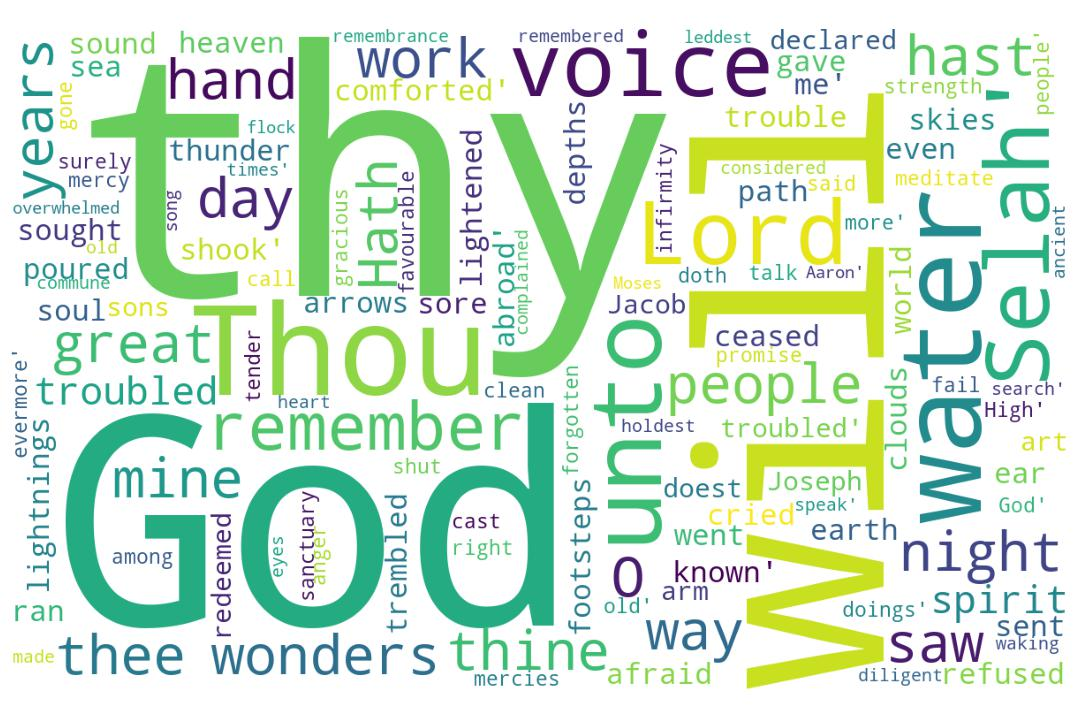
\includegraphics[width=\linewidth]{19OT-Psalms/Psalm77-WordCloud.jpg}
  \caption{Psalm 77 Word Cloud}
  \label{fig:Psalm 77 Word Cloud}
\end{figure}

\marginpar{\scriptsize \centering \fcolorbox{bone}{lime}{\textbf{GOD IS $\hdots$}}\\ (Psalm 77) \begin{compactenum}[I.][8]
    \item \textbf{My Silence} \index[scripture]{Psalms!Psa 077:04}(Psa 77:4)
    \item \textbf{My Searching} \index[scripture]{Psalms!Psa 077:06}(Psa 77:6)
    \item \textbf{My Song} \index[scripture]{Psalms!Psa 077:06}(Psa 77:6)
    \item \textbf{My Spech} \index[scripture]{Psalms!Psa 077:12}(Psa 77:12)
    \item \textbf{My Strength} \index[scripture]{Psalms!Psa 077:14}(Psa 77:14)
    \item \textbf{My Salvation} \index[scripture]{Psalms!Psa 077:15}(Psa 77:15)
    \item \textbf{My Saviour} \index[scripture]{Psalms!Psa 077:20}(Psa 77:20)
\end{compactenum}}
    

\marginpar{\scriptsize \centering \fcolorbox{bone}{yellow}{\textbf{A CHANGE OF}}\\
\fcolorbox{bone}{yellow}{\textbf{HEART AND MIND}}\\ (Psalm 77) 
\begin{compactenum}[I.][8]
    \item \textbf{There is Complaining} \index[scripture]{Psalms!Psa 077:03}(Psa 77:3)
    \item \textbf{There is Considering} \index[scripture]{Psalms!Psa 077:05}(Psa 77:5)
    \item \textbf{There is Communing with your Heart} \index[scripture]{Psalms!Psa 077:06}(Psa 77:6)
    \item \textbf{Thinking God Could Cast off his People} \index[scripture]{Psalms!Psa 077:07}(Psa 77:7)
    \item \textbf{But then Calling to Mind (remembering)} \index[scripture]{Psalms!Psa 077:11}(Psa 77:11)
    \item \textbf{And then God Confounds us} \index[scripture]{Psalms!Psa 077:13}(Psa 77:13) with his greatness, goodness, grace ...
    \item \textbf{That we can barely Contemplate Him} \index[scripture]{Psalms!Psa 077:14}(Psa 77:14)
\end{compactenum}}

\marginpar{\scriptsize \centering \fcolorbox{bone}{black}{\textbf{\textcolor{white}{THE PATH TO}}}\\ \fcolorbox{bone}{black}{\textbf{\textcolor{white}{DELIVERANCE}}}\\(Psalm 77) \begin{compactenum}[I.][8]
    \item \textbf{Revulsion} \index[scripture]{Psalms!Psa 077:02}(Psa 77:2)
    \item \textbf{Refusal} \index[scripture]{Psalms!Psa 077:03}(Psa 77:3)
    \item \textbf{Remembering} \index[scripture]{Psalms!Psa 077:03}\index[scripture]{Psalms!Psa 077:06}\index[scripture]{Psalms!Psa 077:11}\index[scripture]{Psalms!Psa 077:06}(Psa 77:3, 6, 10, 11)
    \item \textbf{Result} \index[scripture]{Psalms!Psa 077:10}(Psa 77:10)
    \item \textbf{Realization} \index[scripture]{Psalms!Psa 077:10}\index[scripture]{Psalms!Psa 077:13}(Psa 77:10, 13)
    \item \textbf{Redemption} \index[scripture]{Psalms!Psa 077:15}(Psa 77:15)
    \item \textbf{Revelation} \index[scripture]{Psalms!Psa 077:18}(Psa 77:18)
    \item \textbf{Rescue} \index[scripture]{Psalms!Psa 077:20}(Psa 77:20)
\end{compactenum}}


% \textcolor[cmyk]{0.99998,1,0,0}{
\footnote{\textcolor[rgb]{0.00,0.25,0.00}{\hyperlink{TOC}{Return to end of Table of Contents.}}}\footnote{\href{https://audiobible.com/bible/psalms_77.html}{\textcolor[cmyk]{0.99998,1,0,0}{Psalm 77 Audio}}}\textcolor[cmyk]{0.99998,1,0,0}{To the chief Musician, to Jeduthun, A Psalm of Asaph.}\\
\\
\textcolor[cmyk]{0.99998,1,0,0}{\fcolorbox{bone}{bone}{I} cried unto God with my voice, \emph{even} unto God with my voice; and he gave ear unto me.}
[2] \textcolor[cmyk]{0.99998,1,0,0}{In the day of my trouble \fcolorbox{bone}{bone}{I} sought the Lord: my sore ran in the night, and ceased not: my soul refused to be comforted.}\footnote{\textbf{Psalm 38:7} - For my loins are filled with a loathsome disease: and there is no soundness in my flesh.}
[3] \textcolor[cmyk]{0.99998,1,0,0}{\fcolorbox{bone}{bone}{I} remembered God, and was troubled: \fcolorbox{bone}{bone}{I} complained, and my spirit was overwhelmed. \fcolorbox{bone}{red}{\textcolor{white}{Selah}}.}
[4] \textcolor[cmyk]{0.99998,1,0,0}{Thou holdest mine eyes waking: \fcolorbox{bone}{bone}{I} am so troubled that \fcolorbox{bone}{bone}{I} cannot speak.}
[5] \textcolor[cmyk]{0.99998,1,0,0}{\fcolorbox{bone}{bone}{I} have considered the days of old, the years of ancient times.}\footnote{\textbf{Isaiah 46:10} - Declaring the end from the beginning, and from ancient times the things that are not yet done, saying, My counsel shall stand, and I will do all my pleasure:}
[6] \textcolor[cmyk]{0.99998,1,0,0}{\fcolorbox{bone}{bone}{I} call to remembrance my song in the night: \fcolorbox{bone}{bone}{I} commune with mine own heart: and my spirit made diligent search.}
[7] \textcolor[cmyk]{0.99998,1,0,0}{Will the Lord cast off for ever? and will he be favourable no more?}
[8] \textcolor[cmyk]{0.99998,1,0,0}{Is his mercy clean gone for ever? doth \emph{his} promise fail for evermore?}\footnote{\textbf{1 Kings 8:56} - Blessed be the LORD, that hath given rest unto his people Israel, according to all that he promised: there hath not failed one word of all his good promise, which he promised by the hand of Moses his servant.}
[9] \textcolor[cmyk]{0.99998,1,0,0}{Hath God forgotten to be gracious? hath he in anger shut up his tender mercies? \fcolorbox{bone}{red}{\textcolor{white}{Selah}}.}
[10] \textcolor[cmyk]{0.99998,1,0,0}{And \fcolorbox{bone}{bone}{I} said, This \emph{is} my infirmity: \emph{but} \emph{I} \emph{will} \emph{remember} the years of the right hand of the most High.}
[11] \textcolor[cmyk]{0.99998,1,0,0}{\fcolorbox{bone}{bone}{I} will remember the works of the LORD: surely \fcolorbox{bone}{bone}{I} will remember thy wonders of old.}
[12] \textcolor[cmyk]{0.99998,1,0,0}{\fcolorbox{bone}{bone}{I} will meditate also of all thy work, and talk of thy doings.}
[13] \textcolor[cmyk]{0.99998,1,0,0}{Thy way, O God, \emph{is} in the sanctuary: who \emph{is} \emph{so} great a God as \emph{our} God?}
[14] \textcolor[cmyk]{0.99998,1,0,0}{Thou \emph{art} the God that doest wonders: thou hast declared thy strength among the people.}
[15] \textcolor[cmyk]{0.99998,1,0,0}{Thou hast with \emph{thine} arm redeemed thy people, the sons of Jacob and Joseph. \fcolorbox{bone}{red}{\textcolor{white}{Selah}}.}
[16] \textcolor[cmyk]{0.99998,1,0,0}{The waters saw thee, O God, the waters saw thee; they were afraid: the depths also were troubled.}\footnote{\textbf{Job 41:32-32} - He maketh the deep to boil like a pot: he maketh the sea like a pot of ointment. [32] He maketh a path to shine after him; one would think the deep to be hoary. }\footnote{\textbf{Psalm 68:22} - The Lord said, I will bring again from Bashan, I will bring my people again from the depths of the sea:}
[17] \textcolor[cmyk]{0.99998,1,0,0}{The clouds poured out water: the skies sent out a sound: thine arrows also went abroad.}\footnote{\textbf{Psalm 18:14} - Yea, he sent out his arrows, and scattered them; and he shot out lightnings, and discomfited them.}\footnote{\textbf{Habakkuk 3:11} - The sun and moon stood still in their habitation: at the light of thine arrows they went, and at the shining of thy glittering spear}
[18] \textcolor[cmyk]{0.99998,1,0,0}{The voice of thy thunder \emph{was} in the heaven: the lightnings lightened the world: the earth trembled and shook.}
[19] \textcolor[cmyk]{0.99998,1,0,0}{Thy way \emph{is} in the sea, and thy path in the great waters, and thy footsteps are not known.}
[20] \textcolor[cmyk]{0.99998,1,0,0}{Thou leddest thy people like a flock by the hand of Moses and Aaron.}

\index[NWIV]{19!Psalms!Psa 77:1}\index[AWIP]{I!Psalms!Psa 77:1}\index[AWIP]{cried!Psalms!Psa 77:1}\index[AWIP]{unto!Psalms!Psa 77:1}\index[AWIP]{unto!Psalms!Psa 77:1 (2)}\index[AWIP]{unto!Psalms!Psa 77:1 (3)}\index[AWIP]{God!Psalms!Psa 77:1}\index[AWIP]{God!Psalms!Psa 77:1 (2)}\index[AWIP]{with!Psalms!Psa 77:1}\index[AWIP]{with!Psalms!Psa 77:1 (2)}\index[AWIP]{my!Psalms!Psa 77:1}\index[AWIP]{my!Psalms!Psa 77:1 (2)}\index[AWIP]{voice!Psalms!Psa 77:1}\index[AWIP]{voice!Psalms!Psa 77:1 (2)}\index[AWIP]{\emph{even}!Psalms!Psa 77:1}\index[AWIP]{and!Psalms!Psa 77:1}\index[AWIP]{he!Psalms!Psa 77:1}\index[AWIP]{gave!Psalms!Psa 77:1}\index[AWIP]{ear!Psalms!Psa 77:1}\index[AWIP]{me!Psalms!Psa 77:1}\index[AWIP]{\emph{even}!Psalms!Psa 77:1}

\index[NWIV]{25!Psalms!Psa 77:2}\index[AWIP]{In!Psalms!Psa 77:2}\index[AWIP]{the!Psalms!Psa 77:2}\index[AWIP]{the!Psalms!Psa 77:2 (2)}\index[AWIP]{the!Psalms!Psa 77:2 (3)}\index[AWIP]{day!Psalms!Psa 77:2}\index[AWIP]{of!Psalms!Psa 77:2}\index[AWIP]{my!Psalms!Psa 77:2}\index[AWIP]{my!Psalms!Psa 77:2 (2)}\index[AWIP]{my!Psalms!Psa 77:2 (3)}\index[AWIP]{trouble!Psalms!Psa 77:2}\index[AWIP]{I!Psalms!Psa 77:2}\index[AWIP]{sought!Psalms!Psa 77:2}\index[AWIP]{Lord!Psalms!Psa 77:2}\index[AWIP]{sore!Psalms!Psa 77:2}\index[AWIP]{ran!Psalms!Psa 77:2}\index[AWIP]{in!Psalms!Psa 77:2}\index[AWIP]{night!Psalms!Psa 77:2}\index[AWIP]{and!Psalms!Psa 77:2}\index[AWIP]{ceased!Psalms!Psa 77:2}\index[AWIP]{not!Psalms!Psa 77:2}\index[AWIP]{soul!Psalms!Psa 77:2}\index[AWIP]{refused!Psalms!Psa 77:2}\index[AWIP]{to!Psalms!Psa 77:2}\index[AWIP]{be!Psalms!Psa 77:2}\index[AWIP]{comforted!Psalms!Psa 77:2}

\index[NWIV]{14!Psalms!Psa 77:3}\index[AWIP]{I!Psalms!Psa 77:3}\index[AWIP]{I!Psalms!Psa 77:3 (2)}\index[AWIP]{remembered!Psalms!Psa 77:3}\index[AWIP]{God!Psalms!Psa 77:3}\index[AWIP]{and!Psalms!Psa 77:3}\index[AWIP]{and!Psalms!Psa 77:3 (2)}\index[AWIP]{was!Psalms!Psa 77:3}\index[AWIP]{was!Psalms!Psa 77:3 (2)}\index[AWIP]{troubled!Psalms!Psa 77:3}\index[AWIP]{complained!Psalms!Psa 77:3}\index[AWIP]{my!Psalms!Psa 77:3}\index[AWIP]{spirit!Psalms!Psa 77:3}\index[AWIP]{overwhelmed!Psalms!Psa 77:3}\index[AWIP]{Selah!Psalms!Psa 77:3}

\index[NWIV]{13!Psalms!Psa 77:4}\index[AWIP]{Thou!Psalms!Psa 77:4}\index[AWIP]{holdest!Psalms!Psa 77:4}\index[AWIP]{mine!Psalms!Psa 77:4}\index[AWIP]{eyes!Psalms!Psa 77:4}\index[AWIP]{waking!Psalms!Psa 77:4}\index[AWIP]{I!Psalms!Psa 77:4}\index[AWIP]{I!Psalms!Psa 77:4 (2)}\index[AWIP]{am!Psalms!Psa 77:4}\index[AWIP]{so!Psalms!Psa 77:4}\index[AWIP]{troubled!Psalms!Psa 77:4}\index[AWIP]{that!Psalms!Psa 77:4}\index[AWIP]{cannot!Psalms!Psa 77:4}\index[AWIP]{speak!Psalms!Psa 77:4}

\index[NWIV]{12!Psalms!Psa 77:5}\index[AWIP]{I!Psalms!Psa 77:5}\index[AWIP]{have!Psalms!Psa 77:5}\index[AWIP]{considered!Psalms!Psa 77:5}\index[AWIP]{the!Psalms!Psa 77:5}\index[AWIP]{the!Psalms!Psa 77:5 (2)}\index[AWIP]{days!Psalms!Psa 77:5}\index[AWIP]{of!Psalms!Psa 77:5}\index[AWIP]{of!Psalms!Psa 77:5 (2)}\index[AWIP]{old!Psalms!Psa 77:5}\index[AWIP]{years!Psalms!Psa 77:5}\index[AWIP]{ancient!Psalms!Psa 77:5}\index[AWIP]{times!Psalms!Psa 77:5}

\index[NWIV]{21!Psalms!Psa 77:6}\index[AWIP]{I!Psalms!Psa 77:6}\index[AWIP]{I!Psalms!Psa 77:6 (2)}\index[AWIP]{call!Psalms!Psa 77:6}\index[AWIP]{to!Psalms!Psa 77:6}\index[AWIP]{remembrance!Psalms!Psa 77:6}\index[AWIP]{my!Psalms!Psa 77:6}\index[AWIP]{my!Psalms!Psa 77:6 (2)}\index[AWIP]{song!Psalms!Psa 77:6}\index[AWIP]{in!Psalms!Psa 77:6}\index[AWIP]{the!Psalms!Psa 77:6}\index[AWIP]{night!Psalms!Psa 77:6}\index[AWIP]{commune!Psalms!Psa 77:6}\index[AWIP]{with!Psalms!Psa 77:6}\index[AWIP]{mine!Psalms!Psa 77:6}\index[AWIP]{own!Psalms!Psa 77:6}\index[AWIP]{heart!Psalms!Psa 77:6}\index[AWIP]{and!Psalms!Psa 77:6}\index[AWIP]{spirit!Psalms!Psa 77:6}\index[AWIP]{made!Psalms!Psa 77:6}\index[AWIP]{diligent!Psalms!Psa 77:6}\index[AWIP]{search!Psalms!Psa 77:6}

\index[NWIV]{14!Psalms!Psa 77:7}\index[AWIP]{Will!Psalms!Psa 77:7}\index[AWIP]{the!Psalms!Psa 77:7}\index[AWIP]{Lord!Psalms!Psa 77:7}\index[AWIP]{cast!Psalms!Psa 77:7}\index[AWIP]{off!Psalms!Psa 77:7}\index[AWIP]{for!Psalms!Psa 77:7}\index[AWIP]{ever?!Psalms!Psa 77:7}\index[AWIP]{and!Psalms!Psa 77:7}\index[AWIP]{will!Psalms!Psa 77:7}\index[AWIP]{he!Psalms!Psa 77:7}\index[AWIP]{be!Psalms!Psa 77:7}\index[AWIP]{favourable!Psalms!Psa 77:7}\index[AWIP]{no!Psalms!Psa 77:7}\index[AWIP]{more?!Psalms!Psa 77:7}

\index[NWIV]{13!Psalms!Psa 77:8}\index[AWIP]{Is!Psalms!Psa 77:8}\index[AWIP]{his!Psalms!Psa 77:8}\index[AWIP]{mercy!Psalms!Psa 77:8}\index[AWIP]{clean!Psalms!Psa 77:8}\index[AWIP]{gone!Psalms!Psa 77:8}\index[AWIP]{for!Psalms!Psa 77:8}\index[AWIP]{for!Psalms!Psa 77:8 (2)}\index[AWIP]{ever?!Psalms!Psa 77:8}\index[AWIP]{doth!Psalms!Psa 77:8}\index[AWIP]{\emph{his}!Psalms!Psa 77:8}\index[AWIP]{promise!Psalms!Psa 77:8}\index[AWIP]{fail!Psalms!Psa 77:8}\index[AWIP]{evermore?!Psalms!Psa 77:8}\index[AWIP]{\emph{his}!Psalms!Psa 77:8}

\index[NWIV]{16!Psalms!Psa 77:9}\index[AWIP]{Hath!Psalms!Psa 77:9}\index[AWIP]{God!Psalms!Psa 77:9}\index[AWIP]{forgotten!Psalms!Psa 77:9}\index[AWIP]{to!Psalms!Psa 77:9}\index[AWIP]{be!Psalms!Psa 77:9}\index[AWIP]{gracious?!Psalms!Psa 77:9}\index[AWIP]{hath!Psalms!Psa 77:9}\index[AWIP]{he!Psalms!Psa 77:9}\index[AWIP]{in!Psalms!Psa 77:9}\index[AWIP]{anger!Psalms!Psa 77:9}\index[AWIP]{shut!Psalms!Psa 77:9}\index[AWIP]{up!Psalms!Psa 77:9}\index[AWIP]{his!Psalms!Psa 77:9}\index[AWIP]{tender!Psalms!Psa 77:9}\index[AWIP]{mercies?!Psalms!Psa 77:9}\index[AWIP]{Selah!Psalms!Psa 77:9}

\index[NWIV]{21!Psalms!Psa 77:10}\index[AWIP]{And!Psalms!Psa 77:10}\index[AWIP]{I!Psalms!Psa 77:10}\index[AWIP]{said!Psalms!Psa 77:10}\index[AWIP]{This!Psalms!Psa 77:10}\index[AWIP]{\emph{is}!Psalms!Psa 77:10}\index[AWIP]{my!Psalms!Psa 77:10}\index[AWIP]{infirmity!Psalms!Psa 77:10}\index[AWIP]{\emph{but}!Psalms!Psa 77:10}\index[AWIP]{\emph{I}!Psalms!Psa 77:10}\index[AWIP]{\emph{will}!Psalms!Psa 77:10}\index[AWIP]{\emph{remember}!Psalms!Psa 77:10}\index[AWIP]{the!Psalms!Psa 77:10}\index[AWIP]{the!Psalms!Psa 77:10 (2)}\index[AWIP]{the!Psalms!Psa 77:10 (3)}\index[AWIP]{years!Psalms!Psa 77:10}\index[AWIP]{of!Psalms!Psa 77:10}\index[AWIP]{of!Psalms!Psa 77:10 (2)}\index[AWIP]{right!Psalms!Psa 77:10}\index[AWIP]{hand!Psalms!Psa 77:10}\index[AWIP]{most!Psalms!Psa 77:10}\index[AWIP]{High!Psalms!Psa 77:10}\index[AWIP]{\emph{is}!Psalms!Psa 77:10}\index[AWIP]{\emph{but}!Psalms!Psa 77:10}\index[AWIP]{\emph{I}!Psalms!Psa 77:10}\index[AWIP]{\emph{will}!Psalms!Psa 77:10}\index[AWIP]{\emph{remember}!Psalms!Psa 77:10}

\index[NWIV]{16!Psalms!Psa 77:11}\index[AWIP]{I!Psalms!Psa 77:11}\index[AWIP]{I!Psalms!Psa 77:11 (2)}\index[AWIP]{will!Psalms!Psa 77:11}\index[AWIP]{will!Psalms!Psa 77:11 (2)}\index[AWIP]{remember!Psalms!Psa 77:11}\index[AWIP]{remember!Psalms!Psa 77:11 (2)}\index[AWIP]{the!Psalms!Psa 77:11}\index[AWIP]{the!Psalms!Psa 77:11 (2)}\index[AWIP]{works!Psalms!Psa 77:11}\index[AWIP]{of!Psalms!Psa 77:11}\index[AWIP]{of!Psalms!Psa 77:11 (2)}\index[AWIP]{LORD!Psalms!Psa 77:11}\index[AWIP]{surely!Psalms!Psa 77:11}\index[AWIP]{thy!Psalms!Psa 77:11}\index[AWIP]{wonders!Psalms!Psa 77:11}\index[AWIP]{old!Psalms!Psa 77:11}

\index[NWIV]{13!Psalms!Psa 77:12}\index[AWIP]{I!Psalms!Psa 77:12}\index[AWIP]{will!Psalms!Psa 77:12}\index[AWIP]{meditate!Psalms!Psa 77:12}\index[AWIP]{also!Psalms!Psa 77:12}\index[AWIP]{of!Psalms!Psa 77:12}\index[AWIP]{of!Psalms!Psa 77:12 (2)}\index[AWIP]{all!Psalms!Psa 77:12}\index[AWIP]{thy!Psalms!Psa 77:12}\index[AWIP]{thy!Psalms!Psa 77:12 (2)}\index[AWIP]{work!Psalms!Psa 77:12}\index[AWIP]{and!Psalms!Psa 77:12}\index[AWIP]{talk!Psalms!Psa 77:12}\index[AWIP]{doings!Psalms!Psa 77:12}

\index[NWIV]{17!Psalms!Psa 77:13}\index[AWIP]{Thy!Psalms!Psa 77:13}\index[AWIP]{way!Psalms!Psa 77:13}\index[AWIP]{O!Psalms!Psa 77:13}\index[AWIP]{God!Psalms!Psa 77:13}\index[AWIP]{God!Psalms!Psa 77:13 (2)}\index[AWIP]{\emph{is}!Psalms!Psa 77:13}\index[AWIP]{\emph{is}!Psalms!Psa 77:13 (2)}\index[AWIP]{in!Psalms!Psa 77:13}\index[AWIP]{the!Psalms!Psa 77:13}\index[AWIP]{sanctuary!Psalms!Psa 77:13}\index[AWIP]{who!Psalms!Psa 77:13}\index[AWIP]{\emph{so}!Psalms!Psa 77:13}\index[AWIP]{great!Psalms!Psa 77:13}\index[AWIP]{a!Psalms!Psa 77:13}\index[AWIP]{as!Psalms!Psa 77:13}\index[AWIP]{\emph{our}!Psalms!Psa 77:13}\index[AWIP]{God?!Psalms!Psa 77:13}\index[AWIP]{\emph{is}!Psalms!Psa 77:13}\index[AWIP]{\emph{is}!Psalms!Psa 77:13 (2)}\index[AWIP]{\emph{so}!Psalms!Psa 77:13}\index[AWIP]{\emph{our}!Psalms!Psa 77:13}

\index[NWIV]{15!Psalms!Psa 77:14}\index[AWIP]{Thou!Psalms!Psa 77:14}\index[AWIP]{\emph{art}!Psalms!Psa 77:14}\index[AWIP]{the!Psalms!Psa 77:14}\index[AWIP]{the!Psalms!Psa 77:14 (2)}\index[AWIP]{God!Psalms!Psa 77:14}\index[AWIP]{that!Psalms!Psa 77:14}\index[AWIP]{doest!Psalms!Psa 77:14}\index[AWIP]{wonders!Psalms!Psa 77:14}\index[AWIP]{thou!Psalms!Psa 77:14}\index[AWIP]{hast!Psalms!Psa 77:14}\index[AWIP]{declared!Psalms!Psa 77:14}\index[AWIP]{thy!Psalms!Psa 77:14}\index[AWIP]{strength!Psalms!Psa 77:14}\index[AWIP]{among!Psalms!Psa 77:14}\index[AWIP]{people!Psalms!Psa 77:14}\index[AWIP]{\emph{art}!Psalms!Psa 77:14}

\index[NWIV]{15!Psalms!Psa 77:15}\index[AWIP]{Thou!Psalms!Psa 77:15}\index[AWIP]{hast!Psalms!Psa 77:15}\index[AWIP]{with!Psalms!Psa 77:15}\index[AWIP]{\emph{thine}!Psalms!Psa 77:15}\index[AWIP]{arm!Psalms!Psa 77:15}\index[AWIP]{redeemed!Psalms!Psa 77:15}\index[AWIP]{thy!Psalms!Psa 77:15}\index[AWIP]{people!Psalms!Psa 77:15}\index[AWIP]{the!Psalms!Psa 77:15}\index[AWIP]{sons!Psalms!Psa 77:15}\index[AWIP]{of!Psalms!Psa 77:15}\index[AWIP]{Jacob!Psalms!Psa 77:15}\index[AWIP]{and!Psalms!Psa 77:15}\index[AWIP]{Joseph!Psalms!Psa 77:15}\index[AWIP]{Selah!Psalms!Psa 77:15}\index[AWIP]{\emph{thine}!Psalms!Psa 77:15}

\index[NWIV]{18!Psalms!Psa 77:16}\index[AWIP]{The!Psalms!Psa 77:16}\index[AWIP]{waters!Psalms!Psa 77:16}\index[AWIP]{waters!Psalms!Psa 77:16 (2)}\index[AWIP]{saw!Psalms!Psa 77:16}\index[AWIP]{saw!Psalms!Psa 77:16 (2)}\index[AWIP]{thee!Psalms!Psa 77:16}\index[AWIP]{thee!Psalms!Psa 77:16 (2)}\index[AWIP]{O!Psalms!Psa 77:16}\index[AWIP]{God!Psalms!Psa 77:16}\index[AWIP]{the!Psalms!Psa 77:16}\index[AWIP]{the!Psalms!Psa 77:16 (2)}\index[AWIP]{they!Psalms!Psa 77:16}\index[AWIP]{were!Psalms!Psa 77:16}\index[AWIP]{were!Psalms!Psa 77:16 (2)}\index[AWIP]{afraid!Psalms!Psa 77:16}\index[AWIP]{depths!Psalms!Psa 77:16}\index[AWIP]{also!Psalms!Psa 77:16}\index[AWIP]{troubled!Psalms!Psa 77:16}

\index[NWIV]{16!Psalms!Psa 77:17}\index[AWIP]{The!Psalms!Psa 77:17}\index[AWIP]{clouds!Psalms!Psa 77:17}\index[AWIP]{poured!Psalms!Psa 77:17}\index[AWIP]{out!Psalms!Psa 77:17}\index[AWIP]{out!Psalms!Psa 77:17 (2)}\index[AWIP]{water!Psalms!Psa 77:17}\index[AWIP]{the!Psalms!Psa 77:17}\index[AWIP]{skies!Psalms!Psa 77:17}\index[AWIP]{sent!Psalms!Psa 77:17}\index[AWIP]{a!Psalms!Psa 77:17}\index[AWIP]{sound!Psalms!Psa 77:17}\index[AWIP]{thine!Psalms!Psa 77:17}\index[AWIP]{arrows!Psalms!Psa 77:17}\index[AWIP]{also!Psalms!Psa 77:17}\index[AWIP]{went!Psalms!Psa 77:17}\index[AWIP]{abroad!Psalms!Psa 77:17}

\index[NWIV]{19!Psalms!Psa 77:18}\index[AWIP]{The!Psalms!Psa 77:18}\index[AWIP]{voice!Psalms!Psa 77:18}\index[AWIP]{of!Psalms!Psa 77:18}\index[AWIP]{thy!Psalms!Psa 77:18}\index[AWIP]{thunder!Psalms!Psa 77:18}\index[AWIP]{\emph{was}!Psalms!Psa 77:18}\index[AWIP]{in!Psalms!Psa 77:18}\index[AWIP]{the!Psalms!Psa 77:18}\index[AWIP]{the!Psalms!Psa 77:18 (2)}\index[AWIP]{the!Psalms!Psa 77:18 (3)}\index[AWIP]{the!Psalms!Psa 77:18 (4)}\index[AWIP]{heaven!Psalms!Psa 77:18}\index[AWIP]{lightnings!Psalms!Psa 77:18}\index[AWIP]{lightened!Psalms!Psa 77:18}\index[AWIP]{world!Psalms!Psa 77:18}\index[AWIP]{earth!Psalms!Psa 77:18}\index[AWIP]{trembled!Psalms!Psa 77:18}\index[AWIP]{and!Psalms!Psa 77:18}\index[AWIP]{shook!Psalms!Psa 77:18}\index[AWIP]{\emph{was}!Psalms!Psa 77:18}

\index[NWIV]{19!Psalms!Psa 77:19}\index[AWIP]{Thy!Psalms!Psa 77:19}\index[AWIP]{way!Psalms!Psa 77:19}\index[AWIP]{\emph{is}!Psalms!Psa 77:19}\index[AWIP]{in!Psalms!Psa 77:19}\index[AWIP]{in!Psalms!Psa 77:19 (2)}\index[AWIP]{the!Psalms!Psa 77:19}\index[AWIP]{the!Psalms!Psa 77:19 (2)}\index[AWIP]{sea!Psalms!Psa 77:19}\index[AWIP]{and!Psalms!Psa 77:19}\index[AWIP]{and!Psalms!Psa 77:19 (2)}\index[AWIP]{thy!Psalms!Psa 77:19}\index[AWIP]{thy!Psalms!Psa 77:19 (2)}\index[AWIP]{path!Psalms!Psa 77:19}\index[AWIP]{great!Psalms!Psa 77:19}\index[AWIP]{waters!Psalms!Psa 77:19}\index[AWIP]{footsteps!Psalms!Psa 77:19}\index[AWIP]{are!Psalms!Psa 77:19}\index[AWIP]{not!Psalms!Psa 77:19}\index[AWIP]{known!Psalms!Psa 77:19}\index[AWIP]{\emph{is}!Psalms!Psa 77:19}

\index[NWIV]{14!Psalms!Psa 77:20}\index[AWIP]{Thou!Psalms!Psa 77:20}\index[AWIP]{leddest!Psalms!Psa 77:20}\index[AWIP]{thy!Psalms!Psa 77:20}\index[AWIP]{people!Psalms!Psa 77:20}\index[AWIP]{like!Psalms!Psa 77:20}\index[AWIP]{a!Psalms!Psa 77:20}\index[AWIP]{flock!Psalms!Psa 77:20}\index[AWIP]{by!Psalms!Psa 77:20}\index[AWIP]{the!Psalms!Psa 77:20}\index[AWIP]{hand!Psalms!Psa 77:20}\index[AWIP]{of!Psalms!Psa 77:20}\index[AWIP]{Moses!Psalms!Psa 77:20}\index[AWIP]{and!Psalms!Psa 77:20}\index[AWIP]{Aaron!Psalms!Psa 77:20}


\section{Psalm 77 Outlines}

\subsection{My Outlines} 

\subsubsection{God Is ... }
\index[speaker]{Keith Anthony!Psalm 077 (God Is ...)}
\index[series]{Psalms (Keith Anthony)!Psalm 077 (God Is ...)}
\index[date]{2015/08/21!Psalm 077 (God Is ...) (Keith Anthony)}
\begin{compactenum}[I.]
    \item \textbf{My Silence} \index[scripture]{Psalms!Psa 077:04}(Psa 77:4)
    \item \textbf{My Searching} \index[scripture]{Psalms!Psa 077:06}(Psa 77:6)
    \item \textbf{My Song} \index[scripture]{Psalms!Psa 077:06}(Psa 77:6)
    \item \textbf{My Spech} \index[scripture]{Psalms!Psa 077:12}(Psa 77:12)
    \item \textbf{My Strength} \index[scripture]{Psalms!Psa 077:14}(Psa 77:14)
    \item \textbf{My Salvation} \index[scripture]{Psalms!Psa 077:15}(Psa 77:15)
    \item \textbf{My Saviour} \index[scripture]{Psalms!Psa 077:20}(Psa 77:20)
\end{compactenum}

\subsubsection{A Change of Heart and Mind}
\index[speaker]{Keith Anthony!Psalm 077 (A Change of Heart and Mind }
\index[series]{Psalms (Keith Anthony)!Psalm 077 (A Change of Heart and Mind}
\index[date]{2015/08/21!Psalm 077 (A Change of Heart and Mind) (Keith Anthony)}
\begin{compactenum}[I.]
    \item \textbf{There is Complaining} \index[scripture]{Psalms!Psa 077:03}(Psa 77:3)
    \item \textbf{There is Considering} \index[scripture]{Psalms!Psa 077:05}(Psa 77:5)
    \item \textbf{There is Communing with your Heart} \index[scripture]{Psalms!Psa 077:06}(Psa 77:6)
    \item \textbf{Thinking God Could Cast off his People} \index[scripture]{Psalms!Psa 077:07}(Psa 77:7)
    \item \textbf{But then Calling to Mind (remembering)} \index[scripture]{Psalms!Psa 077:11}(Psa 77:11)
    \item \textbf{And then God Confounds us} \index[scripture]{Psalms!Psa 077:13}(Psa 77:13) with his greatness, goodness, grace ...
    \item \textbf{That we can barely Contemplate Him} \index[scripture]{Psalms!Psa 077:14}(Psa 77:14)
\end{compactenum}

\subsubsection{Israel's Path to Deliverance}
\index[speaker]{Keith Anthony!Psalm 077 (Israel's Path to Deliverance}
\index[series]{Psalms (Keith Anthony)!Psalm 077 (Israel's Path to Deliverance}
\index[date]{2021/09/05!Psalm 077 (Israel's Path to Deliverance) (Keith Anthony)}
\begin{compactenum}[I.][8]
    \item \textbf{Revulsion} \index[scripture]{Psalms!Psa 077:02}(Psa 77:2)
    \item \textbf{Refusal} \index[scripture]{Psalms!Psa 077:03}(Psa 77:3)
    \item \textbf{Remembering} \index[scripture]{Psalms!Psa 077:03}\index[scripture]{Psalms!Psa 077:06}\index[scripture]{Psalms!Psa 077:11}\index[scripture]{Psalms!Psa 077:06}(Psa 77:3, 6, 10, 11)
    \item \textbf{Realization} \index[scripture]{Psalms!Psa 077:10}\index[scripture]{Psalms!Psa 077:13}(Psa 77:10, 13)
    \item \textbf{Redemption} \index[scripture]{Psalms!Psa 077:15}(Psa 77:15)
    \item \textbf{Revelation} \index[scripture]{Psalms!Psa 077:18}(Psa 77:18)
    \item \textbf{Rescue} \index[scripture]{Psalms!Psa 077:20}(Psa 77:20)
\end{compactenum}


\section{Outlines from Others}

%\subsubsection{What to do when you start talking to yourself}
%\index[speaker]{Richard Drummond!Psalm 077 (What to do when you start talking to yourself}
%\index[series]{Psalms (Richard Drummond)!Psalm 077 (What to do when you start talking to yourself)}
%\index[date]{2014/05/25!Psalm 077 (What to do when you start talking to yourself)) (Richard Drummond)}
%\begin{compactenum}[I.][4]
%	\item Stop and \textbf{Remember} the years at the years of the right hand of God ... forget the past ...cannot change history \index[scripture]{Psalms!Psa 077:10}(Psalm 77:10)
%	\item \textbf{Remember} the works of the Lord \index[scripture]{Mathew!Matt 06:25--28}(Mathew 6:25--28) $\hdots$ \index[scripture]{Psalms!Psa 077:11}(Psalm 77:11)
%	\item \textbf{Remember} the wonders of old ...   \index[scripture]{Psalms!Psa 077:11}(Psalm 77:11)
%	\item \textbf{Meditate} on God's  work ... \index[scripture]{Joshua!Josh 01:08}Joshua 1:8, only mention of the word "success" ...  \index[scripture]{Psalms!Psa 001:02}Psalm 1:2,  \index[scripture]{Psalms!Psa 063:06}Psalm 63:6,  \index[scripture]{Psalms!Psa 143:05}Psalm 143:5,  \index[scripture]{Psalms!Psa 077:12}(Psalm 77:12)
%\end{compactenum}

\section{Psalm 77 Comments}

\subsection{Numeric Nuggets}
Verses 4, 8, and 12 have 13 words. Verses 1 and 16 have 13 unique words. The word ``I'' is used 13 times in the chapter (the word ``I'' in italics is found once). The 13$^{th}$ word in the chapter is the word ``voice'' (it is also the 7$^{th}$ word). The use of the word ``I'' ceases in verse 12. Verse 13 seems to be a transition verse: it has 13 words that are not italic! Verse 13 contains the word \emph{our} indicating the psalmist's recognition and acceptance of his place among God's redeemed people, Israel. The psalmist sends out six questions in verses 7-9, before the second ``Selah'' in verse 9 (the other two are in verses 3 and 15). Three ``Selahs'' are likely quite significant and likely have something to do with specific dealings of the LORD with Tribulation Israel.

\subsection{Psalm 77 Introduction}
The doctrinal content of this psalm is the Second Advent of Jesus Christ and his rescue of his people Israel. Spiritually, a sinner must recognize his desperate, deplorable, and hopeless condition before he will cry out to God for salvation. 

\subsection{Psalm 77:1}
Jeremiah 51:16 connects the ``voice'' with lightnings (as seen in verse 18).\footnote{\textbf{Jeremiah 51:16} - When he uttereth his voice, there is a multitude of waters in the heavens; and he causeth the vapours to ascend from the ends of the earth: he maketh lightnings with rain, and bringeth forth the wind out of his treasures.}

\subsection{Psalm 77:6}
Compare this ``diligent search'' with the diligent search carried out by the wicked.\footnote{\textbf{Psalm 64:6} - They search out iniquities; they accomplish a diligent search: both the inward thought of every one of them, and the heart, is deep. }

\subsection{Psalm 77:7-9}
The psalmist poses six questions:
\begin{compactenum}
    \item Will the Lord cast off for ever?
    \item Will he be favourable no more?
    \item Is his mercy clean gone for ever?
    \item Doth his promise fail for evermore?
    \item Hath God forgotten to be gracious 
    \item Hath he in anger shut up his tender mercies?\\
\end{compactenum}

\subsection{Psalm 77:10}
Note the mention of body, soul, and spirit in verses 2 and 3.
\begin{center}

\begin{table}[ht]
\centering
\begin{tabular}{|p{.5in}|p{3.5in}|}
\hline

\textcolor[rgb]{0.00,0.00,1.00}{AV} & \textcolor[rgb]{0.00,0.00,1.00}{And I said, This \emph{is} my infirmity: \emph{but} \emph{I} \emph{will} \emph{remember} the years of the right hand of the most High.} \\ \hline 

\hline
\hline


ASV &  And I said, This is my infirmity; But I will remember the years of the right hand of the Most High. \\ \hline
%
CEB &  It’s my misfortune, I thought,  that the strong hand of the Most High is different now.\\ \hline
%
ESV & Then I said, ``I will appeal to this, to the years of the right hand of the Most High.'' \\ \hline
%
NASV &  Then I said, “It is my grief, That the right hand of the Most High has changed.” \\ \hline
%
MEV & Then I said, “This is my grief;  yet I will remember the years of the right hand of the Most High.” \\ \hline
%
NIV &  Then I thought, “To this I will appeal:  the years when the Most High stretched out his right hand. \\ \hline
%
NKJV &  And I said, “This is my anguish;
But I will remember the years of the right hand of the Most High.”\\ \hline
%
RSV &  And I say, “It is my grief that the right hand of the Most High has changed.”. \\ \hline

\hline
\hline

\multicolumn{2}{|p{4.3in}|}{{\textcolor{jungle}{The word ``infirmity'' is changed to “anguish,” “grief,” and “misfortune.” It is removed completely in the ESV and NIV. The effect is destroying the connection to “sore” in verse 2. The psalmist here, who typifies the Tribulation Jew, has 2 infirmities: A physical one, and a spiritual one. The infirmity, or infirmities, are emphasized by the word ``my.'' Ruckman points out that and infirmity is a weakness as in 2 Corinthians 11:30 and 12:5.\cite{Ruckman1992PsalmsV2}.}}} \\ \hline

\end{tabular}
\caption[Corruption Alert: Psalm 77:10]{Corruption Alert: Psalm 77:10} \label{table:Corruption Psalm 77:10}

\end{table}

\end{center}




\noindent The answer (to the six questions), in general, with respect to Israel, is a resounding ``No!'' The mercies are called for by David in 2 Samuel 24:14 and 1 Chronicles 21:13.\footnote{\textbf{2 Samuel 24:14} - And David said unto Gad, I am in a great strait: let us fall now into the hand of the LORD; for his mercies are great: and let me not fall into the hand of man.}\footnote{\textbf{1 Chronicles 21:13} - And David said unto Gad, I am in a great strait: let me fall now into the hand of the LORD; for very great are his mercies: but let me not fall into the hand of man.}\cite{Ruckman1992PsalmsV2}

\subsection{Psalm 77:9}
The phrase ``tender mercies'' shows up eleven times in scripture, ten occurrences of which speak of the Lord's ``tender mercies.'' All of these are in Psalms (Psalms 25:6, 40:11, 51:1, 69:16, 77:9, 79:8, 103:4, 119:77, 119:156, and  145:9.) Number eleven describes the ``tender mercies'' of the wicked, called cruel. So, question number six is answered (confirmed in Lamentations 3:22). \footnote{\textbf{Lamentations 3:22} - It is of the LORD’S mercies that we are not consumed, because his compassions fail not.} But, in Jeremiah 16:5, they are temporarily taken away.\footnote{\textbf{Jeremiah 16:5} - For thus saith the LORD, Enter not into the house of mourning, neither go to lament nor bemoan them: for I have taken away my peace from this people, saith the LORD, even lovingkindness and mercies.}\cite{Ruckman1992PsalmsV2}

\subsection{Psalm 77:17-19}
Psalm 18 is a wonderful parallel passage to Psalm 77. Verse 14 speaks of God's arrows and lightnings. It also speaks of the ``channels'' of waters spoke of here in verse 18. This ``path in the great waters'' is the route the LORD will take with his armies for is return at the Second Advent.\footnote{\textbf{PSalm 18} - I will love thee, O LORD, my strength. [2] The LORD is my rock, and my fortress, and my deliverer; my God, my strength, in whom I will trust; my buckler, and the horn of my salvation, and my high tower. [3] I will call upon the LORD, who is worthy to be praised: so shall I be saved from mine enemies. [4] The sorrows of death compassed me, and the floods of ungodly men made me afraid. [5] The sorrows of hell compassed me about: the snares of death prevented me. [6] In my distress I called upon the LORD, and cried unto my God: he heard my voice out of his temple, and my cry came before him, even into his ears. [7] Then the earth shook and trembled; the foundations also of the hills moved and were shaken, because he was wroth. [8] There went up a smoke out of his nostrils, and fire out of his mouth devoured: coals were kindled by it. [9] He bowed the heavens also, and came down: and darkness was under his feet. [10] And he rode upon a cherub, and did fly: yea, he did fly upon the wings of the wind. [11] He made darkness his secret place; his pavilion round about him were dark waters and thick clouds of the skies. [12] At the brightness that was before him his thick clouds passed, hail stones and coals of fire. [13] The LORD also thundered in the heavens, and the Highest gave his voice; hail stones and coals of fire. [14] Yea, he sent out his arrows, and scattered them; and he shot out lightnings, and discomfited them. [15] Then the channels of waters were seen, and the foundations of the world were discovered at thy rebuke, O LORD, at the blast of the breath of thy nostrils. [16] He sent from above, he took me, he drew me out of many waters. [17] He delivered me from my strong enemy, and from them which hated me: for they were too strong for me. [18] They prevented me in the day of my calamity: but the LORD was my stay. [19] He brought me forth also into a large place; he delivered me, because he delighted in me. [20] The LORD rewarded me according to my righteousness; according to the cleanness of my hands hath he recompensed me. [21] For I have kept the ways of the LORD, and have not wickedly departed from my God. [22] For all his judgments were before me, and I did not put away his statutes from me. [23] I was also upright before him, and I kept myself from mine iniquity. [24] Therefore hath the LORD recompensed me according to my righteousness, according to the cleanness of my hands in his eyesight. [25] With the merciful thou wilt shew thyself merciful; with an upright man thou wilt shew thyself upright; [26] With the pure thou wilt shew thyself pure; and with the froward thou wilt shew thyself froward. [27] For thou wilt save the afflicted people; but wilt bring down high looks. [28] For thou wilt light my candle: the LORD my God will enlighten my darkness. [29] For by thee I have run through a troop; and by my God have I leaped over a wall. [30] As for God, his way is perfect: the word of the LORD is tried: he is a buckler to all those that trust in him. [31] For who is God save the LORD? or who is a rock save our God? [32] It is God that girdeth me with strength, and maketh my way perfect. [33] He maketh my feet like hinds’ feet, and setteth me upon my high places. [34] He teacheth my hands to war, so that a bow of steel is broken by mine arms. [35] Thou hast also given me the shield of thy salvation: and thy right hand hath holden me up, and thy gentleness hath made me great. [36] Thou hast enlarged my steps under me, that my feet did not slip. [37] I have pursued mine enemies, and overtaken them: neither did I turn again till they were consumed. [38] I have wounded them that they were not able to rise: they are fallen under my feet. [39] For thou hast girded me with strength unto the battle: thou hast subdued under me those that rose up against me. [40] Thou hast also given me the necks of mine enemies; that I might destroy them that hate me. [41] They cried, but there was none to save them: even unto the LORD, but he answered them not. [42] Then did I beat them small as the dust before the wind: I did cast them out as the dirt in the streets. [43] Thou hast delivered me from the strivings of the people; and thou hast made me the head of the heathen: a people whom I have not known shall serve me. [44] As soon as they hear of me, they shall obey me: the strangers shall submit themselves unto me. [45] The strangers shall fade away, and be afraid out of their close places. [46] The LORD liveth; and blessed be my rock; and let the God of my salvation be exalted. [47] It is God that avengeth me, and subdueth the people under me. [48] He delivereth me from mine enemies: yea, thou liftest me up above those that rise up against me: thou hast delivered me from the violent man. [49] Therefore will I give thanks unto thee, O LORD, among the heathen, and sing praises unto thy name. [50] Great deliverance giveth he to his king; and sheweth mercy to his anointed, to David, and to his seed for evermore.}\cite{Ruckman1992PsalmsV2}

\subsection{Psalm 77:20}
Another comparison is the in Numbers 33:1.\footnote{\textbf{Numbers 33:1} - These are the journeys of the children of Israel, which went forth out of the land of Egypt with their armies under the hand of Moses and Aaron.}\cite{Ruckman1992PsalmsV2}


\subsection{Psalm77 Repeated Phrases}


%%%%%%%%%%
%%%%%%%%%%
\normalsize
 
\begin{center}
\begin{longtable}{|p{3.0in}|p{0.5in}|}
\caption[Psalm77 Repeated Phrases]{Psalm77 Repeated Phrases}\label{table:Repeated Phrases Psalm77} \\
\hline \multicolumn{1}{|c|}{\textbf{Phrase}} & \multicolumn{1}{c|}{\textbf{Frequency}} \\ \hline 
\endfirsthead
 
\multicolumn{2}{c}
{{\bfseries \tablename\ \thetable{} -- continued from previous page}} \\  
\hline \multicolumn{1}{|c|}{\textbf{Phrase}} & \multicolumn{1}{c|}{\textbf{Frequency}} \\ \hline 
\endhead
 
\hline \multicolumn{2}{c}{{ }} \\ \hline
\endfoot 
in the & 6\\ \hline 
of the & 3\\ \hline 
I will & 3\\ \hline 
\end{longtable}
\end{center}



%%%%%%%%%%
%%%%%%%%%%



\section{Psalm 77 Word Statistics}


%%%%%%%%%%
%%%%%%%%%%
\normalsize
 
\begin{center}
\begin{longtable}{l|c|c|c|c}
\caption[Psalm 77 Statistics]{Psalm 77 Statistics}\label{table:Statistics for Psalm 77} \\
\hline \multicolumn{1}{|c|}{\textbf{Verse(s)}} & \multicolumn{1}{|c|}{\textbf{Count}} & \multicolumn{1}{|c|}{\textbf{Unique}} & \multicolumn{1}{|c|}{\textbf{Italics}} & \multicolumn{1}{|c|}{\textbf{Uniq Italic}}  \\ \hline 
\endfirsthead
 
\multicolumn{5}{c}
{{\bfseries \tablename\ \thetable{} -- continued from previous page}} \\  
\hline \multicolumn{1}{|c|}{\textbf{Verse(s)}} & \multicolumn{1}{|c|}{\textbf{Count}} & \multicolumn{1}{|c|}{\textbf{Unique}} & \multicolumn{1}{|c|}{\textbf{Italics}} & \multicolumn{1}{|c|}{\textbf{Uniq Italic}}  \\ \hline 
\endhead
 
\hline \multicolumn{5}{|r|}{{Continued if needed}} \\ \hline
\endfoot 
1 & 19 & 13 & 1 & 1\\ \hline
2 & 25 & 21 & 0 & 0\\ \hline
3 & 14 & 11 & 0 & 0\\ \hline
4 & 13 & 12 & 0 & 0\\ \hline
5 & 12 & 10 & 0 & 0\\ \hline
6 & 21 & 19 & 0 & 0\\ \hline
7 & 14 & 14 & 0 & 0\\ \hline
8 & 13 & 12 & 1 & 1\\ \hline
9 & 16 & 16 & 0 & 0\\ \hline
10 & 21 & 18 & 5 & 5\\ \hline
11 & 16 & 11 & 0 & 0\\ \hline
12 & 13 & 11 & 0 & 0\\ \hline
13 & 17 & 14 & 4 & 3\\ \hline
14 & 15 & 14 & 1 & 1\\ \hline
15 & 15 & 15 & 1 & 1\\ \hline
16 & 18 & 13 & 0 & 0\\ \hline
17 & 16 & 15 & 0 & 0\\ \hline
18 & 19 & 16 & 1 & 1\\ \hline
19 & 19 & 15 & 1 & 1\\ \hline
20 & 14 & 14 & 0 & 0\\ \hline
Total & 330 & 180 & 15 & 12
\end{longtable}
\end{center}



%%%%%%%%%%
%%%%%%%%%%


\subsection{Psalm 77 Words by Frequency}


%%%%%%%%%%
%%%%%%%%%%
\normalsize
 
\begin{center}
\begin{longtable}{l|r}
\caption[Psalm 77 Words by Frequency]{Psalm 77 Words by Frequency}\label{table:WordsbyFrequency for Psalm 77} \\
\hline \multicolumn{1}{|c|}{\textbf{Word}} & \multicolumn{1}{c|}{\textbf{Frequency}} \\ \hline 
\endfirsthead
 
\multicolumn{2}{c}
{{\bfseries \tablename\ \thetable{} -- continued from previous page}} \\  
\hline \multicolumn{1}{|c|}{\textbf{Word}} & \multicolumn{1}{c|}{\textbf{Frequency}} \\ \hline 
\endhead
 
\hline \multicolumn{2}{c}{{ }} \\ \hline
\endfoot 
the & 26\\ \hline 
I & 13\\ \hline 
and & 12\\ \hline 
of & 12\\ \hline 
God & 9\\ \hline 
my & 9\\ \hline 
thy & 9\\ \hline 
in & 7\\ \hline 
with & 4\\ \hline 
Thou & 4\\ \hline 
will & 4\\ \hline 
\emph{is} & 4\\ \hline 
unto & 3\\ \hline 
voice & 3\\ \hline 
he & 3\\ \hline 
to & 3\\ \hline 
be & 3\\ \hline 
troubled & 3\\ \hline 
Selah & 3\\ \hline 
for & 3\\ \hline 
also & 3\\ \hline 
a & 3\\ \hline 
people & 3\\ \hline 
The & 3\\ \hline 
waters & 3\\ \hline 
Lord & 2\\ \hline 
night & 2\\ \hline 
not & 2\\ \hline 
was & 2\\ \hline 
spirit & 2\\ \hline 
mine & 2\\ \hline 
that & 2\\ \hline 
old & 2\\ \hline 
years & 2\\ \hline 
ever & 2\\ \hline 
his & 2\\ \hline 
hand & 2\\ \hline 
remember & 2\\ \hline 
wonders & 2\\ \hline 
Thy & 2\\ \hline 
way & 2\\ \hline 
O & 2\\ \hline 
great & 2\\ \hline 
hast & 2\\ \hline 
saw & 2\\ \hline 
thee & 2\\ \hline 
were & 2\\ \hline 
out & 2\\ \hline 
cried & 1\\ \hline 
\emph{even} & 1\\ \hline 
gave & 1\\ \hline 
ear & 1\\ \hline 
me & 1\\ \hline 
In & 1\\ \hline 
day & 1\\ \hline 
trouble & 1\\ \hline 
sought & 1\\ \hline 
sore & 1\\ \hline 
ran & 1\\ \hline 
ceased & 1\\ \hline 
soul & 1\\ \hline 
refused & 1\\ \hline 
comforted & 1\\ \hline 
remembered & 1\\ \hline 
complained & 1\\ \hline 
overwhelmed & 1\\ \hline 
holdest & 1\\ \hline 
eyes & 1\\ \hline 
waking & 1\\ \hline 
am & 1\\ \hline 
so & 1\\ \hline 
cannot & 1\\ \hline 
speak & 1\\ \hline 
have & 1\\ \hline 
considered & 1\\ \hline 
days & 1\\ \hline 
ancient & 1\\ \hline 
times & 1\\ \hline 
call & 1\\ \hline 
remembrance & 1\\ \hline 
song & 1\\ \hline 
commune & 1\\ \hline 
own & 1\\ \hline 
heart & 1\\ \hline 
made & 1\\ \hline 
diligent & 1\\ \hline 
search & 1\\ \hline 
Will & 1\\ \hline 
cast & 1\\ \hline 
off & 1\\ \hline 
favourable & 1\\ \hline 
no & 1\\ \hline 
more & 1\\ \hline 
Is & 1\\ \hline 
mercy & 1\\ \hline 
clean & 1\\ \hline 
gone & 1\\ \hline 
doth & 1\\ \hline 
\emph{his} & 1\\ \hline 
promise & 1\\ \hline 
fail & 1\\ \hline 
evermore & 1\\ \hline 
Hath & 1\\ \hline 
forgotten & 1\\ \hline 
gracious & 1\\ \hline 
hath & 1\\ \hline 
anger & 1\\ \hline 
shut & 1\\ \hline 
up & 1\\ \hline 
tender & 1\\ \hline 
mercies & 1\\ \hline 
And & 1\\ \hline 
said & 1\\ \hline 
This & 1\\ \hline 
infirmity & 1\\ \hline 
\emph{but} & 1\\ \hline 
\emph{I} & 1\\ \hline 
\emph{will} & 1\\ \hline 
\emph{remember} & 1\\ \hline 
right & 1\\ \hline 
most & 1\\ \hline 
High & 1\\ \hline 
works & 1\\ \hline 
LORD & 1\\ \hline 
surely & 1\\ \hline 
meditate & 1\\ \hline 
all & 1\\ \hline 
work & 1\\ \hline 
talk & 1\\ \hline 
doings & 1\\ \hline 
sanctuary & 1\\ \hline 
who & 1\\ \hline 
\emph{so} & 1\\ \hline 
as & 1\\ \hline 
\emph{our} & 1\\ \hline 
\emph{art} & 1\\ \hline 
doest & 1\\ \hline 
thou & 1\\ \hline 
declared & 1\\ \hline 
strength & 1\\ \hline 
among & 1\\ \hline 
\emph{thine} & 1\\ \hline 
arm & 1\\ \hline 
redeemed & 1\\ \hline 
sons & 1\\ \hline 
Jacob & 1\\ \hline 
Joseph & 1\\ \hline 
they & 1\\ \hline 
afraid & 1\\ \hline 
depths & 1\\ \hline 
clouds & 1\\ \hline 
poured & 1\\ \hline 
water & 1\\ \hline 
skies & 1\\ \hline 
sent & 1\\ \hline 
sound & 1\\ \hline 
thine & 1\\ \hline 
arrows & 1\\ \hline 
went & 1\\ \hline 
abroad & 1\\ \hline 
thunder & 1\\ \hline 
\emph{was} & 1\\ \hline 
heaven & 1\\ \hline 
lightnings & 1\\ \hline 
lightened & 1\\ \hline 
world & 1\\ \hline 
earth & 1\\ \hline 
trembled & 1\\ \hline 
shook & 1\\ \hline 
sea & 1\\ \hline 
path & 1\\ \hline 
footsteps & 1\\ \hline 
are & 1\\ \hline 
known & 1\\ \hline 
leddest & 1\\ \hline 
like & 1\\ \hline 
flock & 1\\ \hline 
by & 1\\ \hline 
Moses & 1\\ \hline 
Aaron & 1\\ \hline 
\end{longtable}
\end{center}



%%%%%%%%%%
%%%%%%%%%%


\subsection{Psalm 77 Words Alphabetically}


%%%%%%%%%%
%%%%%%%%%%
\normalsize
 
\begin{center}
\begin{longtable}{l|r}
\caption[Psalm 77 Words Alphabetically]{Psalm 77 Words Alphabetically}\label{table:WordsAlphabetically for Psalm 77} \\
\hline \multicolumn{1}{|c|}{\textbf{Word}} & \multicolumn{1}{c|}{\textbf{Frequency}} \\ \hline 
\endfirsthead
 
\multicolumn{2}{c}
{{\bfseries \tablename\ \thetable{} -- continued from previous page}} \\  
\hline \multicolumn{1}{|c|}{\textbf{Word}} & \multicolumn{1}{c|}{\textbf{Frequency}} \\ \hline 
\endhead
 
\hline \multicolumn{2}{c}{{ }} \\ \hline
\endfoot 
Aaron & 1\\ \hline 
And & 1\\ \hline 
God & 9\\ \hline 
Hath & 1\\ \hline 
High & 1\\ \hline 
I & 13\\ \hline 
In & 1\\ \hline 
Is & 1\\ \hline 
Jacob & 1\\ \hline 
Joseph & 1\\ \hline 
LORD & 1\\ \hline 
Lord & 2\\ \hline 
Moses & 1\\ \hline 
O & 2\\ \hline 
Selah & 3\\ \hline 
The & 3\\ \hline 
This & 1\\ \hline 
Thou & 4\\ \hline 
Thy & 2\\ \hline 
Will & 1\\ \hline 
\emph{I} & 1\\ \hline 
\emph{art} & 1\\ \hline 
\emph{but} & 1\\ \hline 
\emph{even} & 1\\ \hline 
\emph{his} & 1\\ \hline 
\emph{is} & 4\\ \hline 
\emph{our} & 1\\ \hline 
\emph{remember} & 1\\ \hline 
\emph{so} & 1\\ \hline 
\emph{thine} & 1\\ \hline 
\emph{was} & 1\\ \hline 
\emph{will} & 1\\ \hline 
a & 3\\ \hline 
abroad & 1\\ \hline 
afraid & 1\\ \hline 
all & 1\\ \hline 
also & 3\\ \hline 
am & 1\\ \hline 
among & 1\\ \hline 
ancient & 1\\ \hline 
and & 12\\ \hline 
anger & 1\\ \hline 
are & 1\\ \hline 
arm & 1\\ \hline 
arrows & 1\\ \hline 
as & 1\\ \hline 
be & 3\\ \hline 
by & 1\\ \hline 
call & 1\\ \hline 
cannot & 1\\ \hline 
cast & 1\\ \hline 
ceased & 1\\ \hline 
clean & 1\\ \hline 
clouds & 1\\ \hline 
comforted & 1\\ \hline 
commune & 1\\ \hline 
complained & 1\\ \hline 
considered & 1\\ \hline 
cried & 1\\ \hline 
day & 1\\ \hline 
days & 1\\ \hline 
declared & 1\\ \hline 
depths & 1\\ \hline 
diligent & 1\\ \hline 
doest & 1\\ \hline 
doings & 1\\ \hline 
doth & 1\\ \hline 
ear & 1\\ \hline 
earth & 1\\ \hline 
ever & 2\\ \hline 
evermore & 1\\ \hline 
eyes & 1\\ \hline 
fail & 1\\ \hline 
favourable & 1\\ \hline 
flock & 1\\ \hline 
footsteps & 1\\ \hline 
for & 3\\ \hline 
forgotten & 1\\ \hline 
gave & 1\\ \hline 
gone & 1\\ \hline 
gracious & 1\\ \hline 
great & 2\\ \hline 
hand & 2\\ \hline 
hast & 2\\ \hline 
hath & 1\\ \hline 
have & 1\\ \hline 
he & 3\\ \hline 
heart & 1\\ \hline 
heaven & 1\\ \hline 
his & 2\\ \hline 
holdest & 1\\ \hline 
in & 7\\ \hline 
infirmity & 1\\ \hline 
known & 1\\ \hline 
leddest & 1\\ \hline 
lightened & 1\\ \hline 
lightnings & 1\\ \hline 
like & 1\\ \hline 
made & 1\\ \hline 
me & 1\\ \hline 
meditate & 1\\ \hline 
mercies & 1\\ \hline 
mercy & 1\\ \hline 
mine & 2\\ \hline 
more & 1\\ \hline 
most & 1\\ \hline 
my & 9\\ \hline 
night & 2\\ \hline 
no & 1\\ \hline 
not & 2\\ \hline 
of & 12\\ \hline 
off & 1\\ \hline 
old & 2\\ \hline 
out & 2\\ \hline 
overwhelmed & 1\\ \hline 
own & 1\\ \hline 
path & 1\\ \hline 
people & 3\\ \hline 
poured & 1\\ \hline 
promise & 1\\ \hline 
ran & 1\\ \hline 
redeemed & 1\\ \hline 
refused & 1\\ \hline 
remember & 2\\ \hline 
remembered & 1\\ \hline 
remembrance & 1\\ \hline 
right & 1\\ \hline 
said & 1\\ \hline 
sanctuary & 1\\ \hline 
saw & 2\\ \hline 
sea & 1\\ \hline 
search & 1\\ \hline 
sent & 1\\ \hline 
shook & 1\\ \hline 
shut & 1\\ \hline 
skies & 1\\ \hline 
so & 1\\ \hline 
song & 1\\ \hline 
sons & 1\\ \hline 
sore & 1\\ \hline 
sought & 1\\ \hline 
soul & 1\\ \hline 
sound & 1\\ \hline 
speak & 1\\ \hline 
spirit & 2\\ \hline 
strength & 1\\ \hline 
surely & 1\\ \hline 
talk & 1\\ \hline 
tender & 1\\ \hline 
that & 2\\ \hline 
the & 26\\ \hline 
thee & 2\\ \hline 
they & 1\\ \hline 
thine & 1\\ \hline 
thou & 1\\ \hline 
thunder & 1\\ \hline 
thy & 9\\ \hline 
times & 1\\ \hline 
to & 3\\ \hline 
trembled & 1\\ \hline 
trouble & 1\\ \hline 
troubled & 3\\ \hline 
unto & 3\\ \hline 
up & 1\\ \hline 
voice & 3\\ \hline 
waking & 1\\ \hline 
was & 2\\ \hline 
water & 1\\ \hline 
waters & 3\\ \hline 
way & 2\\ \hline 
went & 1\\ \hline 
were & 2\\ \hline 
who & 1\\ \hline 
will & 4\\ \hline 
with & 4\\ \hline 
wonders & 2\\ \hline 
work & 1\\ \hline 
works & 1\\ \hline 
world & 1\\ \hline 
years & 2\\ \hline 
\end{longtable}
\end{center}



%%%%%%%%%%
%%%%%%%%%%


\subsection{Psalm 77 Words by Length}


%%%%%%%%%%
%%%%%%%%%%
\normalsize
 
\begin{center}
\begin{longtable}{l|p{3.75in}}
\caption[Psalm 77 Words by Length]{Psalm 77 Words by Length}\label{table:WordsAlphabetically for Psalm 77} \\
\hline \multicolumn{1}{|c|}{\textbf{Length}} & \multicolumn{1}{c|}{\textbf{Words}} \\ \hline 
\endfirsthead
\hline \multicolumn{1}{|c|}{\textbf{Length}} & \multicolumn{1}{c|}{\textbf{Words}} \\ \hline 
\multicolumn{2}{c}
{{\bfseries \tablename\ \thetable{} -- continued from previous page}} \\  
\hline \multicolumn{1}{|c|}{\textbf{Word}} & \multicolumn{1}{c|}{\textbf{Frequency}} \\ \hline 
\endhead
 
\hline \multicolumn{2}{c}{{ }} \\ \hline
\endfoot 
1 & I, \emph{I}, O, a\\ \hline 
2 & my, he, me, In, of, in, to, be, am, so, no, Is, up, \emph{is}, \emph{so}, as, by\\ \hline 
3 & God, and, ear, the, day, ran, not, was, old, own, off, for, his, \emph{his}, And, \emph{but}, thy, all, Thy, way, who, \emph{our}, \emph{art}, arm, The, saw, out, \emph{was}, sea, are\\ \hline 
4 & unto, with, \emph{even}, gave, Lord, sore, soul, Thou, mine, eyes, that, have, days, call, song, made, Will, cast, ever, will, more, gone, doth, fail, Hath, hath, shut, said, This, \emph{will}, hand, most, High, LORD, also, work, talk, thou, hast, sons, thee, they, were, sent, went, path, like\\ \hline 
5 & cried, voice, night, Selah, speak, years, times, heart, mercy, clean, anger, right, works, great, doest, among, \emph{thine}, Jacob, water, skies, sound, thine, world, earth, shook, known, flock, Moses, Aaron\\ \hline 
6 & sought, ceased, spirit, waking, cannot, search, tender, surely, doings, people, Joseph, waters, afraid, depths, clouds, poured, arrows, abroad, heaven\\ \hline 
7 & trouble, refused, holdest, ancient, commune, promise, mercies, wonders, thunder, leddest\\ \hline 
8 & troubled, diligent, evermore, gracious, \emph{remember}, remember, meditate, declared, strength, redeemed, trembled\\ \hline 
9 & comforted, forgotten, infirmity, sanctuary, lightened, footsteps\\ \hline 
10 & remembered, complained, considered, favourable, lightnings\\ \hline 
11 & overwhelmed, remembrance\\ \hline 
\end{longtable}
\end{center}



%%%%%%%%%%
%%%%%%%%%%




\chapter{Proverb 18}
\begin{figure}
  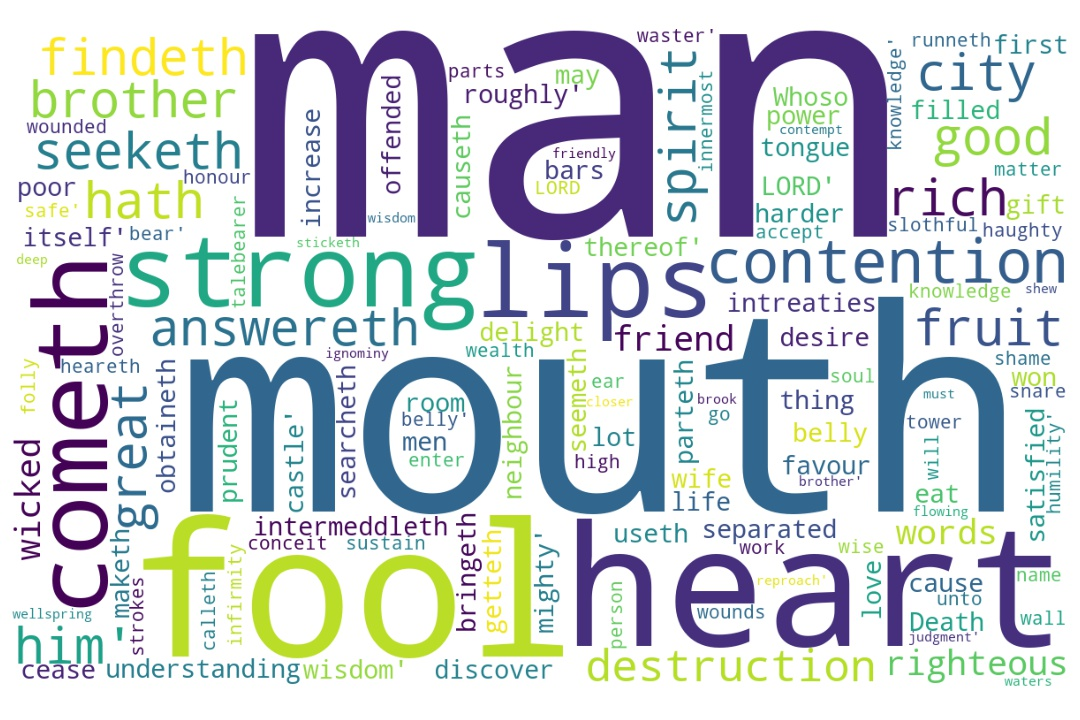
\includegraphics[width=\linewidth]{20OT-Proverbs/Proverb18-WordCloud.jpg}
  \caption{Proverb 18 Word Cloud}
  \label{fig:Proverb 18 word Cloud}
\end{figure}

\marginpar{\scriptsize \centering \fcolorbox{bone}{lime}{\textbf{A MAN FOCUSED ON GOD}}\\ (Proverbs 18:1-24) \begin{compactenum}[I.][8]
    \item Will be an \textbf{Inspired Man} - 
    \item Will be \textbf{Separate from the Ignorant Masses} - 
    \item For him most things in life will have  
    \textbf{Insignificant Meaning} - 
    \item Lives in an \textbf{Isolated Manner} 
    \item Lives by an \textbf{Individual Mandate} 
    \item Has an \textbf{intense and Insular Mentality}
\end{compactenum}}

\marginpar{\scriptsize \centering \fcolorbox{bone}{yellow}{\textbf{A FRIEND LIKE JESUS}}\\ (Proverb 18:24) \begin{compactenum}[I.][8]
    \item A \textbf{Close} Friend
    \item A \textbf{Constant} Friend
    \item A \textbf{Confiding} Friend
    \item A \textbf{Concerned} Friend
    \item A \textbf{Continuing} Friend
    \item A \textbf{Capable} Friend
    \item A \textbf{Caring} Friend
\end{compactenum}}

\marginpar{\scriptsize \centering \fcolorbox{bone}{black}{\textbf{\textcolor{white}{THE PURSUIT OF WISDOM}}}\\ (Proverb 18:24) \begin{compactenum}[I.][8]
    \item Then \textbf{Perverted} Motive -- to learn how manipulate events and circumstances. \index[scripture]{Proverbs!Pro 18:01}(Proverb 18:1)
    \item Then \textbf{Prideful} Motive -- To become exalted as wise. 
    \item Then \textbf{Public} Motive -- to be known and famous. 
    \item Then \textbf{Personal} Motive -- to achieve understanding. 
    \item Then \textbf{Practical} Motive -- to learn how live without mistakes or errors. 
    \item Then \textbf{Purposeful} Motive -- to learn navigate a specific problem. 
    \item Then \textbf{Perfect} Motive -- to learn how to live righteously before God. 
\end{compactenum}}

\marginpar{\scriptsize \centering \fcolorbox{bone}{blue}{\textbf{\textcolor{white}{WHAT YOUR SPEECH REVEALS}}}\\ (Proverb 18:4) \begin{compactenum}[I.][8]
    \item \textbf{Your Education} 
    \item \textbf{Your Excellence} 
    \item \textbf{Your Excitements} 
    \item \textbf{Your Enmity} 
    \item \textbf{Your Enemies} 
    \item \textbf{Your End} 
    \item \textbf{Your Emptiness}
    \item \textbf{Your Entanglements} 
\end{compactenum} }

\marginpar{\scriptsize \centering \fcolorbox{bone}{orange}{\textbf{THE WISE MAN}}\\ (Proverbs 18:1-24) \begin{compactenum}[I.][8]
    \item \textbf{Is Distinctive}
    \item \textbf{Is Disciplined}
    \item \textbf{Ignores Distractions}
    \item \textbf{Finds Delights in Wisdom}
    \item \textbf{Has Departed from the Common and Mundane}
    \item \textbf{Has a Distaste for Foolishness}
    \item \textbf{Is often regarded as Disturbed}
\end{compactenum} }




\footnote{\textcolor[cmyk]{0.99998,1,0,0}{\hyperlink{TOC}{Return to end of Table of Contents.}}}\footnote{\href{https://audiobible.com/bible/proverbs_18.html}{\textcolor[cmyk]{0.99998,1,0,0}{Proverbs Audio}}}\textcolor[cmyk]{0.99998,1,0,0}{Through desire a man, having separated himself, seeketh \emph{and} \fcolorbox{bone}{MYGOLD}{intermeddleth} with all wisdom.}
[2] \textcolor[cmyk]{0.99998,1,0,0}{A fool hath no delight in \fcolorbox{bone}{MYGOLD}{understanding}, but that \fcolorbox{bone}{bone}{his} heart may discover itself.}
[3] \textcolor[cmyk]{0.99998,1,0,0}{When the wicked cometh, \emph{then} cometh also contempt, and with ignominy reproach.}
[4] \textcolor[cmyk]{0.99998,1,0,0}{The words of a man's mouth \emph{are} \emph{as} deep waters, \emph{and} the wellspring of wisdom \emph{as} a flowing brook.}\footnote{\textbf{Proverb 16:22} - Understanding is a wellspring of life unto him that hath it: but the instruction of fools is folly.}
[5] \textcolor[cmyk]{0.99998,1,0,0}{\emph{It} \emph{is} not good to accept the person of the wicked, to overthrow the righteous in judgment.}
[6] \textcolor[cmyk]{0.99998,1,0,0}{A fool's lips enter into contention, and \fcolorbox{bone}{bone}{his} mouth calleth for strokes.}
[7] \textcolor[cmyk]{0.99998,1,0,0}{A fool's mouth \emph{is} \fcolorbox{bone}{bone}{his} destruction, and \fcolorbox{bone}{bone}{his} lips \emph{are} the snare of \fcolorbox{bone}{bone}{his} soul.}
[8] \textcolor[cmyk]{0.99998,1,0,0}{The words of a talebearer \emph{are} as wounds, and they go down into the innermost parts of the belly.}
[9] \textcolor[cmyk]{0.99998,1,0,0}{He also that is slothful in \fcolorbox{bone}{bone}{his} work is brother to him that is a great waster.}
[10] \textcolor[cmyk]{0.99998,1,0,0}{The name of the LORD \emph{is} a strong tower: the righteous runneth into it, and is safe.}
[11] \textcolor[cmyk]{0.99998,1,0,0}{The rich man's wealth \emph{is} \fcolorbox{bone}{bone}{his} strong city, and as an high wall in \fcolorbox{bone}{bone}{his} own conceit.}
[12] \textcolor[cmyk]{0.99998,1,0,0}{Before destruction the heart of man is haughty, and before honour \emph{is} humility.}
[13] \textcolor[cmyk]{0.99998,1,0,0}{He that answereth a matter before he heareth \emph{it}, it \emph{is} folly and shame unto him.}
[14] \textcolor[cmyk]{0.99998,1,0,0}{The spirit of a man will sustain \fcolorbox{bone}{bone}{his} infirmity; but a wounded spirit who can bear?}
[15] \textcolor[cmyk]{0.99998,1,0,0}{The heart of the prudent getteth knowledge; and the ear of the wise seeketh knowledge.}
[16] \textcolor[cmyk]{0.99998,1,0,0}{A man's gift maketh room for him, and bringeth him before great men.}
[17] \textcolor[cmyk]{0.99998,1,0,0}{\emph{He} \emph{that} \emph{is} first in \fcolorbox{bone}{bone}{his} own cause \emph{seemeth} just; but \fcolorbox{bone}{bone}{his} neighbour cometh and searcheth him.}
[18] \textcolor[cmyk]{0.99998,1,0,0}{The lot causeth contentions to cease, and parteth between the mighty.}
[19] \textcolor[cmyk]{0.99998,1,0,0}{A brother offended \emph{is} \emph{harder} \emph{to} \emph{be} \emph{won} than a strong city: and \emph{their} contentions \emph{are} like the bars of a castle.}
[20] \textcolor[cmyk]{0.99998,1,0,0}{A man's belly shall be satisfied with the fruit of \fcolorbox{bone}{bone}{his} mouth; \emph{and} with the increase of \fcolorbox{bone}{bone}{his} lips shall he be filled.}
[21] \textcolor[cmyk]{0.99998,1,0,0}{Death and life \emph{are} in the power of the tongue: and they that love it shall eat the fruit thereof.}
[22] \textcolor[cmyk]{0.99998,1,0,0}{\emph{Whoso} findeth a wife findeth a good \emph{thing}, and obtaineth favour of the LORD.}
[23] \textcolor[cmyk]{0.99998,1,0,0}{The poor useth intreaties; but the rich answereth roughly.}
[24] \textcolor[cmyk]{0.99998,1,0,0}{A man \emph{that} \emph{hath} friends must shew himself friendly: and there is a friend \emph{that} sticketh closer than a brother.}



\index[NWIV]{13!Proverbs!Pro 18:1}\index[AWIP]{Through!Proverbs!Pro 18:1}\index[AWIP]{desire!Proverbs!Pro 18:1}\index[AWIP]{a!Proverbs!Pro 18:1}\index[AWIP]{man!Proverbs!Pro 18:1}\index[AWIP]{having!Proverbs!Pro 18:1}\index[AWIP]{separated!Proverbs!Pro 18:1}\index[AWIP]{himself!Proverbs!Pro 18:1}\index[AWIP]{seeketh!Proverbs!Pro 18:1}\index[AWIP]{\emph{and}!Proverbs!Pro 18:1}\index[AWIP]{intermeddleth!Proverbs!Pro 18:1}\index[AWIP]{with!Proverbs!Pro 18:1}\index[AWIP]{all!Proverbs!Pro 18:1}\index[AWIP]{wisdom!Proverbs!Pro 18:1}\index[AWIP]{\emph{and}!Proverbs!Pro 18:1}

\index[NWIV]{14!Proverbs!Pro 18:2}\index[AWIP]{A!Proverbs!Pro 18:2}\index[AWIP]{fool!Proverbs!Pro 18:2}\index[AWIP]{hath!Proverbs!Pro 18:2}\index[AWIP]{no!Proverbs!Pro 18:2}\index[AWIP]{delight!Proverbs!Pro 18:2}\index[AWIP]{in!Proverbs!Pro 18:2}\index[AWIP]{understanding!Proverbs!Pro 18:2}\index[AWIP]{but!Proverbs!Pro 18:2}\index[AWIP]{that!Proverbs!Pro 18:2}\index[AWIP]{his!Proverbs!Pro 18:2}\index[AWIP]{heart!Proverbs!Pro 18:2}\index[AWIP]{may!Proverbs!Pro 18:2}\index[AWIP]{discover!Proverbs!Pro 18:2}\index[AWIP]{itself!Proverbs!Pro 18:2}

\index[NWIV]{12!Proverbs!Pro 18:3}\index[AWIP]{When!Proverbs!Pro 18:3}\index[AWIP]{the!Proverbs!Pro 18:3}\index[AWIP]{wicked!Proverbs!Pro 18:3}\index[AWIP]{cometh!Proverbs!Pro 18:3}\index[AWIP]{cometh!Proverbs!Pro 18:3 (2)}\index[AWIP]{\emph{then}!Proverbs!Pro 18:3}\index[AWIP]{also!Proverbs!Pro 18:3}\index[AWIP]{contempt!Proverbs!Pro 18:3}\index[AWIP]{and!Proverbs!Pro 18:3}\index[AWIP]{with!Proverbs!Pro 18:3}\index[AWIP]{ignominy!Proverbs!Pro 18:3}\index[AWIP]{reproach!Proverbs!Pro 18:3}\index[AWIP]{\emph{then}!Proverbs!Pro 18:3}

\index[NWIV]{19!Proverbs!Pro 18:4}\index[AWIP]{The!Proverbs!Pro 18:4}\index[AWIP]{words!Proverbs!Pro 18:4}\index[AWIP]{of!Proverbs!Pro 18:4}\index[AWIP]{of!Proverbs!Pro 18:4 (2)}\index[AWIP]{a!Proverbs!Pro 18:4}\index[AWIP]{a!Proverbs!Pro 18:4 (2)}\index[AWIP]{man's!Proverbs!Pro 18:4}\index[AWIP]{mouth!Proverbs!Pro 18:4}\index[AWIP]{\emph{are}!Proverbs!Pro 18:4}\index[AWIP]{\emph{as}!Proverbs!Pro 18:4}\index[AWIP]{\emph{as}!Proverbs!Pro 18:4 (2)}\index[AWIP]{deep!Proverbs!Pro 18:4}\index[AWIP]{waters!Proverbs!Pro 18:4}\index[AWIP]{\emph{and}!Proverbs!Pro 18:4}\index[AWIP]{the!Proverbs!Pro 18:4}\index[AWIP]{wellspring!Proverbs!Pro 18:4}\index[AWIP]{wisdom!Proverbs!Pro 18:4}\index[AWIP]{flowing!Proverbs!Pro 18:4}\index[AWIP]{brook!Proverbs!Pro 18:4}\index[AWIP]{\emph{are}!Proverbs!Pro 18:4}\index[AWIP]{\emph{as}!Proverbs!Pro 18:4}\index[AWIP]{\emph{as}!Proverbs!Pro 18:4 (2)}\index[AWIP]{\emph{and}!Proverbs!Pro 18:4}

\index[NWIV]{17!Proverbs!Pro 18:5}\index[AWIP]{\emph{It}!Proverbs!Pro 18:5}\index[AWIP]{\emph{is}!Proverbs!Pro 18:5}\index[AWIP]{not!Proverbs!Pro 18:5}\index[AWIP]{good!Proverbs!Pro 18:5}\index[AWIP]{to!Proverbs!Pro 18:5}\index[AWIP]{to!Proverbs!Pro 18:5 (2)}\index[AWIP]{accept!Proverbs!Pro 18:5}\index[AWIP]{the!Proverbs!Pro 18:5}\index[AWIP]{the!Proverbs!Pro 18:5 (2)}\index[AWIP]{the!Proverbs!Pro 18:5 (3)}\index[AWIP]{person!Proverbs!Pro 18:5}\index[AWIP]{of!Proverbs!Pro 18:5}\index[AWIP]{wicked!Proverbs!Pro 18:5}\index[AWIP]{overthrow!Proverbs!Pro 18:5}\index[AWIP]{righteous!Proverbs!Pro 18:5}\index[AWIP]{in!Proverbs!Pro 18:5}\index[AWIP]{judgment!Proverbs!Pro 18:5}\index[AWIP]{\emph{It}!Proverbs!Pro 18:5}\index[AWIP]{\emph{is}!Proverbs!Pro 18:5}

\index[NWIV]{12!Proverbs!Pro 18:6}\index[AWIP]{A!Proverbs!Pro 18:6}\index[AWIP]{fool's!Proverbs!Pro 18:6}\index[AWIP]{lips!Proverbs!Pro 18:6}\index[AWIP]{enter!Proverbs!Pro 18:6}\index[AWIP]{into!Proverbs!Pro 18:6}\index[AWIP]{contention!Proverbs!Pro 18:6}\index[AWIP]{and!Proverbs!Pro 18:6}\index[AWIP]{his!Proverbs!Pro 18:6}\index[AWIP]{mouth!Proverbs!Pro 18:6}\index[AWIP]{calleth!Proverbs!Pro 18:6}\index[AWIP]{for!Proverbs!Pro 18:6}\index[AWIP]{strokes!Proverbs!Pro 18:6}

\index[NWIV]{15!Proverbs!Pro 18:7}\index[AWIP]{A!Proverbs!Pro 18:7}\index[AWIP]{fool's!Proverbs!Pro 18:7}\index[AWIP]{mouth!Proverbs!Pro 18:7}\index[AWIP]{\emph{is}!Proverbs!Pro 18:7}\index[AWIP]{his!Proverbs!Pro 18:7}\index[AWIP]{his!Proverbs!Pro 18:7 (2)}\index[AWIP]{his!Proverbs!Pro 18:7 (3)}\index[AWIP]{destruction!Proverbs!Pro 18:7}\index[AWIP]{and!Proverbs!Pro 18:7}\index[AWIP]{lips!Proverbs!Pro 18:7}\index[AWIP]{\emph{are}!Proverbs!Pro 18:7}\index[AWIP]{the!Proverbs!Pro 18:7}\index[AWIP]{snare!Proverbs!Pro 18:7}\index[AWIP]{of!Proverbs!Pro 18:7}\index[AWIP]{soul!Proverbs!Pro 18:7}\index[AWIP]{\emph{is}!Proverbs!Pro 18:7}\index[AWIP]{\emph{are}!Proverbs!Pro 18:7}

\index[NWIV]{19!Proverbs!Pro 18:8}\index[AWIP]{The!Proverbs!Pro 18:8}\index[AWIP]{words!Proverbs!Pro 18:8}\index[AWIP]{of!Proverbs!Pro 18:8}\index[AWIP]{of!Proverbs!Pro 18:8 (2)}\index[AWIP]{a!Proverbs!Pro 18:8}\index[AWIP]{talebearer!Proverbs!Pro 18:8}\index[AWIP]{\emph{are}!Proverbs!Pro 18:8}\index[AWIP]{as!Proverbs!Pro 18:8}\index[AWIP]{wounds!Proverbs!Pro 18:8}\index[AWIP]{and!Proverbs!Pro 18:8}\index[AWIP]{they!Proverbs!Pro 18:8}\index[AWIP]{go!Proverbs!Pro 18:8}\index[AWIP]{down!Proverbs!Pro 18:8}\index[AWIP]{into!Proverbs!Pro 18:8}\index[AWIP]{the!Proverbs!Pro 18:8}\index[AWIP]{the!Proverbs!Pro 18:8 (2)}\index[AWIP]{innermost!Proverbs!Pro 18:8}\index[AWIP]{parts!Proverbs!Pro 18:8}\index[AWIP]{belly!Proverbs!Pro 18:8}\index[AWIP]{\emph{are}!Proverbs!Pro 18:8}

\index[NWIV]{17!Proverbs!Pro 18:9}\index[AWIP]{He!Proverbs!Pro 18:9}\index[AWIP]{also!Proverbs!Pro 18:9}\index[AWIP]{that!Proverbs!Pro 18:9}\index[AWIP]{that!Proverbs!Pro 18:9 (2)}\index[AWIP]{is!Proverbs!Pro 18:9}\index[AWIP]{is!Proverbs!Pro 18:9 (2)}\index[AWIP]{is!Proverbs!Pro 18:9 (3)}\index[AWIP]{slothful!Proverbs!Pro 18:9}\index[AWIP]{in!Proverbs!Pro 18:9}\index[AWIP]{his!Proverbs!Pro 18:9}\index[AWIP]{work!Proverbs!Pro 18:9}\index[AWIP]{brother!Proverbs!Pro 18:9}\index[AWIP]{to!Proverbs!Pro 18:9}\index[AWIP]{him!Proverbs!Pro 18:9}\index[AWIP]{a!Proverbs!Pro 18:9}\index[AWIP]{great!Proverbs!Pro 18:9}\index[AWIP]{waster!Proverbs!Pro 18:9}

\index[NWIV]{17!Proverbs!Pro 18:10}\index[AWIP]{The!Proverbs!Pro 18:10}\index[AWIP]{name!Proverbs!Pro 18:10}\index[AWIP]{of!Proverbs!Pro 18:10}\index[AWIP]{the!Proverbs!Pro 18:10}\index[AWIP]{the!Proverbs!Pro 18:10 (2)}\index[AWIP]{LORD!Proverbs!Pro 18:10}\index[AWIP]{\emph{is}!Proverbs!Pro 18:10}\index[AWIP]{a!Proverbs!Pro 18:10}\index[AWIP]{strong!Proverbs!Pro 18:10}\index[AWIP]{tower!Proverbs!Pro 18:10}\index[AWIP]{righteous!Proverbs!Pro 18:10}\index[AWIP]{runneth!Proverbs!Pro 18:10}\index[AWIP]{into!Proverbs!Pro 18:10}\index[AWIP]{it!Proverbs!Pro 18:10}\index[AWIP]{and!Proverbs!Pro 18:10}\index[AWIP]{is!Proverbs!Pro 18:10}\index[AWIP]{safe!Proverbs!Pro 18:10}\index[AWIP]{\emph{is}!Proverbs!Pro 18:10}

\index[NWIV]{17!Proverbs!Pro 18:11}\index[AWIP]{The!Proverbs!Pro 18:11}\index[AWIP]{rich!Proverbs!Pro 18:11}\index[AWIP]{man's!Proverbs!Pro 18:11}\index[AWIP]{wealth!Proverbs!Pro 18:11}\index[AWIP]{\emph{is}!Proverbs!Pro 18:11}\index[AWIP]{his!Proverbs!Pro 18:11}\index[AWIP]{his!Proverbs!Pro 18:11 (2)}\index[AWIP]{strong!Proverbs!Pro 18:11}\index[AWIP]{city!Proverbs!Pro 18:11}\index[AWIP]{and!Proverbs!Pro 18:11}\index[AWIP]{as!Proverbs!Pro 18:11}\index[AWIP]{an!Proverbs!Pro 18:11}\index[AWIP]{high!Proverbs!Pro 18:11}\index[AWIP]{wall!Proverbs!Pro 18:11}\index[AWIP]{in!Proverbs!Pro 18:11}\index[AWIP]{own!Proverbs!Pro 18:11}\index[AWIP]{conceit!Proverbs!Pro 18:11}\index[AWIP]{\emph{is}!Proverbs!Pro 18:11}

\index[NWIV]{13!Proverbs!Pro 18:12}\index[AWIP]{Before!Proverbs!Pro 18:12}\index[AWIP]{destruction!Proverbs!Pro 18:12}\index[AWIP]{the!Proverbs!Pro 18:12}\index[AWIP]{heart!Proverbs!Pro 18:12}\index[AWIP]{of!Proverbs!Pro 18:12}\index[AWIP]{man!Proverbs!Pro 18:12}\index[AWIP]{is!Proverbs!Pro 18:12}\index[AWIP]{haughty!Proverbs!Pro 18:12}\index[AWIP]{and!Proverbs!Pro 18:12}\index[AWIP]{before!Proverbs!Pro 18:12}\index[AWIP]{honour!Proverbs!Pro 18:12}\index[AWIP]{\emph{is}!Proverbs!Pro 18:12}\index[AWIP]{humility!Proverbs!Pro 18:12}\index[AWIP]{\emph{is}!Proverbs!Pro 18:12}

\index[NWIV]{16!Proverbs!Pro 18:13}\index[AWIP]{He!Proverbs!Pro 18:13}\index[AWIP]{that!Proverbs!Pro 18:13}\index[AWIP]{answereth!Proverbs!Pro 18:13}\index[AWIP]{a!Proverbs!Pro 18:13}\index[AWIP]{matter!Proverbs!Pro 18:13}\index[AWIP]{before!Proverbs!Pro 18:13}\index[AWIP]{he!Proverbs!Pro 18:13}\index[AWIP]{heareth!Proverbs!Pro 18:13}\index[AWIP]{\emph{it}!Proverbs!Pro 18:13}\index[AWIP]{it!Proverbs!Pro 18:13}\index[AWIP]{\emph{is}!Proverbs!Pro 18:13}\index[AWIP]{folly!Proverbs!Pro 18:13}\index[AWIP]{and!Proverbs!Pro 18:13}\index[AWIP]{shame!Proverbs!Pro 18:13}\index[AWIP]{unto!Proverbs!Pro 18:13}\index[AWIP]{him!Proverbs!Pro 18:13}\index[AWIP]{\emph{it}!Proverbs!Pro 18:13}\index[AWIP]{\emph{is}!Proverbs!Pro 18:13}

\index[NWIV]{16!Proverbs!Pro 18:14}\index[AWIP]{The!Proverbs!Pro 18:14}\index[AWIP]{spirit!Proverbs!Pro 18:14}\index[AWIP]{spirit!Proverbs!Pro 18:14 (2)}\index[AWIP]{of!Proverbs!Pro 18:14}\index[AWIP]{a!Proverbs!Pro 18:14}\index[AWIP]{a!Proverbs!Pro 18:14 (2)}\index[AWIP]{man!Proverbs!Pro 18:14}\index[AWIP]{will!Proverbs!Pro 18:14}\index[AWIP]{sustain!Proverbs!Pro 18:14}\index[AWIP]{his!Proverbs!Pro 18:14}\index[AWIP]{infirmity!Proverbs!Pro 18:14}\index[AWIP]{but!Proverbs!Pro 18:14}\index[AWIP]{wounded!Proverbs!Pro 18:14}\index[AWIP]{who!Proverbs!Pro 18:14}\index[AWIP]{can!Proverbs!Pro 18:14}\index[AWIP]{bear?!Proverbs!Pro 18:14}

\index[NWIV]{15!Proverbs!Pro 18:15}\index[AWIP]{The!Proverbs!Pro 18:15}\index[AWIP]{heart!Proverbs!Pro 18:15}\index[AWIP]{of!Proverbs!Pro 18:15}\index[AWIP]{of!Proverbs!Pro 18:15 (2)}\index[AWIP]{the!Proverbs!Pro 18:15}\index[AWIP]{the!Proverbs!Pro 18:15 (2)}\index[AWIP]{the!Proverbs!Pro 18:15 (3)}\index[AWIP]{prudent!Proverbs!Pro 18:15}\index[AWIP]{getteth!Proverbs!Pro 18:15}\index[AWIP]{knowledge!Proverbs!Pro 18:15}\index[AWIP]{knowledge!Proverbs!Pro 18:15 (2)}\index[AWIP]{and!Proverbs!Pro 18:15}\index[AWIP]{ear!Proverbs!Pro 18:15}\index[AWIP]{wise!Proverbs!Pro 18:15}\index[AWIP]{seeketh!Proverbs!Pro 18:15}

\index[NWIV]{13!Proverbs!Pro 18:16}\index[AWIP]{A!Proverbs!Pro 18:16}\index[AWIP]{man's!Proverbs!Pro 18:16}\index[AWIP]{gift!Proverbs!Pro 18:16}\index[AWIP]{maketh!Proverbs!Pro 18:16}\index[AWIP]{room!Proverbs!Pro 18:16}\index[AWIP]{for!Proverbs!Pro 18:16}\index[AWIP]{him!Proverbs!Pro 18:16}\index[AWIP]{him!Proverbs!Pro 18:16 (2)}\index[AWIP]{and!Proverbs!Pro 18:16}\index[AWIP]{bringeth!Proverbs!Pro 18:16}\index[AWIP]{before!Proverbs!Pro 18:16}\index[AWIP]{great!Proverbs!Pro 18:16}\index[AWIP]{men!Proverbs!Pro 18:16}

\index[NWIV]{17!Proverbs!Pro 18:17}\index[AWIP]{\emph{He}!Proverbs!Pro 18:17}\index[AWIP]{\emph{that}!Proverbs!Pro 18:17}\index[AWIP]{\emph{is}!Proverbs!Pro 18:17}\index[AWIP]{first!Proverbs!Pro 18:17}\index[AWIP]{in!Proverbs!Pro 18:17}\index[AWIP]{his!Proverbs!Pro 18:17}\index[AWIP]{his!Proverbs!Pro 18:17 (2)}\index[AWIP]{own!Proverbs!Pro 18:17}\index[AWIP]{cause!Proverbs!Pro 18:17}\index[AWIP]{\emph{seemeth}!Proverbs!Pro 18:17}\index[AWIP]{just!Proverbs!Pro 18:17}\index[AWIP]{but!Proverbs!Pro 18:17}\index[AWIP]{neighbour!Proverbs!Pro 18:17}\index[AWIP]{cometh!Proverbs!Pro 18:17}\index[AWIP]{and!Proverbs!Pro 18:17}\index[AWIP]{searcheth!Proverbs!Pro 18:17}\index[AWIP]{him!Proverbs!Pro 18:17}\index[AWIP]{\emph{He}!Proverbs!Pro 18:17}\index[AWIP]{\emph{that}!Proverbs!Pro 18:17}\index[AWIP]{\emph{is}!Proverbs!Pro 18:17}\index[AWIP]{\emph{seemeth}!Proverbs!Pro 18:17}

\index[NWIV]{11!Proverbs!Pro 18:18}\index[AWIP]{The!Proverbs!Pro 18:18}\index[AWIP]{lot!Proverbs!Pro 18:18}\index[AWIP]{causeth!Proverbs!Pro 18:18}\index[AWIP]{contentions!Proverbs!Pro 18:18}\index[AWIP]{to!Proverbs!Pro 18:18}\index[AWIP]{cease!Proverbs!Pro 18:18}\index[AWIP]{and!Proverbs!Pro 18:18}\index[AWIP]{parteth!Proverbs!Pro 18:18}\index[AWIP]{between!Proverbs!Pro 18:18}\index[AWIP]{the!Proverbs!Pro 18:18}\index[AWIP]{mighty!Proverbs!Pro 18:18}

\index[NWIV]{22!Proverbs!Pro 18:19}\index[AWIP]{A!Proverbs!Pro 18:19}\index[AWIP]{brother!Proverbs!Pro 18:19}\index[AWIP]{offended!Proverbs!Pro 18:19}\index[AWIP]{\emph{is}!Proverbs!Pro 18:19}\index[AWIP]{\emph{harder}!Proverbs!Pro 18:19}\index[AWIP]{\emph{to}!Proverbs!Pro 18:19}\index[AWIP]{\emph{be}!Proverbs!Pro 18:19}\index[AWIP]{\emph{won}!Proverbs!Pro 18:19}\index[AWIP]{than!Proverbs!Pro 18:19}\index[AWIP]{a!Proverbs!Pro 18:19}\index[AWIP]{a!Proverbs!Pro 18:19 (2)}\index[AWIP]{strong!Proverbs!Pro 18:19}\index[AWIP]{city!Proverbs!Pro 18:19}\index[AWIP]{and!Proverbs!Pro 18:19}\index[AWIP]{\emph{their}!Proverbs!Pro 18:19}\index[AWIP]{contentions!Proverbs!Pro 18:19}\index[AWIP]{\emph{are}!Proverbs!Pro 18:19}\index[AWIP]{like!Proverbs!Pro 18:19}\index[AWIP]{the!Proverbs!Pro 18:19}\index[AWIP]{bars!Proverbs!Pro 18:19}\index[AWIP]{of!Proverbs!Pro 18:19}\index[AWIP]{castle!Proverbs!Pro 18:19}\index[AWIP]{\emph{is}!Proverbs!Pro 18:19}\index[AWIP]{\emph{harder}!Proverbs!Pro 18:19}\index[AWIP]{\emph{to}!Proverbs!Pro 18:19}\index[AWIP]{\emph{be}!Proverbs!Pro 18:19}\index[AWIP]{\emph{won}!Proverbs!Pro 18:19}\index[AWIP]{\emph{their}!Proverbs!Pro 18:19}\index[AWIP]{\emph{are}!Proverbs!Pro 18:19}

\index[NWIV]{23!Proverbs!Pro 18:20}\index[AWIP]{A!Proverbs!Pro 18:20}\index[AWIP]{man's!Proverbs!Pro 18:20}\index[AWIP]{belly!Proverbs!Pro 18:20}\index[AWIP]{shall!Proverbs!Pro 18:20}\index[AWIP]{shall!Proverbs!Pro 18:20 (2)}\index[AWIP]{be!Proverbs!Pro 18:20}\index[AWIP]{be!Proverbs!Pro 18:20 (2)}\index[AWIP]{satisfied!Proverbs!Pro 18:20}\index[AWIP]{with!Proverbs!Pro 18:20}\index[AWIP]{with!Proverbs!Pro 18:20 (2)}\index[AWIP]{the!Proverbs!Pro 18:20}\index[AWIP]{the!Proverbs!Pro 18:20 (2)}\index[AWIP]{fruit!Proverbs!Pro 18:20}\index[AWIP]{of!Proverbs!Pro 18:20}\index[AWIP]{of!Proverbs!Pro 18:20 (2)}\index[AWIP]{his!Proverbs!Pro 18:20}\index[AWIP]{his!Proverbs!Pro 18:20 (2)}\index[AWIP]{mouth!Proverbs!Pro 18:20}\index[AWIP]{\emph{and}!Proverbs!Pro 18:20}\index[AWIP]{increase!Proverbs!Pro 18:20}\index[AWIP]{lips!Proverbs!Pro 18:20}\index[AWIP]{he!Proverbs!Pro 18:20}\index[AWIP]{filled!Proverbs!Pro 18:20}\index[AWIP]{\emph{and}!Proverbs!Pro 18:20}

\index[NWIV]{20!Proverbs!Pro 18:21}\index[AWIP]{Death!Proverbs!Pro 18:21}\index[AWIP]{and!Proverbs!Pro 18:21}\index[AWIP]{and!Proverbs!Pro 18:21 (2)}\index[AWIP]{life!Proverbs!Pro 18:21}\index[AWIP]{\emph{are}!Proverbs!Pro 18:21}\index[AWIP]{in!Proverbs!Pro 18:21}\index[AWIP]{the!Proverbs!Pro 18:21}\index[AWIP]{the!Proverbs!Pro 18:21 (2)}\index[AWIP]{the!Proverbs!Pro 18:21 (3)}\index[AWIP]{power!Proverbs!Pro 18:21}\index[AWIP]{of!Proverbs!Pro 18:21}\index[AWIP]{tongue!Proverbs!Pro 18:21}\index[AWIP]{they!Proverbs!Pro 18:21}\index[AWIP]{that!Proverbs!Pro 18:21}\index[AWIP]{love!Proverbs!Pro 18:21}\index[AWIP]{it!Proverbs!Pro 18:21}\index[AWIP]{shall!Proverbs!Pro 18:21}\index[AWIP]{eat!Proverbs!Pro 18:21}\index[AWIP]{fruit!Proverbs!Pro 18:21}\index[AWIP]{thereof!Proverbs!Pro 18:21}\index[AWIP]{\emph{are}!Proverbs!Pro 18:21}

\index[NWIV]{14!Proverbs!Pro 18:22}\index[AWIP]{\emph{Whoso}!Proverbs!Pro 18:22}\index[AWIP]{findeth!Proverbs!Pro 18:22}\index[AWIP]{findeth!Proverbs!Pro 18:22 (2)}\index[AWIP]{a!Proverbs!Pro 18:22}\index[AWIP]{a!Proverbs!Pro 18:22 (2)}\index[AWIP]{wife!Proverbs!Pro 18:22}\index[AWIP]{good!Proverbs!Pro 18:22}\index[AWIP]{\emph{thing}!Proverbs!Pro 18:22}\index[AWIP]{and!Proverbs!Pro 18:22}\index[AWIP]{obtaineth!Proverbs!Pro 18:22}\index[AWIP]{favour!Proverbs!Pro 18:22}\index[AWIP]{of!Proverbs!Pro 18:22}\index[AWIP]{the!Proverbs!Pro 18:22}\index[AWIP]{LORD!Proverbs!Pro 18:22}\index[AWIP]{\emph{Whoso}!Proverbs!Pro 18:22}\index[AWIP]{\emph{thing}!Proverbs!Pro 18:22}

\index[NWIV]{9!Proverbs!Pro 18:23}\index[AWIP]{The!Proverbs!Pro 18:23}\index[AWIP]{poor!Proverbs!Pro 18:23}\index[AWIP]{useth!Proverbs!Pro 18:23}\index[AWIP]{intreaties!Proverbs!Pro 18:23}\index[AWIP]{but!Proverbs!Pro 18:23}\index[AWIP]{the!Proverbs!Pro 18:23}\index[AWIP]{rich!Proverbs!Pro 18:23}\index[AWIP]{answereth!Proverbs!Pro 18:23}\index[AWIP]{roughly!Proverbs!Pro 18:23}

\index[NWIV]{20!Proverbs!Pro 18:24}\index[AWIP]{A!Proverbs!Pro 18:24}\index[AWIP]{man!Proverbs!Pro 18:24}\index[AWIP]{\emph{that}!Proverbs!Pro 18:24}\index[AWIP]{\emph{that}!Proverbs!Pro 18:24 (2)}\index[AWIP]{\emph{hath}!Proverbs!Pro 18:24}\index[AWIP]{friends!Proverbs!Pro 18:24}\index[AWIP]{must!Proverbs!Pro 18:24}\index[AWIP]{shew!Proverbs!Pro 18:24}\index[AWIP]{himself!Proverbs!Pro 18:24}\index[AWIP]{friendly!Proverbs!Pro 18:24}\index[AWIP]{and!Proverbs!Pro 18:24}\index[AWIP]{there!Proverbs!Pro 18:24}\index[AWIP]{is!Proverbs!Pro 18:24}\index[AWIP]{a!Proverbs!Pro 18:24}\index[AWIP]{a!Proverbs!Pro 18:24 (2)}\index[AWIP]{friend!Proverbs!Pro 18:24}\index[AWIP]{sticketh!Proverbs!Pro 18:24}\index[AWIP]{closer!Proverbs!Pro 18:24}\index[AWIP]{than!Proverbs!Pro 18:24}\index[AWIP]{brother!Proverbs!Pro 18:24}\index[AWIP]{\emph{that}!Proverbs!Pro 18:24}\index[AWIP]{\emph{that}!Proverbs!Pro 18:24 (2)}\index[AWIP]{\emph{hath}!Proverbs!Pro 18:24}


\section{Proverb 18 Outlines}

\subsection{My Outlines}

\subsubsection{A Man Focused on God's Wisdom}
\index[speaker]{Keith Anthony!Proverb 18 (A Man Focused on God's Wisdom)}
\index[series]{Proverbs (Keith Anthony)!Pro 18 (A Man Focused on God's Wisdom)}
\index[date]{2014/11/18!Proverb 18 (A Man Focused on God's Wisdom) (Keith Anthony)}
Proverbs 18:1 gives some hints about a man who is ostensibly focused on getting God's wisdom. Can we relate to this kind of person? Do we have any biblical examples? Could it be Elijah, or John the Baptist?
\begin{compactenum}[I.]
    \item Will be an \textbf{Inspired Man} - 
    \item Will be \textbf{Separate from the Ignorant Masses} - 
    \item For him most things in life will have  \textbf{Insignificant Meaning} - 
    \item Lives in an \textbf{Isolated Manner} 
    \item Lives by an \textbf{Individual Mandate} -  seldom supported by friends, and 
    \item Has an \textbf{intense and Insular Mentality} - 
\end{compactenum}
So, this is a guy who is mostly unwanted and unwelcome. Vast majority cannot related to him. How much are you like this man? How much do you want to be? How much do you think you should be?

\subsubsection{A Friend Like Jesus}
\index[speaker]{Keith Anthony!Proverb 18 (A Friend Like Jesus)}
\index[series]{Proverbs (Keith Anthony)!Pro 18 (A Friend Like Jesus)}
\index[date]{2014/11/18!Proverb 18 (A Friend Like Jesus (Keith Anthony)}
\begin{compactenum}[I.][8]
    \item A \textbf{Close} Friend
    \item A \textbf{Constant} Friend
    \item A \textbf{Confiding} Friend
    \item A \textbf{Concerned} Friend
    \item A \textbf{Continuing} Friend
    \item A \textbf{Capable} Friend
    \item A \textbf{Caring} Friend
\end{compactenum}


\subsubsection{The Pursuit of Wisdom}
\index[speaker]{Keith Anthony!Proverb 18 (The Pursuit of Wisdom)}
\index[series]{Proverbs (Keith Anthony)!Pro 18 (The Pursuit of Wisdom)}
\index[date]{2017/03/18!Proverb 18:01 (The Pursuit of Wisdom) (Keith Anthony)}
At issue in the pursuit of wisdom, is the underlying heart motive. I contest that ``Wisdom'' is not a thing, but a person, an individual, who is reading our motives as we go. I also contest that going to wisdom with the wrong motive could lead to disastrous results. Motives range from 100 per cent evil, to (seldom if ever) 100 per cent right. Some of these motives:
\begin{compactenum}[I.]
    \item Then \textbf{Perverted} Motive -- to learn how manipulate events and circumstances. \index[scripture]{Proverbs!Pro 18:01}(Proverb 18:1)
    \item Then \textbf{Prideful} Motive -- To become exalted as wise. 
    \item Then \textbf{Public} Motive -- to be known and famous. 
    \item Then \textbf{Personal} Motive -- to achieve understanding. 
    \item Then \textbf{Practical} Motive -- to learn how live without mistakes or errors. 
    \item Then \textbf{Purposeful} Motive -- to learn navigate a specific problem. 
    \item Then \textbf{Perfect} Motive -- to learn how to live righteously before God. 
\end{compactenum}

\subsubsection{What Your Speech Reveals}
My other main text will be James 3:3-10. which I will quote:  Behold, we put bits in the horses’ mouths, that they may obey us; and we turn about their whole body. [4] Behold also the ships, which though they be so great, and are driven of fierce winds, yet are they turned about with a very small helm, whithersoever the governor listeth. [5] Even so the tongue is a little member, and boasteth great things. Behold, how great a matter a little fire kindleth! [6] And the tongue is a fire, a world of iniquity: so is the tongue among our members, that it defileth the whole body, and setteth on fire the course of nature; and it is set on fire of hell. [7] For every kind of beasts, and of birds, and of serpents, and of things in the sea, is tamed, and hath been tamed of mankind: [8] But the tongue can no man tame; it is an unruly evil, full of deadly poison. [9] Therewith bless we God, even the Father; and therewith curse we men, which are made after the similitude of God. [10] Out of the same mouth proceedeth blessing and cursing. My brethren, these things ought not so to be. [11] Doth a fountain send forth at the same place sweet water and bitter? 12 Can the fig tree, my brethren, bear olive berries? either a vine, figs? so can no fountain both yield salt water and fresh.\\
\\
Consider the verses Proverbs 18:4, Proverbs 18:6, Proverbs 18:7, Proverbs 18:8, and Proverbs 18:13.  These verses say a lot about what people say. What does your speech reveal? Listen to someone long enough and their tongue will betray their innermost secrets ... The things that they love... The things that they focus on... It will reveal if they swim with the deep thinkers or wade in the shallow end of the pool with the other immature and self-focused babies ... Your concept of God, Christianity, and spiritual truth will eventually be reflected in your speech, in casual conversation ... Matthew 26:73, speaking of Peter's denial of Christ, says: And after a while came unto him they that stood by, and said to Peter, Surely thou also art one of them; for thy speech bewrayeth thee.\\
\\
Some things your tongue will tell about you:
\index[speaker]{Keith Anthony!Proverb 18:04 (What Your Speech Reveals)}\\
\index[series]{Proverbs (Keith Anthony)!Pro 18 (What Your Speech Reveals)}
\index[date]{2014/10/18!Proverb 18 (What Your Speech Reveals) (Keith Anthony)}

\index[LOCATION]{Greene County Adult Detention Center!2022/01/18!Tuesday Night}

\begin{compactenum}[I.][10]
    \item \textbf{Your Education} Do you use bad grammar? Intentionally?  Do you use Ebonics?  Is every word, or every other word, out of your mouth a cuss word?  When I say, though, what I really mean is wisdom. 
    \item \textbf{Your Excellence} Or lack of excellence ... If you are a child of God, you are a child of THE King and should talk like it. Back it Daniel 6:3 scripture says, ``Then this Daniel was preferred above the presidents and princes, because an excellent spirit was in him; and the king thought to set him over the whole realm.'' Proverbs 8:6 says: ``Hear; for I will speak of excellent things; and the opening of my lips shall be right things.''
    \item \textbf{Your Excitements} -- what gets you going
    \item \textbf{Your Enmity} -- So, you just can't help with this one ... At some point you're going to speak up on the things that irritate you 
    \item \textbf{Your Enemies} -- who you just might hurt if you had the chance.. But scripture says to let the Lord have vengeance. Nahum 1:2 says: God is jealous, and the LORD revengeth; the LORD revengeth, and is furious; the LORD will take vengeance on his adversaries, and he reserveth wrath for his enemies.
    \item \textbf{Your Enticements} What about that new Corvette?  How about that new Tesla.  I'd sure have fun shooting an AR-15 ... Whata about that new Movie ... and the lead actress?
    \item \textbf{Your Entanglements} -- what preoccupies you is what has you in chains
    \item \textbf{Your Emptiness} A while ago I saw an old friend, who attends a church I used to go to, and who I had not seen in about 5 years. I was expecting a warm ``glad to see you'', but instead got some comment about still being overweight. I guess that gives a measure of that friendship.  Getting more personal, ow many times have we asked ``how are you?'' when we really were not interested in the answer? We spend a great ... Do you or I speak of things that have substance? The problem is that the unsaved really have nothing of substance.
   \item \textbf{Your End} considering the rest of Proverbs, it if usually clear where your road is headed ... Christians often, sometimes usually, talk about heaven.  The lost talk about everything except heaven.  
\end{compactenum}
Matthew 12:36-37 tells us: ``But I say unto you, That every idle word that men shall speak, they shall give account thereof in the day of judgment. [37] For by thy words thou shalt be justified, and by thy words thou shalt be condemned.''\\
\\
So, (1) Consider, (2) Correct, (3) Covert, (4) Control, (5)

\subsubsection{The Wise Man}
\index[speaker]{Keith Anthony!Proverb 18 (The Wise Man)}
\index[series]{Proverbs (Keith Anthony)!Pro 18 (The Wise Man)}
\index[date]{2014/11/18!Proverb 18 (The Wise Man) (Keith Anthony)}
Proverbs 18:1 gives some hints about a wise man:
\begin{compactenum}[I.]
    \item \textbf{Is Distinctive}
    \item \textbf{Is Disciplined}
    \item \textbf{Ignores Distractions}
    \item \textbf{Finds Delights in Wisdom}
    \item \textbf{Has Departed from the Common and Mundane}
    \item \textbf{Has a Distaste for Foolishness}
    \item \textbf{Is often regarded as Disturbed}
\end{compactenum}


\subsection{Outlines from Others}

\subsubsection{What a Friend}
\index[speaker]{Clarence Billheimer!Proverbs 18:24 (What a Friend)}
\index[series]{Proverbs (Clarence Billheimer)!Pro 18:24 (What a Friend)}
\index[date]{2015/04/12!Pro 18:24 (What a Friend) (Clarence Billheimer)}
\textbf{Introduction: } How many of you have friends? How about close friends? How many of you ever lost a friend (other than by death)? How about a close friend? Someone said we can count our true friends on one hand. Having a true friend is really more rare than we think. But the Bible tells us about the Lord Jesus Christ, a true friend, one, who as this passage says, ``sticks closer than a brother.'' Let us look at six things about this true friend, using the letters of the word friend.
\begin{compactenum}[I.]
    \item \textbf{He is faithful} \index[scripture]{1 John!1 John 1:09}(1 John 1:9)
    \item \textbf{He is our redeemer} \index[scripture]{Job!Job 19:25}(Job 19:25)
    \item \textbf{He is interested} \index[scripture]{Philippians!Phil 4:06}(Phil 4:6)
    \item \textbf{He is empathetic} \index[scripture]{Hebrews!Heb 04:15}(Heb 4:15)
    \item \textbf{He is near} \index[scripture]{Hebrews!Heb 13:05}(Heb 13:5)
    \item \textbf{He is our deliverer} (\index[scripture]{2 Samuel!2 Sam 22:02}2 Samuel 22:2, \index[scripture]{Psalm!Psa 18:02}Psalm 18:2)
\end{compactenum}
\textbf{Conclusion: } There are many other things about Jesus Christ that make Him a very special friend. Do you know Him as not only a friend, but as your Savior?

\subsubsection{Jesus, My Best Friend}
\textbf{Creator: }Matthew Hines\\ 
\textbf{Source: }Fundamental Baptist Sermon Outlines\\ 
\index[speaker]{Matthew Hines!Proverbs 18:24 (Jesus, My Best Friend)}
\index[series]{Proverbs (Matthew Hines)!Pro 18:24 (Jesus, My Best Friend)}
\index[date]{2017/17/13!Proverbs 18:24 (Jesus, My Best Friend) (Matthew Hines)}
\textbf{Introduction: } Friends make this life much more enjoyable. There is nothing like serving the Lord with brothers and sisters in Christ. Maybe you fish, hunt, or enjoy other types of activities with those you cherish in this life. We all have special people in our lives that we love to spend time with; however, our best friend should always be the Lord Jesus Christ. In times of trouble, grief, sorrow, and despair, Jesus has been there for you and I. In times of joy, happiness, excitement, and gain, Jesus has been there for you and I!
Notice several things with me about this friendship you and I ought to cherish:
\begin{compactenum}[I.]
    \item The \textbf{PERSON of This Friendship: Gods SON} \index[scripture]{Proverbs!Pro 18:24} (Pro 18:24)
    \item The \textbf{PRICE of This Friendship: SACRIFICE} \index[scripture]{John!John 15:13} (John 15:13)
    \item The \textbf{POWER of This Friendship: Gives me STRENGTH} \index[scripture]{Philippians!Phil 04:13} (Phil 4:13)
    \item The \textbf{PERPETUITY of This Friendship: He is STEDFAST} \index[scripture]{Proverbs!Pro 17:17} (Pro 17:17)
    \item  \textbf{PROOF of This Friendship: SERVICE in His name} \index[scripture]{John!John 14:15} (John 14:15)
    \end{compactenum}
\textbf{Conclusion: } consider these thoughts from the scripture as you go throughout your day. Jesus is the greatest friend you have. He desires that you would know Him on a real and personal level. Do you know him today? If not make a new friend, the best friend you'll ever have!

%\subsubsection{What a Friend}
%\textbf{Creator: }Richard Drummond\\ 
%\textbf{Source: }Fundamental Baptist Sermon Outlines\\ 
%\index[speaker]{Richard Drummond!Proverbs 18:24 (What a Friend)}
%\index[series]{Proverbs (Richard Drummond)!Proverbs 18:24 What a Friend)}
%\index[date]{2017/17/13!Proverbs 18:24 (What a Friend) (Richard Drummond)}
%\textbf{Introduction: } Friends make this life much more enjoyable. There is nothing like serving the Lord with brothers and sisters in Christ. Maybe you fish, hunt, or enjoy other types of activities with those you cherish in this life. We all have special people in our lives that we love to spend time with; however, our best friend should always be the Lord Jesus Christ. In times of trouble, grief, sorrow, and despair, Jesus has been there for you and I. In times of joy, happiness, excitement, and gain, Jesus has been there for you and I!
%Notice several things with me about this friendship you and I ought to cherish:
%\begin{compactenum}[I.]
%%    \item The \textbf{Availability} of a Friend\index[scripture]{Proverbs!Pro 18:24} (Proverb 18:24)
%    \begin{compactenum}[A.]
%    	\item Nature desires friends
%    	\item Need demands friends
%    \end{compactenum}
%    \item The \textbf{Attributes} of a Friend\index[scripture]{Proverbs!Pro 18:24} (Proverb 18:24)
%    \begin{compactenum}[A.]
%    	\item Sympathetic touched when mistreated, sorrow, loss, cries, misunderstood
%    	\item Steadfast - there all the time \index[scripture]{Proverbs!Pro 17:17} (Proverbs 17:17)
%    	\item Strong
%    \end{compactenum}
%    \item The \textbf{Accessibility} of a Friend\index[scripture]{Proverbs!Pro 18:24} (Proverb 18:24)    \begin{compactenum}[A.]
 %   	\item He accepts us \index[scripture]{John!Jhn 6:37} (John. 6:37)
 %   	\item He affirms us \index[scripture]{1 John!1Jn 3:1} (1 John 3:1)
%    	\item He assists \index[scripture]{Philippians!Phil 4:13} (Phil 4:13)
%    \end{compactenum}
%\end{compactenum}







\section{Proverb 18 Comments}

\subsection{Numerical Nuggets}
\textbf{13:} The word ``wellspring'' found only twice in scripture is the 13$^{th}$ word in verse 4. Two thirteen-letter words are in the chapter: ``intermeddleth'' and ``understanding.'' Verse 12, speaking of haughtiness, has 13 words. Verses 1, 12, and 16 have 13 words. Verses 7 and 12 have 13 unique words. The word ``his'' is used 13 times in the chapter. The 13-letter words ``intermeddleth'' and ``understanding'' are used in the chapter.

\subsection{Proverb 18:1-2}
The issue addressed in verses 1 and 2 is the human heart, and as such it should be expected that man will confront and change it, as shown in Table~\ref{table:CorruptionProv18:1}. The verse goes to motive. This is why most (or maybe all) research, ostensibly done for the betterment of mankind, eventually is used to oppress mankind. It comes down to power, position, prestige, prominence, and power. It comes down to why one seeks those things. Verse 2 puts the thought in context: it is the fool who trusts his heart and seeks the heart's desire. Why is this man a fool? It is because a sincere, God-seeking man will quickly elan from scripture the sordid details and depravity of the human heart.\footnote{\textbf{Isaiah 5:21} - Woe unto them that are wise in their own eyes, and prudent in their own sight!}\footnote{\textbf{Luke 10:21} - In that hour Jesus rejoiced in spirit, and said, I thank thee, O Father, Lord of heaven and earth, that thou hast hid these things from the wise and prudent, and hast revealed them unto babes: even so, Father; for so it seemed good in thy sight.}\\
\\
\noindent One commentator explains the process \cite{ruckman1972proverbs}:
\begin{compactenum}[1.]
    \item DESIRE is at the root of all scientific research and investigation (verse 1),
    \item This desire comes form the human HEART and not the human MIND (verse 2),
    \item This desire is essentially subjective, egotistical, and self-seeking (verse 2),
    \item This desire leads a man to pursue the life of isolated superiority, perhaps even the ivory towers of academic, or the esteemed halls of theological institutions, where he deep-down considers himself to be above the masses, or above the common folk. This may even start out as, or continue to masquerade as, a noble cause.
    \item The man does not seek wisdom. He ``seeketh and intermeddleth with all wisdom.'' 
    \item The man's ``love of wisdom'' is neither pure, not objective, not philanthropic.
    \item The wisdom ``sought'' is complete and is a mean's to an end.
\end{compactenum}

\newpage
\begin{center}

\begin{table}[ht]
\centering
\begin{tabular}{|p{.5in}|p{3.5in}|}
    \hline
    \textcolor{blue}{AV} & \textcolor{blue}{Through desire a man, having separated himself, seeketh \emph{and} intermeddleth with all wisdom.}\\ \hline
    \hline
    CEB &  Unfriendly people look out for themselves; they bicker with sensible people.\\ \hline
%
ESV & Whoever isolates himself seeks his own desire;  he breaks out against all sound judgment. \\ \hline
%
NASV &  He who separates himself seeks his own desire, He quarrels against all sound wisdom.\\ \hline
%
MEV & He who separates himself seeks his own desire; he seeks and quarrels against all wisdom.\\ \hline
%
NIV &  An unfriendly person pursues selfish ends and against all sound judgment starts quarrels. \\ \hline
%
NKJV &  A man who isolates himself seeks his own desire; He rages against all wise judgment.\\ \hline
%
RSV &  He who is estranged seeks pretexts  to break out against all sound judgment.\\ \hline \hline

\multicolumn{2}{|p{4.2in}|}{{\textcolor{jungle}{Modern translations, such as the ASV and others, strike out the first part of the verse, concealing the intent of mankind in general.  It goes to the heart's intent in seeking wisdom. How wonderful is the obfuscated RSV text: ``He who is estranged seeks pretexts.'' What does THAT mean?}}} \\ \hline

\end{tabular}
\caption[Corruption Alert: Proverb 18:1]{Corruption Alert: Proverb 18:1} \label{table:Corruption Proverb 18:1}
\end{table}

\end{center}


\newpage


\subsection{Proverb 18 Repeated Phrases}


%%%%%%%%%%
%%%%%%%%%%
\normalsize
 
\begin{center}
\begin{longtable}{|p{3.0in}|p{0.5in}|}
\caption[Proverb 18 Repeated Phrases]{Proverb 18 Repeated Phrases}\label{table:Repeated Phrases Proverb 18} \\
\hline \multicolumn{1}{|c|}{\textbf{Phrase}} & \multicolumn{1}{c|}{\textbf{Frequency}} \\ \hline 
\endfirsthead
 
\multicolumn{2}{c}
{{\bfseries \tablename\ \thetable{} -- continued from previous page}} \\  
\hline \multicolumn{1}{|c|}{\textbf{Phrase}} & \multicolumn{1}{c|}{\textbf{Frequency}} \\ \hline 
\endhead
 
\hline \multicolumn{2}{c}{{ }} \\ \hline
\endfoot 
of the & 7\\ \hline 
of a & 4\\ \hline 
of his & 3\\ \hline 
in his & 3\\ \hline 
\end{longtable}
\end{center}



%%%%%%%%%%
%%%%%%%%%%



%\newpage
\section{Proverb 18 Statistics}

%%%%%%%%%%%%%%%%%%%%%%%%%%%
%%%%% Word Statistics
%%%%%%%%%%%%%%%%%%%%%%%%%%

\normalsize
\subsection{Chapter Word Statistics}


%%%%%%%%%%
%%%%%%%%%%
 
\begin{center}
\begin{longtable}{l|c|c|c|c}
\caption[Stats for Proverb 18]{Stats for Proverb 18} \label{table:Stats for Proverb 18} \\ 
\hline \multicolumn{1}{|c|}{\textbf{Verse(s)}} & \multicolumn{1}{|c|}{\textbf{Count}} & \multicolumn{1}{|c|}{\textbf{Unique}} & \multicolumn{1}{|c|}{\textbf{Italics}} & \multicolumn{1}{|c|}{\textbf{Uniq Italic}}  \\ \hline 
\endfirsthead
 
\multicolumn{5}{c}
{{\bfseries \tablename\ \thetable{} -- continued from previous page}} \\  
\hline \multicolumn{1}{|c|}{\textbf{Verse(s)}} & \multicolumn{1}{|c|}{\textbf{Count}} & \multicolumn{1}{|c|}{\textbf{Unique}} & \multicolumn{1}{|c|}{\textbf{Italics}} & \multicolumn{1}{|c|}{\textbf{Uniq Italic}}  \\ \hline 
\endhead
 
\hline \multicolumn{5}{|r|}{{Continued if needed}} \\ \hline
\endfoot 
1 & 13 & 13 & 1 & 1\\ \hline
2 & 14 & 14 & 0 & 0\\ \hline
3 & 12 & 11 & 1 & 1\\ \hline
4 & 19 & 16 & 4 & 3\\ \hline
5 & 17 & 14 & 2 & 2\\ \hline
6 & 12 & 12 & 0 & 0\\ \hline
7 & 15 & 13 & 2 & 2\\ \hline
8 & 19 & 17 & 1 & 1\\ \hline
9 & 17 & 14 & 0 & 0\\ \hline
10 & 17 & 16 & 1 & 1\\ \hline
11 & 17 & 16 & 1 & 1\\ \hline
12 & 13 & 13 & 1 & 1\\ \hline
13 & 16 & 16 & 2 & 2\\ \hline
14 & 16 & 14 & 0 & 0\\ \hline
15 & 15 & 11 & 0 & 0\\ \hline
16 & 13 & 12 & 0 & 0\\ \hline
17 & 17 & 16 & 4 & 4\\ \hline
18 & 11 & 11 & 0 & 0\\ \hline
19 & 22 & 21 & 7 & 7\\ \hline
20 & 23 & 17 & 1 & 1\\ \hline
21 & 20 & 17 & 1 & 1\\ \hline
22 & 14 & 12 & 2 & 2\\ \hline
23 & 9 & 9 & 0 & 0\\ \hline
24 & 20 & 18 & 3 & 2\\ \hline
\hline \hline
Total & 381 & 190 & 34 & 18




\end{longtable}
\end{center}

%%%%%%%%%%
%%%%%%%%%%


\subsection{Words by Frequency}
%\scriptsize
\begin{center}
\begin{longtable}{l|r}
\caption[Word Frequencies in Proverb 18]{Word Frequencies in Proverb 18} \label{table:WordsIn-Proverb-18} \\ 
\hline \multicolumn{1}{|c|}{\textbf{Word}} & \multicolumn{1}{c|}{\textbf{Frequency}} \\ \hline 
\endfirsthead
  
\multicolumn{2}{c}  
{{\bfseries \tablename\ \thetable{} -- continued from previous page}} \\   
\hline \multicolumn{1}{|c|}{\textbf{Word}} & \multicolumn{1}{c|}{\textbf{Frequency}} \\ \hline   
\endhead  
  
\hline \multicolumn{2}{|r|}{{Continue}} \\ \hline  
\endfoot  
  
\hline \hline  
\endlastfoot  
  
the & 23\\ \hline 
and & 17\\ \hline 
of & 16\\ \hline 
a & 15\\ \hline 
his & 13\\ \hline 
The & 8\\ \hline 
\emph{is} & 8\\ \hline 
A & 7\\ \hline 
in & 6\\ \hline 
is & 6\\ \hline 
that & 5\\ \hline 
\emph{are} & 5\\ \hline 
him & 5\\ \hline 
man & 4\\ \hline 
with & 4\\ \hline 
but & 4\\ \hline 
man's & 4\\ \hline 
mouth & 4\\ \hline 
to & 4\\ \hline 
\emph{and} & 3\\ \hline 
heart & 3\\ \hline 
cometh & 3\\ \hline 
lips & 3\\ \hline 
into & 3\\ \hline 
brother & 3\\ \hline 
strong & 3\\ \hline 
it & 3\\ \hline 
before & 3\\ \hline 
\emph{that} & 3\\ \hline 
shall & 3\\ \hline 
himself & 2\\ \hline 
seeketh & 2\\ \hline 
wisdom & 2\\ \hline 
wicked & 2\\ \hline 
also & 2\\ \hline 
words & 2\\ \hline 
\emph{as} & 2\\ \hline 
good & 2\\ \hline 
righteous & 2\\ \hline 
fool's & 2\\ \hline 
for & 2\\ \hline 
destruction & 2\\ \hline 
as & 2\\ \hline 
they & 2\\ \hline 
belly & 2\\ \hline 
He & 2\\ \hline 
great & 2\\ \hline 
LORD & 2\\ \hline 
rich & 2\\ \hline 
city & 2\\ \hline 
own & 2\\ \hline 
answereth & 2\\ \hline 
he & 2\\ \hline 
spirit & 2\\ \hline 
knowledge & 2\\ \hline 
contentions & 2\\ \hline 
than & 2\\ \hline 
be & 2\\ \hline 
fruit & 2\\ \hline 
findeth & 2\\ \hline 
Through & 1\\ \hline 
desire & 1\\ \hline 
having & 1\\ \hline 
separated & 1\\ \hline 
intermeddleth & 1\\ \hline 
all & 1\\ \hline 
fool & 1\\ \hline 
hath & 1\\ \hline 
no & 1\\ \hline 
delight & 1\\ \hline 
understanding & 1\\ \hline 
may & 1\\ \hline 
discover & 1\\ \hline 
itself & 1\\ \hline 
When & 1\\ \hline 
\emph{then} & 1\\ \hline 
contempt & 1\\ \hline 
ignominy & 1\\ \hline 
reproach & 1\\ \hline 
deep & 1\\ \hline 
waters & 1\\ \hline 
wellspring & 1\\ \hline 
flowing & 1\\ \hline 
brook & 1\\ \hline 
\emph{It} & 1\\ \hline 
not & 1\\ \hline 
accept & 1\\ \hline 
person & 1\\ \hline 
overthrow & 1\\ \hline 
judgment & 1\\ \hline 
enter & 1\\ \hline 
contention & 1\\ \hline 
calleth & 1\\ \hline 
strokes & 1\\ \hline 
snare & 1\\ \hline 
soul & 1\\ \hline 
talebearer & 1\\ \hline 
wounds & 1\\ \hline 
go & 1\\ \hline 
down & 1\\ \hline 
innermost & 1\\ \hline 
parts & 1\\ \hline 
slothful & 1\\ \hline 
work & 1\\ \hline 
waster & 1\\ \hline 
name & 1\\ \hline 
tower & 1\\ \hline 
runneth & 1\\ \hline 
safe & 1\\ \hline 
wealth & 1\\ \hline 
an & 1\\ \hline 
high & 1\\ \hline 
wall & 1\\ \hline 
conceit & 1\\ \hline 
Before & 1\\ \hline 
haughty & 1\\ \hline 
honour & 1\\ \hline 
humility & 1\\ \hline 
matter & 1\\ \hline 
heareth & 1\\ \hline 
\emph{it} & 1\\ \hline 
folly & 1\\ \hline 
shame & 1\\ \hline 
unto & 1\\ \hline 
will & 1\\ \hline 
sustain & 1\\ \hline 
infirmity & 1\\ \hline 
wounded & 1\\ \hline 
who & 1\\ \hline 
can & 1\\ \hline 
bear & 1\\ \hline 
prudent & 1\\ \hline 
getteth & 1\\ \hline 
ear & 1\\ \hline 
wise & 1\\ \hline 
gift & 1\\ \hline 
maketh & 1\\ \hline 
room & 1\\ \hline 
bringeth & 1\\ \hline 
men & 1\\ \hline 
\emph{He} & 1\\ \hline 
first & 1\\ \hline 
cause & 1\\ \hline 
\emph{seemeth} & 1\\ \hline 
just & 1\\ \hline 
neighbour & 1\\ \hline 
searcheth & 1\\ \hline 
lot & 1\\ \hline 
causeth & 1\\ \hline 
cease & 1\\ \hline 
parteth & 1\\ \hline 
between & 1\\ \hline 
mighty & 1\\ \hline 
offended & 1\\ \hline 
\emph{harder} & 1\\ \hline 
\emph{to} & 1\\ \hline 
\emph{be} & 1\\ \hline 
\emph{won} & 1\\ \hline 
\emph{their} & 1\\ \hline 
like & 1\\ \hline 
bars & 1\\ \hline 
castle & 1\\ \hline 
satisfied & 1\\ \hline 
increase & 1\\ \hline 
filled & 1\\ \hline 
Death & 1\\ \hline 
life & 1\\ \hline 
power & 1\\ \hline 
tongue & 1\\ \hline 
love & 1\\ \hline 
eat & 1\\ \hline 
thereof & 1\\ \hline 
\emph{Whoso} & 1\\ \hline 
wife & 1\\ \hline 
\emph{thing} & 1\\ \hline 
obtaineth & 1\\ \hline 
favour & 1\\ \hline 
poor & 1\\ \hline 
useth & 1\\ \hline 
intreaties & 1\\ \hline 
roughly & 1\\ \hline 
\emph{hath} & 1\\ \hline 
friends & 1\\ \hline 
must & 1\\ \hline 
shew & 1\\ \hline 
friendly & 1\\ \hline 
there & 1\\ \hline 
friend & 1\\ \hline 
sticketh & 1\\ \hline 
closer & 1\\ \hline 
\end{longtable}  
\end{center}  


  
\normalsize  

  
  


\subsection{Words Alphabetically}
%\scriptsize
\begin{center}
\begin{longtable}{l|r}
\caption[Word Frequencies in Proverb 18]{Word Frequencies in Proverb 18} \label{table:WordsIn-Proverb-18} \\ 
\hline \multicolumn{1}{|c|}{\textbf{Word}} & \multicolumn{1}{c|}{\textbf{Frequency}} \\ \hline 
\endfirsthead
  
\multicolumn{2}{c}  
{{\bfseries \tablename\ \thetable{} -- continued from previous page}} \\   
\hline \multicolumn{1}{|c|}{\textbf{Word}} & \multicolumn{1}{c|}{\textbf{Frequency}} \\ \hline   
\endhead  
  
\hline \multicolumn{2}{|r|}{{Continue}} \\ \hline  
\endfoot  
  
\hline \hline  
\endlastfoot  
  
A & 7\\ \hline 
Before & 1\\ \hline 
Death & 1\\ \hline 
He & 2\\ \hline 
LORD & 2\\ \hline 
The & 8\\ \hline 
Through & 1\\ \hline 
When & 1\\ \hline 
\emph{He} & 1\\ \hline 
\emph{It} & 1\\ \hline 
\emph{Whoso} & 1\\ \hline 
\emph{and} & 3\\ \hline 
\emph{are} & 5\\ \hline 
\emph{as} & 2\\ \hline 
\emph{be} & 1\\ \hline 
\emph{harder} & 1\\ \hline 
\emph{hath} & 1\\ \hline 
\emph{is} & 8\\ \hline 
\emph{it} & 1\\ \hline 
\emph{seemeth} & 1\\ \hline 
\emph{that} & 3\\ \hline 
\emph{their} & 1\\ \hline 
\emph{then} & 1\\ \hline 
\emph{thing} & 1\\ \hline 
\emph{to} & 1\\ \hline 
\emph{won} & 1\\ \hline 
a & 15\\ \hline 
accept & 1\\ \hline 
all & 1\\ \hline 
also & 2\\ \hline 
an & 1\\ \hline 
and & 17\\ \hline 
answereth & 2\\ \hline 
as & 2\\ \hline 
bars & 1\\ \hline 
be & 2\\ \hline 
bear & 1\\ \hline 
before & 3\\ \hline 
belly & 2\\ \hline 
between & 1\\ \hline 
bringeth & 1\\ \hline 
brook & 1\\ \hline 
brother & 3\\ \hline 
but & 4\\ \hline 
calleth & 1\\ \hline 
can & 1\\ \hline 
castle & 1\\ \hline 
cause & 1\\ \hline 
causeth & 1\\ \hline 
cease & 1\\ \hline 
city & 2\\ \hline 
closer & 1\\ \hline 
cometh & 3\\ \hline 
conceit & 1\\ \hline 
contempt & 1\\ \hline 
contention & 1\\ \hline 
contentions & 2\\ \hline 
deep & 1\\ \hline 
delight & 1\\ \hline 
desire & 1\\ \hline 
destruction & 2\\ \hline 
discover & 1\\ \hline 
down & 1\\ \hline 
ear & 1\\ \hline 
eat & 1\\ \hline 
enter & 1\\ \hline 
favour & 1\\ \hline 
filled & 1\\ \hline 
findeth & 2\\ \hline 
first & 1\\ \hline 
flowing & 1\\ \hline 
folly & 1\\ \hline 
fool & 1\\ \hline 
fool's & 2\\ \hline 
for & 2\\ \hline 
friend & 1\\ \hline 
friendly & 1\\ \hline 
friends & 1\\ \hline 
fruit & 2\\ \hline 
getteth & 1\\ \hline 
gift & 1\\ \hline 
go & 1\\ \hline 
good & 2\\ \hline 
great & 2\\ \hline 
hath & 1\\ \hline 
haughty & 1\\ \hline 
having & 1\\ \hline 
he & 2\\ \hline 
heareth & 1\\ \hline 
heart & 3\\ \hline 
high & 1\\ \hline 
him & 5\\ \hline 
himself & 2\\ \hline 
his & 13\\ \hline 
honour & 1\\ \hline 
humility & 1\\ \hline 
ignominy & 1\\ \hline 
in & 6\\ \hline 
increase & 1\\ \hline 
infirmity & 1\\ \hline 
innermost & 1\\ \hline 
intermeddleth & 1\\ \hline 
into & 3\\ \hline 
intreaties & 1\\ \hline 
is & 6\\ \hline 
it & 3\\ \hline 
itself & 1\\ \hline 
judgment & 1\\ \hline 
just & 1\\ \hline 
knowledge & 2\\ \hline 
life & 1\\ \hline 
like & 1\\ \hline 
lips & 3\\ \hline 
lot & 1\\ \hline 
love & 1\\ \hline 
maketh & 1\\ \hline 
man & 4\\ \hline 
man's & 4\\ \hline 
matter & 1\\ \hline 
may & 1\\ \hline 
men & 1\\ \hline 
mighty & 1\\ \hline 
mouth & 4\\ \hline 
must & 1\\ \hline 
name & 1\\ \hline 
neighbour & 1\\ \hline 
no & 1\\ \hline 
not & 1\\ \hline 
obtaineth & 1\\ \hline 
of & 16\\ \hline 
offended & 1\\ \hline 
overthrow & 1\\ \hline 
own & 2\\ \hline 
parteth & 1\\ \hline 
parts & 1\\ \hline 
person & 1\\ \hline 
poor & 1\\ \hline 
power & 1\\ \hline 
prudent & 1\\ \hline 
reproach & 1\\ \hline 
rich & 2\\ \hline 
righteous & 2\\ \hline 
room & 1\\ \hline 
roughly & 1\\ \hline 
runneth & 1\\ \hline 
safe & 1\\ \hline 
satisfied & 1\\ \hline 
searcheth & 1\\ \hline 
seeketh & 2\\ \hline 
separated & 1\\ \hline 
shall & 3\\ \hline 
shame & 1\\ \hline 
shew & 1\\ \hline 
slothful & 1\\ \hline 
snare & 1\\ \hline 
soul & 1\\ \hline 
spirit & 2\\ \hline 
sticketh & 1\\ \hline 
strokes & 1\\ \hline 
strong & 3\\ \hline 
sustain & 1\\ \hline 
talebearer & 1\\ \hline 
than & 2\\ \hline 
that & 5\\ \hline 
the & 23\\ \hline 
there & 1\\ \hline 
thereof & 1\\ \hline 
they & 2\\ \hline 
to & 4\\ \hline 
tongue & 1\\ \hline 
tower & 1\\ \hline 
understanding & 1\\ \hline 
unto & 1\\ \hline 
useth & 1\\ \hline 
wall & 1\\ \hline 
waster & 1\\ \hline 
waters & 1\\ \hline 
wealth & 1\\ \hline 
wellspring & 1\\ \hline 
who & 1\\ \hline 
wicked & 2\\ \hline 
wife & 1\\ \hline 
will & 1\\ \hline 
wisdom & 2\\ \hline 
wise & 1\\ \hline 
with & 4\\ \hline 
words & 2\\ \hline 
work & 1\\ \hline 
wounded & 1\\ \hline 
wounds & 1\\ \hline 
\end{longtable}  
\end{center}  


  
\normalsize  

  
  
\subsection{Word Lengths in Chapter} 
\normalsize 
\begin{center} 
\begin{longtable}{l|p{3.75in}} 
\caption[Words by Length in Proverb 18]{Words by Length in Proverb 18} \label{table:WordsIn-Proverb-18} \\ 
\hline \multicolumn{1}{|c|}{\textbf{Length}} & \multicolumn{1}{c|}{\textbf{Words}} \\ \hline 
\endfirsthead 
 
\multicolumn{2}{c} 
{{\bfseries \tablename\ \thetable{} -- continued from previous page}} \\ 
\hline \multicolumn{1}{|c|}{\textbf{Length}} & \multicolumn{1}{c|}{\textbf{Words}} \\ \hline 
\endhead 
 
\hline \multicolumn{2}{|r|}{{Continued}} \\ \hline 
\endfoot 
 
\hline \hline 
\endlastfoot 
1 & a, A\\ \hline 
2 & no, in, of, \emph{as}, \emph{It}, \emph{is}, to, as, go, He, is, it, an, he, \emph{it}, \emph{He}, \emph{to}, \emph{be}, be\\ \hline 
3 & man, \emph{and}, all, but, his, may, the, and, The, \emph{are}, not, for, him, own, who, can, ear, men, lot, \emph{won}, eat\\ \hline 
4 & with, fool, hath, that, When, \emph{then}, also, deep, good, lips, into, soul, they, down, work, name, LORD, safe, rich, city, high, wall, unto, will, bear, wise, gift, room, \emph{that}, just, than, like, bars, life, love, wife, poor, \emph{hath}, must, shew\\ \hline 
5 & heart, words, man's, mouth, brook, enter, snare, parts, belly, great, tower, folly, shame, first, cause, cease, \emph{their}, shall, fruit, Death, power, \emph{Whoso}, \emph{thing}, useth, there\\ \hline 
6 & desire, having, wisdom, itself, wicked, cometh, waters, accept, person, fool's, wounds, waster, strong, wealth, Before, before, honour, matter, spirit, maketh, mighty, \emph{harder}, castle, filled, tongue, favour, friend, closer\\ \hline 
7 & Through, himself, seeketh, delight, flowing, calleth, strokes, brother, runneth, conceit, haughty, heareth, sustain, wounded, prudent, getteth, \emph{seemeth}, causeth, parteth, between, thereof, findeth, roughly, friends\\ \hline 
8 & discover, contempt, ignominy, reproach, judgment, slothful, humility, bringeth, offended, increase, friendly, sticketh\\ \hline 
9 & separated, overthrow, righteous, innermost, answereth, infirmity, knowledge, neighbour, searcheth, satisfied, obtaineth\\ \hline 
10 & wellspring, contention, talebearer, intreaties\\ \hline 
11 & destruction, contentions\\ \hline 
13 & intermeddleth, understanding\\ \hline 
\end{longtable} 
\end{center} 




%%%%%%%%%%
%%%%%%%%%%
 

%\input{20OT-Proverbs/Example-DEVOTIONAL-Psalm3-DEVOTIONAL-BryanChapel}


%%% For Indexes

%\index[DEVOTIONAL]{TGIF1!Os Hillman (Living for a Cause Greater Than Yourself) - Proverb 19:17!2021/12/21}

%\index[DEVOTIONAL]{TGIF1!Os Hillman (Living for a Cause Greater Than Yourself) - Proverb 19:17!2021/12/21}

















%%% colour: cardinal red - \textcolor[cmyk]{0,0.85,0.70,0.23}{text}


%%%% Example marginpar with a compactenum list --- green color text
%\marginpar{\scriptsize \textcolor[rgb]{0.00,0.545,0.269}{$\rightarrow$7 Abominations: 
%\begin{compactenum}
%	\item A proud look,
%	\item a lying tongue,
%	\item hands that shed innocent blood,
%	\item An heart that deviseth wicked imaginations,
%	\item feet that be swift in running to mischief,
%	\item A false witness that speaketh lies, and
%	\item he that soweth discord among brethren.
%\end{compactenum}}}



%\newpage

%\begin{mdframed}[style=MyFrame]
%\begin{center}
%\begin{longtable}{|p{.5in}|p{3.5in}|}

%\caption[Corruption Alert: Proverbs 18:1]{Corruption Alert: Proverbs 18:1} \label{table:CorruptionProv18:1} \\ 

%\hline  
%\multicolumn{1}{|c|}{\textbf{Version}} & 
%\multicolumn{1}{c|}{\textbf{Corruption}}  \\ \hline 
%\endfirsthead
 
%\multicolumn{2}{c}
%{{\bfseries \tablename\ \thetable{} -- continued from previous page}} \\  \hline  
%\multicolumn{1}{|c|}{\textbf{Version}} & 
%\multicolumn{1}{c|}{\textbf{Corruption}}  \\ \hline 
%\endhead
 
%\hline \multicolumn{2}{|r|}{{Continued on next page}} \\ \hline
%\endfoot 
%\textcolor[rgb]{0.00,0.00,1.00}{AV} & \textcolor[rgb]{0.00,0.00,1.00}{Through desire a man, having separated himself, seeketh \emph{and} intermeddleth with all wisdom.} \\ \hline
%
%ASV &  He that separateth himself seeketh his own desire, And  rageth against all sound wisdom. \\ \hline
%
%CEB &  Unfriendly people look out for themselves; they bicker with sensible people.\\ \hline
%
%ESV & Whoever isolates himself seeks his own desire;  he breaks out against all sound judgment. \\ \hline
%
%NASV &  He who separates himself seeks his own desire, He quarrels against all sound wisdom.\\ \hline
%
%MEV & He who separates himself seeks his own desire; he seeks and quarrels against all wisdom.\\ \hline
%
%NIV &  An unfriendly person pursues selfish ends and against all sound judgment starts quarrels. \\ \hline
%
%NKJV &  A man who isolates himself seeks his own desire; He rages against all wise judgment.\\ \hline
%
%RSV &  He who is estranged seeks pretexts  to break out against all sound judgment.\\ \hline

% \multicolumn{2}{p{4.3in}}{{Modern translations, such as the ASV and others, strike out the first part of the verse, concealing the intent of mankind in genewisdom clearly revealed in scripture. How wonderful is the obfuscated RSV text: ``He who is estranged seeks pretexts.'' What does THAT mean?}} \\ %\hline

%\hline

%\end{longtable}
%\end{center}

%\normalsize 
%\end{mdframed}

%\marginpar{\scriptsize \centering \fcolorbox{black}{lime}{\textbf{OUTIDE THE PLACE OF PROMISE}}\\ (Psalm 137:1--9) 
%\begin{compactenum}[I.][8]
%	\item \textbf{Plight \& Distress} \index[scripture]{Psalms!Psa 137:01} (Psalm 137:1)
%	\item The \textbf{Place Desired} \index[scripture]{Psalms!Psa 137:01} (Psalm 137:1)
%	\item \textbf{Pining \& Despiar} \index[scripture]{Psalms!Psa 137:02} (Psalm 137:2)
%	\item \textbf{Provoked \& Degraded}\index[scripture]{Psalms!Psa 137:03} (Psalm 137:3)
%	\item The \textbf{Predicament Described}\index[scripture]{Psalms!Psa 137:04} (Psalm 137:4)
%	\item A \textbf{Preference Decided}\index[scripture]{Psalms!Psa 137:06} (Psalm 137:6)
%	\item A \textbf{Prediction of Destruction}\index[scripture]{Psalms!Psa 137:08} (Psalm 137:8)
%\end{compactenum} }


%\subsection{Outlines from Others}

%\subsubsection{Words on Wisdom}
%\index[speaker]{John Battles!Proverbs 01 (Words on Wisdom)}
%\index[series]{Proverbs (John Battles)!Proverbs 01 (Words on Wisdom)}
%\index[date]{2016/01/20!Proverbs 01 (Words on Wisdom) (John Battles)}
%\textbf{Lineage}: adpated from S. Conway\\
%\textbf{Introduction}: Proverbs distinctly points out things that a fool does:
%\begin{compactenum}[I.][4]
%	\item \textbf{Welcome to Wisdom} \index[scripture]{Proverbs!Pro 01:01-09}(Proverbs 1:1-9)
%	\item \textbf{Warnings of Wisdom} \index[scripture]{Proverbs!Pro 01:10-19}(Proverbs 1:10-19).
%	\item \textbf{Woe of Wisdom} \index[scripture]{Proverbs!Pro 01:24-32}(Proverbs 1:24-32)
%	\item \textbf{Watchcare of Wisdom} \index[scripture]{Proverbs!Pro 01:33}(Proverbs 1:33).
%\end{compactenum}


%%%%% COLOR FOR MARGINPAR OUTLINES
%% 1  LIME - \marginpar{\scriptsize \centering \fcolorbox{black}{lime}{\textbf{TITLE}}\\ (Passage) 
%% 2. YELLOW - \marginpar{\scriptsize \centering \fcolorbox{black}{yellow}{\textbf{TITLE}}\\ (Passage) 
%% 3. Blue BGND, WHITE LETTERS - \marginpar{\scriptsize \centering \fcolorbox{black}{blue}{\textbf{\textcolor[cmyk]{0,0,0,0}{TITLE}}}\\ (Passage) 
%% 4. black BGND, WHITE LETTERS - \marginpar{\scriptsize \centering \fcolorbox{black}{black}{\textbf{\textcolor[cmyk]{0,0,0,0}{TITLE}}}\\ (Passage) 
%% 5. red BGND, WHITE LETTERS - \marginpar{\scriptsize \centering \fcolorbox{black}{red}{\textbf{\textcolor[cmyk]{0,0,0,0}{TITLE}}}\\ (Passage) 

%%%%%% INCLUSION OF GRAPHIC
%\newpage

%\begin{figure}
%\begin{center}
%\includegraphics[scale=0.5, angle=90]{07OT-Judges/References/b201107i1-large}
%\caption[Summary of the 13 Judges]{Summary of the 13 Judges}
%\label{fig:Summary of the 13 Judges}
%\end{center}
%\end{figure}


%%%%%%%%%%%
%%%%%%%%%%%

% SYTEMATIC THEOLOGY (10 + 2)
% Theology proper – The study of the character of God
% Angelology – The study of angels
% Biblical theology – The study of the Bible
% Christology – The study of Christ
% Ecclesiology – The study of the church
% Eschatology – The study of the end times[5]
% Hamartiology – The study of sin
% Pneumatology – The study of the Holy Spirit
% Soteriology – The study of salvation
% Theological anthropology – The study of the nature of humanity.
% ++
% Moral theology
% Bilical cosomolgy

%%%%%%%%%%%%%%
%%%%%%%%%%%%%%

% \footnote{\href{https://audiobible.com/bible/psalms_91.html}{\textcolor[cmyk]{0.99998,1,0,0}{Psalm 91 Audio}}}

% \marginpar{\scriptsize \centering \fcolorbox{black}{lime}{\textbf{JERUSALEM}}\\
% \fcolorbox{black}{lime}{\textbf{DON'T GO BACK TO EGYPT}} \\ (Isaiah 31:1--9) 

%%%%%%%%%%%%%%
%%% Extra Colors
%%% from https://latexcolor.blogspot.com/2019/10/list-of-latex-colors.html
%%%%%%%%%%%%%%
% \definecolor{champagne}{rgb}{0.97,0.91,0.81}
% \definecolor{bone}{rgb}{0.89,0.85,0.79}
%\titleJE
%

%%%%% EXAMPLE Index entry:
% \index[DOCTRINES]{Eschatology - Millennium!Psalms!Psa 069:036}

%%% for things found 13 times
%\fcolorbox{black}{bone}{TEXT}
\scriptsize

%%%%%%%%%%%%%%%%%%%%%%%%%%%%%
%Indices

\chapter{Indexes}
\printindex[DOCTRINES]
\printindex[scripture]
\printindex[speaker]
%\printindex[series]

\printindex[FACEBOOK]
\printindex[LOCATION]
\printindex[DEVOTIONAL]
\printindex[AWIP]

\printbibliography
\end{document}

